
%

%\title{\LARGE \textbf{Petit Résumé Pour Alicia}}

%\title{\LARGE \textbf{Petit Résumé Pour ???}}

%\author{
%{\LARGE \textbf{EFFISCICE}}\\[4ex]
%{\large{{\bf Mathématique}  et {\bf Physique}}}\\[9ex]
%{\Large\textbf{VOTRE PRÉINSCRIPTION A DÉJÀ ÉTÉ EFFECTUÉE.}}\\[4ex]
%{\large \textbf{Guillaume THEMEZE}}\\[1ex]
%{\Large\textbf{M2 Physique Fondamentale} , \textbf{M2 Enseignement Supérieur en Physique-Chimie}}\\[1ex]
%{\large {Quantum, Light, Materials and Nano Sciences}}\\[1ex]
%{\large {\url{guillaume.themeze@universite-paris-saclay.fr}}}\\[1ex]
%{\large {}}\\[1ex]
%{\normalsize {}}\\[1ex]
%}
%\date{\today}
%\makeatletter



%\title{\LARGE \textbf{Petit Résumé Pour Alicia}}

%\title{\LARGE \textbf{Léanna est la meilleur !!!}}

%\author{
%{\LARGE \textsf{Léanna est la meilleure !!!}}\\[4ex]
%{\large{{\bf Mathématique}  et {\bf Physique}}}\\[9ex]
%{\Large\textbf{VOTRE PRÉINSCRIPTION A DÉJÀ ÉTÉ EFFECTUÉE.}}\\[4ex]
%{\large \textbf{Guillaume THEMEZE}}\\[1ex]
%{\Large\textbf{M2 Physique Fondamentale}}\\[1ex]
%{\Large\textbf{M2 Enseignement Supérieur en Physique-Chimie}}\\[1ex]
%{\large {Quantum, Light, Materials and Nano Sciences}}\\[1ex]
%{\large {\url{guillaume.themeze@universite-paris-saclay.fr}}}\\[1ex]
%{\large {}}\\[1ex]
%{\normalsize {}}\\[1ex]
%}
%\date{\today}
%\makeatletter


\title{\LARGE \textbf{Quantum inverse scattering method and correlation functions}}

%\title{\LARGE \textbf{Léanna est la meilleur !!!}}

\author{
%{\LARGE \textsf{Léanna est la meilleure !!!}}\\[4ex]
%{\large{{\bf Mathématique}  et {\bf Physique}}}\\[9ex]
%{\Large\textbf{VOTRE PRÉINSCRIPTION A DÉJÀ ÉTÉ EFFECTUÉE.}}\\[4ex]
{\large \textbf{Korepin, N. M. Bogoliubov, A. G. Izergin}}\\[1ex]
%{\Large\textbf{M2 Physique Fondamentale}}\\[1ex]
%{\Large\textbf{M2 Enseignement Supérieur en Physique-Chimie}}\\[1ex]
%{\large {Quantum, Light, Materials and Nano Sciences}}\\[1ex]
%{\large {\url{guillaume.themeze@universite-paris-saclay.fr}}}\\[1ex]
%%{\large {}}\\[1ex]
%{\normalsize {(en cours d'écriture)}}\\[1ex]
%
}
\date{\today}
\makeatletter


%\makeatletter

%\makeindex[intoc=true]
%\makeindex[name=pers,title=Index of person names,intoc=true]

\begin{document}




%\maketitle\\

%%\section{Présentation de l’expérience}
%\section*{Introduction}
%
%\section{Refroidissement}
%
%\section{Imagerie}
%\subsection{Prubleme d'iamgerie et idée numerique}
%
%\section{Confinement transverse}
%
%\section{Confinement longitudinale}
%
%\subsection{Evolution logitudinale}
%
%\section{Outil de sélection spatial}
%
%\subsection{Mesure de distribution de rapidités locales $\rho(x , \theta ) $  pour des systèmes en équilibre}
%
%%\subsection{Piégeage transverses et longitudinale}
%%\section{Outil de sélection spatial}
%%%\section{Mesure de $\rho(x , \theta ) $ }
%
%%\section{Mesure de distribution de rapidités locales $\rho(x , \theta ) $  pour des systèmes en équilibre}

\section*{Introduction}

\begin{itemize}
	\item Objectif du chapitre : présentation synthétique de l’expérience
	\item Distinction claire des contributions : mise en place initiale (précédents doctorants), développement (travail de Léa Dubois), contribution personnelle (prise de données, analyses spécifiques, participation à certaines manipulations)
	\item Rôle de l’expérience dans l’étude de la dynamique des gaz de Bose 1D
\end{itemize}

Ce chapitre présente l’expérience utilisée pour étudier les gaz unidimensionnels de rubidium ultra-froids. Nous décrivons l’architecture du dispositif, les méthodes d’imagerie et d’analyse, ainsi que les protocoles expérimentaux auxquels j’ai participé. Le développement initial du refroidissement et du piégeage avant la puce a été réalisé par d’anciens doctorants. La mise en place du piégeage sur la puce et du système de sélection spatiale à l’aide d’un DMD a été initiée par Léa Dubois, alors en première année de doctorat à mon arrivée. Mon travail s’est concentré principalement sur la prise de données, l’analyse et la participation à certaines expériences spécifiques telles que l’expansion longitudinale et la mesure locale de la distribution de rapidité.


\section{Présentation générale de l’expérience}
\subsection{Vue d’ensemble du dispositif}
\begin{itemize}
    \item Architecture générale : production, piégeage, manipulation et imagerie.
    \item Systèmes étudiés : gaz de rubidium 87 dans des pièges 1D.
    \item Objectifs : exploration de dynamiques hors équilibre.
\end{itemize}

\subsection{Historique et contributions successives}
\begin{itemize}
    \item Étapes de refroidissement et piégeage initial : travaux antérieurs (voir thèses citées).
    \item Développement du piégeage 1D sur puce et du DMD : thèse de Léa Dubois.
    \item Contributions personnelles : prise de données, protocoles dynamiques, analyse.
\end{itemize}

\section{Le dispositif expérimental}
\subsection{Production et refroidissement des atomes (non détaillé ici, renvoi à d'autres travaux)}
\begin{itemize}
    \item Source chaude de rubidium, MOT, molasses optique.
    \item Refroidissement à des températures sub-$\mu~K$ Refroidissement sub-Doppler (détails renvoyés aux travaux précédents).
\end{itemize}

\subsection{Piégeage magnétique sur puce}
\begin{itemize}
    \item Présentation de la puce atomique.
    \item Confinement transverse et longitudinal.
    \item Régime 1D : conditions d’accès (\(\hbar \omega_\perp \gg k_B T\)).
    \item Problèmes de rugosité, stabilité magnétique.
\end{itemize}

\subsection{Génération de potentiels modulés}
\begin{itemize}
    \item Courants modulés pour créer des pièges harmoniques ou quartiques.
    \item Découplage transverse/longitudinal.
\end{itemize}

\section{Sélection spatiale avec DMD}
\subsection{Motivation et principe}
\begin{itemize}
    \item Besoin de préparer des tranches homogènes.
    \item Intérêt dans les protocoles hors équilibre.
\end{itemize}

\subsection{Mise en place technique (initiée par Léa Dubois)}
\begin{itemize}
    \item Dispositif optique de projection.
    \item Contrôle numérique des motifs.
    \item Calibration et stabilité.
\end{itemize}

\subsection{Utilisation dans les protocoles}
\begin{itemize}
    \item Formes utilisées : boîtes, barrières, coupures.
    \item Préparation initiale contrôlée du gaz.
    \item Exemples de protocoles expérimentaux utilisant le DMD
\end{itemize}

\section{Techniques d’imagerie et d’analyse}
\subsection{Imagerie par absorption}
\begin{itemize}
    \item Imagerie \textit{in situ} et après temps de vol.
    \item Résolution, limites instrumentales.
\end{itemize}

\subsection{Analyse des profils}
\begin{itemize}
    \item Extraction des densités, tailles, températures.
    \item Distribution longitudinale.
    \item Estimation de la température par ajustement Yang-Yang (optionnel si pertinent).
\end{itemize}

\section{Expériences et protocoles étudiés}
Cette section peut être la plus personnelle, en précisant ton rôle à chaque fois.
\subsection{Expansion longitudinale}
\begin{itemize}
    \item Protocole d’expansion (libération longitudinale, maintien du confinement transverse).
    \item Suivi de l’évolution du profil.
    \item Analyse à différents temps d’expansion
    \item Comparaison aux modèles analytiques : solutions homothétiques, GP, asymptotiques.
\end{itemize}

\subsection{Sonde locale de distribution de rapidité}
\begin{itemize}
    \item Principe de la mesure : coupure d’une tranche puis expansion.
    \item Rôle du DMD dans la sélection.
    \item Accès à la distribution de vitesse locale.
    \item Comparaison avec les prédictions GHD.
    \item Limites et incertitudes
\end{itemize}

\section{Discussion sur les limites et les perspectives}
\begin{itemize}
    \item Contraintes techniques (bruit, alignement, stabilité de la puce…).
    \item Améliorations potentielles (résolution, contrôle du potentiel, automatisation).
    \item Perspectives pour d’autres types d’expériences (étude de chocs, turbulence quantique, etc.)
\end{itemize}

\section*{Conclusion}
\begin{itemize}
    \item Résumé de l’architecture du dispositif).
    \item Méthodes d’analyse utilisées et robustesse.
    \item Importance de l’expérience dans le contexte de l’étude des gaz quantiques unidimensionnels
\end{itemize}
Ce chapitre a présenté les éléments essentiels du dispositif expérimental, les méthodes d’imagerie, ainsi que les expériences auxquelles j’ai participé. L’ensemble constitue une plateforme performante pour l’étude de la dynamique de gaz 1D hors équilibre.

\appendix
\section*{Annexes}
\begin{itemize}
    \item Schémas techniques (puce, DMD, optique).
    \item Tableaux de paramètres expérimentaux.
    \item Exemples de motifs DMD utilisés.
\end{itemize}

%\begin{abstract}

%\end{abstract}

%\renewcommand{\contentsname}{}%{\vspace{-3cm}} % Ajuste la valeur si besoin

%\begingroup
%\renewcommand{\contentsname}{\vspace{-4cm}}
%\tableofcontents
%\endgroup


%\dominitoc % Active les mini-tables des matières

\tableofcontents

\bigskip

%\listoffigures

%\maketitle\\

%\newpage


                
%\chapter*{Preface}           
%Ce livre est consacré aux solutions exactes des modèles de la théorie quantique des champs (dans une dimension spatiale et une dimension temporelle). Nous étudions également des modèles bidimensionnels de physique statistique classique, qui sont naturellement liés à ces problèmes. Les descriptions complètes des modèles solubles sont données par le Bethe Ansatz, découvert par H. Bethe en 1931 \cite{??}, lors de l'étude de l'antiferromagnétisme de Heisenberg. Le Bethe Ansatz a été très utile pour la résolution de divers problèmes \cite{??, ??, ??, ??}, \cite{??}, \cite{??}, et \cite{??}.

Certains modèles solubles par Bethe Ansatz ont des applications physiques directes. Un problème célèbre résolu par le Bethe Ansatz est le problème de Kondo (voir \cite{??} et \cite{??}). Un autre modèle est le modèle de Hubbard \cite{??}, qui est lié à la supraconductivité à haute température. Une application importante du Bethe Ansatz se trouve en optique non linéaire, où l'émission spontanée coopérative de radiation peut être décrite par un modèle quantique exactement soluble \cite{??}. Le Bethe Ansatz est très utile en physique théorique moderne \cite{??, ??}. Les fonctions de corrélation nous fournissent des informations dynamiques sur le modèle. Elles sont décrites en détail dans ce livre.

Les modèles solubles par Bethe Ansatz ne sont pas libres ; ils généralisent les modèles libres de la théorie quantique des champs dans le sens suivant. La dynamique à plusieurs corps des modèles libres peut être réduite à une dynamique à un corps. Avec le Bethe Ansatz, la dynamique à plusieurs corps peut être réduite à une dynamique à deux corps. La matrice de diffusion pour plusieurs particules est égale au produit de celles à deux particules. Cela conduit à la relation d'auto-consistance pour la matrice de diffusion à deux particules, connue sous le nom de l'équation de Yang-Baxter (un aperçu des articles peut être trouvé dans \cite{??}), qui est le concept central des modèles exactement solubles. Le rôle de l'équation de Yang-Baxter va au-delà de la théorie des systèmes dynamiques. Elle est très importante dans la théorie des nœuds \cite{??} et des groupes quantiques \cite{??}.

Les modèles quantiques exactement solubles sont étroitement liés à la théorie des équations différentielles complètement intégrables. La relation la plus simple est fournie par la limite quasiclassique. Les fonctions de corrélation quantiques sont décrites par des équations différentielles classiques. La méthode moderne pour résoudre ces équations, la méthode de diffusion inverse, a été fondée en 1967 par Gardner, Greene, Kruskal et Miura \cite{??}. Ils ont étudié l'équation de Korteweg-de Vries. P. Lax a montré que cette équation peut être représentée comme une condition de commutativité pour deux opérateurs différentiels linéaires \cite{??}. Il est intéressant de noter que la représentation de Lax est liée algébriquement à l'équation de Yang-Baxter \cite{??}.

La méthode de diffusion inverse a permis de résoudre une large classe d'équations différentielles non linéaires. Le réseau de Toda en est un exemple (voir \cite{??}, \cite{??} et \cite{??}). Ces équations ont des applications dans divers domaines de la physique : la physique des plasmas, l'optique non linéaire, les vagues océaniques non linéaires, et d'autres. Il existe un certain nombre de livres très intéressants sur la méthode de diffusion inverse \cite{??, ??, ??, ??, ??, ??, ??, ??}. On doit également mentionner qu'il existe des équations différentielles complètement intégrables multidimensionnelles. La plus célèbre est l'équation de Yang-Mills autoduale \cite{??}. D'autres exemples sont les équations de Davey-Stewartson \cite{??} et de Kadomtsev-Petviashvili \cite{??}. Les équations différentielles ordinaires complètement intégrables sont également extrêmement importantes ; par exemple, les célèbres équations transcendantes de Painlevé (voir \cite{??} et les références qui y sont citées). Elles apparaissent également en gravitation bidimensionnelle et dans les modèles matriciels (voir \cite{??}, \cite{??}, et \cite{??}) ainsi que dans la description des fonctions de corrélation quantiques \cite{??, ??, ?? et ??}.

Le développement ultérieur de la méthode de diffusion inverse est lié à \cite{??}, où l'interprétation hamiltonienne a été comprise ; L.D. Faddeev et V.E. Zakharov ont montré que la solution d'un modèle par la méthode de diffusion inverse peut être considérée comme une transformation en variables action-angle. Cela offre une opportunité pour la quantification quasiclassique. La théorie quantique des solitons a été construite dans \cite{??, ??, ??, et ??}, où il a été montré qu'après quantification, les solitons apparaissent comme des particules élémentaires dans le spectre du Hamiltonien.

La méthode quantique de diffusion inverse a été découverte dans \cite{??}. Elle offre une vue unifiée de la solution exacte des modèles classiques et quantiques. Elle combine les idées du Bethe Ansatz et de la méthode de diffusion inverse. Le premier modèle à être résolu par la méthode quantique de diffusion inverse était l'équation de Schrödinger non linéaire.


$$i\partial_t \Psi = -\partial_x^2 \Psi + 2c \Psi^\dag \Psi \Psi .$$

La représentation de Lax pour cette équation a été construite dans la référence \cite{??}. Le Bethe Ansatz pour la version quantique de cette équation a été construit dans \cite{??} et \cite{??}. La méthode quantique de diffusion inverse a permis de reproduire les résultats du Bethe Ansatz en partant de la représentation de Lax. Un développement important de la méthode quantique de diffusion inverse est lié à l'étude des équations différentielles pour les fonctions de corrélation quantiques. Il a été montré dans \cite{??} que les équations différentielles pour les fonctions de corrélation quantiques sont simplement reliées à l'équation différentielle originale qui a été quantifiée. Le langage correct pour la description des fonctions de corrélation est celui des fonctions $\tau$. Cela est décrit dans notre livre. Nous devons mentionner les articles \cite{??} et \cite{??} où les équations différentielles ont été obtenues pour la première fois pour les fonctions de corrélation du modèle d'Ising.

La méthode quantique de diffusion inverse est une méthode bien développée (voir les revues \cite{??}, \cite{??}, \cite{??}, \cite{??}, et \cite{??}). Elle a permis de résoudre une large classe d'équations d'évolution non linéaires. Elle explique la nature algébrique du Bethe Ansatz. Notre livre explique cette méthode en détail. Un exemple important résolu par la méthode quantique de diffusion inverse est l'équation de sine-Gordon \cite{??}.


$$\partial_t^2 u - \partial_x^2 u + \frac{m^2}{\beta} \sin \beta u = 0 .$$

En relation avec ce modèle, nous souhaitons mentionner le nouveau livre de Smirnov \cite{Smirnov53}. L'Ansatz de Bethe algébrique est lié aux groupes quantiques \cite{QuantumGroups17}. Il est également profondément lié à la théorie des matrices S factorisées de Zamolodchikov \cite{Zamolodchikov62} et à la théorie des modèles de réseaux exactement solvables en physique statistique classique (la meilleure revue de ces modèles est le livre de Baxter \cite{Baxter5}) ainsi qu'à la théorie conforme des champs \cite{CFT6,CFT30}.

Dans notre livre, nous essayons d'illustrer les énoncés généraux à travers quelques modèles simples. Notre principal exemple est l'équation de Schrödinger non linéaire (dans le cas quantique, il s'agit du modèle d'un gaz de Bose unidimensionnel avec répulsion $\delta$). Nous considérons également le modèle de sine-Gordon, l'antiferromagnétisme de Heisenberg, et le modèle de Hubbard.

Notre livre est divisé en quatre parties, chacune ayant une introduction. La première partie explique l'Ansatz de Bethe en coordonnées. Nous évaluons l'énergie et l'impulsion des excitations ainsi que la matrice de diffusion dans la limite thermodynamique. Normalement, l'état fondamental du modèle est une sphère de Fermi (ou mer de Dirac). La thermodynamique du modèle est construite explicitement.

La deuxième partie explore la méthode de diffusion inverse quantique et l'Ansatz de Bethe algébrique. La classification des modèles exactement solvables y est donnée. Le concept important du déterminant quantique y est introduit (il est lié à l'antipode dans les groupes quantiques). La fonction de partition du modèle à six sommets est représentée comme un déterminant pour le réseau fini avec des conditions aux limites de paroi. Le principe de Pauli pour les bosons en interaction unidimensionnelle est également discuté. Des versions discrètes de modèles continus sont construites de manière à préserver les caractéristiques dynamiques les plus importantes.

Les troisième et quatrième parties décrivent la théorie des fonctions de corrélation. Dans la troisième partie, les fonctions de corrélation quantiques sont représentées comme des déterminants d'opérateurs intégraux (d'une forme très spéciale). La troisième partie commence par une étude algébrique des produits scalaires. Par exemple, il est prouvé que le carré de la norme de la fonction d'onde de Bethe est égal au déterminant de matrices très simples. Cela peut être obtenu par linéarisation des conditions aux limites périodiques (en forme logarithmique) près de la solution. Les fonctions de corrélation sont représentées comme des déterminants d'opérateurs intégraux spéciaux (de type Fredholm).

Dans la quatrième partie, des équations différentielles pour les fonctions de corrélation sont dérivées. Tout d'abord, nous représentons les fonctions de corrélation comme des déterminants de Fredholm d'un certain opérateur intégral. Cet opérateur intégral a une structure très spéciale qui nous permet de le considérer comme un opérateur de Gel'fand-Levitan-Marchenko d'une autre équation différentielle. Cette dernière équation gouverne les fonctions de corrélation. Les asymptotiques des fonctions de corrélation sont évaluées explicitement, même les fonctions de corrélation dépendant du temps et de la température.

Une autre approche des fonctions de corrélation est également discutée. Elle est liée à la théorie conforme des champs quantiques et permet d'évaluer les asymptotiques à longue distance des fonctions de corrélation à température nulle. Les modèles considérés ici sont sans gap, et les fonctions de corrélation décroissent en fonction de la distance ; la température nulle est le point de transition de phase. Ces puissances sont appelées exposants critiques. Elles dépendent de tous les paramètres du modèle et nous les évaluons explicitement. La méthode d'évaluation est liée aux corrections de taille finie. La charge centrale de l'algèbre de Virasoro décrivant les asymptotiques de nos modèles est généralement égale à un.

Les parties du livre sont divisées en chapitres. Les objectifs de chaque chapitre sont expliqués dans une introduction, et à la fin de chaque chapitre, il y a une conclusion qui donne un résumé et contient des commentaires bibliographiques. Les références sont listées par chapitre à la fin du livre.

Il y a une double numérotation des formules dans le livre. Le premier nombre correspond au numéro de la section et le second est le numéro de la formule dans la section. Lorsqu'on fait référence à une formule dans différents chapitres, on précède le numéro de l'équation par le numéro du chapitre. Si nous faisons référence à une section d'un autre chapitre, le numéro de la section sera précédé du numéro du chapitre. Les théorèmes sont numérotés séparément dans chaque chapitre. Les sections marquées d'un astérisque peuvent être omises lors d'une première lecture.

Ce livre a été commencé à Saint-Pétersbourg, où nous avons bénéficié de discussions avec L.D. Faddeev, A.R. Its, N.A. Slavnov, E.K. Sklyanin, N.Yu. Reshetikhin, L.A. Takhtajan, V.E. Zakharov, P.P. Kulish, V.N. Popov, F.A. Smirnov et A.N. Kirillov. Le livre a été terminé à Stony Brook. Nous apprécions grandement l'atmosphère créative de l'Institut de Physique Théorique à Stony Brook. Nous avons bénéficié de discussions avec C.N. Yang, B. McCoy, B. Sutherland, M. Fowler, H. Thacker, H. Flaschka, A. Fokas, A. Newell, M. Ablowitz, J. Palmer, C. Tracy, L.L. Chau, R. Shrock, W. Weisberger, E. Melzer, F. Essler, D. Uglov, H. Frahm, K. Schoutens, F. Figueirido, E. Williams et S. Ray. Les auteurs tiennent à remercier David A. Coker pour la relecture et ses suggestions pédagogiques.

Nous remercions la NSF pour la subvention PHY-9107261.



%parti 1 
%\part{Théorie}

%\chapter{
%%Dans ce chapitre, nous nous intéressons aux fluctuations de la distribution de rapidité \( \delta \rho \) autour d'une distribution de référence \( \rho^c \), qui maximise la contribution à la fonction de partition des états, exprimée comme une fonctionnelle de la distribution \( \rho \) : 

La fonction de partition des états, s'exprime comme une fonctionnelle de la distribution \( \rho \) : 

\begin{eqnarray*}
	\Xi & = & \sum_\rho \exp \left( -\mathcal{A}(\rho) \right).
\end{eqnarray*}  

Dans la section {\em \bf Entropie de Yang-Yang} (\ref{??}), l'action \( \mathcal{A}(\rho) \) s'écrit sous la forme :  

\begin{eqnarray*}
	\mathcal{A}(\rho) & \doteq & - L\mathcal{S}_{YY}(\rho) + L\int f(\theta) \rho (\theta) \, d\theta,		
\end{eqnarray*}  

où \( \mathcal{S}_{YY} \) est la fonctionnelle d'entropie de Yang-Yang, définie dans (\ref{??}), et \( f \) est la fonction paramétrant les charges, introduite dans (\ref{??}).  

Dans cette même section {\em \bf Entropie de Yang-Yang} (\ref{??}), nous avons établi un lien entre \( f \) et distribution de référence \( \rho^c \), qui maximise la contribution à la fonction de partition des états .\\

On veux tester si nos experience est décrit pas un GGE. Pour cela nous nous intéressons aux fluctuations de la distribution de rapidité \( \delta \rho \) autour \( \rho^c \).

%Nous poursuivons à présent avec cette définition de l'action de classe $\mathcal{C}^2$ et admetant une distribution critique $\rho^c$ tel que sa différentielle en ce point critique soit nulle $d\mathcal{A}_{\rho^c} = 0 $ (\ref{??}) de sorte que d'aprés la formule de Taylor-Youg %afin de déterminer les fluctuations autour de \( \Pi^c \). Pour cela, nous réécrivons l'action sous la forme :  

Nous poursuivons à présent avec cette définition de l'action de classe $\mathcal{C}^2$ et admetant une distribution critique $\rho^c$ tel que sa différentielle en ce point critique soit nulle $d\mathcal{A}_{\rho^c} = 0 $ (\ref{??}) de sorte que d'aprés la formule de Taylor-Youg %afin de déterminer les fluctuations autour de \( \Pi^c \). Pour cela, nous réécrivons l'action sous la forme :  

\begin{eqnarray*}  
	\mathcal{A}(\rho^c + \delta \rho) & \underset{ \delta \rho \to 0 }{=} & \mathcal{A}(\rho^c)  + \frac{1}{2} \left. \frac{\delta^2 \mathcal{A}}{\delta \rho^2} \right|_{\rho^c} (\delta \rho) + \mathcal{O}((\delta \rho)^3),  
\end{eqnarray*}  

une expression quadratique pour l'action à l'ordre dominant en \( \delta \Pi \) avec $\left. \frac{\delta^2 \mathcal{A}}{\delta \rho^2} \right|_{\rho^c}$ la forme quadratique définie positive (Fig (\ref{fig.fluctu.A})).

\begin{figure}[H]
	\centering 
	\begin{tikzpicture}
		\begin{scope}[shift={(0,0)}]
			\begin{scope}[transform canvas={scale=0.6}]
				% Définition des couleurs avec les codes HTML
\definecolor{colorOne}{HTML}{443E46}
\definecolor{colorTwo}{HTML}{F6DEB8}
\definecolor{colorThree}{HTML}{908CA4}
\definecolor{colorFour}{HTML}{57659E}
\definecolor{colorFive}{HTML}{C57284}
\definecolor{colorSix}{HTML}{FF5B69}

% Raccourcis pour les couleurs
\def\colorOne{colorOne}
\def\colorTwo{colorTwo}
\def\colorThree{colorThree}
\def\colorFour{colorFour}
\def\colorFive{colorFive}
\def\colorSix{colorSix}

\def\colorslide{blue!50!black}



\begin{scope}
	% Tracer une courbe lisse entre des points
	\draw[shift={(0,0)} ,\colorOne]
		(-1 , 0 ) edge [thick,line width=0.8ex , ->,>=triangle 45  , \colorOne] node [pos = 1 , below ]{\huge$\rho$}( 5  , 0 )
	;
	\draw[shift={(0,0)}, color=\colorOne]
		(0, -1.0 ) edge [thick,line width=0.8ex , ->,>=triangle 45  ]node [pos=0.9,left=0.2cm ]{\huge$\mathcal{A}(\rho)$}( 0  , 5 )
	;
	\draw[]
		(2.5, 0.12 ) edge [thick,line width=0.8ex ,\colorThree ]node [pos=1,below  ]{\huge$\rho^c$} (2.5, -0.12 )	
	;
	
	\draw[]
		(2.5, -0.12 ) edge [thick,line width=0.4ex , dashed, \colorThree ] (2.5, 5.5 )
		(1.5, 1 ) edge [thick,line width=0.4ex , <->,>=triangle 45  , \colorThree ] (3.5, 1 )
		(-0.3,1) edge [thick,line width=0.4ex  , \colorThree ] node [pos=0,left ]{\huge$\mathcal{A}(\rho^c)$} (0.3, 1 )	
	;
    \draw[thick, line width=0.8ex , \colorFour] plot[smooth, tension=0.7] coordinates {
        (1, 5) (1.6 , 3 ) (2.5, 1) (3.5 , 3 )  (4, 5)
    };		
	
\end{scope}

	
			
			\end{scope}
			
			\draw[color = red , scale = 0.5 , draw = none  ] (-2 , -1) rectangle (5, 6) ; 	
		\end{scope}
		
		\begin{scope}[shift={(19,-1)}]
			\begin{scope}[transform canvas={scale=0.6}]
				% Définition des couleurs avec les codes HTML
\definecolor{colorOne}{HTML}{443E46}
\definecolor{colorTwo}{HTML}{F6DEB8}
\definecolor{colorThree}{HTML}{908CA4}
\definecolor{colorFour}{HTML}{57659E}
\definecolor{colorFive}{HTML}{C57284}
\definecolor{colorSix}{HTML}{FF5B69}

% Raccourcis pour les couleurs
\def\colorOne{colorOne}
\def\colorTwo{colorTwo}
\def\colorThree{colorThree}
\def\colorFour{colorFour}
\def\colorFive{colorFive}
\def\colorSix{colorSix}

\def\colorslide{blue!50!black}

\def\Occupation{
	\def\traitx{0.3}
	\def\traity{0.5}
	\draw[shift={(0,0)}]
		(-13.5 , 0 ) edge [thick,line width=0.8ex ]( -3.2  , 0 )
		( -3.2 - \traitx  , 0 - \traity ) edge [thick,line width=0.8ex ]( -3.2 + \traitx  , 0 + \traity  )
		( -2.8 - \traitx  , 0 - \traity ) edge [thick,line width=0.8ex ]( -2.8 + \traitx  , 0 + \traity  )
		(-2.8 , 0 ) edge [thick,line width=0.8ex ](2.8  , 0 )
		( 2.8 - \traitx  , 0 - \traity ) edge [thick,line width=0.8ex ]( 2.8 + \traitx  , 0 + \traity  )
		( 3.2 - \traitx  , 0 - \traity ) edge [thick,line width=0.8ex ]( 3.2 + \traitx  , 0 + \traity  )
		(3.2, 0 ) edge [thick,line width=0.8ex,->,>=triangle 45 , color = black ]node [pos=1.01,below  ]{\huge$\theta$}	( 13  , 0 )
	;
	\draw[shift={(0,0)}, color=\colorOne]
		(-10.5 , -1.5 ) edge [thick,line width=0.8ex , ->,>=triangle 45  ]( -10.5  , 4.5 )
	;
		
	\foreach \r in {1 , ... , 3 } {
%		\draw[
%		decoration={
%		markings,
%    	mark connection node=my node,
%    	mark=at position 0 with{\node [blue,transform shape] (my node) {\large \r};}},
%		color=gray, thick, 
%		line width=0.5ex] decorate { 
%            (-11.0, \r) -- (-10.1, \r )}
%        ;
        \draw[
			color=\colorOne,
			] 
            (-11.0, \r) edge[color=\colorThree , thick,line width=0.5ex] node [pos=-0.5 ]{\large\color{\colorFour} $\frac{\r}{\delta \theta}$ } (-10.3, \r )
        	;
	
	}
	

	
	% Graduation abcsisse 
	% Définitions des listes
% Definitions of the lists
\def\listetuple{-9/\theta_{1}, -8/\theta_{2} , -5/\theta_{3} , -2/\theta_{a-1} , 0/\theta_{a} , 1/\theta_{a+1} , 2/\theta_{a+2} ,  5/\theta_{N-4} , 7/\theta_{N-3},8/\theta_{N-1},9/\theta_{N} }
\def\listetrais{-12 , -11, -10, -9 , -8 , -7 ,  -6 , -5, -4.5,-4, -2 , -1, 0 , 0.5, 1, 2, 4 , 5 ,  6 , 7 , 8 ,8.5, 9 ,  10 , 11, 12 }

% Loop over listetrais
\foreach \r in \listetrais {
    % Initialize found variable to zero
    % Initialize found variable to zero
    %\pgfmathsetmacro\found{0}
    \global\def\found{0}
    \xdef\nomtheta{}
    
    % Check if \r is in listetuple
    \foreach \x/\y in \listetuple { 
        \ifdim \r pt=\x pt % If \r matches any \x in listetuple
            \global\def\found{1} ;
            \xdef\nomtheta{\y} % Set \nomtheta to the corresponding \y
            %\pgfmathsetmacro\found{1} % Set found to 1            
            %\global\pgfmathsetmacro\found{1}
        \fi
    }
    
    %\node [circle, draw, red] (A) at (\r, 2) {\found , $\nomtheta$};
    
    % Draw the line and display \nomtheta if found
    \ifnum\found=1
        \draw[color=\colorOne, thick, line width=0.5ex] 
            (\r, -0.3) -- (\r, 0.3) node[red , pos=-0.5] {\large $\nomtheta$};
         \filldraw[line width=0.5ex, color=\colorSix, outer color=\colorSix, inner color=\colorSix] 
            (\r, 0) circle (4pt);
    \else 
        % Draw without \nomtheta and add a blue circle if not found
        \draw[color=\colorOne, thick, line width=0.5ex] 
            (\r, -0.3) -- (\r, 0.3);
        \filldraw[line width=0.5ex, color=\colorSix, outer color=\colorTwo, inner color=\colorTwo] 
            (\r, 0) circle (4pt); 
    \fi
}

\def\listetrais{-9.5/\theta_{i-1}/2/3, -6.5/\theta_{i}/1/4  ,   -1.5/\theta_{j}/2/4 , 1.5/\theta_{j+1}/-1/3 , 3.5/\theta_{\ell-1}/1/3 , 6.5/\theta_{\ell}/3/4 , 9.5/\theta(\theta_{\ell+1})/-1/3 };



\foreach \r/\nomx/\y/\ys in \listetrais {
	\draw[
		decoration={
		markings,
    	mark connection node=my node,
    	mark=at position .5 with{\node [blue,transform shape] (my node) {\large \color{\colorFour} $\nomx$};}},
		color=\colorThree , thick, 
		line width=0.5ex] decorate { 
            (\r, 0.12) -- (\r, -1.2)}
        ;
     
     \ifdim \y pt > -1 pt 
     	\draw[
			decoration={
			markings,
    		mark connection node=my node,
    		mark=at position .5 with{\node [blue,transform shape] (my node) {\large \color{\colorFour} $\Pi(\nomx) $};}},
			color=\colorThree, thick, 
			line width=0.5ex] decorate { 
            (\r, \y) -- (\r +3, \y)}
        ;
        \draw[
			decoration={
			markings,
    		mark connection node=my node,
    		mark=at position .5 with{\node [blue,transform shape] (my node) {\large \color{\colorFive} $\Pi_s(\nomx) $};}},
			color=\colorFive, thick, 
			line width=0.5ex] decorate { 
            (\r, \ys) -- (\r +3, \ys)}
        ;
     \fi 
     \ifdim \r pt= -1.5 pt
     	\draw[
     		decoration={
			markings,
    		mark connection node=my node,
    		mark=at position .5 with{\node [blue,transform shape] (my node) {\large \color{\colorFour}  $\delta \theta $};},
    		%mark=at position 0.1  with {\arrow[blue, line width=0.5ex]{<}},
    		%mark=at position 1  with {\arrow[blue, line width=0.5ex]{>}}
    		},
        	color=\colorThree,
        	thick,
        	line width=0.5ex,
        	%arrows={Computer Modern Rightarrow[line cap=round]-Computer Modern Rightarrow[line cap=round]}
   			](\r, -1.2) edge[arrows={Computer Modern Rightarrow[line cap=round]-}] (\r + 0.4, -1.2)decorate {
    		(\r, -1.2) -- (\r + 3, -1.2)}(\r + 2, -1.2) edge[arrows={-Computer Modern Rightarrow[line cap=round]}] (\r + 3, -1.2)
    		;
    \fi
			
	
}


			
}


\begin{scope}
	%\draw[help lines , width=1.5ex] (-8,-3) grid (8,3);\draw[help lines ,width=0.5ex , opacity = 0.5] (-3,-3) grid[step=0.1] (3,3));
	
	%\draw[help lines] 
	%	(-3,-3) edge[width=1.5ex] grid (3,3)	
	%	(-3,-3) edge[width=0.5ex , opacity = 0.5] grid (3,3)	
	%;
	\begin{scope}[shift={(0,1)},rotate=0,opacity=1,color=black]
		\Occupation	
		
		%\node[anchor=east, font=\bfseries] at (-11, 0) {\color{red}\large (T = 0 )} ;	
	\end{scope}
	
	
	
	
	\begin{scope}[shift={(-10.5,7)},rotate=0,opacity=1,color=black]
	
	\begin{scope}[shift={(-0,0)},rotate=0,opacity=1,color=black]
	
		\draw[shift={(0,0)} ,line width=1ex,rounded corners = 1ex,color=\colorOne , opacity =1 ,fill=\colorOne!00 , pattern={north east lines} , pattern color=\colorOne!00 ]
			(0 , -1 ) rectangle (5,1)
		;
		

		\begin{scope}[shift={(0.5,0.5)}]
			\draw[color=\colorOne, thick, line width=0.5ex] 
            (0, -0.3) -- (0, 0.3) ;
            \filldraw[line width=0.5ex, color=\colorSix, outer color=\colorSix, inner color=\colorSix] 
            (0, 0) circle (4pt);
            
            \node[anchor=west, font=\bfseries] at (0.2, 0) {\color{\colorSix}\large : quasi-particule};
		\end{scope}
		
		\begin{scope}[shift={(0.5,-0.5)}]
			\draw[color=\colorOne, thick, line width=0.5ex] 
            (0, -0.3) -- (0, 0.3) ;
            \filldraw[line width=0.5ex, color=\colorSix, outer color=\colorTwo, inner color=\colorTwo] 
            (0, 0) circle (4pt);
            
            \node[anchor=west, font=\bfseries] at (0.2, 0) {\color{\colorSix}\large : hole};
		\end{scope}

	\end{scope}
	
	\begin{scope}[shift={(6,0)},rotate=0,opacity=1,color=black]	
		
		\draw[shift={(0,0)} ,line width=1ex,rounded corners = 1ex,color=\colorOne , opacity =1 ,fill=\colorOne!00 , pattern={north east lines} , pattern color=\colorOne!00 ]
			(0 , -1 ) rectangle (7.5,1)
		;
		
		\node[anchor=west] at (0.5, 0.5) {\color{\colorFour}\large $\Pi$ };\node[anchor=west, font=\bfseries] at (1, 0.5) {\color{\colorFour}\large : quasi-particule distribution};
		
		\node[anchor=west] at (0.5, -0.5) {\color{\colorFour}\large $\Pi_h$ };\node[anchor=west, font=\bfseries] at (1, -0.5) {\color{\colorFour}\large  : hole distribution};
		
	\end{scope}
	
	\begin{scope}[shift={(14.5,0)},rotate=0,opacity=1,color=black]	
		
		\draw[shift={(0,0)} ,line width=1ex,rounded corners = 1ex,color=\colorOne , opacity =1 ,fill=\colorOne!00 , pattern={north east lines} , pattern color=\colorOne!00 ]
			(0 , -0.5 ) rectangle (7.0,0.5)
		;
		
		\node[anchor=west] at (0.2, 0) {\color{\colorFour}\large ${\color{\colorFive}\Pi_s} = \Pi + \Pi_h $ } node[anchor=west , font=\bfseries] at (3.1 , 0 )  {\color{\colorFour}\large {\color{\colorFive} : density of states}};
		
	\end{scope}
	
	
	\end{scope}


		
	
\end{scope}

	
			
			\end{scope}
			\begin{scope}[scale=1]
				\draw[color = red , scale = 1 , draw = none  ] (-1 , -1) rectangle (5, 5) ; 
			\end{scope}	
		\end{scope}

		
				
			
	\end{tikzpicture}	
	\captionsetup{skip=10pt} % Ajoute de l’espace après la légende
	\label{fig.fluctu.A}
\end{figure}


On discrétise l'axe des rapidités en  petite cellule de rapidité $[\theta, \theta+\delta\theta]$, qui contient $L\rho(\theta) \delta \theta$ rapidités. 
	



Avec ces petites tranches, la forme quadratique s’écrit :

\begin{eqnarray*}
    \left. \frac{\delta^2 \mathcal{A}}{{\delta \rho}^2} \right|_{\rho^c}(\delta \rho ) &=&  \sum_{a,b \mid \text{tranche}}  
    \delta \rho(\theta_a)  \frac{\partial^2 \mathcal{A}}{\partial \delta \rho(\theta_a) \partial \delta \rho(\theta_b) } (\rho^c)  \delta \rho(\theta_b).
\end{eqnarray*}
Les fluctuations s’écrivent donc :

\begin{eqnarray*}
    \langle \delta \rho ( \theta) \delta \rho ( \theta') \rangle &=&  
    \frac{ \int d\delta \rho \, \delta \rho(\theta) \delta \rho ( \theta') 
    \exp \left( - \frac{1}{2} \sum_{a,b \mid \text{tranche}}  
    \delta \rho(\theta_a) \frac{\partial^2 \mathcal{A}}{\partial \delta \rho(\theta_a) \partial \delta \rho(\theta_b) } (\rho^c)  \delta \rho(\theta_b) \right) }
    { \int d\delta \Pi  
    \exp \left( - \frac{1}{2} \sum_{a,b \mid \text{tranche}}  
    \delta \rho(\theta_a) \frac{\partial^2 \mathcal{A}}{\partial \delta \rho(\theta_a) \partial \delta \rho(\theta_b) } (\rho^c)  \delta \rho(\theta_b) \right) } \\
    &=& \left( \mathbf{A}^{-1} \right)_{\theta , \theta'}
\end{eqnarray*}


\begin{aff}

\begin{eqnarray*}
	\langle \delta \rho ( \theta) \delta \rho ( \theta') \rangle &=& 	\left( \mathbf{A}^{-1} \right)_{\theta , \theta'}
\end{eqnarray*}

	
avec la  {\em matrice hessienne} $\mathbf{A}_{\theta , \theta'} \equiv \frac{\partial^2 \mathcal{A}}{\partial \delta \rho(\theta) \partial \delta \rho(\theta') }(\rho^c)$, au point critique/ qui maximise la probabilité  $\rho^c=\rho^c_s \nu^c $, s'écrit

\begin{eqnarray*}
	\operator{A} & = & \operator{A}^{(0)} + \delta \theta \operator{V}
\end{eqnarray*}

avec 

\begin{eqnarray*}
	A^{(0)}_{\theta , \theta'}  & = &  L\delta \theta \left ( \frac{ 1}{\rho^c_s ( 1  - \nu^c ) \nu^c } \right )(\theta)    \delta({\theta - \theta '})	,\\
	V_{\theta , \theta'}  &= & L \delta \theta \left \{ - \left [ \left ( \frac{1}{\rho^c_s( 1 - \nu^c) } \right ) ( \theta)  +  \left ( \frac{1}{\rho^c_s( 1 - \nu^c) } \right ) ( \theta' )\right ] \frac{ \Delta( \theta'- \theta )}{ 2 \pi } + \int d\theta''  \left ( \frac{\nu^c}{\rho^c_s( 1 - \nu^c) } \right )(\theta'') \frac{\Delta(\theta''- \theta)}{2 \pi}\frac{\Delta(\theta''- \theta')}{2 \pi}   \right \} 	
\end{eqnarray*}

\end{aff}

\subsection{Testes}

\begin{eqnarray*}
	\Delta_{\operator{\mathcal{N}}}^2  & = &  \frac{1}{\beta} \left . \frac{\partial \langle \operator{\mathcal{N}} \rangle}{\partial \mu} \right )_T \\
	\Delta_{\operator{\mathcal{E}}-\mu \operator{\mathcal{N}}}^2  & = &  - \left . \frac{\partial \langle \operator{\mathcal{E}}-\mu \operator{\mathcal{N}} \rangle}{\partial \beta} \right )_\mu 
\end{eqnarray*}

et 

\begin{eqnarray*}
	\Delta_{\operator{\mathcal{N}}}^2  &= & L^2 \int d\theta_a \int d \theta_b \, \langle \delta \rho(\theta_a) \delta \rho(\theta_b) \rangle \\
	\Delta_{\operator{\mathcal{E}}-\mu \operator{\mathcal{N}}}^2  & = & L^2 \int d\theta_a \int d \theta_b \, \left ( - \mu + \frac{1}2 m \theta_a^2  \right  )\left ( - \mu + \frac{1}2 m \theta_b^2  \right  )  \langle \delta \rho(\theta_a) \delta \rho(\theta_b) \rangle
\end{eqnarray*}

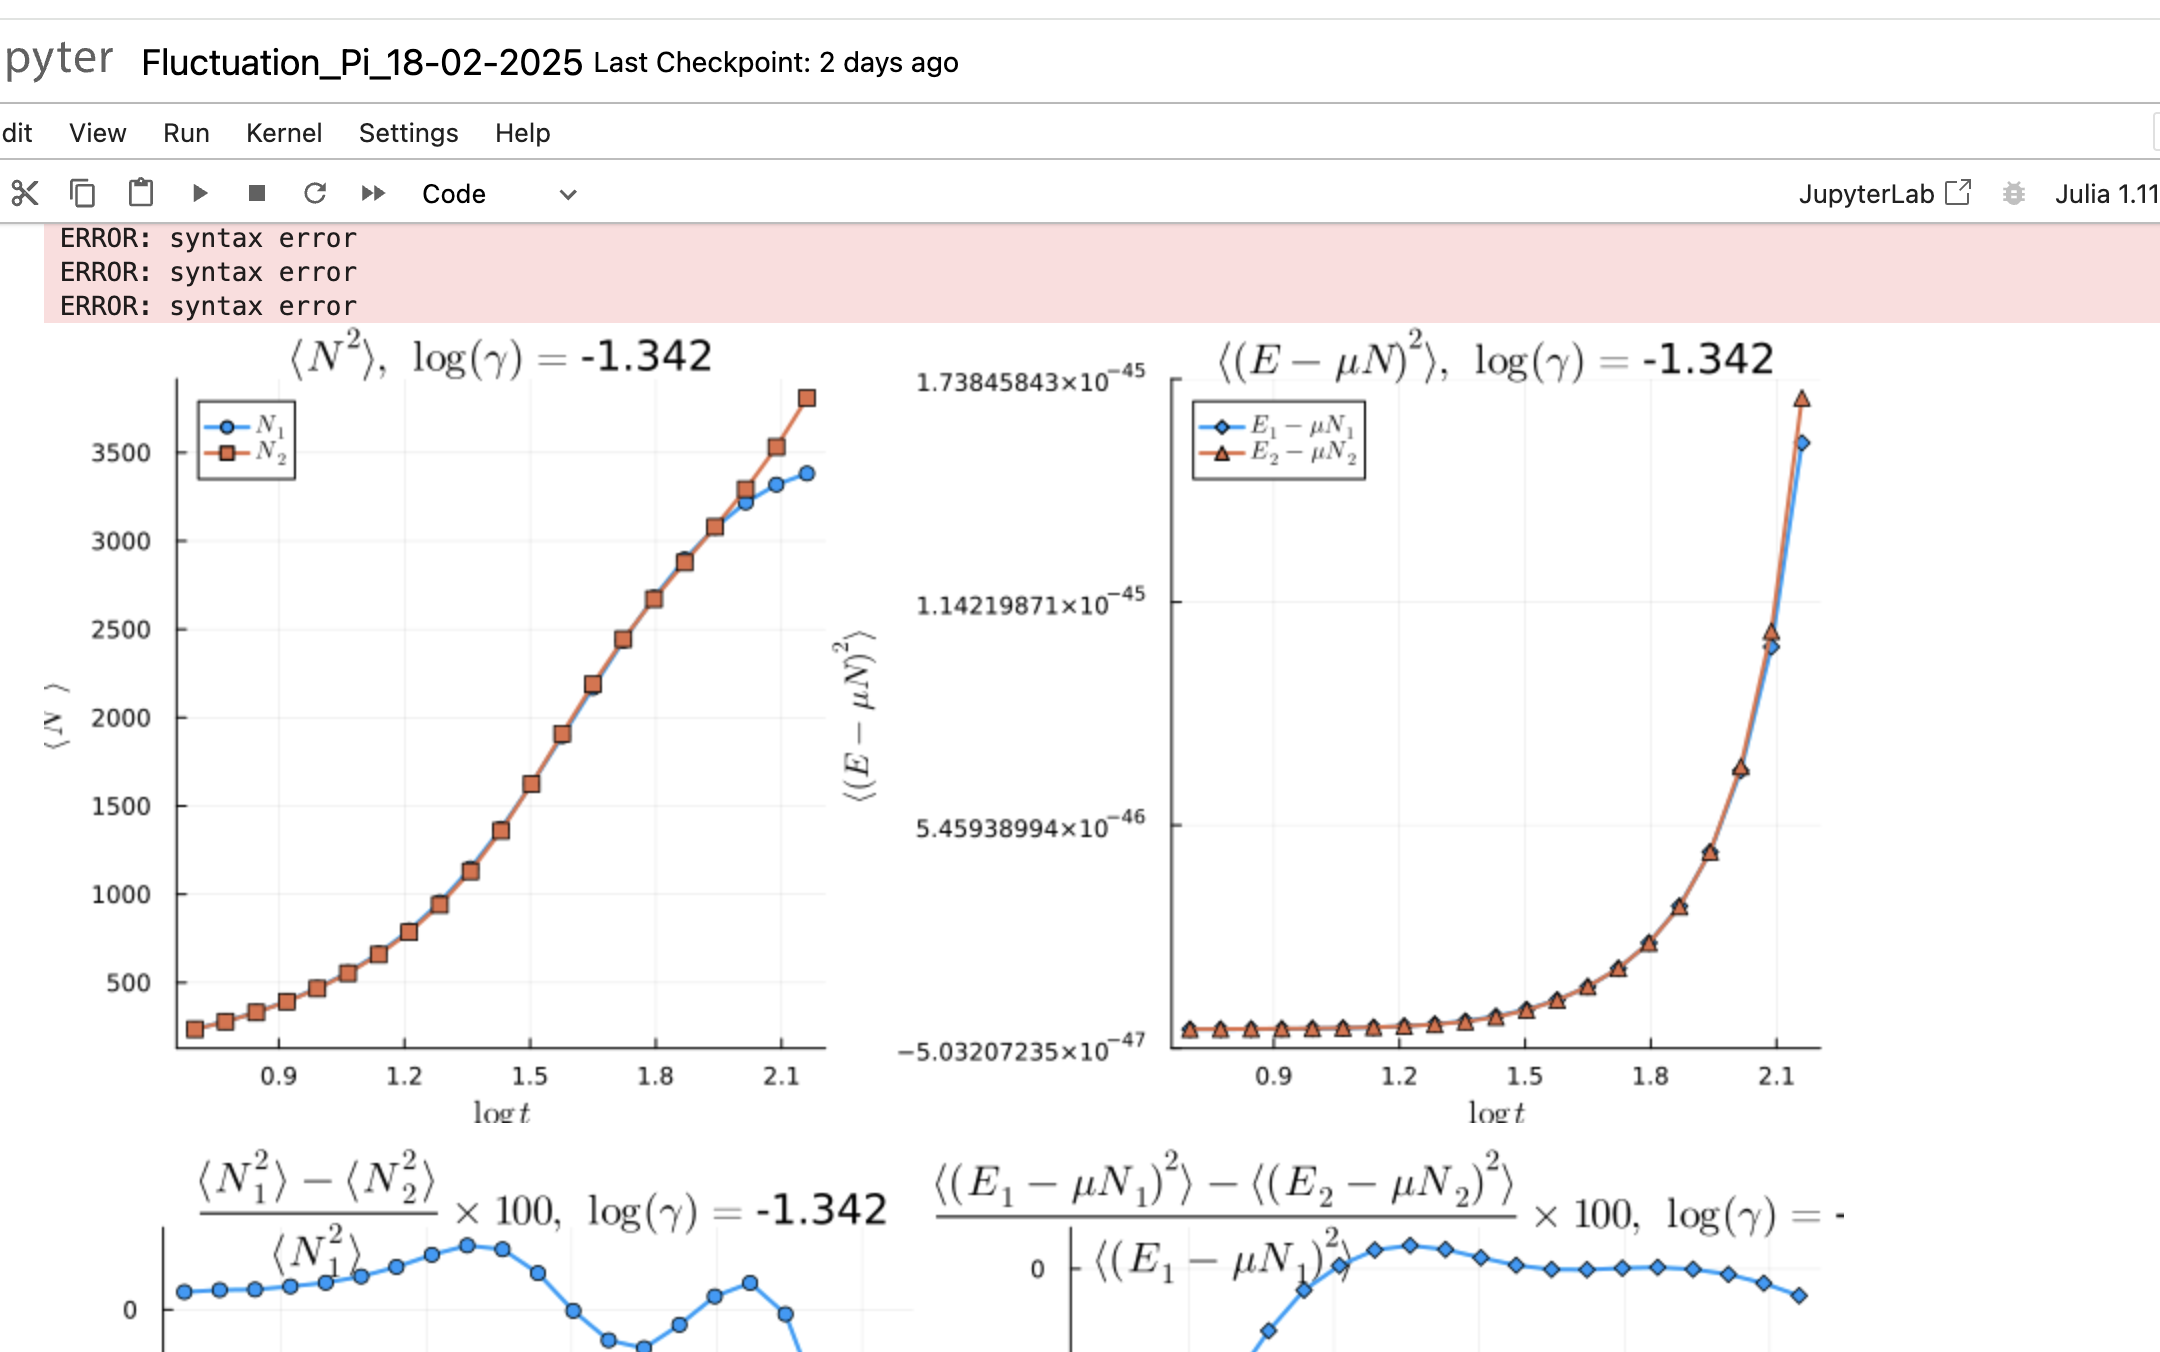
\includegraphics[width=1\textwidth]{Figures/test}

%\begin{aff}
%Donc une a l'ordre un en $\delta \theta (\operator{A}^{(0)})^{-1} %\operator{V}$ 

%\begin{eqnarray*}
%	\langle \delta \Pi ( \theta) \delta \Pi ( \theta') \rangle & = &  ( (\Pi^c_s - \Pi^c)\Pi^c/\Pi^c_s ) ( \theta ) \delta_{\theta, \theta'}/\delta \theta + \mathscr{F}(\theta , \theta' ) ,	
%\end{eqnarray*}

%avec 

%\begin{eqnarray*}
%	\mathscr{F}(\theta , \theta' ) & = & \left [ (\Pi^c_s - \Pi^c )( \theta)  +  (\Pi^c_s - \Pi^c ) ( \theta' )\right ] \frac{\Pi^c}{\Pi^c_s}(\theta)\frac{\Pi^c}{\Pi^c_s}(\theta') \frac{ \Delta( \theta'- \theta )}{ 2 \pi }\\
%	&&  - \left [ (\Pi^c_s - \Pi^c )( \theta)   (\Pi^c_s - \Pi^c ) ( \theta' )\right ] \frac{\Pi^c}{\Pi^c_s}(\theta)\frac{\Pi^c}{\Pi^c_s}(\theta')\int d\theta'' \left (   \frac{ \Pi^c/\Pi^c_s}{\Pi^c_s - \Pi^c} \right )(\theta'') \frac{\Delta(\theta''- \theta)}{2 \pi}\frac{\Delta(\theta''- \theta')}{2 \pi}  	
%\end{eqnarray*}
%\end{aff}



 









%
Chapitre 1 : présente le modèle de Lieb-Liniger, sa solution par Bethe Ansatz, la densité de rapidité à température nulle, et les excitations élémentaires.

Chapitre 2 : développe la thermodynamique du système, introduit le Thermodynamic Bethe Ansatz, les principes statistiques, le GGE, les charges conservées et l’entropie de Yang-Yang.

\chapter{Modèle de Lieb-Liniger et approche Bethe Ansatz}

\section*{Introduction}
Contexte historique et physique du modèle de Lieb-Liniger. Réalisations expérimentales en 1D et rôle de l'intégrabilité. Objectifs du chapitre.

\section{Le modèle de Lieb-Liniger}

\subsection{Hamiltonien du modèle}
\[
\hat{H} = -\sum_{j=1}^N \frac{\partial^2}{\partial x_j^2} + 2c \sum_{1 \leq i < j \leq N} \delta(x_i - x_j)
\]
Présentation des paramètres physiques : interaction $c > 0$, densité $n$, couplage $\gamma$. Conditions aux bords périodiques. Symétrie bosonique.

\subsection{Domaines physiques}
Limite faible interaction (quasi-condensat) et forte interaction (Tonks-Girardeau).

\section{Résolution exacte par Bethe Ansatz}

\subsection{Construction des états propres}
Forme de l’onde : superposition d’ondes planes avec phases. Conditions de raccord au contact.

\subsection{Équations de Bethe}
Conditions aux bords périodiques $\Rightarrow$ quantification des moments $\{k_j\}$.

\subsection{Limite thermodynamique}
Définition des densités $\rho(\lambda)$ et $\rho^h(\lambda)$. Équation intégrale à $T=0$ :
\[
\rho(\lambda) + \rho^h(\lambda) = \frac{1}{2\pi} + \int_{-\infty}^{\infty} K(\lambda - \mu) \rho(\mu) \, d\mu
\]

\section{Propriétés physiques à température nulle}

\subsection{Énergie du fondamental}
Énergie par unité de longueur :
\[
e = \int \lambda^2 \rho(\lambda) \, d\lambda
\]

\subsection{Densité de particules et impulsion}
Formules intégrales. Dépendance en $\gamma$.

\section{Excitations élémentaires à température nulle}

\subsection{Types d’excitations}
Excitations particule-trou. Interprétation via la distribution $\rho$.

\subsection{Relation énergie–impulsion}
Spectre d’excitation (type I et II), vitesse du son $v_s$.

\subsection{Structure de quasi-particules}
Luttinger liquid. Connexions avec la théorie des perturbations.

\section*{Conclusion}
Récapitulatif : solution exacte, densité de rapidité, excitations. Préparation à l’étude thermodynamique.

%%%%%%%%%%%%%%%%%%%%%%%%%%%%%%%%%%%%%%%%%%%%%%%%%%%%%%%%%%%%%%%%%%%%%

\chapter{Thermodynamique du gaz de Lieb-Liniger}

\section*{Introduction}
Problématique : comment définir la thermodynamique d’un système intégrable ? Objectifs du chapitre : TBA, GGE, entropie.

\section{Thermodynamique à température finie : le TBA}

\subsection{Idée générale}
Motivation : accès aux propriétés thermiques. Notion de pseudo-énergie, rôle de l’entropie.

\subsection{Équation de Yang–Yang}
Définition :
\[
\varepsilon(\lambda) = \frac{\lambda^2 - \mu}{T} - \int K(\lambda - \mu') \log\left(1 + e^{-\varepsilon(\mu')} \right) d\mu'
\]

\subsection{Résolution et interprétation}
Accès à $\rho(\lambda)$ à $T>0$. Calculs thermodynamiques.

\section{Statistique quantique et ensemble de Gibbs généralisé (GGE)}

\subsection{Échec de l'ensemble canonique}
Intégrabilité $\Rightarrow$ non thermalisation standard.

\subsection{Définition du GGE}
\[
\rho_{\mathrm{GGE}} = \frac{1}{Z_{\mathrm{GGE}}} \exp\left(-\sum_n \beta_n Q_n\right)
\]

\subsection{Cas du Lieb-Liniger}
Structure des charges $Q_n$, rôle des multiplicateurs $\beta_n$.

\section{Intégrabilité et charges conservées}

\subsection{Définition formelle}
Infinité de charges locales. Lien avec la matrice de transfert.

\subsection{Structure hiérarchique}
Charges de rang élevé, interprétation physique (courants, énergies...).

\subsection{Rôle thermodynamique}
Contraintes fortes sur les états accessibles, impact sur le TBA et le GGE.

\section{Entropie de Yang–Yang}

\subsection{Formule de l’entropie}
\[
s[\rho] = \int d\lambda \left[ (\rho + \rho^h)\log(\rho + \rho^h) - \rho \log \rho - \rho^h \log \rho^h \right]
\]

\subsection{Principe variationnel}
Équilibre thermodynamique = minimisation de
\[
f[\rho] = e[\rho] - T s[\rho]
\]

\subsection{Applications}
Calculs explicites et interprétations physiques.

\section*{Conclusion}
Résumé : TBA, GGE, entropie de Yang–Yang. Perspectives : dynamique hors équilibre, hydrodynamique généralisée.


-----------------------------------

\chapter{Quantification canonique du gaz de Bose unidimensionnel à interaction delta}

\section{Introduction}
Dans ce chapitre, nous présentons la quantification canonique d’un gaz de Bose en une dimension, décrit par un champ de Bose soumis à une interaction de type delta. Ce modèle est fondamental en physique théorique, notamment pour l’étude des systèmes intégrables.

\section{Champs de Bose et relations de commutation}
On introduit le champ de Bose quantique $\Psi(x,t)$ et son adjoint hermitien $\Psi^\dagger(x,t)$, qui satisfont les relations de commutation canoniques à temps égal :
\begin{align}
[\Psi(x), \Psi^\dagger(y)] &= \delta(x - y) \\
[\Psi(x), \Psi(y)] &= [\Psi^\dagger(x), \Psi^\dagger(y)] = 0
\end{align}
Dans ce qui suit, on omettra l’argument temporel $t$ pour alléger les notations.

\section{Hamiltonien du modèle}
Le système est régi par l’Hamiltonien :
\begin{equation}
H = \int dx \left[ (\partial_x \Psi^\dagger)(\partial_x \Psi) + c\, \Psi^\dagger \Psi^\dagger \Psi \Psi \right]
\end{equation}
où $c$ est une constante de couplage.

L’équation du mouvement associée est l’équation de Schrödinger non linéaire :
\begin{equation}
i \partial_t \Psi = -\partial_x^2 \Psi + 2c\, \Psi^\dagger \Psi \Psi
\end{equation}

\section{Le pseudovacuum}
On considère l’état $|0\rangle$ tel que :
\begin{equation}
\Psi(x) |0\rangle = 0, \quad \forall x
\end{equation}
Le dual est défini par $\langle 0| = (|0\rangle)^\dagger$ et vérifie :
\begin{equation}
\langle 0| \Psi^\dagger(x) = 0, \quad \langle 0|0\rangle = 1
\end{equation}
Remarque : $|0\rangle$ n’est pas le vrai vide du système pour $c > 0$ (le vide est un état de type Fermi), mais sert de pseudovacuum pour construire les états excités.

\section{Observables conservées}
Trois opérateurs importants commutent avec le Hamiltonien :
\begin{itemize}
  \item Nombre de particules :
  \[
  Q = \int dx\, \Psi^\dagger(x) \Psi(x)
  \]
  \item Moment total :
  \[
  P = -\frac{i}{2} \int dx\, \left[ \Psi^\dagger \partial_x \Psi - (\partial_x \Psi^\dagger) \Psi \right]
  \]
  \item Hamiltonien $H$
\end{itemize}
Tous ces opérateurs sont hermitiens et satisfont $[H, Q] = [H, P] = 0$.

\section{États propres à N particules}
Un état propre à $N$ particules s’écrit :
\begin{equation}
|\psi(\lambda_1, ..., \lambda_N)\rangle = \frac{1}{\sqrt{N!}} \int d^N z\, \chi_N(z_1,...,z_N|\lambda_1,...,\lambda_N)\, \Psi^\dagger(z_1)\cdots \Psi^\dagger(z_N) |0\rangle
\end{equation}
où $\chi_N$ est une fonction d’onde symétrique des $z_j$, fonction propre du Hamiltonien et du moment total à $N$ corps.

\section{Hamiltonien et moment à N corps}
On définit les opérateurs :
\begin{align}
\mathcal{H}_N &= \sum_{j=1}^N -\partial_{z_j}^2 + 2c \sum_{1 \leq k < j \leq N} \delta(z_j - z_k) \\
\mathcal{P}_N &= \sum_{j=1}^N -i \partial_{z_j}
\end{align}
et les équations aux valeurs propres :
\begin{align}
\mathcal{H}_N \chi_N &= E_N \chi_N \\
\mathcal{P}_N \chi_N &= p_N \chi_N
\end{align}

\section{Action de l’opérateur moment}
L’action de l’opérateur $P$ sur $|\psi_N\rangle$ est :
\[
P |\psi_N\rangle = i \int dx\, (\partial_x \Psi^\dagger) \Psi\, |\psi_N\rangle
\]
On utilise les relations de commutation et des intégrations par parties pour obtenir :
\[
P |\psi_N\rangle = \frac{1}{\sqrt{N!}} \int d^N z\, \left( \sum_{k=1}^N -i \partial_{z_k} \right) \chi_N(z_1,...,z_N)\, \Psi^\dagger(z_1)\cdots \Psi^\dagger(z_N)|0\rangle
\]
ce qui confirme que l’état est bien un vecteur propre de l’opérateur moment avec valeur propre $p_N = \sum_k \lambda_k$ si $\chi_N$ est une onde plane symétrisée.






\chapter{Modèle de Lieb-Liniger et approche Bethe Ansatz}
\minitoc
%Dans ce chapitre, nous nous intéressons aux fluctuations de la distribution de rapidité \( \delta \rho \) autour d'une distribution de référence \( \rho^c \), qui maximise la contribution à la fonction de partition des états, exprimée comme une fonctionnelle de la distribution \( \rho \) : 

La fonction de partition des états, s'exprime comme une fonctionnelle de la distribution \( \rho \) : 

\begin{eqnarray*}
	\Xi & = & \sum_\rho \exp \left( -\mathcal{A}(\rho) \right).
\end{eqnarray*}  

Dans la section {\em \bf Entropie de Yang-Yang} (\ref{??}), l'action \( \mathcal{A}(\rho) \) s'écrit sous la forme :  

\begin{eqnarray*}
	\mathcal{A}(\rho) & \doteq & - L\mathcal{S}_{YY}(\rho) + L\int f(\theta) \rho (\theta) \, d\theta,		
\end{eqnarray*}  

où \( \mathcal{S}_{YY} \) est la fonctionnelle d'entropie de Yang-Yang, définie dans (\ref{??}), et \( f \) est la fonction paramétrant les charges, introduite dans (\ref{??}).  

Dans cette même section {\em \bf Entropie de Yang-Yang} (\ref{??}), nous avons établi un lien entre \( f \) et distribution de référence \( \rho^c \), qui maximise la contribution à la fonction de partition des états .\\

On veux tester si nos experience est décrit pas un GGE. Pour cela nous nous intéressons aux fluctuations de la distribution de rapidité \( \delta \rho \) autour \( \rho^c \).

%Nous poursuivons à présent avec cette définition de l'action de classe $\mathcal{C}^2$ et admetant une distribution critique $\rho^c$ tel que sa différentielle en ce point critique soit nulle $d\mathcal{A}_{\rho^c} = 0 $ (\ref{??}) de sorte que d'aprés la formule de Taylor-Youg %afin de déterminer les fluctuations autour de \( \Pi^c \). Pour cela, nous réécrivons l'action sous la forme :  

Nous poursuivons à présent avec cette définition de l'action de classe $\mathcal{C}^2$ et admetant une distribution critique $\rho^c$ tel que sa différentielle en ce point critique soit nulle $d\mathcal{A}_{\rho^c} = 0 $ (\ref{??}) de sorte que d'aprés la formule de Taylor-Youg %afin de déterminer les fluctuations autour de \( \Pi^c \). Pour cela, nous réécrivons l'action sous la forme :  

\begin{eqnarray*}  
	\mathcal{A}(\rho^c + \delta \rho) & \underset{ \delta \rho \to 0 }{=} & \mathcal{A}(\rho^c)  + \frac{1}{2} \left. \frac{\delta^2 \mathcal{A}}{\delta \rho^2} \right|_{\rho^c} (\delta \rho) + \mathcal{O}((\delta \rho)^3),  
\end{eqnarray*}  

une expression quadratique pour l'action à l'ordre dominant en \( \delta \Pi \) avec $\left. \frac{\delta^2 \mathcal{A}}{\delta \rho^2} \right|_{\rho^c}$ la forme quadratique définie positive (Fig (\ref{fig.fluctu.A})).

\begin{figure}[H]
	\centering 
	\begin{tikzpicture}
		\begin{scope}[shift={(0,0)}]
			\begin{scope}[transform canvas={scale=0.6}]
				% Définition des couleurs avec les codes HTML
\definecolor{colorOne}{HTML}{443E46}
\definecolor{colorTwo}{HTML}{F6DEB8}
\definecolor{colorThree}{HTML}{908CA4}
\definecolor{colorFour}{HTML}{57659E}
\definecolor{colorFive}{HTML}{C57284}
\definecolor{colorSix}{HTML}{FF5B69}

% Raccourcis pour les couleurs
\def\colorOne{colorOne}
\def\colorTwo{colorTwo}
\def\colorThree{colorThree}
\def\colorFour{colorFour}
\def\colorFive{colorFive}
\def\colorSix{colorSix}

\def\colorslide{blue!50!black}



\begin{scope}
	% Tracer une courbe lisse entre des points
	\draw[shift={(0,0)} ,\colorOne]
		(-1 , 0 ) edge [thick,line width=0.8ex , ->,>=triangle 45  , \colorOne] node [pos = 1 , below ]{\huge$\rho$}( 5  , 0 )
	;
	\draw[shift={(0,0)}, color=\colorOne]
		(0, -1.0 ) edge [thick,line width=0.8ex , ->,>=triangle 45  ]node [pos=0.9,left=0.2cm ]{\huge$\mathcal{A}(\rho)$}( 0  , 5 )
	;
	\draw[]
		(2.5, 0.12 ) edge [thick,line width=0.8ex ,\colorThree ]node [pos=1,below  ]{\huge$\rho^c$} (2.5, -0.12 )	
	;
	
	\draw[]
		(2.5, -0.12 ) edge [thick,line width=0.4ex , dashed, \colorThree ] (2.5, 5.5 )
		(1.5, 1 ) edge [thick,line width=0.4ex , <->,>=triangle 45  , \colorThree ] (3.5, 1 )
		(-0.3,1) edge [thick,line width=0.4ex  , \colorThree ] node [pos=0,left ]{\huge$\mathcal{A}(\rho^c)$} (0.3, 1 )	
	;
    \draw[thick, line width=0.8ex , \colorFour] plot[smooth, tension=0.7] coordinates {
        (1, 5) (1.6 , 3 ) (2.5, 1) (3.5 , 3 )  (4, 5)
    };		
	
\end{scope}

	
			
			\end{scope}
			
			\draw[color = red , scale = 0.5 , draw = none  ] (-2 , -1) rectangle (5, 6) ; 	
		\end{scope}
		
		\begin{scope}[shift={(19,-1)}]
			\begin{scope}[transform canvas={scale=0.6}]
				% Définition des couleurs avec les codes HTML
\definecolor{colorOne}{HTML}{443E46}
\definecolor{colorTwo}{HTML}{F6DEB8}
\definecolor{colorThree}{HTML}{908CA4}
\definecolor{colorFour}{HTML}{57659E}
\definecolor{colorFive}{HTML}{C57284}
\definecolor{colorSix}{HTML}{FF5B69}

% Raccourcis pour les couleurs
\def\colorOne{colorOne}
\def\colorTwo{colorTwo}
\def\colorThree{colorThree}
\def\colorFour{colorFour}
\def\colorFive{colorFive}
\def\colorSix{colorSix}

\def\colorslide{blue!50!black}

\def\Occupation{
	\def\traitx{0.3}
	\def\traity{0.5}
	\draw[shift={(0,0)}]
		(-13.5 , 0 ) edge [thick,line width=0.8ex ]( -3.2  , 0 )
		( -3.2 - \traitx  , 0 - \traity ) edge [thick,line width=0.8ex ]( -3.2 + \traitx  , 0 + \traity  )
		( -2.8 - \traitx  , 0 - \traity ) edge [thick,line width=0.8ex ]( -2.8 + \traitx  , 0 + \traity  )
		(-2.8 , 0 ) edge [thick,line width=0.8ex ](2.8  , 0 )
		( 2.8 - \traitx  , 0 - \traity ) edge [thick,line width=0.8ex ]( 2.8 + \traitx  , 0 + \traity  )
		( 3.2 - \traitx  , 0 - \traity ) edge [thick,line width=0.8ex ]( 3.2 + \traitx  , 0 + \traity  )
		(3.2, 0 ) edge [thick,line width=0.8ex,->,>=triangle 45 , color = black ]node [pos=1.01,below  ]{\huge$\theta$}	( 13  , 0 )
	;
	\draw[shift={(0,0)}, color=\colorOne]
		(-10.5 , -1.5 ) edge [thick,line width=0.8ex , ->,>=triangle 45  ]( -10.5  , 4.5 )
	;
		
	\foreach \r in {1 , ... , 3 } {
%		\draw[
%		decoration={
%		markings,
%    	mark connection node=my node,
%    	mark=at position 0 with{\node [blue,transform shape] (my node) {\large \r};}},
%		color=gray, thick, 
%		line width=0.5ex] decorate { 
%            (-11.0, \r) -- (-10.1, \r )}
%        ;
        \draw[
			color=\colorOne,
			] 
            (-11.0, \r) edge[color=\colorThree , thick,line width=0.5ex] node [pos=-0.5 ]{\large\color{\colorFour} $\frac{\r}{\delta \theta}$ } (-10.3, \r )
        	;
	
	}
	

	
	% Graduation abcsisse 
	% Définitions des listes
% Definitions of the lists
\def\listetuple{-9/\theta_{1}, -8/\theta_{2} , -5/\theta_{3} , -2/\theta_{a-1} , 0/\theta_{a} , 1/\theta_{a+1} , 2/\theta_{a+2} ,  5/\theta_{N-4} , 7/\theta_{N-3},8/\theta_{N-1},9/\theta_{N} }
\def\listetrais{-12 , -11, -10, -9 , -8 , -7 ,  -6 , -5, -4.5,-4, -2 , -1, 0 , 0.5, 1, 2, 4 , 5 ,  6 , 7 , 8 ,8.5, 9 ,  10 , 11, 12 }

% Loop over listetrais
\foreach \r in \listetrais {
    % Initialize found variable to zero
    % Initialize found variable to zero
    %\pgfmathsetmacro\found{0}
    \global\def\found{0}
    \xdef\nomtheta{}
    
    % Check if \r is in listetuple
    \foreach \x/\y in \listetuple { 
        \ifdim \r pt=\x pt % If \r matches any \x in listetuple
            \global\def\found{1} ;
            \xdef\nomtheta{\y} % Set \nomtheta to the corresponding \y
            %\pgfmathsetmacro\found{1} % Set found to 1            
            %\global\pgfmathsetmacro\found{1}
        \fi
    }
    
    %\node [circle, draw, red] (A) at (\r, 2) {\found , $\nomtheta$};
    
    % Draw the line and display \nomtheta if found
    \ifnum\found=1
        \draw[color=\colorOne, thick, line width=0.5ex] 
            (\r, -0.3) -- (\r, 0.3) node[red , pos=-0.5] {\large $\nomtheta$};
         \filldraw[line width=0.5ex, color=\colorSix, outer color=\colorSix, inner color=\colorSix] 
            (\r, 0) circle (4pt);
    \else 
        % Draw without \nomtheta and add a blue circle if not found
        \draw[color=\colorOne, thick, line width=0.5ex] 
            (\r, -0.3) -- (\r, 0.3);
        \filldraw[line width=0.5ex, color=\colorSix, outer color=\colorTwo, inner color=\colorTwo] 
            (\r, 0) circle (4pt); 
    \fi
}

\def\listetrais{-9.5/\theta_{i-1}/2/3, -6.5/\theta_{i}/1/4  ,   -1.5/\theta_{j}/2/4 , 1.5/\theta_{j+1}/-1/3 , 3.5/\theta_{\ell-1}/1/3 , 6.5/\theta_{\ell}/3/4 , 9.5/\theta(\theta_{\ell+1})/-1/3 };



\foreach \r/\nomx/\y/\ys in \listetrais {
	\draw[
		decoration={
		markings,
    	mark connection node=my node,
    	mark=at position .5 with{\node [blue,transform shape] (my node) {\large \color{\colorFour} $\nomx$};}},
		color=\colorThree , thick, 
		line width=0.5ex] decorate { 
            (\r, 0.12) -- (\r, -1.2)}
        ;
     
     \ifdim \y pt > -1 pt 
     	\draw[
			decoration={
			markings,
    		mark connection node=my node,
    		mark=at position .5 with{\node [blue,transform shape] (my node) {\large \color{\colorFour} $\Pi(\nomx) $};}},
			color=\colorThree, thick, 
			line width=0.5ex] decorate { 
            (\r, \y) -- (\r +3, \y)}
        ;
        \draw[
			decoration={
			markings,
    		mark connection node=my node,
    		mark=at position .5 with{\node [blue,transform shape] (my node) {\large \color{\colorFive} $\Pi_s(\nomx) $};}},
			color=\colorFive, thick, 
			line width=0.5ex] decorate { 
            (\r, \ys) -- (\r +3, \ys)}
        ;
     \fi 
     \ifdim \r pt= -1.5 pt
     	\draw[
     		decoration={
			markings,
    		mark connection node=my node,
    		mark=at position .5 with{\node [blue,transform shape] (my node) {\large \color{\colorFour}  $\delta \theta $};},
    		%mark=at position 0.1  with {\arrow[blue, line width=0.5ex]{<}},
    		%mark=at position 1  with {\arrow[blue, line width=0.5ex]{>}}
    		},
        	color=\colorThree,
        	thick,
        	line width=0.5ex,
        	%arrows={Computer Modern Rightarrow[line cap=round]-Computer Modern Rightarrow[line cap=round]}
   			](\r, -1.2) edge[arrows={Computer Modern Rightarrow[line cap=round]-}] (\r + 0.4, -1.2)decorate {
    		(\r, -1.2) -- (\r + 3, -1.2)}(\r + 2, -1.2) edge[arrows={-Computer Modern Rightarrow[line cap=round]}] (\r + 3, -1.2)
    		;
    \fi
			
	
}


			
}


\begin{scope}
	%\draw[help lines , width=1.5ex] (-8,-3) grid (8,3);\draw[help lines ,width=0.5ex , opacity = 0.5] (-3,-3) grid[step=0.1] (3,3));
	
	%\draw[help lines] 
	%	(-3,-3) edge[width=1.5ex] grid (3,3)	
	%	(-3,-3) edge[width=0.5ex , opacity = 0.5] grid (3,3)	
	%;
	\begin{scope}[shift={(0,1)},rotate=0,opacity=1,color=black]
		\Occupation	
		
		%\node[anchor=east, font=\bfseries] at (-11, 0) {\color{red}\large (T = 0 )} ;	
	\end{scope}
	
	
	
	
	\begin{scope}[shift={(-10.5,7)},rotate=0,opacity=1,color=black]
	
	\begin{scope}[shift={(-0,0)},rotate=0,opacity=1,color=black]
	
		\draw[shift={(0,0)} ,line width=1ex,rounded corners = 1ex,color=\colorOne , opacity =1 ,fill=\colorOne!00 , pattern={north east lines} , pattern color=\colorOne!00 ]
			(0 , -1 ) rectangle (5,1)
		;
		

		\begin{scope}[shift={(0.5,0.5)}]
			\draw[color=\colorOne, thick, line width=0.5ex] 
            (0, -0.3) -- (0, 0.3) ;
            \filldraw[line width=0.5ex, color=\colorSix, outer color=\colorSix, inner color=\colorSix] 
            (0, 0) circle (4pt);
            
            \node[anchor=west, font=\bfseries] at (0.2, 0) {\color{\colorSix}\large : quasi-particule};
		\end{scope}
		
		\begin{scope}[shift={(0.5,-0.5)}]
			\draw[color=\colorOne, thick, line width=0.5ex] 
            (0, -0.3) -- (0, 0.3) ;
            \filldraw[line width=0.5ex, color=\colorSix, outer color=\colorTwo, inner color=\colorTwo] 
            (0, 0) circle (4pt);
            
            \node[anchor=west, font=\bfseries] at (0.2, 0) {\color{\colorSix}\large : hole};
		\end{scope}

	\end{scope}
	
	\begin{scope}[shift={(6,0)},rotate=0,opacity=1,color=black]	
		
		\draw[shift={(0,0)} ,line width=1ex,rounded corners = 1ex,color=\colorOne , opacity =1 ,fill=\colorOne!00 , pattern={north east lines} , pattern color=\colorOne!00 ]
			(0 , -1 ) rectangle (7.5,1)
		;
		
		\node[anchor=west] at (0.5, 0.5) {\color{\colorFour}\large $\Pi$ };\node[anchor=west, font=\bfseries] at (1, 0.5) {\color{\colorFour}\large : quasi-particule distribution};
		
		\node[anchor=west] at (0.5, -0.5) {\color{\colorFour}\large $\Pi_h$ };\node[anchor=west, font=\bfseries] at (1, -0.5) {\color{\colorFour}\large  : hole distribution};
		
	\end{scope}
	
	\begin{scope}[shift={(14.5,0)},rotate=0,opacity=1,color=black]	
		
		\draw[shift={(0,0)} ,line width=1ex,rounded corners = 1ex,color=\colorOne , opacity =1 ,fill=\colorOne!00 , pattern={north east lines} , pattern color=\colorOne!00 ]
			(0 , -0.5 ) rectangle (7.0,0.5)
		;
		
		\node[anchor=west] at (0.2, 0) {\color{\colorFour}\large ${\color{\colorFive}\Pi_s} = \Pi + \Pi_h $ } node[anchor=west , font=\bfseries] at (3.1 , 0 )  {\color{\colorFour}\large {\color{\colorFive} : density of states}};
		
	\end{scope}
	
	
	\end{scope}


		
	
\end{scope}

	
			
			\end{scope}
			\begin{scope}[scale=1]
				\draw[color = red , scale = 1 , draw = none  ] (-1 , -1) rectangle (5, 5) ; 
			\end{scope}	
		\end{scope}

		
				
			
	\end{tikzpicture}	
	\captionsetup{skip=10pt} % Ajoute de l’espace après la légende
	\label{fig.fluctu.A}
\end{figure}


On discrétise l'axe des rapidités en  petite cellule de rapidité $[\theta, \theta+\delta\theta]$, qui contient $L\rho(\theta) \delta \theta$ rapidités. 
	



Avec ces petites tranches, la forme quadratique s’écrit :

\begin{eqnarray*}
    \left. \frac{\delta^2 \mathcal{A}}{{\delta \rho}^2} \right|_{\rho^c}(\delta \rho ) &=&  \sum_{a,b \mid \text{tranche}}  
    \delta \rho(\theta_a)  \frac{\partial^2 \mathcal{A}}{\partial \delta \rho(\theta_a) \partial \delta \rho(\theta_b) } (\rho^c)  \delta \rho(\theta_b).
\end{eqnarray*}
Les fluctuations s’écrivent donc :

\begin{eqnarray*}
    \langle \delta \rho ( \theta) \delta \rho ( \theta') \rangle &=&  
    \frac{ \int d\delta \rho \, \delta \rho(\theta) \delta \rho ( \theta') 
    \exp \left( - \frac{1}{2} \sum_{a,b \mid \text{tranche}}  
    \delta \rho(\theta_a) \frac{\partial^2 \mathcal{A}}{\partial \delta \rho(\theta_a) \partial \delta \rho(\theta_b) } (\rho^c)  \delta \rho(\theta_b) \right) }
    { \int d\delta \Pi  
    \exp \left( - \frac{1}{2} \sum_{a,b \mid \text{tranche}}  
    \delta \rho(\theta_a) \frac{\partial^2 \mathcal{A}}{\partial \delta \rho(\theta_a) \partial \delta \rho(\theta_b) } (\rho^c)  \delta \rho(\theta_b) \right) } \\
    &=& \left( \mathbf{A}^{-1} \right)_{\theta , \theta'}
\end{eqnarray*}


\begin{aff}

\begin{eqnarray*}
	\langle \delta \rho ( \theta) \delta \rho ( \theta') \rangle &=& 	\left( \mathbf{A}^{-1} \right)_{\theta , \theta'}
\end{eqnarray*}

	
avec la  {\em matrice hessienne} $\mathbf{A}_{\theta , \theta'} \equiv \frac{\partial^2 \mathcal{A}}{\partial \delta \rho(\theta) \partial \delta \rho(\theta') }(\rho^c)$, au point critique/ qui maximise la probabilité  $\rho^c=\rho^c_s \nu^c $, s'écrit

\begin{eqnarray*}
	\operator{A} & = & \operator{A}^{(0)} + \delta \theta \operator{V}
\end{eqnarray*}

avec 

\begin{eqnarray*}
	A^{(0)}_{\theta , \theta'}  & = &  L\delta \theta \left ( \frac{ 1}{\rho^c_s ( 1  - \nu^c ) \nu^c } \right )(\theta)    \delta({\theta - \theta '})	,\\
	V_{\theta , \theta'}  &= & L \delta \theta \left \{ - \left [ \left ( \frac{1}{\rho^c_s( 1 - \nu^c) } \right ) ( \theta)  +  \left ( \frac{1}{\rho^c_s( 1 - \nu^c) } \right ) ( \theta' )\right ] \frac{ \Delta( \theta'- \theta )}{ 2 \pi } + \int d\theta''  \left ( \frac{\nu^c}{\rho^c_s( 1 - \nu^c) } \right )(\theta'') \frac{\Delta(\theta''- \theta)}{2 \pi}\frac{\Delta(\theta''- \theta')}{2 \pi}   \right \} 	
\end{eqnarray*}

\end{aff}

\subsection{Testes}

\begin{eqnarray*}
	\Delta_{\operator{\mathcal{N}}}^2  & = &  \frac{1}{\beta} \left . \frac{\partial \langle \operator{\mathcal{N}} \rangle}{\partial \mu} \right )_T \\
	\Delta_{\operator{\mathcal{E}}-\mu \operator{\mathcal{N}}}^2  & = &  - \left . \frac{\partial \langle \operator{\mathcal{E}}-\mu \operator{\mathcal{N}} \rangle}{\partial \beta} \right )_\mu 
\end{eqnarray*}

et 

\begin{eqnarray*}
	\Delta_{\operator{\mathcal{N}}}^2  &= & L^2 \int d\theta_a \int d \theta_b \, \langle \delta \rho(\theta_a) \delta \rho(\theta_b) \rangle \\
	\Delta_{\operator{\mathcal{E}}-\mu \operator{\mathcal{N}}}^2  & = & L^2 \int d\theta_a \int d \theta_b \, \left ( - \mu + \frac{1}2 m \theta_a^2  \right  )\left ( - \mu + \frac{1}2 m \theta_b^2  \right  )  \langle \delta \rho(\theta_a) \delta \rho(\theta_b) \rangle
\end{eqnarray*}

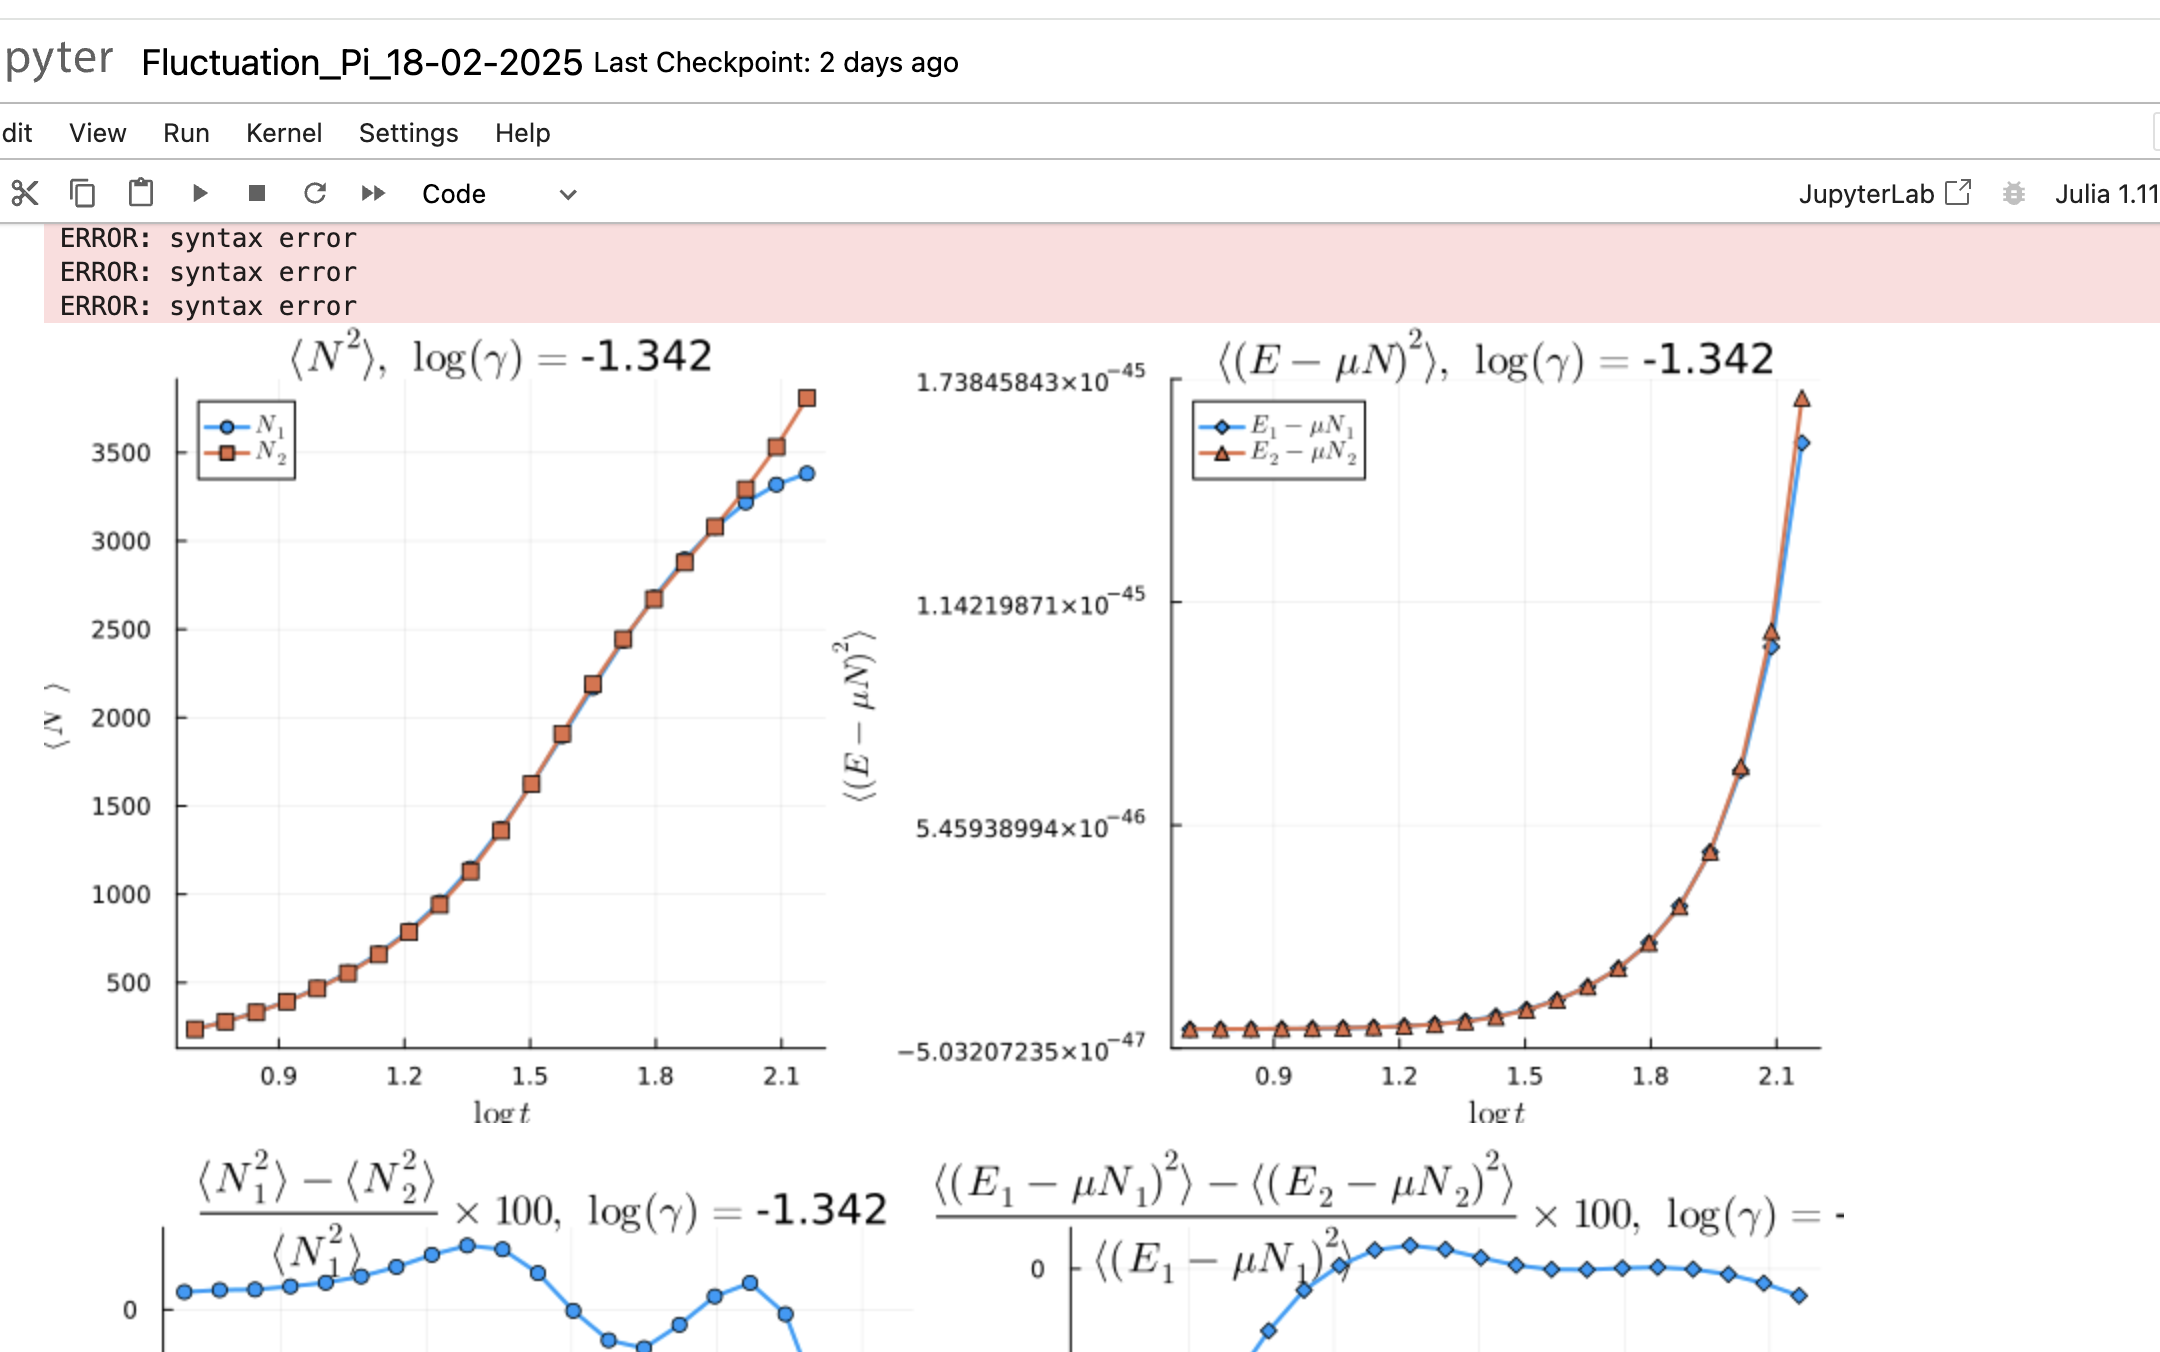
\includegraphics[width=1\textwidth]{Figures/test}

%\begin{aff}
%Donc une a l'ordre un en $\delta \theta (\operator{A}^{(0)})^{-1} %\operator{V}$ 

%\begin{eqnarray*}
%	\langle \delta \Pi ( \theta) \delta \Pi ( \theta') \rangle & = &  ( (\Pi^c_s - \Pi^c)\Pi^c/\Pi^c_s ) ( \theta ) \delta_{\theta, \theta'}/\delta \theta + \mathscr{F}(\theta , \theta' ) ,	
%\end{eqnarray*}

%avec 

%\begin{eqnarray*}
%	\mathscr{F}(\theta , \theta' ) & = & \left [ (\Pi^c_s - \Pi^c )( \theta)  +  (\Pi^c_s - \Pi^c ) ( \theta' )\right ] \frac{\Pi^c}{\Pi^c_s}(\theta)\frac{\Pi^c}{\Pi^c_s}(\theta') \frac{ \Delta( \theta'- \theta )}{ 2 \pi }\\
%	&&  - \left [ (\Pi^c_s - \Pi^c )( \theta)   (\Pi^c_s - \Pi^c ) ( \theta' )\right ] \frac{\Pi^c}{\Pi^c_s}(\theta)\frac{\Pi^c}{\Pi^c_s}(\theta')\int d\theta'' \left (   \frac{ \Pi^c/\Pi^c_s}{\Pi^c_s - \Pi^c} \right )(\theta'') \frac{\Delta(\theta''- \theta)}{2 \pi}\frac{\Delta(\theta''- \theta')}{2 \pi}  	
%\end{eqnarray*}
%\end{aff}



 









%%Les modèles mécaniques dans les dimensions espace-temps sont présentés dans cet article. Cette méthode a été suggérée pour la première fois par H. Bethe en 1931 [1] et est traditionnellement appelée l'Ansatz de Bethe. Par la suite, la méthode a été développée par Hulthen, Yang et Yang, Lieb, Sutherland, Baxter, Gaudin et d'autres (voir [2], [3], et [4]).

Nous commençons la présentation par l'Ansatz de Bethe en coordonnées, non seulement pour des raisons historiques, mais aussi en raison de sa simplicité et de sa clarté. {\color{red} La matrice de diffusion à plusieurs particules apparaît comme étant égale au produit des matrices à deux particules pour les modèles intégrables. Cette propriété de réductibilité à deux particules est d'une importance primordiale lors de la construction de la fonction d'onde de Bethe. L'une des caractéristiques importantes des modèles intégrables est qu'il n'y a pas de production multiple de particules hors des coquilles de masse. Cette propriété est étroitement liée à l'existence d'un nombre infini de lois de conservation dans de tels modèles ; cela sera expliqué dans la Partie II.}

Quatre modèles principaux, à savoir le gaz de Bose unidimensionnel, le magnétisme de Heisenberg, le modèle de Thirring massif et le modèle de Hubbard, sont considérés dans la Partie I. Les fonctions propres des hamiltoniens de ces modèles sont construites. {\color{red} L'application des conditions aux limites périodiques mène à un système d'équations pour les valeurs permises des moments. Celles-ci sont connues sous le nom d'équations de Bethe. Ce système peut également être dérivé d'un certain principe variationnel, l'action correspondante étant appelée l'action de Yang-Yang. Elle joue un rôle important dans l'étude des modèles. Les équations de Bethe sont également utiles dans la limite thermodynamique. L'énergie de l'état fondamental, la vitesse du son, etc., peuvent être calculées dans cette limite. Les excitations au-dessus de l'état fondamental, c'est-à-dire les particules physiques, sont également étudiées. Pour définir leurs caractéristiques physiques, la technique des équations de "dressing" est introduite et étudiée. La thermodynamique du modèle est expliquée en détail.}

Le matériel de cette Partie est organisé comme suit. La théorie du gaz de Bose unidimensionnel avec une interaction répulsive ponctuelle entre les particules est présentée dans le premier chapitre. La solution du magnétisme de Heisenberg X X Z dans un champ magnétique externe est donnée dans le deuxième chapitre. Le modèle quantique du champ spinor avec une auto-interaction à quatre points dans deux dimensions espace-temps est résolu dans le troisième chapitre. Cela est généralement appelé le modèle de Thirring massif, et est équivalent au modèle de sine-Gordon (dans le secteur de charge nulle). Dans le dernier chapitre de la Partie I, le modèle de Hubbard des fermions interactifs sur un réseau est brièvement abordé.


Le gaz de Bose unidimensionnel est décrit par les champs quantiques de Bose canoniques \( \Psi(x,t) \) avec les relations de commutation canoniques à temps égal :

Plus tard, l'argument \( t \) sera en règle générale omis, puisque toutes les considérations de ce chapitre s'appliquent à un instant fixé dans le temps.  
L'Hamiltonien du modèle est

où \( c \) est la constante de couplage. L'équation du mouvement correspondante est

est appelée l'équation de Schrödinger non linéaire (NS).  

Pour \( c > 0 \), l'état fondamental à température nulle est une sphère de Fermi. Seul ce cas sera considéré par la suite.  

Le vide de Fock \( |0\rangle \), défini par

est important. Il sera appelé le pseudovacuum et doit être distingué du vide physique, qui est l'état fondamental de l'Hamiltonien (la mer de Dirac). Le pseudovacuum dual \(\langle 0|\) est défini comme \(\langle 0| = |0\rangle\) et satisfait les relations

où le symbole dag (\(\dagger\)) désigne la conjugaison hermitienne. L'opérateur nombre de particules \(Q\) et l'opérateur impulsion \(P\) sont


%%\chapter*{Introduction}
%\section*{Pourquoi en 1D ?}

{\em 

Explication classique à l’aide d’un modèle chaotique : la thermalisation en 2D, illustrée par l’exemple de l’eau en ébullition, avec comme paramètres \(T\), \(E\), \(N\). Modélisation par des sphères dures et introduction du modèle ergodique : en 1D, l’intégrabilité du modèle de sphères dures dans un espace réduit entraîne un simple échange de vitesses, sans modifier la distribution des vitesses.

}

\section*{Pourquoi en 1D quantique ?}

{\em 
Le gaz de Bose unidimensionnel avec interactions ponctuelles (la version quantique de l’équation de Schrödinger non linéaire) est l’un des modèles intégrables les plus fondamentaux, pouvant être résolu par la méthode de l’Ansatz de Bethe ({ref}). Ce modèle a fait l’objet d’études approfondies ({ref}).  

Après avoir décrit le modèle de Lieb-Liniger et analysé ses asymptotiques ainsi que les théories linéarisées (Gross-Pitaevskii et Bogoliubov) dans le chapitre 1, nous poursuivons par la construction des fonctions propres de l’Hamiltonien dans un volume fini.  

Cette construction, détaillée dans le chapitre 2, met en évidence la forme explicite des fonctions propres et leur réductibilité au cas à deux particules, une caractéristique commune des modèles résolubles par l’Ansatz de Bethe. Enfin, dans la dernière section, nous imposons des conditions aux limites périodiques à %la fonction d’onde, ce qui nous conduit aux équations de Bethe pour les moments des particules, lesquelles seront introduites et analysées.
}  


%\section{Introduction au gaz de bosons unidimensionnels}



%%{\color{red}Le gaz de Bose unidimensionnel avec interaction ponctuelle des particules (la variante quantique de l'équation de Schrödinger non linéaire)} est l'un des modèles principaux et les plus importants qui peut être résolu par la méthode de l'Ansatz de Bethe [14], [15]. Ce modèle a été minutieusement étudié ([1], [5], [17], [21] et [22]). {\color{red} Nous commencerons par la construction des fonctions propres de l'Hamiltonien dans un volume fini. Les quantités intéressantes d'un point de vue physique (dans la limite thermodynamique à température nulle) sont considérées ; la thermodynamique à température finie est également étudiée en détail. Un certain nombre d'idées essentielles qui seront appliquées à d'autres modèles sont introduites.}

{\color{red} La construction des fonctions propres de l'Hamiltonien est expliquée dans la section 1. Leur forme explicite et, en particulier, la réductibilité à deux particules, sont des caractéristiques communes des modèles résolubles par la méthode de l'Ansatz de Bethe. Des conditions aux limites périodiques sont imposées à la fonction d'onde dans la section 2 ; les équations de Bethe pour les moments des particules sont introduites et analysées. Pris sous forme logarithmique, ces équations réalisent la condition d'extrémum d'un certain fonctionnel, l'action correspondante étant appelée l'action de Yang-Yang. La transition vers la limite thermodynamique est envisagée dans la section 3. Dans cette même section, l'état fondamental du gaz est construit. La densité de distribution des particules dans l'espace des moments et l'énergie de l'état fondamental sont calculées. La méthode de transition vers la limite thermodynamique décrite dans cette section est assez générale et peut être appliquée à tout modèle résoluble par l'Ansatz de Bethe. Dans la section 4, les excitations au-dessus de l'état fondamental sont construites et leurs principales caractéristiques (énergie, moment et matrice de diffusion) sont déterminées à l'aide des équations de "dressing". L'état fondamental du modèle est la mer de Dirac (également appelée sphère de Fermi).}

{\color{red} La thermodynamique du modèle est présentée dans la section 5. L'approche par intégrale fonctionnelle est présentée. Elle permet de résoudre divers problèmes à température finie. Les équations de base décrivant l'état d'équilibre thermodynamique, l'équation de Yang-Yang en étant une d'entre elles, sont dérivées dans cette section. L'équation de Yang-Yang, qui est une équation intégrale non linéaire, est analysée dans la section 6. Le théorème montrant l'existence de solutions est prouvé.} L'état d'équilibre thermodynamique avec température tendant vers zéro est étudié dans la section 7. En examinant cette limite, nous pouvons obtenir des informations plus détaillées sur l'état fondamental de l'Hamiltonien à température nulle. La limite de couplage fort (dans laquelle le modèle est équivalent au modèle de fermions libres) est discutée. Les équations intégrales sont résolues exactement dans cette limite. Les excitations au-dessus de l'état d'équilibre thermodynamique sont étudiées et leur interprétation en termes de particules est donnée. Il est important de noter que la formule à température finie et à température nulle diffèrent uniquement par la mesure d'intégration. La thermodynamique des modèles exactement résolvables est tellement particulière qu'il est possible de construire des excitations stables à température finie, voir section 8. Les corrélations thermiques sont également discutées dans la section 8. Pour les modèles exactement résolvables, elles sont également très particulières : elles peuvent être représentées sous une forme similaire à celle à température nulle. Plus tard, dans la Partie IV (Chapitres XIII-XVI), cela sera utilisé pour l'évaluation explicite des fonctions de corrélation à température (même si elles dépendent du temps). La section 9 est consacrée à l'évaluation des corrections de taille finie à température nulle. Plus tard, elles seront utilisées pour le calcul des asymptotiques de longue distance des fonctions de corrélation à l'aide de la théorie des champs conformes.

%\subsection*{Introduction}
%%\section*{Pourquoi 1D ?}

{\em Explication classique  avec la un modele chaotique : la Thermalisation en 2D avec example de l'eau qui boue avec comme parametre T , E , N ; modelisation en spher dure ; et le modele ergodique : l'integrabiliter de modele de shere dure dans un expace en 1D , echange de vitesse : distribution de vitesse inchanger}

\section*{Pourquoi 1D Quantique ?}

{\em Le gaz de Bose unidimensionnel avec interaction ponctuelle des particules (la variante quantique de l’équation de Schrödinger non linéaire) est l’un des modèles principauxet les plus importants qui peut être résolu par la méthode de l’Ansatz de Bethe ({ref}). Ce modèle a été minutieusement étudié ({ref}). Nous commencerons par la construction des fonctions propres de l’Hamiltonien dans un volume fini. La construction des fonctions propres de l’Hamiltonien est expliquée dans la section 1. Leur forme explicite et, en particulier, la réductibilité à deux particules, sont des caractéristiques communes des modèles résolubles par la méthode de l’Ansatz de Bethe. Des conditions aux limites périodiques sont imposées à la fonction d’onde dans la section 2 ; les équations deBethepour lesmoments des particules sont introduites et analysées.}

%\subsection{Description du modèle de Lieb-Liniger}
%{\color{red}Le gaz de Bose unidimensionnel avec interaction ponctuelle des particules (la variante quantique de l'équation de Schrödinger non linéaire)} est l'un des modèles principaux et les plus importants qui peut être résolu par la méthode de l'Ansatz de Bethe [14], [15]. Ce modèle a été minutieusement étudié ([1], [5], [17], [21] et [22]). {\color{red} Nous commencerons par la construction des fonctions propres de l'Hamiltonien dans un volume fini. Les quantités intéressantes d'un point de vue physique (dans la limite thermodynamique à température nulle) sont considérées ; la thermodynamique à température finie est également étudiée en détail. Un certain nombre d'idées essentielles qui seront appliquées à d'autres modèles sont introduites.}

{\color{red} La construction des fonctions propres de l'Hamiltonien est expliquée dans la section 1. Leur forme explicite et, en particulier, la réductibilité à deux particules, sont des caractéristiques communes des modèles résolubles par la méthode de l'Ansatz de Bethe. Des conditions aux limites périodiques sont imposées à la fonction d'onde dans la section 2 ; les équations de Bethe pour les moments des particules sont introduites et analysées. Pris sous forme logarithmique, ces équations réalisent la condition d'extrémum d'un certain fonctionnel, l'action correspondante étant appelée l'action de Yang-Yang. La transition vers la limite thermodynamique est envisagée dans la section 3. Dans cette même section, l'état fondamental du gaz est construit. La densité de distribution des particules dans l'espace des moments et l'énergie de l'état fondamental sont calculées. La méthode de transition vers la limite thermodynamique décrite dans cette section est assez générale et peut être appliquée à tout modèle résoluble par l'Ansatz de Bethe. Dans la section 4, les excitations au-dessus de l'état fondamental sont construites et leurs principales caractéristiques (énergie, moment et matrice de diffusion) sont déterminées à l'aide des équations de "dressing". L'état fondamental du modèle est la mer de Dirac (également appelée sphère de Fermi).}

{\color{red} La thermodynamique du modèle est présentée dans la section 5. L'approche par intégrale fonctionnelle est présentée. Elle permet de résoudre divers problèmes à température finie. Les équations de base décrivant l'état d'équilibre thermodynamique, l'équation de Yang-Yang en étant une d'entre elles, sont dérivées dans cette section. L'équation de Yang-Yang, qui est une équation intégrale non linéaire, est analysée dans la section 6. Le théorème montrant l'existence de solutions est prouvé.} L'état d'équilibre thermodynamique avec température tendant vers zéro est étudié dans la section 7. En examinant cette limite, nous pouvons obtenir des informations plus détaillées sur l'état fondamental de l'Hamiltonien à température nulle. La limite de couplage fort (dans laquelle le modèle est équivalent au modèle de fermions libres) est discutée. Les équations intégrales sont résolues exactement dans cette limite. Les excitations au-dessus de l'état d'équilibre thermodynamique sont étudiées et leur interprétation en termes de particules est donnée. Il est important de noter que la formule à température finie et à température nulle diffèrent uniquement par la mesure d'intégration. La thermodynamique des modèles exactement résolvables est tellement particulière qu'il est possible de construire des excitations stables à température finie, voir section 8. Les corrélations thermiques sont également discutées dans la section 8. Pour les modèles exactement résolvables, elles sont également très particulières : elles peuvent être représentées sous une forme similaire à celle à température nulle. Plus tard, dans la Partie IV (Chapitres XIII-XVI), cela sera utilisé pour l'évaluation explicite des fonctions de corrélation à température (même si elles dépendent du temps). La section 9 est consacrée à l'évaluation des corrections de taille finie à température nulle. Plus tard, elles seront utilisées pour le calcul des asymptotiques de longue distance des fonctions de corrélation à l'aide de la théorie des champs conformes.
%\subsection{Propriétés fondamentales et régimes asymptotiques}
%%\section{Théorie linéarisée pour le régime de quasi-condensat}
%%\subsection{Équation de Gross-Pitaevskii}
%%\subsection{Transformation de Bogoliubov pour système homogène}

%\section{Bethe Ansatz et solution exacte du modèle de Lieb-Liniger}
%%\minitoc
%\subsection{Problème à deux corps}
%\subsection{Problème à N corps}
%\subsection{Condition aux bords périodiques et équation de Bethe Ansatz}
%\begin{eqnarray*}
	L\theta_i + \sum_{j = 1}^N \Phi (\theta_i - \theta_j) = 2\pi I_i 
\end{eqnarray*}

\chapter{Relaxation et Équilibre dans les Systèmes Quantiques Intégrables : Une Approche par la Thermodynamique de Bethe}
\minitoc
\section{Équilibre thermique et ensemble de Gibbs}

%\subsection{Thermodynamique du gaz de Lieb-Liniger à température nulle}
%Dans la limite thermodynamique, le nombre de particules \( N \) et le volume 
(la longueur de la boîte) \( L \) tendent vers l'infini de sorte que leur rapport 
\( D = \frac{N}{L} \) reste fini :

\begin{eqnarray*}
	\lim_{N, L \to \infty} \frac{N}{L} = D = \mbox{const} < \infty	
\end{eqnarray*}

Considérons le système à température nulle. Rappelons que l'état 
d'énergie minimale dans le secteur avec un nombre fixe de particules 
correspond aux solutions \( j \) des équations de Bethe suivantes :

\begin{eqnarray*}
	L \theta_a + \sum_{b = 1}^N \Phi ( \theta_a - \theta_b ) & = & 2\pi I_a ,	
\end{eqnarray*}

où les nombres fermionique $I_a = a - (N+1)/2$ et $a \in \llbracket 1 , N  \rrbracket$ . Dans la limite thermodynamique, les valeurs de \( \theta_a \) se condensent (\(\theta_{a+1} - \theta_a = \mathcal{O}(1/L)\)), et remplissent l'intervalle symétrique , la mer de Dirac/sphère de Fermi  \(\llbracket-K, K\rrbracket\) où $K = \theta_N$ (ici $I_a \geqq I_b \Rightarrow \theta_a \geqq \theta_b$)

La quantité $\rho_s$ tel que (manque une intro avant ) 

\begin{eqnarray*}
	2\pi \rho_s (\theta_a) & = & \frac{2\pi}{L}\underset{\tiny \mbox{therm}}{\lim} \frac{ \vert I_{a+1} - I_{a} \vert}{ \vert \theta_{a+1} - \theta_a \vert} = \frac{2\pi}{L} \frac{ \partial I}{\partial \theta } ( \theta_a ) = 1 	+ \frac{1}{L}\sum_{b = 1}^N \Delta (\theta_a - \theta_b)
\end{eqnarray*}

représente la densité de vacances que l'on appellera densité d'état avec $I(\theta_a) = I_a$ et  $\Delta(\theta) = \Phi'(\theta)  = \frac{2c}{c^2 + \theta^2}$

Maintenant interessons nons à la densité de particules dans l'espace des moments \( \rho(\theta) \) , définie de la manière suivante :

\begin{eqnarray*}
	\rho(\theta_a)  &=  &\lim_{L \to \infty} \frac{1}{L} \frac{1}{\theta_{a+1} - \theta_a} > 0.	
\end{eqnarray*}

À l'états fondamentale tous les vacances dans $[-K , K ]$  sont occupés donc $\rho = \rho_s$. La quantité $L\rho(\theta)d\theta$ est le nombre de rapidité dans la celule $[ \theta , \theta + d \theta ] $. La quantité $L \int_{-K}^K \rho (\theta ) \, d\theta $ est le nombre de particule $N$.On remplace la somme par une intégrale :
\begin{eqnarray*}
	2\pi \rho  = 1 + \Delta \star \rho 	
\end{eqnarray*}



 





%Nous allons d'abord considérer les excitations au-dessus du vide physique dans le secteur de charge physique nulle (c'est-à-dire les excitations où le nombre de particules \( N \) dans l'état excité est identique au nombre de particules dans l'état fondamental). Nous commencerons par des conditions aux limites périodiques (2.13).

L'état fondamental est décrit par un ensemble particulier d'entiers \( n_j \), voir (2.26) et (3.2). Tous les autres ensembles de \( n_j \) (avec la contrainte que \( n_j \neq n_k \)) correspondent à des états excités. Cela constitue une description complète de tous les états excités. Ces excitations sont obtenues en supprimant un certain nombre de particules ayant des moments \( -q < \lambda < q \) de la distribution du vide (c'est-à-dire en créant des trous avec des moments \( \lambda_h \)) et en ajoutant un nombre égal de particules ayant des moments \( \lambda_p > q \).

Nous allons d'abord construire l'état dans lequel une particule de moment \( \lambda_p > q \) diffuse avec un trou de moment \( -q < \lambda_h < q \). La présence simultanée de la particule et du trou modifie les valeurs permises des moments des particules du vide : \( \lambda_j \to \tilde{\lambda}_j \), de sorte que les équations de Bethe pour les particules du vide sont réécrites comme suit.

En soustrayant cette contribution de la distribution du vide (3.2) et en tenant compte du fait que \( \lambda_j - \lambda_j' = \mathcal{O}(1/L) \) et que \( \theta( \lambda + \Delta) - \theta(\lambda) = \mathcal{O}(\Delta) \), on obtient :

En utilisant les équations (2.31), (3.5) et (3.7), on obtient :

On introduit maintenant la "fonction de décalage" \( F \) :

Dans la limite thermodynamique, on peut remplacer la somme dans (4.3) par une intégrale, ce qui donne :
Ainsi, nous sommes en mesure de décrire la polarisation du vide causée par une particule et un trou. Cela permet le calcul des grandeurs observables (énergie, momenta, et matrice de diffusion) pour les excitations au-dessus de l'état fondamental. Ces grandeurs observables sont obtenues en ajoutant les contributions de la polarisation du vide aux quantités "pures" correspondantes. Nous commençons par calculer l'énergie observable \( E \), qui est égale à l'énergie de l'état excité moins l'énergie de l'état fondamental :\\

où \( E_0(\lambda) = \lambda2 - h \). De même, on a pour le moment observable (le moment "pur" est simplement égal à $\lambda$) :

Toutes les excitations dans le secteur à charge nulle peuvent être construites comme un état de diffusion constitué de nombres égaux de particules et de trous. L'énergie et le moment de ces excitations sont égaux à la somme des énergies et des moments des particules et des trous individuels. L'excitation à une particule et un trou construite ci-dessus est un état à deux corps. Dans l'ensemble canonique grand, nous pouvons changer le nombre de particules. Construisons une excitation à une particule avec énergie :

et le moment \( k(p) \) égal à :

(voir (3.7)). Il s'agit d'une excitation topologique (nous devons changer les conditions aux frontières en antipériodiques). La valeur \( \lambda_p \) doit être en dehors de la sphère de Fermi, \( |\lambda_p| > q \), \( \text{Im} \, \lambda_p = 0 \). On peut également construire une autre excitation topologique (trou élémentaire) avec une énergie égale à \( -e(h) \) et un moment égal à :

où \( -q < \lambda < g \). Cela montre que les états excités dans le secteur neutre construits ci-dessus sont constitués de deux excitations élémentaires (comparer les formules (4.19) et (4.20) avec (4.16)). Pour construire ces excitations topologiques, il faut changer les conditions aux frontières pour qu'elles soient antipériodiques lors de l'introduction d'une excitation.

Cette excitation topologique a une nature fermionique. Pour les bosons implacables, cela est explicitement montré dans l'Appendice 1. Ainsi, nous allons introduire une autre particule dans l'état fondamental et changer les conditions aux frontières.
Dans l'état excité, il y a \( N + 1 \) particules avec des moments \( \tilde{\lambda}_j; j = 1, \dots, N + 1 \). Les équations de Bethe correspondantes sont :

L'état excité est caractérisé par l'ensemble de \( N + 1 \) nombres \( \{ n_j, j = 1, \dots, N + 1 \} \); les \( N \) premiers nombres correspondent à l'état fondamental (2.26). Notons \( \lambda_{N+1} \) par \( \lambda_p \). Il est commode d'introduire une fonction de décalage \( F \) similaire à celle de (4.4) :

Dans la limite thermodynamique, la fonction de décalage satisfait l'équation intégrale suivante :

où \( |\lambda_p | > q \). La fonction \( F(\mu|\lambda) \) est définie pour \( |\mu| < q \); cependant, à l'aide de l'équation (4.25), \( F \) peut être prolongée analytiquement sur tout l'axe réel.

Avec l'aide de la fonction de décalage, nous pouvons calculer les quantités observables dans la limite thermodynamique (énergie, moment et matrice de diffusion). La fonction de décalage décrit le nuage de particules virtuelles qui entoure la particule \( p \) ou, en d'autres termes, la polarisation du vide due à la particule nue \( p \). Des calculs similaires à ceux du début de cette section montrent que l'énergie d'une particule est \( \varepsilon(\lambda_p) \) (voir (4.9)) et que le moment est donné par (4.19).

Une excitation de "trou" peut être traitée de manière similaire. Le nombre de particules dans cette excitation est égal à \( N - 1 \) et la charge observable est égale à \( -1 \). La fonction d'onde \( X_N \) doit à nouveau être antiperiodique. Cet état est caractérisé par l'ensemble de nombres entiers \( \{n_j\} \) obtenu en éliminant un nombre de l'ensemble du vide. La fonction de décalage satisfait l'équation

où \( | \lambda_h | < q \) est le moment de la particule nue du trou. Avec l'aide de cette fonction, l'énergie et le moment peuvent être obtenus :


Cette fonction peut être remplacée par \( -k_h(\lambda_h) \) trouvé dans (4.19).
Les excitations arbitraires sont construites à partir de plusieurs particules et trous.
L'énergie et le moment de telles excitations sont simplement la somme des contributions des excitations élémentaires individuelles. Ainsi, l'énergie et le moment sont donnés par :


La matrice de diffusion à plusieurs corps est simplement le produit des matrices de diffusion à deux corps. D'abord, la matrice de diffusion pour deux particules sera évaluée. L'ajout de deux particules (\( \lambda_2 > \lambda_1 > q \)) au vide déplace les valeurs des moments des particules du vide : \( \lambda_j \rightarrow \tilde{\tilde{\lambda}}_j \) (pour \( j = 1, \ldots, N \)). La fonction de décalage

est égale à la somme des fonctions de décalage à une particule données par (4.25) :

Maintenant, considérons la matrice de diffusion de deux particules possédant des moments \( \lambda_1 \) et \( \lambda_2 \) avec \( \lambda_2 > \lambda_1 > q \), comme ci-dessus. Dans ce cas, la matrice de diffusion est simplement un facteur numérique de module unitaire ; ainsi, elle peut être écrite comme


Le phase \( \delta \) est réelle et est donnée par


où \( \varphi_2 \) est la phase complète que la deuxième particule acquiert lorsqu'elle traverse l'ensemble de la boîte dans le cas où la première particule est absente :

La phase \( \varphi_{21} \) est la phase complète que la deuxième particule acquiert lorsqu'elle traverse l'ensemble de la boîte en présence de la première :

En utilisant les équations (4.34) et (4.35), la phase de diffusion est donnée par

En changeant la somme en une intégrale dans la limite thermodynamique et en utilisant (4.31), on obtient

et à partir de (4.25)

Ainsi, la phase de diffusion satisfait l'équation intégrale suivante :

Nous avons démontré que les excitations physiques au-dessus de la mer de Dirac sont obtenues à partir des excitations "nues" au-dessus du vide de Fock \( |0\rangle \) (qui sont décrites par les fonctions d'onde de Bethe) à travers les équations de "dressing". Ces équations linéaires intégrales de dressing sont des équations universelles. Pour le voir, il suffit de comparer les équations de dressing pour l'énergie (4.9), la phase de diffusion (4.39) et la densité (3.7). Les équations de dressing sont également très utiles pour l'étude des fonctions de corrélation et des corrections de taille finie, comme nous le verrons dans les sections suivantes.

La diffusion de deux trous ayant des momenta nues \( \lambda_1 \) et \( \lambda_2 \), avec \( -q \leq \lambda_{1, 2} \leq q \), est également égale à \( \exp\left(i \varphi(\lambda_2, \lambda_1)\right) \) où \( \varphi \) est défini par (4.39). La matrice de diffusion de la particule \( \lambda_p \) avec le trou \( \lambda_h \) est égale à


La matrice de diffusion de plusieurs particules est égale au produit des matrices de diffusion à deux particules.

Il convient également de mentionner que les structures d'excitation d'autres modèles (antiferromagnétique XXZ de Heisenberg et modèle de sine-Gordon) sont très similaires. L'énergie, le moment et la matrice de diffusion sont évalués de la même manière.








\subsection{Physique statistique de l’ensemble de Gibbs}
%%Considérons l'ensemble canonique et calculons la fonction de partition $Z$ du modèle.

Ici, $H$ est le hamiltonien donné par (1.2) et $T$ est la température.  
L'énergie libre $F$ est donnée par (5.1). Rappelons que nous étudions  
la limite thermodynamique ($L \to \infty, N \to \infty$) tout en conservant  
la densité du gaz fixe :

Dans la limite thermodynamique, les lacunes, les particules et les trous  
(ceux définis dans la section 2, voir (2.29), (2.30)) ont des densités de  
distribution finies $\rho_t(\lambda)$, $\rho_p(\lambda)$ et $\rho_h(\lambda)$  
dans l'espace des moments, qui sont définies comme suit :

Le nombre de lacunes est simplement la somme du nombre de particules  
et de trous :

Par lacunes, nous entendons les positions potentielles, dans l'espace des moments,  
qui peuvent être occupées par des particules ou des trous. Dans la limite thermodynamique,  
la somme dans l'équation (2.31) se transforme en une intégrale impliquant la densité $\rho_p(\lambda)$  
et on a :

Il convient de souligner que nous passons maintenant d'une description microscopique  
du modèle (à l'aide de l'ensemble $\{n_j\}$) à une description macroscopique  
en termes de densités $\rho_p$, $\rho_h$ et $\rho_t$.  
La situation macroscopique donnée, décrite par des valeurs fixées de $\rho_p$, $\rho_h$ et $\rho_t$,  
correspond à de nombreux ensembles d'états microscopiques (les ensembles de nombres $\{n_j\}$).  
En effet, il existe de nombreuses façons de placer $L \rho_p(\lambda) d\lambda$ particules  
dans $L \rho_t(\lambda) d\lambda$ lacunes. Le nombre de possibilités est donné par :

Ce nombre est grand dans la limite thermodynamique.  
En utilisant la formule de Stirling pour l'asymptotique du factoriel, on obtient :

Plus tard, nous verrons que l'énergie et les autres observables du système 
ne dépendent que des variables macroscopiques \( \rho_p \) et \( \rho_h \). La quantité

est l'entropie. Passons maintenant à la fonction de partition (5.1). Elle peut être 
représentée sous la forme

où \( E_N = \sum \lambda^2 \} \) et les moments \( \lambda_j \) sont les solutions des équations de Bethe (2.13). 
Nous allons considérer la thermodynamique du gaz qui est au repos dans son ensemble, 
ainsi l'impulsion totale \( P_N \) (1.29) est égale à zéro ; cela signifie que \( \sum n_j = 0 \). 
En introduisant de nouvelles variables \( n_{j+1 , j} = n_{j+1} - n_j \), nous pouvons réécrire (5.11) :

Dans la limite thermodynamique, l'énergie d'un état





%Dans ce chapitre, nous nous intéressons aux fluctuations de la distribution de rapidité \( \delta \rho \) autour d'une distribution de référence \( \rho^c \), qui maximise la contribution à la fonction de partition des états, exprimée comme une fonctionnelle de la distribution \( \rho \) : 

La fonction de partition des états, s'exprime comme une fonctionnelle de la distribution \( \rho \) : 

\begin{eqnarray*}
	\Xi & = & \sum_\rho \exp \left( -\mathcal{A}(\rho) \right).
\end{eqnarray*}  

Dans la section {\em \bf Entropie de Yang-Yang} (\ref{??}), l'action \( \mathcal{A}(\rho) \) s'écrit sous la forme :  

\begin{eqnarray*}
	\mathcal{A}(\rho) & \doteq & - L\mathcal{S}_{YY}(\rho) + L\int f(\theta) \rho (\theta) \, d\theta,		
\end{eqnarray*}  

où \( \mathcal{S}_{YY} \) est la fonctionnelle d'entropie de Yang-Yang, définie dans (\ref{??}), et \( f \) est la fonction paramétrant les charges, introduite dans (\ref{??}).  

Dans cette même section {\em \bf Entropie de Yang-Yang} (\ref{??}), nous avons établi un lien entre \( f \) et distribution de référence \( \rho^c \), qui maximise la contribution à la fonction de partition des états .\\

On veux tester si nos experience est décrit pas un GGE. Pour cela nous nous intéressons aux fluctuations de la distribution de rapidité \( \delta \rho \) autour \( \rho^c \).

%Nous poursuivons à présent avec cette définition de l'action de classe $\mathcal{C}^2$ et admetant une distribution critique $\rho^c$ tel que sa différentielle en ce point critique soit nulle $d\mathcal{A}_{\rho^c} = 0 $ (\ref{??}) de sorte que d'aprés la formule de Taylor-Youg %afin de déterminer les fluctuations autour de \( \Pi^c \). Pour cela, nous réécrivons l'action sous la forme :  

Nous poursuivons à présent avec cette définition de l'action de classe $\mathcal{C}^2$ et admetant une distribution critique $\rho^c$ tel que sa différentielle en ce point critique soit nulle $d\mathcal{A}_{\rho^c} = 0 $ (\ref{??}) de sorte que d'aprés la formule de Taylor-Youg %afin de déterminer les fluctuations autour de \( \Pi^c \). Pour cela, nous réécrivons l'action sous la forme :  

\begin{eqnarray*}  
	\mathcal{A}(\rho^c + \delta \rho) & \underset{ \delta \rho \to 0 }{=} & \mathcal{A}(\rho^c)  + \frac{1}{2} \left. \frac{\delta^2 \mathcal{A}}{\delta \rho^2} \right|_{\rho^c} (\delta \rho) + \mathcal{O}((\delta \rho)^3),  
\end{eqnarray*}  

une expression quadratique pour l'action à l'ordre dominant en \( \delta \Pi \) avec $\left. \frac{\delta^2 \mathcal{A}}{\delta \rho^2} \right|_{\rho^c}$ la forme quadratique définie positive (Fig (\ref{fig.fluctu.A})).

\begin{figure}[H]
	\centering 
	\begin{tikzpicture}
		\begin{scope}[shift={(0,0)}]
			\begin{scope}[transform canvas={scale=0.6}]
				% Définition des couleurs avec les codes HTML
\definecolor{colorOne}{HTML}{443E46}
\definecolor{colorTwo}{HTML}{F6DEB8}
\definecolor{colorThree}{HTML}{908CA4}
\definecolor{colorFour}{HTML}{57659E}
\definecolor{colorFive}{HTML}{C57284}
\definecolor{colorSix}{HTML}{FF5B69}

% Raccourcis pour les couleurs
\def\colorOne{colorOne}
\def\colorTwo{colorTwo}
\def\colorThree{colorThree}
\def\colorFour{colorFour}
\def\colorFive{colorFive}
\def\colorSix{colorSix}

\def\colorslide{blue!50!black}



\begin{scope}
	% Tracer une courbe lisse entre des points
	\draw[shift={(0,0)} ,\colorOne]
		(-1 , 0 ) edge [thick,line width=0.8ex , ->,>=triangle 45  , \colorOne] node [pos = 1 , below ]{\huge$\rho$}( 5  , 0 )
	;
	\draw[shift={(0,0)}, color=\colorOne]
		(0, -1.0 ) edge [thick,line width=0.8ex , ->,>=triangle 45  ]node [pos=0.9,left=0.2cm ]{\huge$\mathcal{A}(\rho)$}( 0  , 5 )
	;
	\draw[]
		(2.5, 0.12 ) edge [thick,line width=0.8ex ,\colorThree ]node [pos=1,below  ]{\huge$\rho^c$} (2.5, -0.12 )	
	;
	
	\draw[]
		(2.5, -0.12 ) edge [thick,line width=0.4ex , dashed, \colorThree ] (2.5, 5.5 )
		(1.5, 1 ) edge [thick,line width=0.4ex , <->,>=triangle 45  , \colorThree ] (3.5, 1 )
		(-0.3,1) edge [thick,line width=0.4ex  , \colorThree ] node [pos=0,left ]{\huge$\mathcal{A}(\rho^c)$} (0.3, 1 )	
	;
    \draw[thick, line width=0.8ex , \colorFour] plot[smooth, tension=0.7] coordinates {
        (1, 5) (1.6 , 3 ) (2.5, 1) (3.5 , 3 )  (4, 5)
    };		
	
\end{scope}

	
			
			\end{scope}
			
			\draw[color = red , scale = 0.5 , draw = none  ] (-2 , -1) rectangle (5, 6) ; 	
		\end{scope}
		
		\begin{scope}[shift={(19,-1)}]
			\begin{scope}[transform canvas={scale=0.6}]
				% Définition des couleurs avec les codes HTML
\definecolor{colorOne}{HTML}{443E46}
\definecolor{colorTwo}{HTML}{F6DEB8}
\definecolor{colorThree}{HTML}{908CA4}
\definecolor{colorFour}{HTML}{57659E}
\definecolor{colorFive}{HTML}{C57284}
\definecolor{colorSix}{HTML}{FF5B69}

% Raccourcis pour les couleurs
\def\colorOne{colorOne}
\def\colorTwo{colorTwo}
\def\colorThree{colorThree}
\def\colorFour{colorFour}
\def\colorFive{colorFive}
\def\colorSix{colorSix}

\def\colorslide{blue!50!black}

\def\Occupation{
	\def\traitx{0.3}
	\def\traity{0.5}
	\draw[shift={(0,0)}]
		(-13.5 , 0 ) edge [thick,line width=0.8ex ]( -3.2  , 0 )
		( -3.2 - \traitx  , 0 - \traity ) edge [thick,line width=0.8ex ]( -3.2 + \traitx  , 0 + \traity  )
		( -2.8 - \traitx  , 0 - \traity ) edge [thick,line width=0.8ex ]( -2.8 + \traitx  , 0 + \traity  )
		(-2.8 , 0 ) edge [thick,line width=0.8ex ](2.8  , 0 )
		( 2.8 - \traitx  , 0 - \traity ) edge [thick,line width=0.8ex ]( 2.8 + \traitx  , 0 + \traity  )
		( 3.2 - \traitx  , 0 - \traity ) edge [thick,line width=0.8ex ]( 3.2 + \traitx  , 0 + \traity  )
		(3.2, 0 ) edge [thick,line width=0.8ex,->,>=triangle 45 , color = black ]node [pos=1.01,below  ]{\huge$\theta$}	( 13  , 0 )
	;
	\draw[shift={(0,0)}, color=\colorOne]
		(-10.5 , -1.5 ) edge [thick,line width=0.8ex , ->,>=triangle 45  ]( -10.5  , 4.5 )
	;
		
	\foreach \r in {1 , ... , 3 } {
%		\draw[
%		decoration={
%		markings,
%    	mark connection node=my node,
%    	mark=at position 0 with{\node [blue,transform shape] (my node) {\large \r};}},
%		color=gray, thick, 
%		line width=0.5ex] decorate { 
%            (-11.0, \r) -- (-10.1, \r )}
%        ;
        \draw[
			color=\colorOne,
			] 
            (-11.0, \r) edge[color=\colorThree , thick,line width=0.5ex] node [pos=-0.5 ]{\large\color{\colorFour} $\frac{\r}{\delta \theta}$ } (-10.3, \r )
        	;
	
	}
	

	
	% Graduation abcsisse 
	% Définitions des listes
% Definitions of the lists
\def\listetuple{-9/\theta_{1}, -8/\theta_{2} , -5/\theta_{3} , -2/\theta_{a-1} , 0/\theta_{a} , 1/\theta_{a+1} , 2/\theta_{a+2} ,  5/\theta_{N-4} , 7/\theta_{N-3},8/\theta_{N-1},9/\theta_{N} }
\def\listetrais{-12 , -11, -10, -9 , -8 , -7 ,  -6 , -5, -4.5,-4, -2 , -1, 0 , 0.5, 1, 2, 4 , 5 ,  6 , 7 , 8 ,8.5, 9 ,  10 , 11, 12 }

% Loop over listetrais
\foreach \r in \listetrais {
    % Initialize found variable to zero
    % Initialize found variable to zero
    %\pgfmathsetmacro\found{0}
    \global\def\found{0}
    \xdef\nomtheta{}
    
    % Check if \r is in listetuple
    \foreach \x/\y in \listetuple { 
        \ifdim \r pt=\x pt % If \r matches any \x in listetuple
            \global\def\found{1} ;
            \xdef\nomtheta{\y} % Set \nomtheta to the corresponding \y
            %\pgfmathsetmacro\found{1} % Set found to 1            
            %\global\pgfmathsetmacro\found{1}
        \fi
    }
    
    %\node [circle, draw, red] (A) at (\r, 2) {\found , $\nomtheta$};
    
    % Draw the line and display \nomtheta if found
    \ifnum\found=1
        \draw[color=\colorOne, thick, line width=0.5ex] 
            (\r, -0.3) -- (\r, 0.3) node[red , pos=-0.5] {\large $\nomtheta$};
         \filldraw[line width=0.5ex, color=\colorSix, outer color=\colorSix, inner color=\colorSix] 
            (\r, 0) circle (4pt);
    \else 
        % Draw without \nomtheta and add a blue circle if not found
        \draw[color=\colorOne, thick, line width=0.5ex] 
            (\r, -0.3) -- (\r, 0.3);
        \filldraw[line width=0.5ex, color=\colorSix, outer color=\colorTwo, inner color=\colorTwo] 
            (\r, 0) circle (4pt); 
    \fi
}

\def\listetrais{-9.5/\theta_{i-1}/2/3, -6.5/\theta_{i}/1/4  ,   -1.5/\theta_{j}/2/4 , 1.5/\theta_{j+1}/-1/3 , 3.5/\theta_{\ell-1}/1/3 , 6.5/\theta_{\ell}/3/4 , 9.5/\theta(\theta_{\ell+1})/-1/3 };



\foreach \r/\nomx/\y/\ys in \listetrais {
	\draw[
		decoration={
		markings,
    	mark connection node=my node,
    	mark=at position .5 with{\node [blue,transform shape] (my node) {\large \color{\colorFour} $\nomx$};}},
		color=\colorThree , thick, 
		line width=0.5ex] decorate { 
            (\r, 0.12) -- (\r, -1.2)}
        ;
     
     \ifdim \y pt > -1 pt 
     	\draw[
			decoration={
			markings,
    		mark connection node=my node,
    		mark=at position .5 with{\node [blue,transform shape] (my node) {\large \color{\colorFour} $\Pi(\nomx) $};}},
			color=\colorThree, thick, 
			line width=0.5ex] decorate { 
            (\r, \y) -- (\r +3, \y)}
        ;
        \draw[
			decoration={
			markings,
    		mark connection node=my node,
    		mark=at position .5 with{\node [blue,transform shape] (my node) {\large \color{\colorFive} $\Pi_s(\nomx) $};}},
			color=\colorFive, thick, 
			line width=0.5ex] decorate { 
            (\r, \ys) -- (\r +3, \ys)}
        ;
     \fi 
     \ifdim \r pt= -1.5 pt
     	\draw[
     		decoration={
			markings,
    		mark connection node=my node,
    		mark=at position .5 with{\node [blue,transform shape] (my node) {\large \color{\colorFour}  $\delta \theta $};},
    		%mark=at position 0.1  with {\arrow[blue, line width=0.5ex]{<}},
    		%mark=at position 1  with {\arrow[blue, line width=0.5ex]{>}}
    		},
        	color=\colorThree,
        	thick,
        	line width=0.5ex,
        	%arrows={Computer Modern Rightarrow[line cap=round]-Computer Modern Rightarrow[line cap=round]}
   			](\r, -1.2) edge[arrows={Computer Modern Rightarrow[line cap=round]-}] (\r + 0.4, -1.2)decorate {
    		(\r, -1.2) -- (\r + 3, -1.2)}(\r + 2, -1.2) edge[arrows={-Computer Modern Rightarrow[line cap=round]}] (\r + 3, -1.2)
    		;
    \fi
			
	
}


			
}


\begin{scope}
	%\draw[help lines , width=1.5ex] (-8,-3) grid (8,3);\draw[help lines ,width=0.5ex , opacity = 0.5] (-3,-3) grid[step=0.1] (3,3));
	
	%\draw[help lines] 
	%	(-3,-3) edge[width=1.5ex] grid (3,3)	
	%	(-3,-3) edge[width=0.5ex , opacity = 0.5] grid (3,3)	
	%;
	\begin{scope}[shift={(0,1)},rotate=0,opacity=1,color=black]
		\Occupation	
		
		%\node[anchor=east, font=\bfseries] at (-11, 0) {\color{red}\large (T = 0 )} ;	
	\end{scope}
	
	
	
	
	\begin{scope}[shift={(-10.5,7)},rotate=0,opacity=1,color=black]
	
	\begin{scope}[shift={(-0,0)},rotate=0,opacity=1,color=black]
	
		\draw[shift={(0,0)} ,line width=1ex,rounded corners = 1ex,color=\colorOne , opacity =1 ,fill=\colorOne!00 , pattern={north east lines} , pattern color=\colorOne!00 ]
			(0 , -1 ) rectangle (5,1)
		;
		

		\begin{scope}[shift={(0.5,0.5)}]
			\draw[color=\colorOne, thick, line width=0.5ex] 
            (0, -0.3) -- (0, 0.3) ;
            \filldraw[line width=0.5ex, color=\colorSix, outer color=\colorSix, inner color=\colorSix] 
            (0, 0) circle (4pt);
            
            \node[anchor=west, font=\bfseries] at (0.2, 0) {\color{\colorSix}\large : quasi-particule};
		\end{scope}
		
		\begin{scope}[shift={(0.5,-0.5)}]
			\draw[color=\colorOne, thick, line width=0.5ex] 
            (0, -0.3) -- (0, 0.3) ;
            \filldraw[line width=0.5ex, color=\colorSix, outer color=\colorTwo, inner color=\colorTwo] 
            (0, 0) circle (4pt);
            
            \node[anchor=west, font=\bfseries] at (0.2, 0) {\color{\colorSix}\large : hole};
		\end{scope}

	\end{scope}
	
	\begin{scope}[shift={(6,0)},rotate=0,opacity=1,color=black]	
		
		\draw[shift={(0,0)} ,line width=1ex,rounded corners = 1ex,color=\colorOne , opacity =1 ,fill=\colorOne!00 , pattern={north east lines} , pattern color=\colorOne!00 ]
			(0 , -1 ) rectangle (7.5,1)
		;
		
		\node[anchor=west] at (0.5, 0.5) {\color{\colorFour}\large $\Pi$ };\node[anchor=west, font=\bfseries] at (1, 0.5) {\color{\colorFour}\large : quasi-particule distribution};
		
		\node[anchor=west] at (0.5, -0.5) {\color{\colorFour}\large $\Pi_h$ };\node[anchor=west, font=\bfseries] at (1, -0.5) {\color{\colorFour}\large  : hole distribution};
		
	\end{scope}
	
	\begin{scope}[shift={(14.5,0)},rotate=0,opacity=1,color=black]	
		
		\draw[shift={(0,0)} ,line width=1ex,rounded corners = 1ex,color=\colorOne , opacity =1 ,fill=\colorOne!00 , pattern={north east lines} , pattern color=\colorOne!00 ]
			(0 , -0.5 ) rectangle (7.0,0.5)
		;
		
		\node[anchor=west] at (0.2, 0) {\color{\colorFour}\large ${\color{\colorFive}\Pi_s} = \Pi + \Pi_h $ } node[anchor=west , font=\bfseries] at (3.1 , 0 )  {\color{\colorFour}\large {\color{\colorFive} : density of states}};
		
	\end{scope}
	
	
	\end{scope}


		
	
\end{scope}

	
			
			\end{scope}
			\begin{scope}[scale=1]
				\draw[color = red , scale = 1 , draw = none  ] (-1 , -1) rectangle (5, 5) ; 
			\end{scope}	
		\end{scope}

		
				
			
	\end{tikzpicture}	
	\captionsetup{skip=10pt} % Ajoute de l’espace après la légende
	\label{fig.fluctu.A}
\end{figure}


On discrétise l'axe des rapidités en  petite cellule de rapidité $[\theta, \theta+\delta\theta]$, qui contient $L\rho(\theta) \delta \theta$ rapidités. 
	



Avec ces petites tranches, la forme quadratique s’écrit :

\begin{eqnarray*}
    \left. \frac{\delta^2 \mathcal{A}}{{\delta \rho}^2} \right|_{\rho^c}(\delta \rho ) &=&  \sum_{a,b \mid \text{tranche}}  
    \delta \rho(\theta_a)  \frac{\partial^2 \mathcal{A}}{\partial \delta \rho(\theta_a) \partial \delta \rho(\theta_b) } (\rho^c)  \delta \rho(\theta_b).
\end{eqnarray*}
Les fluctuations s’écrivent donc :

\begin{eqnarray*}
    \langle \delta \rho ( \theta) \delta \rho ( \theta') \rangle &=&  
    \frac{ \int d\delta \rho \, \delta \rho(\theta) \delta \rho ( \theta') 
    \exp \left( - \frac{1}{2} \sum_{a,b \mid \text{tranche}}  
    \delta \rho(\theta_a) \frac{\partial^2 \mathcal{A}}{\partial \delta \rho(\theta_a) \partial \delta \rho(\theta_b) } (\rho^c)  \delta \rho(\theta_b) \right) }
    { \int d\delta \Pi  
    \exp \left( - \frac{1}{2} \sum_{a,b \mid \text{tranche}}  
    \delta \rho(\theta_a) \frac{\partial^2 \mathcal{A}}{\partial \delta \rho(\theta_a) \partial \delta \rho(\theta_b) } (\rho^c)  \delta \rho(\theta_b) \right) } \\
    &=& \left( \mathbf{A}^{-1} \right)_{\theta , \theta'}
\end{eqnarray*}


\begin{aff}

\begin{eqnarray*}
	\langle \delta \rho ( \theta) \delta \rho ( \theta') \rangle &=& 	\left( \mathbf{A}^{-1} \right)_{\theta , \theta'}
\end{eqnarray*}

	
avec la  {\em matrice hessienne} $\mathbf{A}_{\theta , \theta'} \equiv \frac{\partial^2 \mathcal{A}}{\partial \delta \rho(\theta) \partial \delta \rho(\theta') }(\rho^c)$, au point critique/ qui maximise la probabilité  $\rho^c=\rho^c_s \nu^c $, s'écrit

\begin{eqnarray*}
	\operator{A} & = & \operator{A}^{(0)} + \delta \theta \operator{V}
\end{eqnarray*}

avec 

\begin{eqnarray*}
	A^{(0)}_{\theta , \theta'}  & = &  L\delta \theta \left ( \frac{ 1}{\rho^c_s ( 1  - \nu^c ) \nu^c } \right )(\theta)    \delta({\theta - \theta '})	,\\
	V_{\theta , \theta'}  &= & L \delta \theta \left \{ - \left [ \left ( \frac{1}{\rho^c_s( 1 - \nu^c) } \right ) ( \theta)  +  \left ( \frac{1}{\rho^c_s( 1 - \nu^c) } \right ) ( \theta' )\right ] \frac{ \Delta( \theta'- \theta )}{ 2 \pi } + \int d\theta''  \left ( \frac{\nu^c}{\rho^c_s( 1 - \nu^c) } \right )(\theta'') \frac{\Delta(\theta''- \theta)}{2 \pi}\frac{\Delta(\theta''- \theta')}{2 \pi}   \right \} 	
\end{eqnarray*}

\end{aff}

\subsection{Testes}

\begin{eqnarray*}
	\Delta_{\operator{\mathcal{N}}}^2  & = &  \frac{1}{\beta} \left . \frac{\partial \langle \operator{\mathcal{N}} \rangle}{\partial \mu} \right )_T \\
	\Delta_{\operator{\mathcal{E}}-\mu \operator{\mathcal{N}}}^2  & = &  - \left . \frac{\partial \langle \operator{\mathcal{E}}-\mu \operator{\mathcal{N}} \rangle}{\partial \beta} \right )_\mu 
\end{eqnarray*}

et 

\begin{eqnarray*}
	\Delta_{\operator{\mathcal{N}}}^2  &= & L^2 \int d\theta_a \int d \theta_b \, \langle \delta \rho(\theta_a) \delta \rho(\theta_b) \rangle \\
	\Delta_{\operator{\mathcal{E}}-\mu \operator{\mathcal{N}}}^2  & = & L^2 \int d\theta_a \int d \theta_b \, \left ( - \mu + \frac{1}2 m \theta_a^2  \right  )\left ( - \mu + \frac{1}2 m \theta_b^2  \right  )  \langle \delta \rho(\theta_a) \delta \rho(\theta_b) \rangle
\end{eqnarray*}

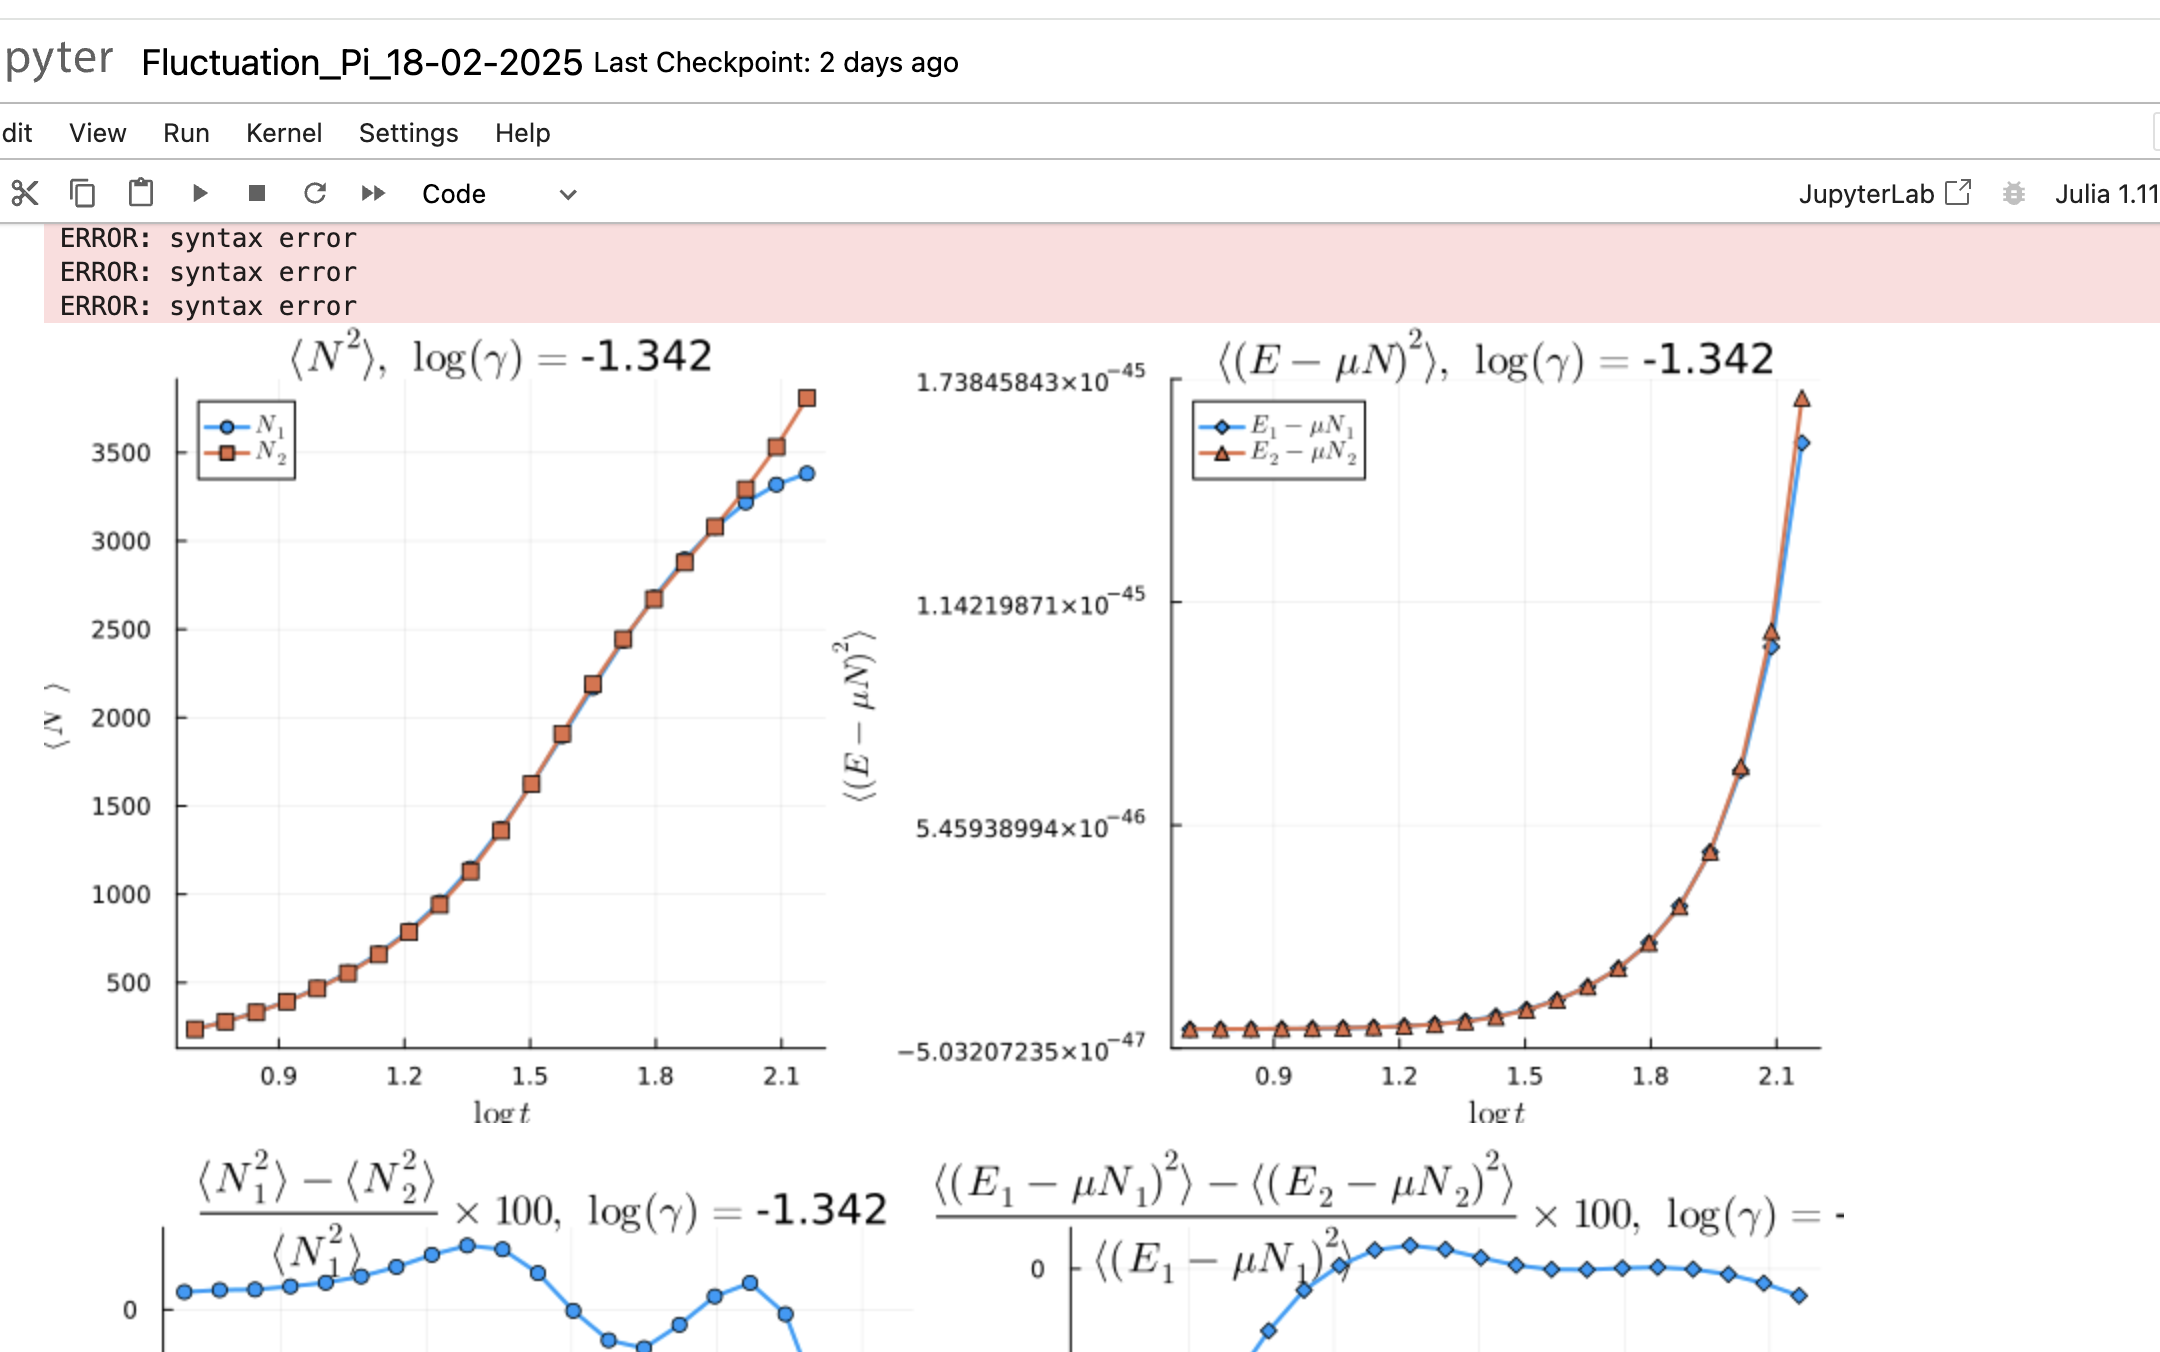
\includegraphics[width=1\textwidth]{Figures/test}

%\begin{aff}
%Donc une a l'ordre un en $\delta \theta (\operator{A}^{(0)})^{-1} %\operator{V}$ 

%\begin{eqnarray*}
%	\langle \delta \Pi ( \theta) \delta \Pi ( \theta') \rangle & = &  ( (\Pi^c_s - \Pi^c)\Pi^c/\Pi^c_s ) ( \theta ) \delta_{\theta, \theta'}/\delta \theta + \mathscr{F}(\theta , \theta' ) ,	
%\end{eqnarray*}

%avec 

%\begin{eqnarray*}
%	\mathscr{F}(\theta , \theta' ) & = & \left [ (\Pi^c_s - \Pi^c )( \theta)  +  (\Pi^c_s - \Pi^c ) ( \theta' )\right ] \frac{\Pi^c}{\Pi^c_s}(\theta)\frac{\Pi^c}{\Pi^c_s}(\theta') \frac{ \Delta( \theta'- \theta )}{ 2 \pi }\\
%	&&  - \left [ (\Pi^c_s - \Pi^c )( \theta)   (\Pi^c_s - \Pi^c ) ( \theta' )\right ] \frac{\Pi^c}{\Pi^c_s}(\theta)\frac{\Pi^c}{\Pi^c_s}(\theta')\int d\theta'' \left (   \frac{ \Pi^c/\Pi^c_s}{\Pi^c_s - \Pi^c} \right )(\theta'') \frac{\Delta(\theta''- \theta)}{2 \pi}\frac{\Delta(\theta''- \theta')}{2 \pi}  	
%\end{eqnarray*}
%\end{aff}



 








%%\section{Chaos quantique et brisure de l’intégrabilité}
\subsection{Entropie de Yang-Yang et principe de maximisation}

\section{Équilibre non thermique et ensemble de Gibbs généralisé}

\subsection{Intégrabilité et charges conservées}
\subsection{Dynamique hors équilibre et relaxation des systèmes isolés}
\subsection{Physique statistique appliquée aux systèmes intégrables}
%Dans ce chapitre, nous nous intéressons aux fluctuations de la distribution de rapidité \( \delta \rho \) autour d'une distribution de référence \( \rho^c \), qui maximise la contribution à la fonction de partition des états, exprimée comme une fonctionnelle de la distribution \( \rho \) : 

La fonction de partition des états, s'exprime comme une fonctionnelle de la distribution \( \rho \) : 

\begin{eqnarray*}
	\Xi & = & \sum_\rho \exp \left( -\mathcal{A}(\rho) \right).
\end{eqnarray*}  

Dans la section {\em \bf Entropie de Yang-Yang} (\ref{??}), l'action \( \mathcal{A}(\rho) \) s'écrit sous la forme :  

\begin{eqnarray*}
	\mathcal{A}(\rho) & \doteq & - L\mathcal{S}_{YY}(\rho) + L\int f(\theta) \rho (\theta) \, d\theta,		
\end{eqnarray*}  

où \( \mathcal{S}_{YY} \) est la fonctionnelle d'entropie de Yang-Yang, définie dans (\ref{??}), et \( f \) est la fonction paramétrant les charges, introduite dans (\ref{??}).  

Dans cette même section {\em \bf Entropie de Yang-Yang} (\ref{??}), nous avons établi un lien entre \( f \) et distribution de référence \( \rho^c \), qui maximise la contribution à la fonction de partition des états .\\

On veux tester si nos experience est décrit pas un GGE. Pour cela nous nous intéressons aux fluctuations de la distribution de rapidité \( \delta \rho \) autour \( \rho^c \).

%Nous poursuivons à présent avec cette définition de l'action de classe $\mathcal{C}^2$ et admetant une distribution critique $\rho^c$ tel que sa différentielle en ce point critique soit nulle $d\mathcal{A}_{\rho^c} = 0 $ (\ref{??}) de sorte que d'aprés la formule de Taylor-Youg %afin de déterminer les fluctuations autour de \( \Pi^c \). Pour cela, nous réécrivons l'action sous la forme :  

Nous poursuivons à présent avec cette définition de l'action de classe $\mathcal{C}^2$ et admetant une distribution critique $\rho^c$ tel que sa différentielle en ce point critique soit nulle $d\mathcal{A}_{\rho^c} = 0 $ (\ref{??}) de sorte que d'aprés la formule de Taylor-Youg %afin de déterminer les fluctuations autour de \( \Pi^c \). Pour cela, nous réécrivons l'action sous la forme :  

\begin{eqnarray*}  
	\mathcal{A}(\rho^c + \delta \rho) & \underset{ \delta \rho \to 0 }{=} & \mathcal{A}(\rho^c)  + \frac{1}{2} \left. \frac{\delta^2 \mathcal{A}}{\delta \rho^2} \right|_{\rho^c} (\delta \rho) + \mathcal{O}((\delta \rho)^3),  
\end{eqnarray*}  

une expression quadratique pour l'action à l'ordre dominant en \( \delta \Pi \) avec $\left. \frac{\delta^2 \mathcal{A}}{\delta \rho^2} \right|_{\rho^c}$ la forme quadratique définie positive (Fig (\ref{fig.fluctu.A})).

\begin{figure}[H]
	\centering 
	\begin{tikzpicture}
		\begin{scope}[shift={(0,0)}]
			\begin{scope}[transform canvas={scale=0.6}]
				% Définition des couleurs avec les codes HTML
\definecolor{colorOne}{HTML}{443E46}
\definecolor{colorTwo}{HTML}{F6DEB8}
\definecolor{colorThree}{HTML}{908CA4}
\definecolor{colorFour}{HTML}{57659E}
\definecolor{colorFive}{HTML}{C57284}
\definecolor{colorSix}{HTML}{FF5B69}

% Raccourcis pour les couleurs
\def\colorOne{colorOne}
\def\colorTwo{colorTwo}
\def\colorThree{colorThree}
\def\colorFour{colorFour}
\def\colorFive{colorFive}
\def\colorSix{colorSix}

\def\colorslide{blue!50!black}



\begin{scope}
	% Tracer une courbe lisse entre des points
	\draw[shift={(0,0)} ,\colorOne]
		(-1 , 0 ) edge [thick,line width=0.8ex , ->,>=triangle 45  , \colorOne] node [pos = 1 , below ]{\huge$\rho$}( 5  , 0 )
	;
	\draw[shift={(0,0)}, color=\colorOne]
		(0, -1.0 ) edge [thick,line width=0.8ex , ->,>=triangle 45  ]node [pos=0.9,left=0.2cm ]{\huge$\mathcal{A}(\rho)$}( 0  , 5 )
	;
	\draw[]
		(2.5, 0.12 ) edge [thick,line width=0.8ex ,\colorThree ]node [pos=1,below  ]{\huge$\rho^c$} (2.5, -0.12 )	
	;
	
	\draw[]
		(2.5, -0.12 ) edge [thick,line width=0.4ex , dashed, \colorThree ] (2.5, 5.5 )
		(1.5, 1 ) edge [thick,line width=0.4ex , <->,>=triangle 45  , \colorThree ] (3.5, 1 )
		(-0.3,1) edge [thick,line width=0.4ex  , \colorThree ] node [pos=0,left ]{\huge$\mathcal{A}(\rho^c)$} (0.3, 1 )	
	;
    \draw[thick, line width=0.8ex , \colorFour] plot[smooth, tension=0.7] coordinates {
        (1, 5) (1.6 , 3 ) (2.5, 1) (3.5 , 3 )  (4, 5)
    };		
	
\end{scope}

	
			
			\end{scope}
			
			\draw[color = red , scale = 0.5 , draw = none  ] (-2 , -1) rectangle (5, 6) ; 	
		\end{scope}
		
		\begin{scope}[shift={(19,-1)}]
			\begin{scope}[transform canvas={scale=0.6}]
				% Définition des couleurs avec les codes HTML
\definecolor{colorOne}{HTML}{443E46}
\definecolor{colorTwo}{HTML}{F6DEB8}
\definecolor{colorThree}{HTML}{908CA4}
\definecolor{colorFour}{HTML}{57659E}
\definecolor{colorFive}{HTML}{C57284}
\definecolor{colorSix}{HTML}{FF5B69}

% Raccourcis pour les couleurs
\def\colorOne{colorOne}
\def\colorTwo{colorTwo}
\def\colorThree{colorThree}
\def\colorFour{colorFour}
\def\colorFive{colorFive}
\def\colorSix{colorSix}

\def\colorslide{blue!50!black}

\def\Occupation{
	\def\traitx{0.3}
	\def\traity{0.5}
	\draw[shift={(0,0)}]
		(-13.5 , 0 ) edge [thick,line width=0.8ex ]( -3.2  , 0 )
		( -3.2 - \traitx  , 0 - \traity ) edge [thick,line width=0.8ex ]( -3.2 + \traitx  , 0 + \traity  )
		( -2.8 - \traitx  , 0 - \traity ) edge [thick,line width=0.8ex ]( -2.8 + \traitx  , 0 + \traity  )
		(-2.8 , 0 ) edge [thick,line width=0.8ex ](2.8  , 0 )
		( 2.8 - \traitx  , 0 - \traity ) edge [thick,line width=0.8ex ]( 2.8 + \traitx  , 0 + \traity  )
		( 3.2 - \traitx  , 0 - \traity ) edge [thick,line width=0.8ex ]( 3.2 + \traitx  , 0 + \traity  )
		(3.2, 0 ) edge [thick,line width=0.8ex,->,>=triangle 45 , color = black ]node [pos=1.01,below  ]{\huge$\theta$}	( 13  , 0 )
	;
	\draw[shift={(0,0)}, color=\colorOne]
		(-10.5 , -1.5 ) edge [thick,line width=0.8ex , ->,>=triangle 45  ]( -10.5  , 4.5 )
	;
		
	\foreach \r in {1 , ... , 3 } {
%		\draw[
%		decoration={
%		markings,
%    	mark connection node=my node,
%    	mark=at position 0 with{\node [blue,transform shape] (my node) {\large \r};}},
%		color=gray, thick, 
%		line width=0.5ex] decorate { 
%            (-11.0, \r) -- (-10.1, \r )}
%        ;
        \draw[
			color=\colorOne,
			] 
            (-11.0, \r) edge[color=\colorThree , thick,line width=0.5ex] node [pos=-0.5 ]{\large\color{\colorFour} $\frac{\r}{\delta \theta}$ } (-10.3, \r )
        	;
	
	}
	

	
	% Graduation abcsisse 
	% Définitions des listes
% Definitions of the lists
\def\listetuple{-9/\theta_{1}, -8/\theta_{2} , -5/\theta_{3} , -2/\theta_{a-1} , 0/\theta_{a} , 1/\theta_{a+1} , 2/\theta_{a+2} ,  5/\theta_{N-4} , 7/\theta_{N-3},8/\theta_{N-1},9/\theta_{N} }
\def\listetrais{-12 , -11, -10, -9 , -8 , -7 ,  -6 , -5, -4.5,-4, -2 , -1, 0 , 0.5, 1, 2, 4 , 5 ,  6 , 7 , 8 ,8.5, 9 ,  10 , 11, 12 }

% Loop over listetrais
\foreach \r in \listetrais {
    % Initialize found variable to zero
    % Initialize found variable to zero
    %\pgfmathsetmacro\found{0}
    \global\def\found{0}
    \xdef\nomtheta{}
    
    % Check if \r is in listetuple
    \foreach \x/\y in \listetuple { 
        \ifdim \r pt=\x pt % If \r matches any \x in listetuple
            \global\def\found{1} ;
            \xdef\nomtheta{\y} % Set \nomtheta to the corresponding \y
            %\pgfmathsetmacro\found{1} % Set found to 1            
            %\global\pgfmathsetmacro\found{1}
        \fi
    }
    
    %\node [circle, draw, red] (A) at (\r, 2) {\found , $\nomtheta$};
    
    % Draw the line and display \nomtheta if found
    \ifnum\found=1
        \draw[color=\colorOne, thick, line width=0.5ex] 
            (\r, -0.3) -- (\r, 0.3) node[red , pos=-0.5] {\large $\nomtheta$};
         \filldraw[line width=0.5ex, color=\colorSix, outer color=\colorSix, inner color=\colorSix] 
            (\r, 0) circle (4pt);
    \else 
        % Draw without \nomtheta and add a blue circle if not found
        \draw[color=\colorOne, thick, line width=0.5ex] 
            (\r, -0.3) -- (\r, 0.3);
        \filldraw[line width=0.5ex, color=\colorSix, outer color=\colorTwo, inner color=\colorTwo] 
            (\r, 0) circle (4pt); 
    \fi
}

\def\listetrais{-9.5/\theta_{i-1}/2/3, -6.5/\theta_{i}/1/4  ,   -1.5/\theta_{j}/2/4 , 1.5/\theta_{j+1}/-1/3 , 3.5/\theta_{\ell-1}/1/3 , 6.5/\theta_{\ell}/3/4 , 9.5/\theta(\theta_{\ell+1})/-1/3 };



\foreach \r/\nomx/\y/\ys in \listetrais {
	\draw[
		decoration={
		markings,
    	mark connection node=my node,
    	mark=at position .5 with{\node [blue,transform shape] (my node) {\large \color{\colorFour} $\nomx$};}},
		color=\colorThree , thick, 
		line width=0.5ex] decorate { 
            (\r, 0.12) -- (\r, -1.2)}
        ;
     
     \ifdim \y pt > -1 pt 
     	\draw[
			decoration={
			markings,
    		mark connection node=my node,
    		mark=at position .5 with{\node [blue,transform shape] (my node) {\large \color{\colorFour} $\Pi(\nomx) $};}},
			color=\colorThree, thick, 
			line width=0.5ex] decorate { 
            (\r, \y) -- (\r +3, \y)}
        ;
        \draw[
			decoration={
			markings,
    		mark connection node=my node,
    		mark=at position .5 with{\node [blue,transform shape] (my node) {\large \color{\colorFive} $\Pi_s(\nomx) $};}},
			color=\colorFive, thick, 
			line width=0.5ex] decorate { 
            (\r, \ys) -- (\r +3, \ys)}
        ;
     \fi 
     \ifdim \r pt= -1.5 pt
     	\draw[
     		decoration={
			markings,
    		mark connection node=my node,
    		mark=at position .5 with{\node [blue,transform shape] (my node) {\large \color{\colorFour}  $\delta \theta $};},
    		%mark=at position 0.1  with {\arrow[blue, line width=0.5ex]{<}},
    		%mark=at position 1  with {\arrow[blue, line width=0.5ex]{>}}
    		},
        	color=\colorThree,
        	thick,
        	line width=0.5ex,
        	%arrows={Computer Modern Rightarrow[line cap=round]-Computer Modern Rightarrow[line cap=round]}
   			](\r, -1.2) edge[arrows={Computer Modern Rightarrow[line cap=round]-}] (\r + 0.4, -1.2)decorate {
    		(\r, -1.2) -- (\r + 3, -1.2)}(\r + 2, -1.2) edge[arrows={-Computer Modern Rightarrow[line cap=round]}] (\r + 3, -1.2)
    		;
    \fi
			
	
}


			
}


\begin{scope}
	%\draw[help lines , width=1.5ex] (-8,-3) grid (8,3);\draw[help lines ,width=0.5ex , opacity = 0.5] (-3,-3) grid[step=0.1] (3,3));
	
	%\draw[help lines] 
	%	(-3,-3) edge[width=1.5ex] grid (3,3)	
	%	(-3,-3) edge[width=0.5ex , opacity = 0.5] grid (3,3)	
	%;
	\begin{scope}[shift={(0,1)},rotate=0,opacity=1,color=black]
		\Occupation	
		
		%\node[anchor=east, font=\bfseries] at (-11, 0) {\color{red}\large (T = 0 )} ;	
	\end{scope}
	
	
	
	
	\begin{scope}[shift={(-10.5,7)},rotate=0,opacity=1,color=black]
	
	\begin{scope}[shift={(-0,0)},rotate=0,opacity=1,color=black]
	
		\draw[shift={(0,0)} ,line width=1ex,rounded corners = 1ex,color=\colorOne , opacity =1 ,fill=\colorOne!00 , pattern={north east lines} , pattern color=\colorOne!00 ]
			(0 , -1 ) rectangle (5,1)
		;
		

		\begin{scope}[shift={(0.5,0.5)}]
			\draw[color=\colorOne, thick, line width=0.5ex] 
            (0, -0.3) -- (0, 0.3) ;
            \filldraw[line width=0.5ex, color=\colorSix, outer color=\colorSix, inner color=\colorSix] 
            (0, 0) circle (4pt);
            
            \node[anchor=west, font=\bfseries] at (0.2, 0) {\color{\colorSix}\large : quasi-particule};
		\end{scope}
		
		\begin{scope}[shift={(0.5,-0.5)}]
			\draw[color=\colorOne, thick, line width=0.5ex] 
            (0, -0.3) -- (0, 0.3) ;
            \filldraw[line width=0.5ex, color=\colorSix, outer color=\colorTwo, inner color=\colorTwo] 
            (0, 0) circle (4pt);
            
            \node[anchor=west, font=\bfseries] at (0.2, 0) {\color{\colorSix}\large : hole};
		\end{scope}

	\end{scope}
	
	\begin{scope}[shift={(6,0)},rotate=0,opacity=1,color=black]	
		
		\draw[shift={(0,0)} ,line width=1ex,rounded corners = 1ex,color=\colorOne , opacity =1 ,fill=\colorOne!00 , pattern={north east lines} , pattern color=\colorOne!00 ]
			(0 , -1 ) rectangle (7.5,1)
		;
		
		\node[anchor=west] at (0.5, 0.5) {\color{\colorFour}\large $\Pi$ };\node[anchor=west, font=\bfseries] at (1, 0.5) {\color{\colorFour}\large : quasi-particule distribution};
		
		\node[anchor=west] at (0.5, -0.5) {\color{\colorFour}\large $\Pi_h$ };\node[anchor=west, font=\bfseries] at (1, -0.5) {\color{\colorFour}\large  : hole distribution};
		
	\end{scope}
	
	\begin{scope}[shift={(14.5,0)},rotate=0,opacity=1,color=black]	
		
		\draw[shift={(0,0)} ,line width=1ex,rounded corners = 1ex,color=\colorOne , opacity =1 ,fill=\colorOne!00 , pattern={north east lines} , pattern color=\colorOne!00 ]
			(0 , -0.5 ) rectangle (7.0,0.5)
		;
		
		\node[anchor=west] at (0.2, 0) {\color{\colorFour}\large ${\color{\colorFive}\Pi_s} = \Pi + \Pi_h $ } node[anchor=west , font=\bfseries] at (3.1 , 0 )  {\color{\colorFour}\large {\color{\colorFive} : density of states}};
		
	\end{scope}
	
	
	\end{scope}


		
	
\end{scope}

	
			
			\end{scope}
			\begin{scope}[scale=1]
				\draw[color = red , scale = 1 , draw = none  ] (-1 , -1) rectangle (5, 5) ; 
			\end{scope}	
		\end{scope}

		
				
			
	\end{tikzpicture}	
	\captionsetup{skip=10pt} % Ajoute de l’espace après la légende
	\label{fig.fluctu.A}
\end{figure}


On discrétise l'axe des rapidités en  petite cellule de rapidité $[\theta, \theta+\delta\theta]$, qui contient $L\rho(\theta) \delta \theta$ rapidités. 
	



Avec ces petites tranches, la forme quadratique s’écrit :

\begin{eqnarray*}
    \left. \frac{\delta^2 \mathcal{A}}{{\delta \rho}^2} \right|_{\rho^c}(\delta \rho ) &=&  \sum_{a,b \mid \text{tranche}}  
    \delta \rho(\theta_a)  \frac{\partial^2 \mathcal{A}}{\partial \delta \rho(\theta_a) \partial \delta \rho(\theta_b) } (\rho^c)  \delta \rho(\theta_b).
\end{eqnarray*}
Les fluctuations s’écrivent donc :

\begin{eqnarray*}
    \langle \delta \rho ( \theta) \delta \rho ( \theta') \rangle &=&  
    \frac{ \int d\delta \rho \, \delta \rho(\theta) \delta \rho ( \theta') 
    \exp \left( - \frac{1}{2} \sum_{a,b \mid \text{tranche}}  
    \delta \rho(\theta_a) \frac{\partial^2 \mathcal{A}}{\partial \delta \rho(\theta_a) \partial \delta \rho(\theta_b) } (\rho^c)  \delta \rho(\theta_b) \right) }
    { \int d\delta \Pi  
    \exp \left( - \frac{1}{2} \sum_{a,b \mid \text{tranche}}  
    \delta \rho(\theta_a) \frac{\partial^2 \mathcal{A}}{\partial \delta \rho(\theta_a) \partial \delta \rho(\theta_b) } (\rho^c)  \delta \rho(\theta_b) \right) } \\
    &=& \left( \mathbf{A}^{-1} \right)_{\theta , \theta'}
\end{eqnarray*}


\begin{aff}

\begin{eqnarray*}
	\langle \delta \rho ( \theta) \delta \rho ( \theta') \rangle &=& 	\left( \mathbf{A}^{-1} \right)_{\theta , \theta'}
\end{eqnarray*}

	
avec la  {\em matrice hessienne} $\mathbf{A}_{\theta , \theta'} \equiv \frac{\partial^2 \mathcal{A}}{\partial \delta \rho(\theta) \partial \delta \rho(\theta') }(\rho^c)$, au point critique/ qui maximise la probabilité  $\rho^c=\rho^c_s \nu^c $, s'écrit

\begin{eqnarray*}
	\operator{A} & = & \operator{A}^{(0)} + \delta \theta \operator{V}
\end{eqnarray*}

avec 

\begin{eqnarray*}
	A^{(0)}_{\theta , \theta'}  & = &  L\delta \theta \left ( \frac{ 1}{\rho^c_s ( 1  - \nu^c ) \nu^c } \right )(\theta)    \delta({\theta - \theta '})	,\\
	V_{\theta , \theta'}  &= & L \delta \theta \left \{ - \left [ \left ( \frac{1}{\rho^c_s( 1 - \nu^c) } \right ) ( \theta)  +  \left ( \frac{1}{\rho^c_s( 1 - \nu^c) } \right ) ( \theta' )\right ] \frac{ \Delta( \theta'- \theta )}{ 2 \pi } + \int d\theta''  \left ( \frac{\nu^c}{\rho^c_s( 1 - \nu^c) } \right )(\theta'') \frac{\Delta(\theta''- \theta)}{2 \pi}\frac{\Delta(\theta''- \theta')}{2 \pi}   \right \} 	
\end{eqnarray*}

\end{aff}

\subsection{Testes}

\begin{eqnarray*}
	\Delta_{\operator{\mathcal{N}}}^2  & = &  \frac{1}{\beta} \left . \frac{\partial \langle \operator{\mathcal{N}} \rangle}{\partial \mu} \right )_T \\
	\Delta_{\operator{\mathcal{E}}-\mu \operator{\mathcal{N}}}^2  & = &  - \left . \frac{\partial \langle \operator{\mathcal{E}}-\mu \operator{\mathcal{N}} \rangle}{\partial \beta} \right )_\mu 
\end{eqnarray*}

et 

\begin{eqnarray*}
	\Delta_{\operator{\mathcal{N}}}^2  &= & L^2 \int d\theta_a \int d \theta_b \, \langle \delta \rho(\theta_a) \delta \rho(\theta_b) \rangle \\
	\Delta_{\operator{\mathcal{E}}-\mu \operator{\mathcal{N}}}^2  & = & L^2 \int d\theta_a \int d \theta_b \, \left ( - \mu + \frac{1}2 m \theta_a^2  \right  )\left ( - \mu + \frac{1}2 m \theta_b^2  \right  )  \langle \delta \rho(\theta_a) \delta \rho(\theta_b) \rangle
\end{eqnarray*}

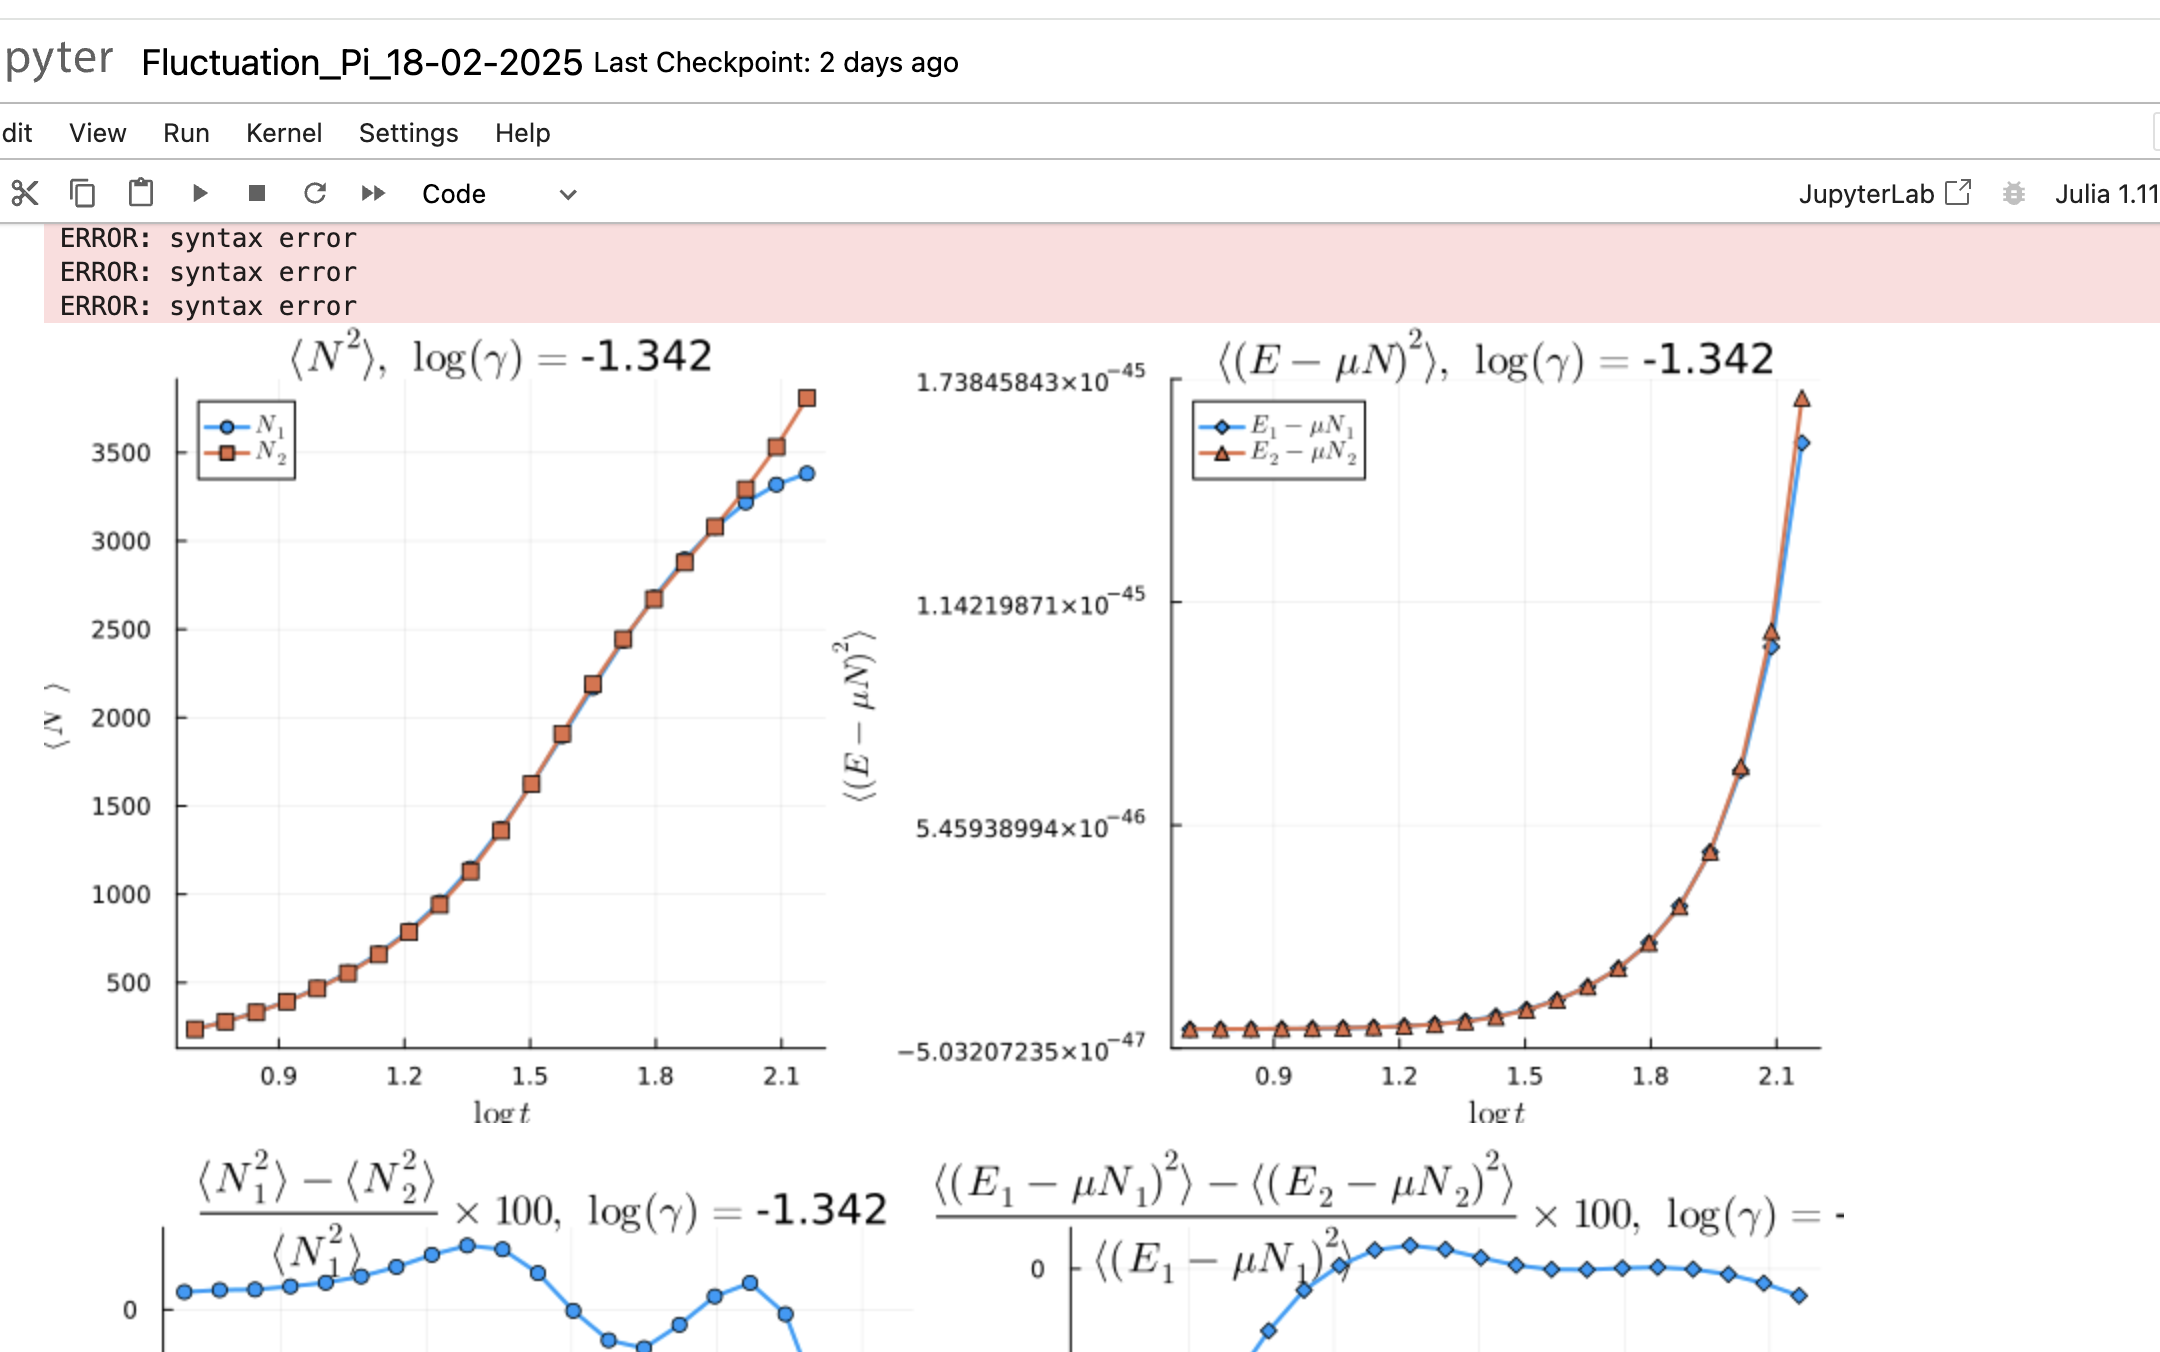
\includegraphics[width=1\textwidth]{Figures/test}

%\begin{aff}
%Donc une a l'ordre un en $\delta \theta (\operator{A}^{(0)})^{-1} %\operator{V}$ 

%\begin{eqnarray*}
%	\langle \delta \Pi ( \theta) \delta \Pi ( \theta') \rangle & = &  ( (\Pi^c_s - \Pi^c)\Pi^c/\Pi^c_s ) ( \theta ) \delta_{\theta, \theta'}/\delta \theta + \mathscr{F}(\theta , \theta' ) ,	
%\end{eqnarray*}

%avec 

%\begin{eqnarray*}
%	\mathscr{F}(\theta , \theta' ) & = & \left [ (\Pi^c_s - \Pi^c )( \theta)  +  (\Pi^c_s - \Pi^c ) ( \theta' )\right ] \frac{\Pi^c}{\Pi^c_s}(\theta)\frac{\Pi^c}{\Pi^c_s}(\theta') \frac{ \Delta( \theta'- \theta )}{ 2 \pi }\\
%	&&  - \left [ (\Pi^c_s - \Pi^c )( \theta)   (\Pi^c_s - \Pi^c ) ( \theta' )\right ] \frac{\Pi^c}{\Pi^c_s}(\theta)\frac{\Pi^c}{\Pi^c_s}(\theta')\int d\theta'' \left (   \frac{ \Pi^c/\Pi^c_s}{\Pi^c_s - \Pi^c} \right )(\theta'') \frac{\Delta(\theta''- \theta)}{2 \pi}\frac{\Delta(\theta''- \theta')}{2 \pi}  	
%\end{eqnarray*}
%\end{aff}



 








\subsection{Entropie de Yang-Yang généralisée}



\chapter{Dynamique hors-équilibre et hydrodynamique généralisée}
\minitoc
\section{Hydrodynamique et régimes asymptotiques}

\subsection{Hydrodynamique classique des systèmes chaotiques}
\subsection{Hydrodynamique des systèmes intégrables et distribution de rapidité}
\subsection{Équation d’hydrodynamique généralisée (GHD)}

\chapter{Fluctuation de la distribution de rapidité dans des état d'équilibre} 
%Dans ce chapitre, nous nous intéressons aux fluctuations de la distribution de rapidité \( \delta \rho \) autour d'une distribution de référence \( \rho^c \), qui maximise la contribution à la fonction de partition des états, exprimée comme une fonctionnelle de la distribution \( \rho \) : 

La fonction de partition des états, s'exprime comme une fonctionnelle de la distribution \( \rho \) : 

\begin{eqnarray*}
	\Xi & = & \sum_\rho \exp \left( -\mathcal{A}(\rho) \right).
\end{eqnarray*}  

Dans la section {\em \bf Entropie de Yang-Yang} (\ref{??}), l'action \( \mathcal{A}(\rho) \) s'écrit sous la forme :  

\begin{eqnarray*}
	\mathcal{A}(\rho) & \doteq & - L\mathcal{S}_{YY}(\rho) + L\int f(\theta) \rho (\theta) \, d\theta,		
\end{eqnarray*}  

où \( \mathcal{S}_{YY} \) est la fonctionnelle d'entropie de Yang-Yang, définie dans (\ref{??}), et \( f \) est la fonction paramétrant les charges, introduite dans (\ref{??}).  

Dans cette même section {\em \bf Entropie de Yang-Yang} (\ref{??}), nous avons établi un lien entre \( f \) et distribution de référence \( \rho^c \), qui maximise la contribution à la fonction de partition des états .\\

On veux tester si nos experience est décrit pas un GGE. Pour cela nous nous intéressons aux fluctuations de la distribution de rapidité \( \delta \rho \) autour \( \rho^c \).

%Nous poursuivons à présent avec cette définition de l'action de classe $\mathcal{C}^2$ et admetant une distribution critique $\rho^c$ tel que sa différentielle en ce point critique soit nulle $d\mathcal{A}_{\rho^c} = 0 $ (\ref{??}) de sorte que d'aprés la formule de Taylor-Youg %afin de déterminer les fluctuations autour de \( \Pi^c \). Pour cela, nous réécrivons l'action sous la forme :  

Nous poursuivons à présent avec cette définition de l'action de classe $\mathcal{C}^2$ et admetant une distribution critique $\rho^c$ tel que sa différentielle en ce point critique soit nulle $d\mathcal{A}_{\rho^c} = 0 $ (\ref{??}) de sorte que d'aprés la formule de Taylor-Youg %afin de déterminer les fluctuations autour de \( \Pi^c \). Pour cela, nous réécrivons l'action sous la forme :  

\begin{eqnarray*}  
	\mathcal{A}(\rho^c + \delta \rho) & \underset{ \delta \rho \to 0 }{=} & \mathcal{A}(\rho^c)  + \frac{1}{2} \left. \frac{\delta^2 \mathcal{A}}{\delta \rho^2} \right|_{\rho^c} (\delta \rho) + \mathcal{O}((\delta \rho)^3),  
\end{eqnarray*}  

une expression quadratique pour l'action à l'ordre dominant en \( \delta \Pi \) avec $\left. \frac{\delta^2 \mathcal{A}}{\delta \rho^2} \right|_{\rho^c}$ la forme quadratique définie positive (Fig (\ref{fig.fluctu.A})).

\begin{figure}[H]
	\centering 
	\begin{tikzpicture}
		\begin{scope}[shift={(0,0)}]
			\begin{scope}[transform canvas={scale=0.6}]
				% Définition des couleurs avec les codes HTML
\definecolor{colorOne}{HTML}{443E46}
\definecolor{colorTwo}{HTML}{F6DEB8}
\definecolor{colorThree}{HTML}{908CA4}
\definecolor{colorFour}{HTML}{57659E}
\definecolor{colorFive}{HTML}{C57284}
\definecolor{colorSix}{HTML}{FF5B69}

% Raccourcis pour les couleurs
\def\colorOne{colorOne}
\def\colorTwo{colorTwo}
\def\colorThree{colorThree}
\def\colorFour{colorFour}
\def\colorFive{colorFive}
\def\colorSix{colorSix}

\def\colorslide{blue!50!black}



\begin{scope}
	% Tracer une courbe lisse entre des points
	\draw[shift={(0,0)} ,\colorOne]
		(-1 , 0 ) edge [thick,line width=0.8ex , ->,>=triangle 45  , \colorOne] node [pos = 1 , below ]{\huge$\rho$}( 5  , 0 )
	;
	\draw[shift={(0,0)}, color=\colorOne]
		(0, -1.0 ) edge [thick,line width=0.8ex , ->,>=triangle 45  ]node [pos=0.9,left=0.2cm ]{\huge$\mathcal{A}(\rho)$}( 0  , 5 )
	;
	\draw[]
		(2.5, 0.12 ) edge [thick,line width=0.8ex ,\colorThree ]node [pos=1,below  ]{\huge$\rho^c$} (2.5, -0.12 )	
	;
	
	\draw[]
		(2.5, -0.12 ) edge [thick,line width=0.4ex , dashed, \colorThree ] (2.5, 5.5 )
		(1.5, 1 ) edge [thick,line width=0.4ex , <->,>=triangle 45  , \colorThree ] (3.5, 1 )
		(-0.3,1) edge [thick,line width=0.4ex  , \colorThree ] node [pos=0,left ]{\huge$\mathcal{A}(\rho^c)$} (0.3, 1 )	
	;
    \draw[thick, line width=0.8ex , \colorFour] plot[smooth, tension=0.7] coordinates {
        (1, 5) (1.6 , 3 ) (2.5, 1) (3.5 , 3 )  (4, 5)
    };		
	
\end{scope}

	
			
			\end{scope}
			
			\draw[color = red , scale = 0.5 , draw = none  ] (-2 , -1) rectangle (5, 6) ; 	
		\end{scope}
		
		\begin{scope}[shift={(19,-1)}]
			\begin{scope}[transform canvas={scale=0.6}]
				% Définition des couleurs avec les codes HTML
\definecolor{colorOne}{HTML}{443E46}
\definecolor{colorTwo}{HTML}{F6DEB8}
\definecolor{colorThree}{HTML}{908CA4}
\definecolor{colorFour}{HTML}{57659E}
\definecolor{colorFive}{HTML}{C57284}
\definecolor{colorSix}{HTML}{FF5B69}

% Raccourcis pour les couleurs
\def\colorOne{colorOne}
\def\colorTwo{colorTwo}
\def\colorThree{colorThree}
\def\colorFour{colorFour}
\def\colorFive{colorFive}
\def\colorSix{colorSix}

\def\colorslide{blue!50!black}

\def\Occupation{
	\def\traitx{0.3}
	\def\traity{0.5}
	\draw[shift={(0,0)}]
		(-13.5 , 0 ) edge [thick,line width=0.8ex ]( -3.2  , 0 )
		( -3.2 - \traitx  , 0 - \traity ) edge [thick,line width=0.8ex ]( -3.2 + \traitx  , 0 + \traity  )
		( -2.8 - \traitx  , 0 - \traity ) edge [thick,line width=0.8ex ]( -2.8 + \traitx  , 0 + \traity  )
		(-2.8 , 0 ) edge [thick,line width=0.8ex ](2.8  , 0 )
		( 2.8 - \traitx  , 0 - \traity ) edge [thick,line width=0.8ex ]( 2.8 + \traitx  , 0 + \traity  )
		( 3.2 - \traitx  , 0 - \traity ) edge [thick,line width=0.8ex ]( 3.2 + \traitx  , 0 + \traity  )
		(3.2, 0 ) edge [thick,line width=0.8ex,->,>=triangle 45 , color = black ]node [pos=1.01,below  ]{\huge$\theta$}	( 13  , 0 )
	;
	\draw[shift={(0,0)}, color=\colorOne]
		(-10.5 , -1.5 ) edge [thick,line width=0.8ex , ->,>=triangle 45  ]( -10.5  , 4.5 )
	;
		
	\foreach \r in {1 , ... , 3 } {
%		\draw[
%		decoration={
%		markings,
%    	mark connection node=my node,
%    	mark=at position 0 with{\node [blue,transform shape] (my node) {\large \r};}},
%		color=gray, thick, 
%		line width=0.5ex] decorate { 
%            (-11.0, \r) -- (-10.1, \r )}
%        ;
        \draw[
			color=\colorOne,
			] 
            (-11.0, \r) edge[color=\colorThree , thick,line width=0.5ex] node [pos=-0.5 ]{\large\color{\colorFour} $\frac{\r}{\delta \theta}$ } (-10.3, \r )
        	;
	
	}
	

	
	% Graduation abcsisse 
	% Définitions des listes
% Definitions of the lists
\def\listetuple{-9/\theta_{1}, -8/\theta_{2} , -5/\theta_{3} , -2/\theta_{a-1} , 0/\theta_{a} , 1/\theta_{a+1} , 2/\theta_{a+2} ,  5/\theta_{N-4} , 7/\theta_{N-3},8/\theta_{N-1},9/\theta_{N} }
\def\listetrais{-12 , -11, -10, -9 , -8 , -7 ,  -6 , -5, -4.5,-4, -2 , -1, 0 , 0.5, 1, 2, 4 , 5 ,  6 , 7 , 8 ,8.5, 9 ,  10 , 11, 12 }

% Loop over listetrais
\foreach \r in \listetrais {
    % Initialize found variable to zero
    % Initialize found variable to zero
    %\pgfmathsetmacro\found{0}
    \global\def\found{0}
    \xdef\nomtheta{}
    
    % Check if \r is in listetuple
    \foreach \x/\y in \listetuple { 
        \ifdim \r pt=\x pt % If \r matches any \x in listetuple
            \global\def\found{1} ;
            \xdef\nomtheta{\y} % Set \nomtheta to the corresponding \y
            %\pgfmathsetmacro\found{1} % Set found to 1            
            %\global\pgfmathsetmacro\found{1}
        \fi
    }
    
    %\node [circle, draw, red] (A) at (\r, 2) {\found , $\nomtheta$};
    
    % Draw the line and display \nomtheta if found
    \ifnum\found=1
        \draw[color=\colorOne, thick, line width=0.5ex] 
            (\r, -0.3) -- (\r, 0.3) node[red , pos=-0.5] {\large $\nomtheta$};
         \filldraw[line width=0.5ex, color=\colorSix, outer color=\colorSix, inner color=\colorSix] 
            (\r, 0) circle (4pt);
    \else 
        % Draw without \nomtheta and add a blue circle if not found
        \draw[color=\colorOne, thick, line width=0.5ex] 
            (\r, -0.3) -- (\r, 0.3);
        \filldraw[line width=0.5ex, color=\colorSix, outer color=\colorTwo, inner color=\colorTwo] 
            (\r, 0) circle (4pt); 
    \fi
}

\def\listetrais{-9.5/\theta_{i-1}/2/3, -6.5/\theta_{i}/1/4  ,   -1.5/\theta_{j}/2/4 , 1.5/\theta_{j+1}/-1/3 , 3.5/\theta_{\ell-1}/1/3 , 6.5/\theta_{\ell}/3/4 , 9.5/\theta(\theta_{\ell+1})/-1/3 };



\foreach \r/\nomx/\y/\ys in \listetrais {
	\draw[
		decoration={
		markings,
    	mark connection node=my node,
    	mark=at position .5 with{\node [blue,transform shape] (my node) {\large \color{\colorFour} $\nomx$};}},
		color=\colorThree , thick, 
		line width=0.5ex] decorate { 
            (\r, 0.12) -- (\r, -1.2)}
        ;
     
     \ifdim \y pt > -1 pt 
     	\draw[
			decoration={
			markings,
    		mark connection node=my node,
    		mark=at position .5 with{\node [blue,transform shape] (my node) {\large \color{\colorFour} $\Pi(\nomx) $};}},
			color=\colorThree, thick, 
			line width=0.5ex] decorate { 
            (\r, \y) -- (\r +3, \y)}
        ;
        \draw[
			decoration={
			markings,
    		mark connection node=my node,
    		mark=at position .5 with{\node [blue,transform shape] (my node) {\large \color{\colorFive} $\Pi_s(\nomx) $};}},
			color=\colorFive, thick, 
			line width=0.5ex] decorate { 
            (\r, \ys) -- (\r +3, \ys)}
        ;
     \fi 
     \ifdim \r pt= -1.5 pt
     	\draw[
     		decoration={
			markings,
    		mark connection node=my node,
    		mark=at position .5 with{\node [blue,transform shape] (my node) {\large \color{\colorFour}  $\delta \theta $};},
    		%mark=at position 0.1  with {\arrow[blue, line width=0.5ex]{<}},
    		%mark=at position 1  with {\arrow[blue, line width=0.5ex]{>}}
    		},
        	color=\colorThree,
        	thick,
        	line width=0.5ex,
        	%arrows={Computer Modern Rightarrow[line cap=round]-Computer Modern Rightarrow[line cap=round]}
   			](\r, -1.2) edge[arrows={Computer Modern Rightarrow[line cap=round]-}] (\r + 0.4, -1.2)decorate {
    		(\r, -1.2) -- (\r + 3, -1.2)}(\r + 2, -1.2) edge[arrows={-Computer Modern Rightarrow[line cap=round]}] (\r + 3, -1.2)
    		;
    \fi
			
	
}


			
}


\begin{scope}
	%\draw[help lines , width=1.5ex] (-8,-3) grid (8,3);\draw[help lines ,width=0.5ex , opacity = 0.5] (-3,-3) grid[step=0.1] (3,3));
	
	%\draw[help lines] 
	%	(-3,-3) edge[width=1.5ex] grid (3,3)	
	%	(-3,-3) edge[width=0.5ex , opacity = 0.5] grid (3,3)	
	%;
	\begin{scope}[shift={(0,1)},rotate=0,opacity=1,color=black]
		\Occupation	
		
		%\node[anchor=east, font=\bfseries] at (-11, 0) {\color{red}\large (T = 0 )} ;	
	\end{scope}
	
	
	
	
	\begin{scope}[shift={(-10.5,7)},rotate=0,opacity=1,color=black]
	
	\begin{scope}[shift={(-0,0)},rotate=0,opacity=1,color=black]
	
		\draw[shift={(0,0)} ,line width=1ex,rounded corners = 1ex,color=\colorOne , opacity =1 ,fill=\colorOne!00 , pattern={north east lines} , pattern color=\colorOne!00 ]
			(0 , -1 ) rectangle (5,1)
		;
		

		\begin{scope}[shift={(0.5,0.5)}]
			\draw[color=\colorOne, thick, line width=0.5ex] 
            (0, -0.3) -- (0, 0.3) ;
            \filldraw[line width=0.5ex, color=\colorSix, outer color=\colorSix, inner color=\colorSix] 
            (0, 0) circle (4pt);
            
            \node[anchor=west, font=\bfseries] at (0.2, 0) {\color{\colorSix}\large : quasi-particule};
		\end{scope}
		
		\begin{scope}[shift={(0.5,-0.5)}]
			\draw[color=\colorOne, thick, line width=0.5ex] 
            (0, -0.3) -- (0, 0.3) ;
            \filldraw[line width=0.5ex, color=\colorSix, outer color=\colorTwo, inner color=\colorTwo] 
            (0, 0) circle (4pt);
            
            \node[anchor=west, font=\bfseries] at (0.2, 0) {\color{\colorSix}\large : hole};
		\end{scope}

	\end{scope}
	
	\begin{scope}[shift={(6,0)},rotate=0,opacity=1,color=black]	
		
		\draw[shift={(0,0)} ,line width=1ex,rounded corners = 1ex,color=\colorOne , opacity =1 ,fill=\colorOne!00 , pattern={north east lines} , pattern color=\colorOne!00 ]
			(0 , -1 ) rectangle (7.5,1)
		;
		
		\node[anchor=west] at (0.5, 0.5) {\color{\colorFour}\large $\Pi$ };\node[anchor=west, font=\bfseries] at (1, 0.5) {\color{\colorFour}\large : quasi-particule distribution};
		
		\node[anchor=west] at (0.5, -0.5) {\color{\colorFour}\large $\Pi_h$ };\node[anchor=west, font=\bfseries] at (1, -0.5) {\color{\colorFour}\large  : hole distribution};
		
	\end{scope}
	
	\begin{scope}[shift={(14.5,0)},rotate=0,opacity=1,color=black]	
		
		\draw[shift={(0,0)} ,line width=1ex,rounded corners = 1ex,color=\colorOne , opacity =1 ,fill=\colorOne!00 , pattern={north east lines} , pattern color=\colorOne!00 ]
			(0 , -0.5 ) rectangle (7.0,0.5)
		;
		
		\node[anchor=west] at (0.2, 0) {\color{\colorFour}\large ${\color{\colorFive}\Pi_s} = \Pi + \Pi_h $ } node[anchor=west , font=\bfseries] at (3.1 , 0 )  {\color{\colorFour}\large {\color{\colorFive} : density of states}};
		
	\end{scope}
	
	
	\end{scope}


		
	
\end{scope}

	
			
			\end{scope}
			\begin{scope}[scale=1]
				\draw[color = red , scale = 1 , draw = none  ] (-1 , -1) rectangle (5, 5) ; 
			\end{scope}	
		\end{scope}

		
				
			
	\end{tikzpicture}	
	\captionsetup{skip=10pt} % Ajoute de l’espace après la légende
	\label{fig.fluctu.A}
\end{figure}


On discrétise l'axe des rapidités en  petite cellule de rapidité $[\theta, \theta+\delta\theta]$, qui contient $L\rho(\theta) \delta \theta$ rapidités. 
	



Avec ces petites tranches, la forme quadratique s’écrit :

\begin{eqnarray*}
    \left. \frac{\delta^2 \mathcal{A}}{{\delta \rho}^2} \right|_{\rho^c}(\delta \rho ) &=&  \sum_{a,b \mid \text{tranche}}  
    \delta \rho(\theta_a)  \frac{\partial^2 \mathcal{A}}{\partial \delta \rho(\theta_a) \partial \delta \rho(\theta_b) } (\rho^c)  \delta \rho(\theta_b).
\end{eqnarray*}
Les fluctuations s’écrivent donc :

\begin{eqnarray*}
    \langle \delta \rho ( \theta) \delta \rho ( \theta') \rangle &=&  
    \frac{ \int d\delta \rho \, \delta \rho(\theta) \delta \rho ( \theta') 
    \exp \left( - \frac{1}{2} \sum_{a,b \mid \text{tranche}}  
    \delta \rho(\theta_a) \frac{\partial^2 \mathcal{A}}{\partial \delta \rho(\theta_a) \partial \delta \rho(\theta_b) } (\rho^c)  \delta \rho(\theta_b) \right) }
    { \int d\delta \Pi  
    \exp \left( - \frac{1}{2} \sum_{a,b \mid \text{tranche}}  
    \delta \rho(\theta_a) \frac{\partial^2 \mathcal{A}}{\partial \delta \rho(\theta_a) \partial \delta \rho(\theta_b) } (\rho^c)  \delta \rho(\theta_b) \right) } \\
    &=& \left( \mathbf{A}^{-1} \right)_{\theta , \theta'}
\end{eqnarray*}


\begin{aff}

\begin{eqnarray*}
	\langle \delta \rho ( \theta) \delta \rho ( \theta') \rangle &=& 	\left( \mathbf{A}^{-1} \right)_{\theta , \theta'}
\end{eqnarray*}

	
avec la  {\em matrice hessienne} $\mathbf{A}_{\theta , \theta'} \equiv \frac{\partial^2 \mathcal{A}}{\partial \delta \rho(\theta) \partial \delta \rho(\theta') }(\rho^c)$, au point critique/ qui maximise la probabilité  $\rho^c=\rho^c_s \nu^c $, s'écrit

\begin{eqnarray*}
	\operator{A} & = & \operator{A}^{(0)} + \delta \theta \operator{V}
\end{eqnarray*}

avec 

\begin{eqnarray*}
	A^{(0)}_{\theta , \theta'}  & = &  L\delta \theta \left ( \frac{ 1}{\rho^c_s ( 1  - \nu^c ) \nu^c } \right )(\theta)    \delta({\theta - \theta '})	,\\
	V_{\theta , \theta'}  &= & L \delta \theta \left \{ - \left [ \left ( \frac{1}{\rho^c_s( 1 - \nu^c) } \right ) ( \theta)  +  \left ( \frac{1}{\rho^c_s( 1 - \nu^c) } \right ) ( \theta' )\right ] \frac{ \Delta( \theta'- \theta )}{ 2 \pi } + \int d\theta''  \left ( \frac{\nu^c}{\rho^c_s( 1 - \nu^c) } \right )(\theta'') \frac{\Delta(\theta''- \theta)}{2 \pi}\frac{\Delta(\theta''- \theta')}{2 \pi}   \right \} 	
\end{eqnarray*}

\end{aff}

\subsection{Testes}

\begin{eqnarray*}
	\Delta_{\operator{\mathcal{N}}}^2  & = &  \frac{1}{\beta} \left . \frac{\partial \langle \operator{\mathcal{N}} \rangle}{\partial \mu} \right )_T \\
	\Delta_{\operator{\mathcal{E}}-\mu \operator{\mathcal{N}}}^2  & = &  - \left . \frac{\partial \langle \operator{\mathcal{E}}-\mu \operator{\mathcal{N}} \rangle}{\partial \beta} \right )_\mu 
\end{eqnarray*}

et 

\begin{eqnarray*}
	\Delta_{\operator{\mathcal{N}}}^2  &= & L^2 \int d\theta_a \int d \theta_b \, \langle \delta \rho(\theta_a) \delta \rho(\theta_b) \rangle \\
	\Delta_{\operator{\mathcal{E}}-\mu \operator{\mathcal{N}}}^2  & = & L^2 \int d\theta_a \int d \theta_b \, \left ( - \mu + \frac{1}2 m \theta_a^2  \right  )\left ( - \mu + \frac{1}2 m \theta_b^2  \right  )  \langle \delta \rho(\theta_a) \delta \rho(\theta_b) \rangle
\end{eqnarray*}

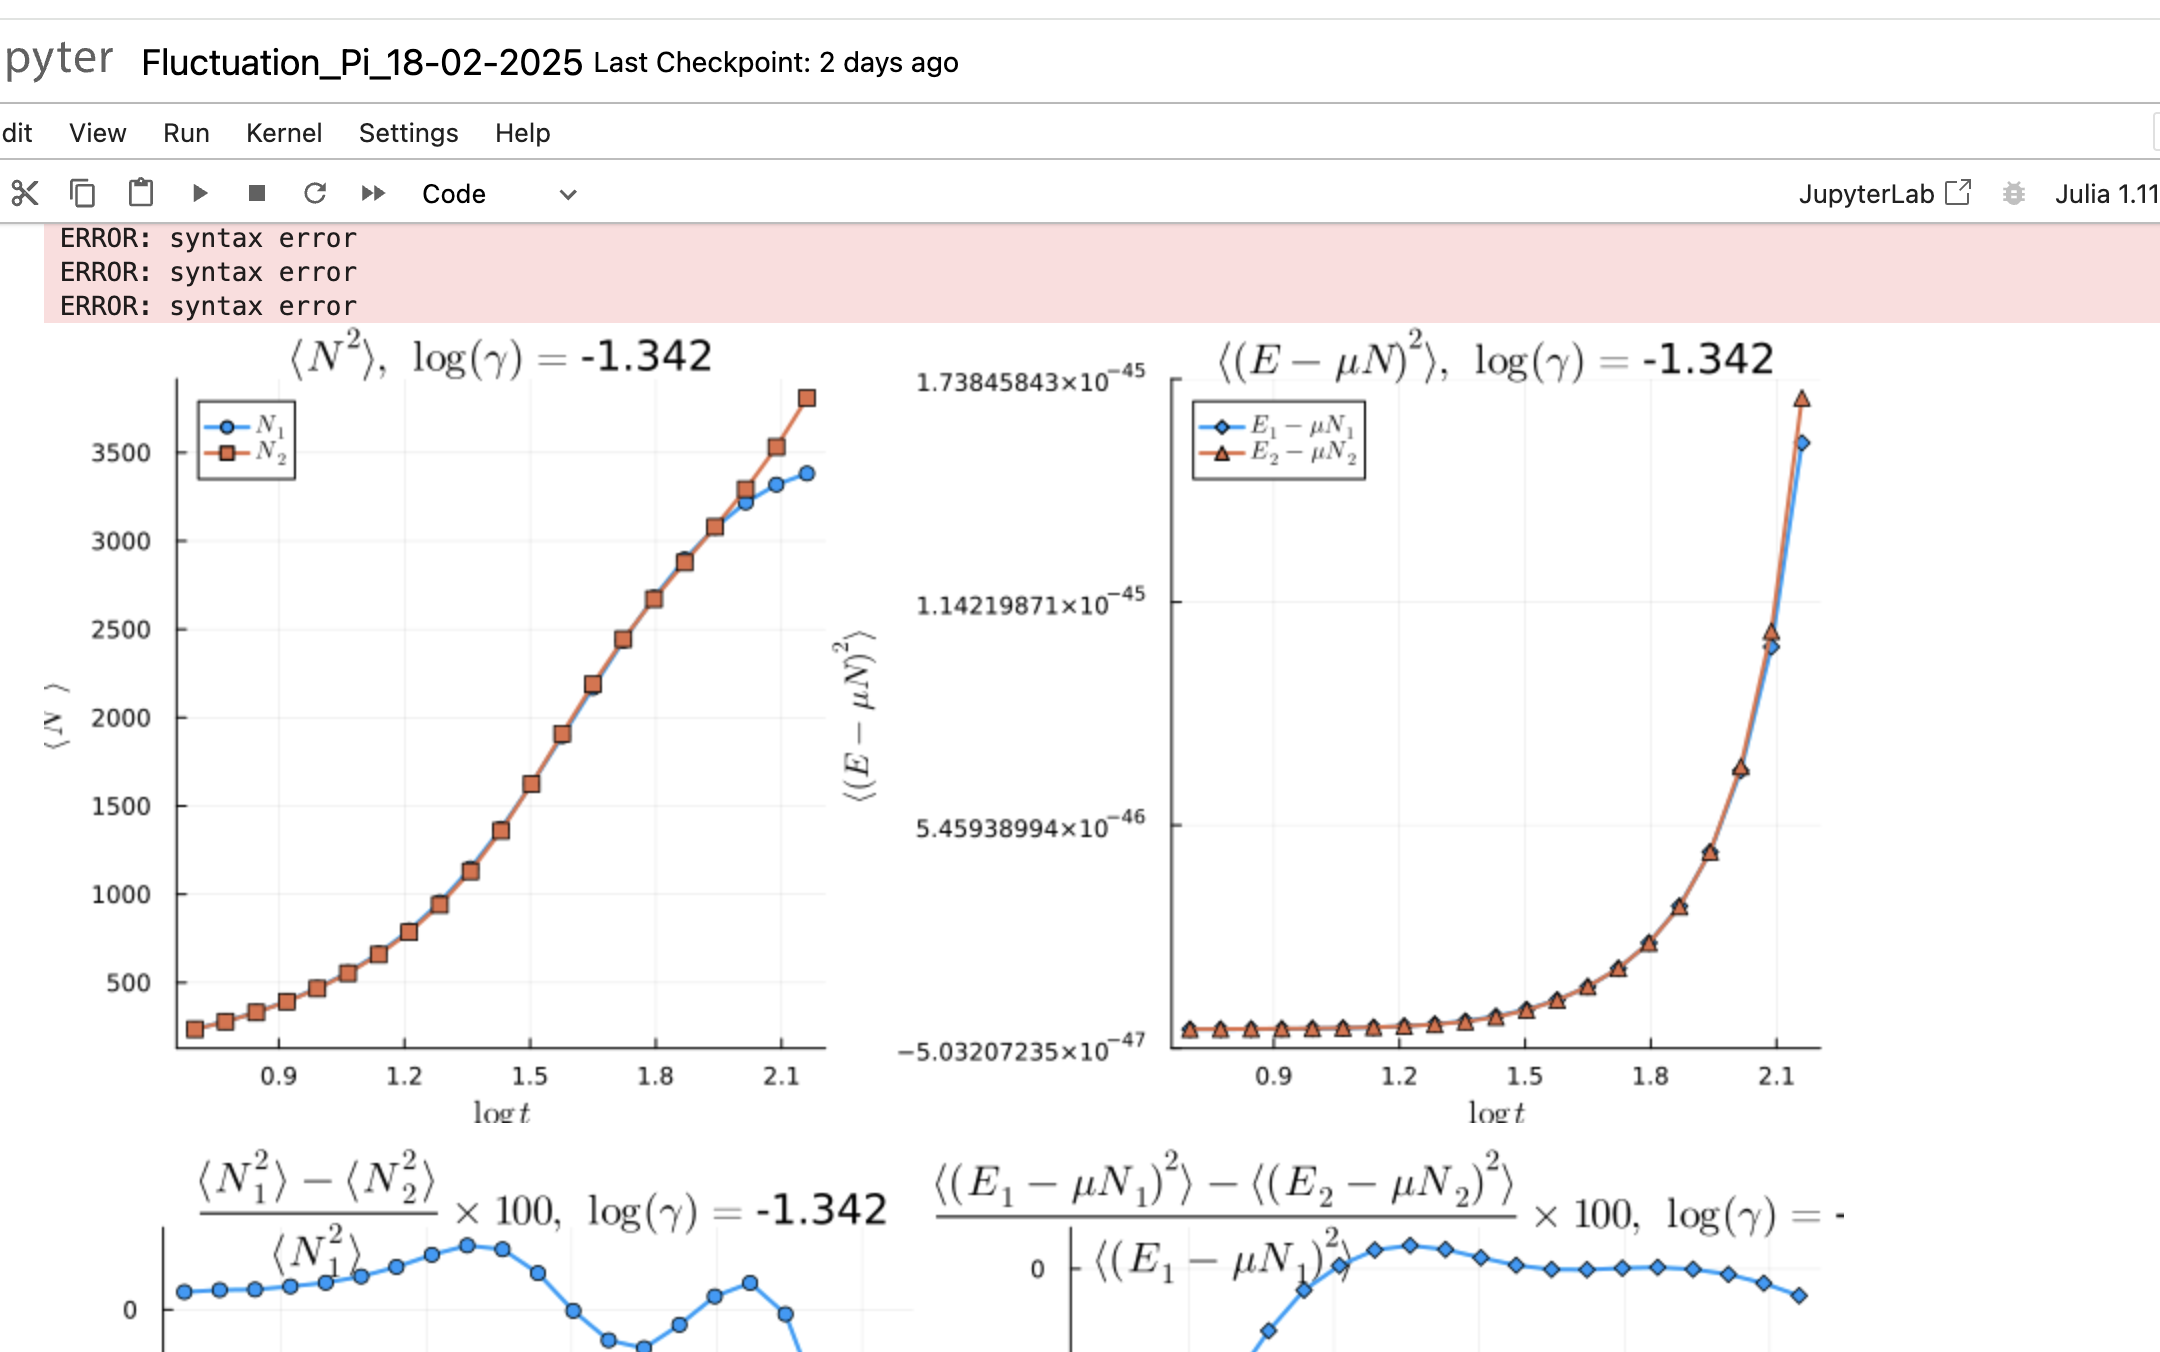
\includegraphics[width=1\textwidth]{Figures/test}

%\begin{aff}
%Donc une a l'ordre un en $\delta \theta (\operator{A}^{(0)})^{-1} %\operator{V}$ 

%\begin{eqnarray*}
%	\langle \delta \Pi ( \theta) \delta \Pi ( \theta') \rangle & = &  ( (\Pi^c_s - \Pi^c)\Pi^c/\Pi^c_s ) ( \theta ) \delta_{\theta, \theta'}/\delta \theta + \mathscr{F}(\theta , \theta' ) ,	
%\end{eqnarray*}

%avec 

%\begin{eqnarray*}
%	\mathscr{F}(\theta , \theta' ) & = & \left [ (\Pi^c_s - \Pi^c )( \theta)  +  (\Pi^c_s - \Pi^c ) ( \theta' )\right ] \frac{\Pi^c}{\Pi^c_s}(\theta)\frac{\Pi^c}{\Pi^c_s}(\theta') \frac{ \Delta( \theta'- \theta )}{ 2 \pi }\\
%	&&  - \left [ (\Pi^c_s - \Pi^c )( \theta)   (\Pi^c_s - \Pi^c ) ( \theta' )\right ] \frac{\Pi^c}{\Pi^c_s}(\theta)\frac{\Pi^c}{\Pi^c_s}(\theta')\int d\theta'' \left (   \frac{ \Pi^c/\Pi^c_s}{\Pi^c_s - \Pi^c} \right )(\theta'') \frac{\Delta(\theta''- \theta)}{2 \pi}\frac{\Delta(\theta''- \theta')}{2 \pi}  	
%\end{eqnarray*}
%\end{aff}



 









%%\chapter{Fluctuations et corrections à l’hydrodynamique généralisée}
%%\minitoc
%%\section{Fluctuations de la distribution de rapidité}
%%%Dans ce chapitre, nous nous intéressons aux fluctuations de la distribution de rapidité \( \delta \rho \) autour d'une distribution de référence \( \rho^c \), qui maximise la contribution à la fonction de partition des états, exprimée comme une fonctionnelle de la distribution \( \rho \) : 

La fonction de partition des états, s'exprime comme une fonctionnelle de la distribution \( \rho \) : 

\begin{eqnarray*}
	\Xi & = & \sum_\rho \exp \left( -\mathcal{A}(\rho) \right).
\end{eqnarray*}  

Dans la section {\em \bf Entropie de Yang-Yang} (\ref{??}), l'action \( \mathcal{A}(\rho) \) s'écrit sous la forme :  

\begin{eqnarray*}
	\mathcal{A}(\rho) & \doteq & - L\mathcal{S}_{YY}(\rho) + L\int f(\theta) \rho (\theta) \, d\theta,		
\end{eqnarray*}  

où \( \mathcal{S}_{YY} \) est la fonctionnelle d'entropie de Yang-Yang, définie dans (\ref{??}), et \( f \) est la fonction paramétrant les charges, introduite dans (\ref{??}).  

Dans cette même section {\em \bf Entropie de Yang-Yang} (\ref{??}), nous avons établi un lien entre \( f \) et distribution de référence \( \rho^c \), qui maximise la contribution à la fonction de partition des états .\\

On veux tester si nos experience est décrit pas un GGE. Pour cela nous nous intéressons aux fluctuations de la distribution de rapidité \( \delta \rho \) autour \( \rho^c \).

%Nous poursuivons à présent avec cette définition de l'action de classe $\mathcal{C}^2$ et admetant une distribution critique $\rho^c$ tel que sa différentielle en ce point critique soit nulle $d\mathcal{A}_{\rho^c} = 0 $ (\ref{??}) de sorte que d'aprés la formule de Taylor-Youg %afin de déterminer les fluctuations autour de \( \Pi^c \). Pour cela, nous réécrivons l'action sous la forme :  

Nous poursuivons à présent avec cette définition de l'action de classe $\mathcal{C}^2$ et admetant une distribution critique $\rho^c$ tel que sa différentielle en ce point critique soit nulle $d\mathcal{A}_{\rho^c} = 0 $ (\ref{??}) de sorte que d'aprés la formule de Taylor-Youg %afin de déterminer les fluctuations autour de \( \Pi^c \). Pour cela, nous réécrivons l'action sous la forme :  

\begin{eqnarray*}  
	\mathcal{A}(\rho^c + \delta \rho) & \underset{ \delta \rho \to 0 }{=} & \mathcal{A}(\rho^c)  + \frac{1}{2} \left. \frac{\delta^2 \mathcal{A}}{\delta \rho^2} \right|_{\rho^c} (\delta \rho) + \mathcal{O}((\delta \rho)^3),  
\end{eqnarray*}  

une expression quadratique pour l'action à l'ordre dominant en \( \delta \Pi \) avec $\left. \frac{\delta^2 \mathcal{A}}{\delta \rho^2} \right|_{\rho^c}$ la forme quadratique définie positive (Fig (\ref{fig.fluctu.A})).

\begin{figure}[H]
	\centering 
	\begin{tikzpicture}
		\begin{scope}[shift={(0,0)}]
			\begin{scope}[transform canvas={scale=0.6}]
				% Définition des couleurs avec les codes HTML
\definecolor{colorOne}{HTML}{443E46}
\definecolor{colorTwo}{HTML}{F6DEB8}
\definecolor{colorThree}{HTML}{908CA4}
\definecolor{colorFour}{HTML}{57659E}
\definecolor{colorFive}{HTML}{C57284}
\definecolor{colorSix}{HTML}{FF5B69}

% Raccourcis pour les couleurs
\def\colorOne{colorOne}
\def\colorTwo{colorTwo}
\def\colorThree{colorThree}
\def\colorFour{colorFour}
\def\colorFive{colorFive}
\def\colorSix{colorSix}

\def\colorslide{blue!50!black}



\begin{scope}
	% Tracer une courbe lisse entre des points
	\draw[shift={(0,0)} ,\colorOne]
		(-1 , 0 ) edge [thick,line width=0.8ex , ->,>=triangle 45  , \colorOne] node [pos = 1 , below ]{\huge$\rho$}( 5  , 0 )
	;
	\draw[shift={(0,0)}, color=\colorOne]
		(0, -1.0 ) edge [thick,line width=0.8ex , ->,>=triangle 45  ]node [pos=0.9,left=0.2cm ]{\huge$\mathcal{A}(\rho)$}( 0  , 5 )
	;
	\draw[]
		(2.5, 0.12 ) edge [thick,line width=0.8ex ,\colorThree ]node [pos=1,below  ]{\huge$\rho^c$} (2.5, -0.12 )	
	;
	
	\draw[]
		(2.5, -0.12 ) edge [thick,line width=0.4ex , dashed, \colorThree ] (2.5, 5.5 )
		(1.5, 1 ) edge [thick,line width=0.4ex , <->,>=triangle 45  , \colorThree ] (3.5, 1 )
		(-0.3,1) edge [thick,line width=0.4ex  , \colorThree ] node [pos=0,left ]{\huge$\mathcal{A}(\rho^c)$} (0.3, 1 )	
	;
    \draw[thick, line width=0.8ex , \colorFour] plot[smooth, tension=0.7] coordinates {
        (1, 5) (1.6 , 3 ) (2.5, 1) (3.5 , 3 )  (4, 5)
    };		
	
\end{scope}

	
			
			\end{scope}
			
			\draw[color = red , scale = 0.5 , draw = none  ] (-2 , -1) rectangle (5, 6) ; 	
		\end{scope}
		
		\begin{scope}[shift={(19,-1)}]
			\begin{scope}[transform canvas={scale=0.6}]
				% Définition des couleurs avec les codes HTML
\definecolor{colorOne}{HTML}{443E46}
\definecolor{colorTwo}{HTML}{F6DEB8}
\definecolor{colorThree}{HTML}{908CA4}
\definecolor{colorFour}{HTML}{57659E}
\definecolor{colorFive}{HTML}{C57284}
\definecolor{colorSix}{HTML}{FF5B69}

% Raccourcis pour les couleurs
\def\colorOne{colorOne}
\def\colorTwo{colorTwo}
\def\colorThree{colorThree}
\def\colorFour{colorFour}
\def\colorFive{colorFive}
\def\colorSix{colorSix}

\def\colorslide{blue!50!black}

\def\Occupation{
	\def\traitx{0.3}
	\def\traity{0.5}
	\draw[shift={(0,0)}]
		(-13.5 , 0 ) edge [thick,line width=0.8ex ]( -3.2  , 0 )
		( -3.2 - \traitx  , 0 - \traity ) edge [thick,line width=0.8ex ]( -3.2 + \traitx  , 0 + \traity  )
		( -2.8 - \traitx  , 0 - \traity ) edge [thick,line width=0.8ex ]( -2.8 + \traitx  , 0 + \traity  )
		(-2.8 , 0 ) edge [thick,line width=0.8ex ](2.8  , 0 )
		( 2.8 - \traitx  , 0 - \traity ) edge [thick,line width=0.8ex ]( 2.8 + \traitx  , 0 + \traity  )
		( 3.2 - \traitx  , 0 - \traity ) edge [thick,line width=0.8ex ]( 3.2 + \traitx  , 0 + \traity  )
		(3.2, 0 ) edge [thick,line width=0.8ex,->,>=triangle 45 , color = black ]node [pos=1.01,below  ]{\huge$\theta$}	( 13  , 0 )
	;
	\draw[shift={(0,0)}, color=\colorOne]
		(-10.5 , -1.5 ) edge [thick,line width=0.8ex , ->,>=triangle 45  ]( -10.5  , 4.5 )
	;
		
	\foreach \r in {1 , ... , 3 } {
%		\draw[
%		decoration={
%		markings,
%    	mark connection node=my node,
%    	mark=at position 0 with{\node [blue,transform shape] (my node) {\large \r};}},
%		color=gray, thick, 
%		line width=0.5ex] decorate { 
%            (-11.0, \r) -- (-10.1, \r )}
%        ;
        \draw[
			color=\colorOne,
			] 
            (-11.0, \r) edge[color=\colorThree , thick,line width=0.5ex] node [pos=-0.5 ]{\large\color{\colorFour} $\frac{\r}{\delta \theta}$ } (-10.3, \r )
        	;
	
	}
	

	
	% Graduation abcsisse 
	% Définitions des listes
% Definitions of the lists
\def\listetuple{-9/\theta_{1}, -8/\theta_{2} , -5/\theta_{3} , -2/\theta_{a-1} , 0/\theta_{a} , 1/\theta_{a+1} , 2/\theta_{a+2} ,  5/\theta_{N-4} , 7/\theta_{N-3},8/\theta_{N-1},9/\theta_{N} }
\def\listetrais{-12 , -11, -10, -9 , -8 , -7 ,  -6 , -5, -4.5,-4, -2 , -1, 0 , 0.5, 1, 2, 4 , 5 ,  6 , 7 , 8 ,8.5, 9 ,  10 , 11, 12 }

% Loop over listetrais
\foreach \r in \listetrais {
    % Initialize found variable to zero
    % Initialize found variable to zero
    %\pgfmathsetmacro\found{0}
    \global\def\found{0}
    \xdef\nomtheta{}
    
    % Check if \r is in listetuple
    \foreach \x/\y in \listetuple { 
        \ifdim \r pt=\x pt % If \r matches any \x in listetuple
            \global\def\found{1} ;
            \xdef\nomtheta{\y} % Set \nomtheta to the corresponding \y
            %\pgfmathsetmacro\found{1} % Set found to 1            
            %\global\pgfmathsetmacro\found{1}
        \fi
    }
    
    %\node [circle, draw, red] (A) at (\r, 2) {\found , $\nomtheta$};
    
    % Draw the line and display \nomtheta if found
    \ifnum\found=1
        \draw[color=\colorOne, thick, line width=0.5ex] 
            (\r, -0.3) -- (\r, 0.3) node[red , pos=-0.5] {\large $\nomtheta$};
         \filldraw[line width=0.5ex, color=\colorSix, outer color=\colorSix, inner color=\colorSix] 
            (\r, 0) circle (4pt);
    \else 
        % Draw without \nomtheta and add a blue circle if not found
        \draw[color=\colorOne, thick, line width=0.5ex] 
            (\r, -0.3) -- (\r, 0.3);
        \filldraw[line width=0.5ex, color=\colorSix, outer color=\colorTwo, inner color=\colorTwo] 
            (\r, 0) circle (4pt); 
    \fi
}

\def\listetrais{-9.5/\theta_{i-1}/2/3, -6.5/\theta_{i}/1/4  ,   -1.5/\theta_{j}/2/4 , 1.5/\theta_{j+1}/-1/3 , 3.5/\theta_{\ell-1}/1/3 , 6.5/\theta_{\ell}/3/4 , 9.5/\theta(\theta_{\ell+1})/-1/3 };



\foreach \r/\nomx/\y/\ys in \listetrais {
	\draw[
		decoration={
		markings,
    	mark connection node=my node,
    	mark=at position .5 with{\node [blue,transform shape] (my node) {\large \color{\colorFour} $\nomx$};}},
		color=\colorThree , thick, 
		line width=0.5ex] decorate { 
            (\r, 0.12) -- (\r, -1.2)}
        ;
     
     \ifdim \y pt > -1 pt 
     	\draw[
			decoration={
			markings,
    		mark connection node=my node,
    		mark=at position .5 with{\node [blue,transform shape] (my node) {\large \color{\colorFour} $\Pi(\nomx) $};}},
			color=\colorThree, thick, 
			line width=0.5ex] decorate { 
            (\r, \y) -- (\r +3, \y)}
        ;
        \draw[
			decoration={
			markings,
    		mark connection node=my node,
    		mark=at position .5 with{\node [blue,transform shape] (my node) {\large \color{\colorFive} $\Pi_s(\nomx) $};}},
			color=\colorFive, thick, 
			line width=0.5ex] decorate { 
            (\r, \ys) -- (\r +3, \ys)}
        ;
     \fi 
     \ifdim \r pt= -1.5 pt
     	\draw[
     		decoration={
			markings,
    		mark connection node=my node,
    		mark=at position .5 with{\node [blue,transform shape] (my node) {\large \color{\colorFour}  $\delta \theta $};},
    		%mark=at position 0.1  with {\arrow[blue, line width=0.5ex]{<}},
    		%mark=at position 1  with {\arrow[blue, line width=0.5ex]{>}}
    		},
        	color=\colorThree,
        	thick,
        	line width=0.5ex,
        	%arrows={Computer Modern Rightarrow[line cap=round]-Computer Modern Rightarrow[line cap=round]}
   			](\r, -1.2) edge[arrows={Computer Modern Rightarrow[line cap=round]-}] (\r + 0.4, -1.2)decorate {
    		(\r, -1.2) -- (\r + 3, -1.2)}(\r + 2, -1.2) edge[arrows={-Computer Modern Rightarrow[line cap=round]}] (\r + 3, -1.2)
    		;
    \fi
			
	
}


			
}


\begin{scope}
	%\draw[help lines , width=1.5ex] (-8,-3) grid (8,3);\draw[help lines ,width=0.5ex , opacity = 0.5] (-3,-3) grid[step=0.1] (3,3));
	
	%\draw[help lines] 
	%	(-3,-3) edge[width=1.5ex] grid (3,3)	
	%	(-3,-3) edge[width=0.5ex , opacity = 0.5] grid (3,3)	
	%;
	\begin{scope}[shift={(0,1)},rotate=0,opacity=1,color=black]
		\Occupation	
		
		%\node[anchor=east, font=\bfseries] at (-11, 0) {\color{red}\large (T = 0 )} ;	
	\end{scope}
	
	
	
	
	\begin{scope}[shift={(-10.5,7)},rotate=0,opacity=1,color=black]
	
	\begin{scope}[shift={(-0,0)},rotate=0,opacity=1,color=black]
	
		\draw[shift={(0,0)} ,line width=1ex,rounded corners = 1ex,color=\colorOne , opacity =1 ,fill=\colorOne!00 , pattern={north east lines} , pattern color=\colorOne!00 ]
			(0 , -1 ) rectangle (5,1)
		;
		

		\begin{scope}[shift={(0.5,0.5)}]
			\draw[color=\colorOne, thick, line width=0.5ex] 
            (0, -0.3) -- (0, 0.3) ;
            \filldraw[line width=0.5ex, color=\colorSix, outer color=\colorSix, inner color=\colorSix] 
            (0, 0) circle (4pt);
            
            \node[anchor=west, font=\bfseries] at (0.2, 0) {\color{\colorSix}\large : quasi-particule};
		\end{scope}
		
		\begin{scope}[shift={(0.5,-0.5)}]
			\draw[color=\colorOne, thick, line width=0.5ex] 
            (0, -0.3) -- (0, 0.3) ;
            \filldraw[line width=0.5ex, color=\colorSix, outer color=\colorTwo, inner color=\colorTwo] 
            (0, 0) circle (4pt);
            
            \node[anchor=west, font=\bfseries] at (0.2, 0) {\color{\colorSix}\large : hole};
		\end{scope}

	\end{scope}
	
	\begin{scope}[shift={(6,0)},rotate=0,opacity=1,color=black]	
		
		\draw[shift={(0,0)} ,line width=1ex,rounded corners = 1ex,color=\colorOne , opacity =1 ,fill=\colorOne!00 , pattern={north east lines} , pattern color=\colorOne!00 ]
			(0 , -1 ) rectangle (7.5,1)
		;
		
		\node[anchor=west] at (0.5, 0.5) {\color{\colorFour}\large $\Pi$ };\node[anchor=west, font=\bfseries] at (1, 0.5) {\color{\colorFour}\large : quasi-particule distribution};
		
		\node[anchor=west] at (0.5, -0.5) {\color{\colorFour}\large $\Pi_h$ };\node[anchor=west, font=\bfseries] at (1, -0.5) {\color{\colorFour}\large  : hole distribution};
		
	\end{scope}
	
	\begin{scope}[shift={(14.5,0)},rotate=0,opacity=1,color=black]	
		
		\draw[shift={(0,0)} ,line width=1ex,rounded corners = 1ex,color=\colorOne , opacity =1 ,fill=\colorOne!00 , pattern={north east lines} , pattern color=\colorOne!00 ]
			(0 , -0.5 ) rectangle (7.0,0.5)
		;
		
		\node[anchor=west] at (0.2, 0) {\color{\colorFour}\large ${\color{\colorFive}\Pi_s} = \Pi + \Pi_h $ } node[anchor=west , font=\bfseries] at (3.1 , 0 )  {\color{\colorFour}\large {\color{\colorFive} : density of states}};
		
	\end{scope}
	
	
	\end{scope}


		
	
\end{scope}

	
			
			\end{scope}
			\begin{scope}[scale=1]
				\draw[color = red , scale = 1 , draw = none  ] (-1 , -1) rectangle (5, 5) ; 
			\end{scope}	
		\end{scope}

		
				
			
	\end{tikzpicture}	
	\captionsetup{skip=10pt} % Ajoute de l’espace après la légende
	\label{fig.fluctu.A}
\end{figure}


On discrétise l'axe des rapidités en  petite cellule de rapidité $[\theta, \theta+\delta\theta]$, qui contient $L\rho(\theta) \delta \theta$ rapidités. 
	



Avec ces petites tranches, la forme quadratique s’écrit :

\begin{eqnarray*}
    \left. \frac{\delta^2 \mathcal{A}}{{\delta \rho}^2} \right|_{\rho^c}(\delta \rho ) &=&  \sum_{a,b \mid \text{tranche}}  
    \delta \rho(\theta_a)  \frac{\partial^2 \mathcal{A}}{\partial \delta \rho(\theta_a) \partial \delta \rho(\theta_b) } (\rho^c)  \delta \rho(\theta_b).
\end{eqnarray*}
Les fluctuations s’écrivent donc :

\begin{eqnarray*}
    \langle \delta \rho ( \theta) \delta \rho ( \theta') \rangle &=&  
    \frac{ \int d\delta \rho \, \delta \rho(\theta) \delta \rho ( \theta') 
    \exp \left( - \frac{1}{2} \sum_{a,b \mid \text{tranche}}  
    \delta \rho(\theta_a) \frac{\partial^2 \mathcal{A}}{\partial \delta \rho(\theta_a) \partial \delta \rho(\theta_b) } (\rho^c)  \delta \rho(\theta_b) \right) }
    { \int d\delta \Pi  
    \exp \left( - \frac{1}{2} \sum_{a,b \mid \text{tranche}}  
    \delta \rho(\theta_a) \frac{\partial^2 \mathcal{A}}{\partial \delta \rho(\theta_a) \partial \delta \rho(\theta_b) } (\rho^c)  \delta \rho(\theta_b) \right) } \\
    &=& \left( \mathbf{A}^{-1} \right)_{\theta , \theta'}
\end{eqnarray*}


\begin{aff}

\begin{eqnarray*}
	\langle \delta \rho ( \theta) \delta \rho ( \theta') \rangle &=& 	\left( \mathbf{A}^{-1} \right)_{\theta , \theta'}
\end{eqnarray*}

	
avec la  {\em matrice hessienne} $\mathbf{A}_{\theta , \theta'} \equiv \frac{\partial^2 \mathcal{A}}{\partial \delta \rho(\theta) \partial \delta \rho(\theta') }(\rho^c)$, au point critique/ qui maximise la probabilité  $\rho^c=\rho^c_s \nu^c $, s'écrit

\begin{eqnarray*}
	\operator{A} & = & \operator{A}^{(0)} + \delta \theta \operator{V}
\end{eqnarray*}

avec 

\begin{eqnarray*}
	A^{(0)}_{\theta , \theta'}  & = &  L\delta \theta \left ( \frac{ 1}{\rho^c_s ( 1  - \nu^c ) \nu^c } \right )(\theta)    \delta({\theta - \theta '})	,\\
	V_{\theta , \theta'}  &= & L \delta \theta \left \{ - \left [ \left ( \frac{1}{\rho^c_s( 1 - \nu^c) } \right ) ( \theta)  +  \left ( \frac{1}{\rho^c_s( 1 - \nu^c) } \right ) ( \theta' )\right ] \frac{ \Delta( \theta'- \theta )}{ 2 \pi } + \int d\theta''  \left ( \frac{\nu^c}{\rho^c_s( 1 - \nu^c) } \right )(\theta'') \frac{\Delta(\theta''- \theta)}{2 \pi}\frac{\Delta(\theta''- \theta')}{2 \pi}   \right \} 	
\end{eqnarray*}

\end{aff}

\subsection{Testes}

\begin{eqnarray*}
	\Delta_{\operator{\mathcal{N}}}^2  & = &  \frac{1}{\beta} \left . \frac{\partial \langle \operator{\mathcal{N}} \rangle}{\partial \mu} \right )_T \\
	\Delta_{\operator{\mathcal{E}}-\mu \operator{\mathcal{N}}}^2  & = &  - \left . \frac{\partial \langle \operator{\mathcal{E}}-\mu \operator{\mathcal{N}} \rangle}{\partial \beta} \right )_\mu 
\end{eqnarray*}

et 

\begin{eqnarray*}
	\Delta_{\operator{\mathcal{N}}}^2  &= & L^2 \int d\theta_a \int d \theta_b \, \langle \delta \rho(\theta_a) \delta \rho(\theta_b) \rangle \\
	\Delta_{\operator{\mathcal{E}}-\mu \operator{\mathcal{N}}}^2  & = & L^2 \int d\theta_a \int d \theta_b \, \left ( - \mu + \frac{1}2 m \theta_a^2  \right  )\left ( - \mu + \frac{1}2 m \theta_b^2  \right  )  \langle \delta \rho(\theta_a) \delta \rho(\theta_b) \rangle
\end{eqnarray*}

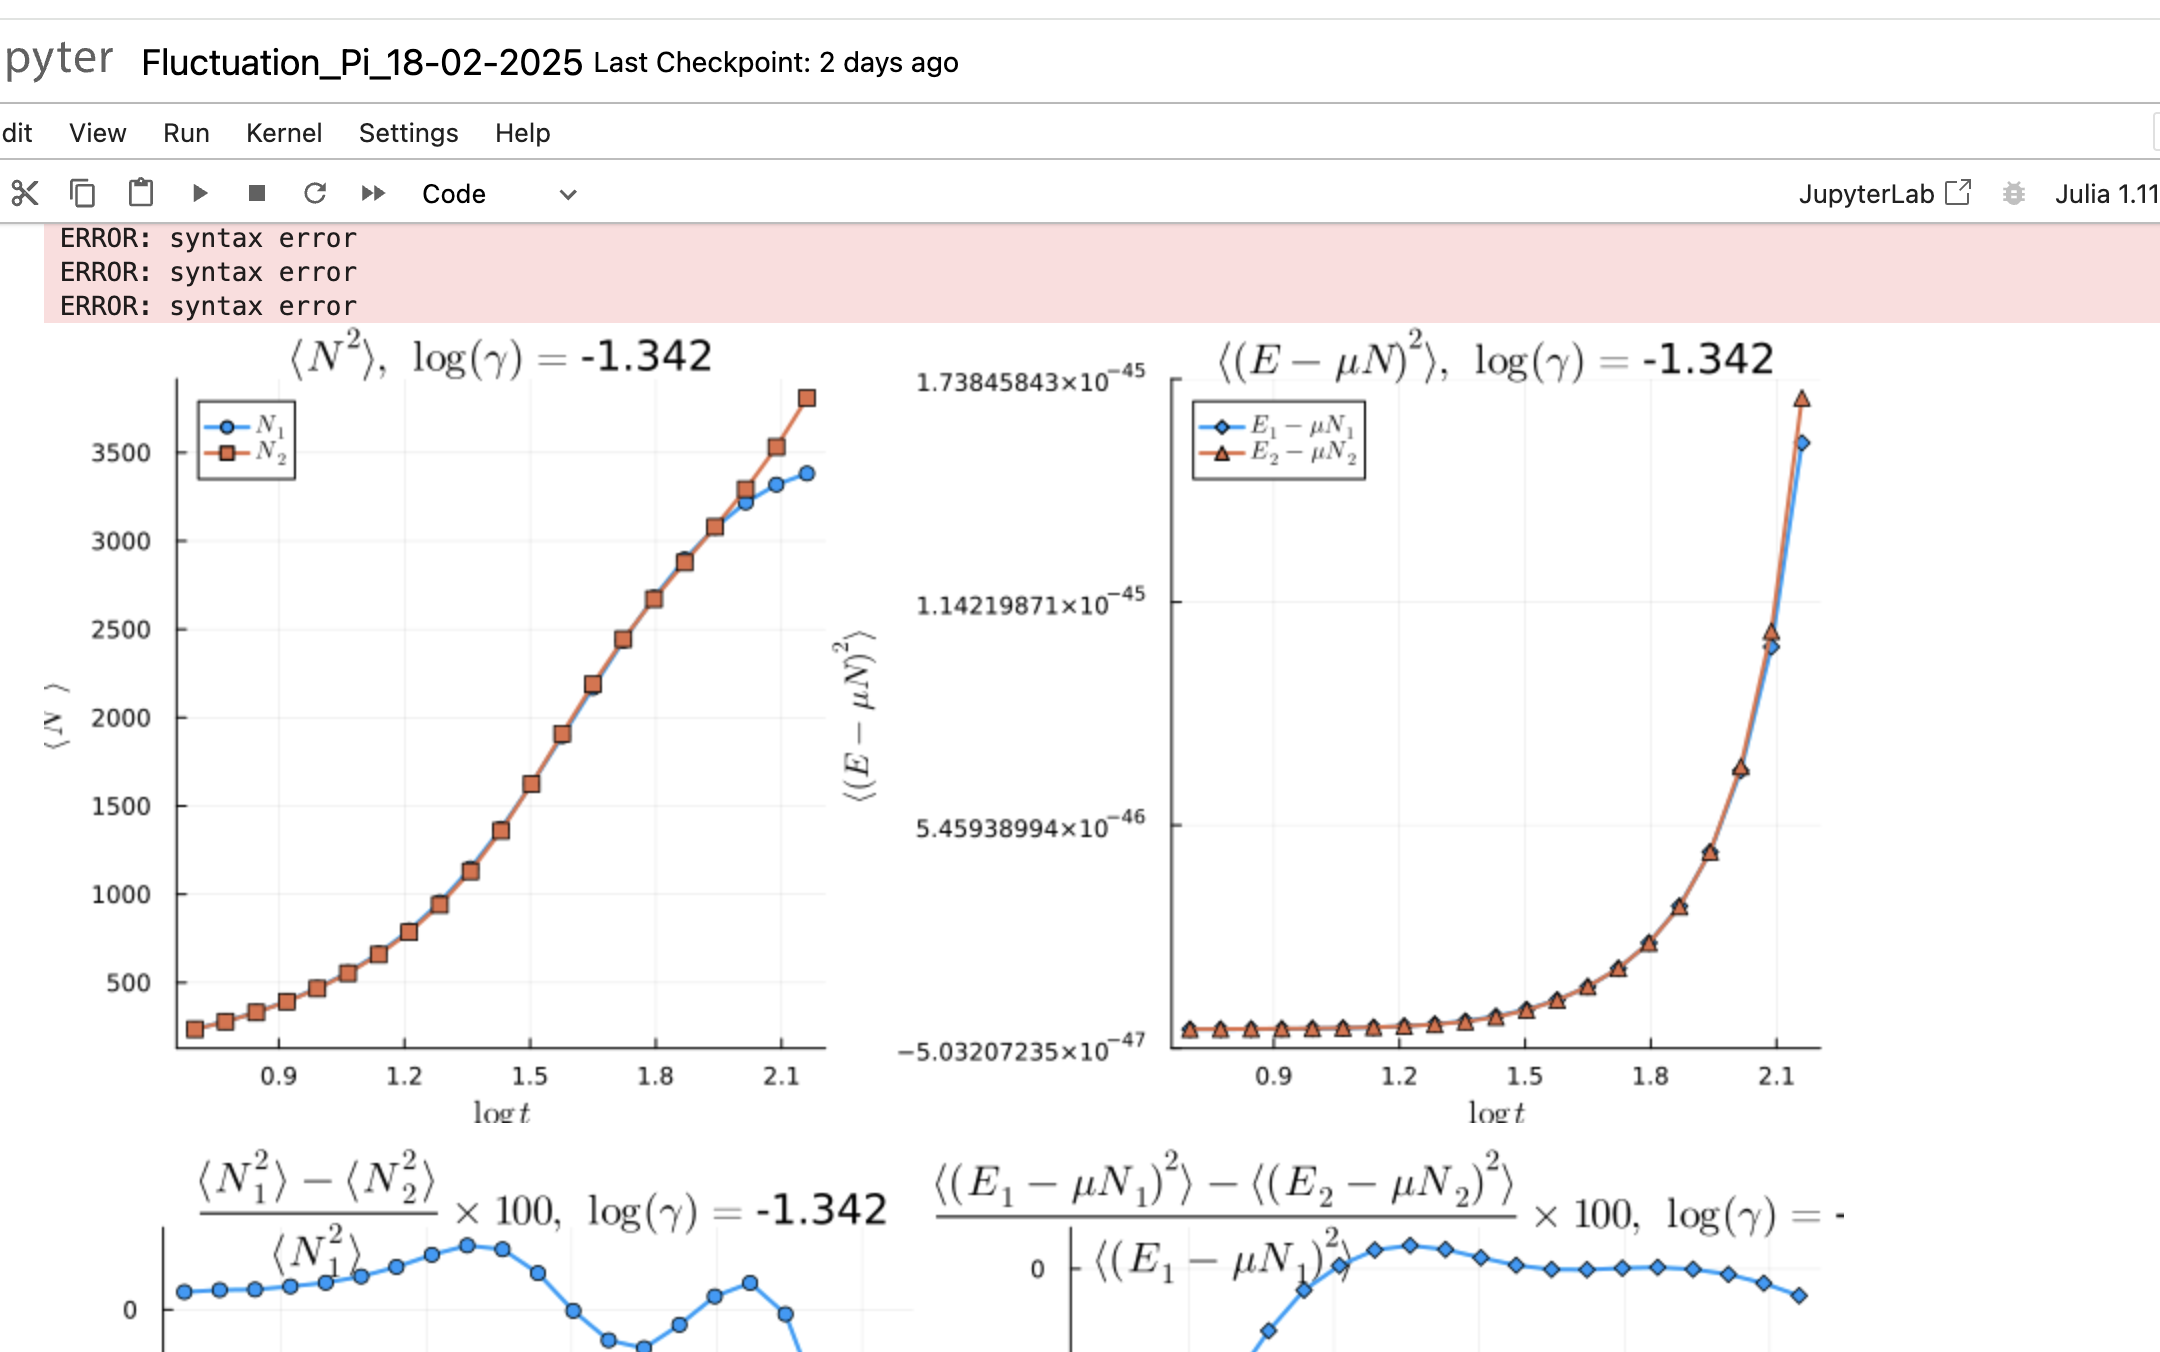
\includegraphics[width=1\textwidth]{Figures/test}

%\begin{aff}
%Donc une a l'ordre un en $\delta \theta (\operator{A}^{(0)})^{-1} %\operator{V}$ 

%\begin{eqnarray*}
%	\langle \delta \Pi ( \theta) \delta \Pi ( \theta') \rangle & = &  ( (\Pi^c_s - \Pi^c)\Pi^c/\Pi^c_s ) ( \theta ) \delta_{\theta, \theta'}/\delta \theta + \mathscr{F}(\theta , \theta' ) ,	
%\end{eqnarray*}

%avec 

%\begin{eqnarray*}
%	\mathscr{F}(\theta , \theta' ) & = & \left [ (\Pi^c_s - \Pi^c )( \theta)  +  (\Pi^c_s - \Pi^c ) ( \theta' )\right ] \frac{\Pi^c}{\Pi^c_s}(\theta)\frac{\Pi^c}{\Pi^c_s}(\theta') \frac{ \Delta( \theta'- \theta )}{ 2 \pi }\\
%	&&  - \left [ (\Pi^c_s - \Pi^c )( \theta)   (\Pi^c_s - \Pi^c ) ( \theta' )\right ] \frac{\Pi^c}{\Pi^c_s}(\theta)\frac{\Pi^c}{\Pi^c_s}(\theta')\int d\theta'' \left (   \frac{ \Pi^c/\Pi^c_s}{\Pi^c_s - \Pi^c} \right )(\theta'') \frac{\Delta(\theta''- \theta)}{2 \pi}\frac{\Delta(\theta''- \theta')}{2 \pi}  	
%\end{eqnarray*}
%\end{aff}



 








%%\section{Ordre 2 des corrections et rôle de l’entropie de Yang-Yang}
%%\section{Confrontation entre hydrodynamique classique et hydrodynamique généralisée}

\chapter{Protocoles experimentale}
\minitoc
\section{Présentation de l’expérience}

\subsection{Piégeage transverses et longitudinale}
\section{Outil de sélection spatial}
%%\section{Mesure de $\rho(x , \theta ) $ }

%\section{Mesure de distribution de rapidités locales $\rho(x , \theta ) $  pour des systèmes en équilibre}

\chapter{Étude du protocal de bi-partition : Mesure de distribution de rapidités locales $\rho(x , \theta ) $  pour des systèmes hors équilibre}
\minitoc
%%\section*{Abstract}
{\bf
Long wavelength dynamics of 1D Bose gases with repulsive contact interactions can be captured by Generalized HydroDynamics (GHD) which predicts the evolution of the local rapidity distribution. The latter corresponds to the momentum distribution of quasiparticles, which have infinite lifetime owing to the integrability of the 
system.
 Here we experimentally investigate the dynamics for an  initial situation that is the junction of two 
semi-infinite systems in different stationary states, a protocol referred to as `bipartite quench' protocol.
More precisely  we realise the particular case where one half 
of the system is the vacuum state. 
 We show that the evolution of the boundary density profile exhibits ballistic dynamics obeying the Euler hydrodynamic scaling. The boundary profiles are similar to the ones predicted with zero-temperature GHD in the quasi-BEC regime, with deviations due to non-zero entropy effects. 
 We show that  this protocol, provided the boundary profile is measured with infinite precision, permits to reconstruct the rapidity distribution of the initial state. 
 For our data, we extract the initial rapidity distribution by fitting the boundary profile and we use 
 a 3-parameter ansatz that goes beyond the thermal assumption. 
Finally, we investigate the local rapidity distribution inside the boundary profile, which, according to GHD, presents, on one side, features of  zero-entropy states. The measured distribution shows the asymmetry predicted by GHD, although unresolved deviations  remain. 
}



\section{Introduction} 
%[Permier jet : Isabelle]
\label{sec:intro}

Gaining insight on the out-of-equilibrium dynamics of many-body quantum systems is tremendously difficult and is the goal of an active research field.  
One particular class of systems where important progress has been made over the past decade is the class of integrable one-dimensional systems. 
Owing to their infinite number of local conserved charges, the description of the local properties of stationary states that arise after relaxation requires a whole function, the rapidity distribution~\cite{yang1969thermodynamics,zamolodchikov1990thermodynamic,rigol2007relaxation,mossel2012generalized,caux2012constructing,fagotti2013reduced,ilievski2016string}.
This function can be viewed as the velocity distribution of the infinite-lifetime quasi-particles in the system.   Its large-scale effective dynamics is described by  generalized hydrodynamics (GHD) \cite{bertini_transport_2016,castro-alvaredo_emergent_2016} (for recent reviews, see e.g.~\cite{bastianello2022introduction,doyon2025generalized}), which assumes local relaxation to a local stationary state.
As with any hydrodynamic theory, the most paradigmatic situation that can be handled by GHD is the `Riemann problem' \cite{riemann1860fortpflanzung}, also dubbed `bipartite quench' more recently~\cite{de_nardis_edge_2018,horvath2019hydrodynamics,alba2019entanglement,rylands2023transport,gamayun2023landauer,horvath2024full}, or `domain-wall quench' or `domain-wall protocol'~\cite{yuan2007domain,antal1999transport,hauschild2016domain,collura2018analytic,misguich2019domain,scopa2022exact,collura2020domain,scopa2023scaling,mcroberts2024domain}. In this `bipartite quench protocol', the microscopic dynamics is governed by a translation-invariant Hamiltonian but the initial state is the junction of two semi-infinite homogeneous systems each prepared in a different stationary state of the Hamiltonian. The GHD theory predicts that, at times long enough such that diffusion effects become negligible~\cite{de_nardis_diffusion_2019} and Euler-scale hydrodynamics is valid, the time evolution is ballistic. 
An interesting feature of this protocol is that the local state, within the merging region, is expected to present features characteristic of zero-temperature systems. Thus, this protocol could be used to reveal power-law singularities of correlation functions characteristic of a zero-temperature Luttinger liquid~\cite{de_nardis_edge_2018}, provided a local probe is used. 

In this paper, we experimentally realize an instance of the bipartite quench protocol using an ultra-cold atomic Bose gas, well described by the Lieb-Liniger model of one-dimensional Bosons with contact repulsive interactions\cite{lieb_exact_1963,bouchoule_generalized_2022}, which is an integrable model. 
In our experiment, the bipartition consists of the junction of a gas in a stationary state on one side, and the vacuum on the other side. This initial state is prepared by producing a homogeneous atomic cloud and by removing suddenly its left part. For different evolution times, we record the density profile of the boundary between the two regions, dubbed the boundary profile.  We find that the boundary profile exhibits a ballistic behavior, as expected from the predictions of GHD theory at the Euler scale. 

The boundary profile, for clouds prepared with deep evaporative cooling, is in fair agreement with GHD predictions assuming the semi-infinite gas is in its ground state, although deviations are present. From the boundary profile, we show that it is in principle possible to reconstruct the rapidity distribution characterizing the initial gas. This protocol can thus be used as a generalized thermometry. 
However, the reconstruction method suffers from a high sensitivity to experimental noise in the tail of the boundary profile, which prevents us from reconstructing faithfully the initial rapidity distribution. Instead, we use an ansatz parametrized by a few parameters to extract the rapidity distributions of the initial gas from a fit to the boundary profile. 

Finally, we use a newly developed technique \cite{dubois_probing_2024} to probe the local rapidity distribution within the boundary. The latter is expected to be highly asymmetric for an initial state whose rapidity distribution is substantially broader and 
smoother than that of the ground state: while one of its borders
reflects the broad character of the initial rapidity distribution, the other border
presents the sharp feature expected for the ground state. Our experimental data show such an asymmetric behavior, although the above feature is softened by the finite spatial resolution of the local rapidity distribution measurement.  


\section{Experimental setup}
%\subsection{Atom chip experiment}

We produce an ultra-cold gas of $^{87}$Rb bosonic atoms in the stretched state $|F=2,m_F=2 \rangle$ using an atom chip. In addition to a homogeneous longitudinal magnetic field $B_0 = 3.36 $G, transverse trapping is achieved with three parallel microwires deposited on the chip (shown in blue in Fig.\ref{fig:setup}(a)) which carry AC currents modulated at $400$MHz. This configuration eliminates wire roughness effects and allows independent control over both longitudinal and transverse confinement \cite{PhysRevLett.98.263201}. The atoms are trapped $7\mu$m from the chip surface and $15\mu$m from the wires, enabling strong transverse confinement. The transverse trapping potential is well approximated by a harmonic potential with a frequency of $\omega_{\perp}/ 2 \pi=2.56 $kHz for the data presented in this paper. 

Using radio-frequency evaporative cooling, we produce an atomic cloud at a temperature of approximately $T=100$nK and a chemical potential of $\mu/ k_B = 45$nK. With these parameters, $\mu/ (\hbar \omega_{\perp})=0.4$ and $k_B T/ (\hbar \omega_{\perp} )=0.8$, the gas enters in the $1$D regime. The effective 1D coupling constant for atoms in the transverse ground state is given by $g = 2 a_{3D} \hbar \omega_{\perp}$ \cite{PhysRevLett.81.938}, where $a_{3D}=5.3$ nm is the $3$D scattering length of $^{87}$Rb~\cite{PhysRevLett.89.283202}. Further details on the setup can be found in \cite{duboistel-04749900}. 
The dimensionless Lieb parameter $\gamma =  mg / (\hbar^2 n_0)$, where $n_0$ is the linear density, lies in the range $ [0.4,0.7] \times 10^{-2}$ and the  temperature fulfills 
$ T \ll n_0^{3/2} \sqrt{\hbar^2 g /m}/k_B$ such that the atomic clouds produced are deeply in the quasicondensate regime%, where density fluctuations are almost completely suppressed, but phase fluctuations remain 
\cite{PhysRevLett.91.040403}.




The longitudinal magnetic trap is produced by DC currents
running through four wires positioned on either side of the three microwires, as shown in the Fig.\ref{fig:setup}(a). Since these wires are placed far from the center of the chip, the longitudinal potential can be expressed as a polynomial series expansion $V(x)= \sum_{i} a_i x^i$. 
The fourth first coefficients $a_i$ are tuned by adjusting the currents in the four wires that generate the longitudinal trapping potential. By carefully selecting these currents, it is possible to set $a_1$, $a_2$ and $a_3$ to zero such that 
the leading term is  the quartic term $V(x)=a_4 x^4$. Such a potential permits to 

achieve a quasi-homogeneous atomic density over a relatively large region, an 
important feature to study the bipartite quench protocol which assumes 
a semi-infinite system.

An example of linear density profile for an atomic cloud placed in such a potential is represented in gray in Fig.\ref{fig:setup}(b). The linear density $n_0$ remains constant to within $10 \%$ around the peak density over a range of approximately $250 \mu$m. 



To produce the initial bipartition, we use the selection method introduced in \cite{PhysRevLett.133.113402}. We illuminate the left border of the atomic cloud, initially in a global stationary state in a quartic trap, with a pushing beam that is nearly resonant with the $F=2 \to F' = 3$ transition of the $D2$ line and which propagates perpendicularly to $x$. Atoms shined by this pushing beam are subjected to radiation pressure : after being illuminated for $30 \mu$s corresponding to $\sim 15$ absorption/reemission cycles, atoms
have enough energy to leave the trap. To illuminate only a border of the gas, the beam is shaped using a digital micromirror device (DMD). Further details on this spatial selection method are available in \cite{PhysRevLett.133.113402}. This protocol produces a sharp boundary between a zero density system and a quasi-homogeneous gas due to the fact that the atoms are initially placed in a quartic trap.  The sharpness of the boundary is mainly limited by the imaging resolution, which is in the micrometer range. The reabsorption of scattered photons by the atoms which are not shined could also limited the boundary sharpness. This effect is mitigated by detunning the pushing beam by $15$MHz from the D$2$ transition. An example of the density profile of a gas initially in a global stationary state in a quartic trap, after applying this spatial selection tool, is shown in yellow in Fig.\ref{fig:setup}(b).  %The gas is then homogeneous to within $10 \%$ over a distance of approximately $200 \mu$m. 

The longitudinal confinement is then removed while maintaining the transverse confinement. The initial sharp boundary broadens in time 
and this  dynamics is monitored by recording longitudinal density profiles $n(x,t)$ after different evolution time $t$. %to investigate the longitudinal dynamics.
\begin{figure}[!htb]
    \centering
    \includegraphics[width=0.90\linewidth]{Figures/Chip_selection_V2.pdf}
    \caption{%{\color{blue} Ah mince, je ne rélaise que maintenant que sur le dessin il n'y a que 2 fils gris et pas 4 ! Léa, tu as la source de la figure ? JE veux bien la modifier si tu n'as pas le temps.}
    (a) Schematic drawing of the atom chip. The $3$ blue wires produce the transverse trapping, the $4$ other wires produce the longitudinal trapping. The red oval ball represents the atomic cloud, trapped 12 microns above the wires {\color{blue} Je réalise que la figure a un nuage en rose clair qui n'est pas clair. Si c'est pas trop pénible, rependre la figure pour l'enlever ? } $-$ (b) {\color{blue} Linear density profiles extracted from absorption images.} The gray curve is the linear density profile of gas confined within a quartic potential. The atomic cloud is then illuminated during $30 \mu$s by a near resonant light beam, shaped using a DMD. The resulting density profile after a time of flight of $1$ms is depicted in yellow. }
    \label{fig:setup}
\end{figure}


\section{GHD predictions}\label{sec.GHDpredictions}
\label{sec:ghd}

The above experimental setup is described theoretically as follows. Under time evolution, the initial sharp boundary of the cloud gets smoother, and the time
derivatives of local quantities decrease. 
After some time, upon coarse-graining, one expects that the gas can locally be described by stationary states.

Stationary states of the Lieb-Liniger model are entirely characterized 
by their rapidity distribution $\rho(\theta)$.
Equivalently, they can be characterized by a function $\nu(\theta)$ dubbed `occupation factor' which takes values between 0 and 1, and which is related to  
the rapidity distribution $\rho(\theta)$ by
\begin{equation}
\nu(\theta)=\frac{\rho(\theta)}{\rho_s(\theta)} \mbox{, \qquad where \qquad } \rho_s(\theta)=
\frac{m}{2\pi \hbar} + \int \frac{d\theta'}{2\pi} \Delta(\theta-\theta') \rho(\theta') ,  \end{equation}
and $\Delta(\Theta)=2g/(g^2/\hbar+\hbar\Theta^2)$ is the `scattering shift' in the Lieb-Liniger model. The functions $\nu$ and $\rho$ are in one-to-one correspondence and in the following we use alternately $\rho$ or $\nu$. [For an introduction to this formalism, we refer to the lecture notes \cite{doyon2020lecture} or to Section 1 of the review article \cite{bouchoule_generalized_2022}.]

Since we assume local stationarity, the system as a whole is described by a time and position dependent rapidity distribution $\rho(x,t,\theta)$, or equivalently by the 
time and position-dependent occupation factor $\nu(x,t,\theta)$. The latter leads to simpler calculations, while the former is particularly useful to extract the linear density, which reads
\begin{equation}
    \label{eq:lineardensity}
n(x,t)=\int d\theta \, \rho(x,t,\theta)  .
\end{equation}


The GHD equations \cite{bertini_transport_2016,castro-alvaredo_emergent_2016} predict the time evolution of $\rho(x,t,\theta)$, or equivalently of $\nu (x,t,\theta)$. When written in terms of the occupation factor $\nu(x,t,\theta)$, the GHD equations take the form of a convective equation 
\begin{subequations}
\label{eq:GHD}
\begin{equation}
\frac{\partial\nu}{\partial t} + v^{\rm{eff}}_{[\nu]}\frac{\partial  \nu }{\partial x} = 0 ,
\end{equation}
and a second relation that fixes the effective velocity $v^{\rm{eff}}_{[\nu]}$ as a functional of the local rapidity distribution,
\begin{equation}
v_{[\nu]}^{\rm{eff}}(\theta) = \theta -\int  \Delta(\theta-\theta') \left (  v^{\rm{eff}}_{[\nu]}(\theta) - v^{\rm{eff}}_{[\nu]}(\theta') \right ) \rho(\theta') d\theta' .
\end{equation}
\end{subequations}
More precisely, Eq.~(\ref{eq:GHD}a) is the `Euler-scale' form of GHD, a diffusionless equation that is valid at the large scales. Diffusive corrections that enter in the form of a Navier-Stokes-type term~\cite{de2018hydrodynamic,de2019diffusion,bastianello2020thermalization,de2022correlation}, or even dispersive corrections~\cite{de2023hydrodynamic}, have also been studied theoretically. However, they are subleading and so far they have not been observed experimentally. We will see below that our experimental data obey the scaling collapse expected at the Euler scale (Fig.~\ref{fig:euler}), so these effects seem to be negligible in our situation, at least for the analysis of the boundary profiles. This is also compatible with a recent theoretical study in the weakly interacting regime that has concluded that diffusive effects should be very small~\cite{moller2024identifying}. Therefore, in this paper we ignore the possibility of subleading diffusive effects (as well as all higher-order effects) in our modeling, and we stick to the Euler-scale GHD equation above.

\begin{figure}[hbt]
    \centering
    \includegraphics[width=0.7\textwidth]{Figures/figure_nustar.pdf}
    \caption{Occupation ratio $\nu^* (v,\theta)$ solving the equation (\ref{eq:nuetoile}) for an initial occupation ratio $\nu_0 (\theta)$ in the right half-system corresponding to thermal equilibrium at temperature $T$. The dashed green line is the curve $\theta^*(v)$, {\it i.e.} it is the set of points $(v,\theta)$ such that $v^{\rm eff}_{[\nu^* (v,.)]} (\theta) = v$. [Parameters: 
    $\gamma_0=mg/(n_0\hbar^2)=0.005$, $k_B T \hbar^2/(mg^2) = 365$, close to the experimental parameters of the data sets below.]}
    \label{fig:nu_star}
\end{figure}

For an initial bipartition whose discontinuity is located at $x=0$, the solution of \eqref{eq:GHD} is invariant along rays of constant velocity $x/t$~\cite{bertini_transport_2016,castro-alvaredo_emergent_2016}. In other words, Eq.~\eqref{eq:GHD} implies that, for this class of initial states, 
the local occupation factor distribution, and thus all local properties of the gas,  depend on $x$ and $t$ only through the quantity $v=x/t$. The solution of Eq.~\eqref{eq:GHD} can thus be written 
using the occupation factor along rays $\nu^*(v,\theta)$ such that
\begin{equation}
\label{eq:nuvsnuetoile}
    \nu(x,t,\theta)=\nu^*( x/t,\theta).
\end{equation} 
%and solve Eq.~\eqref{eq:GHD}. 
For the situation considered in this paper with, initially, a vacuum state for negative $x$ and a state of occupation factor distribution $\nu_0$ one the right, 
 the solution $\nu^*(v,\theta)$ is parameterized by an edge rapidity $\theta^*$ according to~\cite{bertini_transport_2016,castro-alvaredo_emergent_2016}
\begin{equation}
\label{eq:nuetoile}
    \nu^*(v,\theta)=\left \{ \begin{array}{ccc} 
    \nu_0(\theta) &\mbox{ if }& \theta < \theta^*\\
    0 & \mbox{ if } & \theta > \theta^*\\
    \end{array} \right . \mbox{ where  \quad }  v^{\rm{eff}}_{[\nu^*(v,.) ]}(\theta^*)=v \, .
\end{equation}
%where $\theta^*$ is such that $v^{\rm{eff}}_{[\nu^*]}(\theta^*)=v$.
This equation can be solved numerically 
for any given initial distribution $\nu_0(\theta)$, see Fig.~\ref{fig:nu_star} for an example. Together with Eq.~\eqref{eq:nuvsnuetoile}, it entirely describes the system at the Euler scale. Note that, to compute the linear density $n(x,t)$ in order to compare with experimental density profiles,  one uses Eq.~(\ref{eq:lineardensity}).

\paragraph{Solution for a system initially in the ground state.}
To illustrate the above formalism, let us explore its implications for the special case where the right half-system is initially in the ground 
state. In that case the initial occupation factor $\nu_0 (\theta)$ is a Fermi sea: $\nu_0(\theta)=1$ for $|\theta| < \Delta\theta_0$, and $\nu_0(\theta)=0$ otherwise. The Fermi radius $\Delta\theta_0$ depends on the initial linear density $n_0$ through Eq.~(\ref{eq:lineardensity}) \cite{lieb_exact_1963}.

In that case the general features of the function $\nu^*(v,\theta)$ that solves the GHD equation (\ref{eq:GHD})  are as follows ( see Fig.~\ref{fig:boundary_profiles_theory}). It comprises three regions: an `empty region' far on the left with vanishing atom density, a `filled  region' far on the right where the density is equal to the initial density $n_0$, and a `central region' where the atom density interpolates between $0$ and $n_0$. It is easy to see that the left endpoint, where the atom density vanishes, is at $v= -\Delta\theta_0$. 
The right endpoint velocity on the other hand is the sound velocity in the fluid of density $n_0$, given by $c =v^{\rm eff}_{[\nu_0]} (\Delta \theta_0)$. %Thus

In the central region $ - \Delta \theta_0 < x/t < c$, the gas is locally in a state that is a Fermi sea shifted by a Galilean boost of velocity $V(x/t)$ for some function $V$. For arbitrary interaction strengths $g$ %the function $V(x/t)$ and 
the density profile $n(x/t)$ cannot be computed in closed form, but it is easily computed numerically. Analytical expressions are available in the two asymptotic regimes of strong and weak interactions which correspond to $\gamma\gg 1$ and $\gamma\ll1$ respectively.




\begin{figure}[thb]
    \centering
    \includegraphics[width=0.6\textwidth]{Figures/DWD_th_GS_V2.pdf}
    \caption{
    Boundary profile predictions from GHD for system initially in the ground state as a function of $\gamma$. The velocity  is normalized to the radius of the intial Fermi sea $\Delta \theta_0$. 
    On the negative side the 
    point where $n$ reaches 0 is at $\Delta \theta_0$ whatever $\gamma$.
    On the positive side, the point where $n$ reaches $n_0$ is at 
    the speed of sound $c$.
    The black, resp. grey, dashed line corresponds to the hydrodynamic prediction in the
    quasi-BEC regime (Eq.~\eqref{eq:GPE}), resp. in the  hard-core regime  (Eq.\eqref{eq:HS}).}
    \label{fig:boundary_profiles_theory}
\end{figure}


In the strong repulsion regime, or hard-core regime, 
$v^{\rm eff}_{[\nu]} (\theta)=\theta$ regardless of the occupation factor $\nu(\theta)$. Then 
Eq.\eqref{eq:nuetoile} is easily solved. 
We can use the fact that, in this regime, a Fermi sea of radius $\Delta\theta$ corresponds to a linear density $n=m\Delta\theta/(\pi\hbar)$ to derive

\begin{equation}
    (\gamma \gg 1) \qquad \qquad  n(x,t) \, = \, 
    \frac{n_0}{2}  \left( 1 +  \frac{xm}{t\pi\hbar n_0} \right)   \qquad {\rm if} \quad   -\pi\hbar n_0/m < x/t  < \pi\hbar n_0/m.
    \label{eq:HS}
\end{equation}

We can easily check that we recover the result expected for a gas of free fermions, as expected from the mapping of the hard-core bosons to fermions, which preserves the density\cite{girardeau_relationship_1960}. 
In the weakly interacting regime, or quasi-BEC regime, the effective velocity at the edge of a Fermi sea of radius $\Delta\theta$ is 
$\Delta\theta/2$, in the frame where the Fermi sea is at rest. Then, using the fact that, in this regime, a Fermi sea of radius $\Delta\theta$ corresponds to a linear density $n=m\Delta\theta^2/(4 g)$, we obtain

\begin{equation}
   (\gamma \ll 1) \qquad \quad  n(x,t)= 
    n_0 \left ( \frac{2}{3}+ \frac{1}{3} \frac{x}{ t}\sqrt{\frac{m}{gn_0}} \right )^2 \qquad  {\rm if} \quad  -2\sqrt{gn_0/m}   < x/t < \sqrt{gn_0/m}.
    \label{eq:GPE}
\end{equation}

Here we recover the hydrodynamic predictions derived from the Gross-Pitaevskii equation\cite{el_decay_1995,xu_dispersive_2017}. This is expected, since the Gross-Pitaevskii approach becomes exact in the limit of weak interactions, so it should agree with GHD, because GHD is the correct hydrodynamic equation for all repulsion strengths. 





In Fig.~\ref{fig:boundary_profiles_theory}, we compare the  GDH solution for 
systems initially in the ground state with the two above asymtotic formulas. We find that the quasi-BEC regime is reached to an excellent approximation already for $\gamma = 0.04$. 

\section{Experimental data}\label{sec.ed}


The boundary profiles for evolution times varying between $\tau = 10$ms and $\tau = 18$ms are shown in Fig.\ref{fig:euler}(a) and are represented as a function of $v=x /\tau$. The profiles overlap remarkably well, showing that the Euler scale is reached within this time interval. %experimentally observed for a deformation time from $\tau = 10$ms to $\tau = 18$ms. 
The longitudinal dynamics after $\tau = 18$ms cannot be probed due to the fact that our initial semi-homogeneous gas has a finite size. For shorter deformation times, experimental  boundary profiles  
are smoother than the Euler-scale GHD predictions, which might be due to
the failure of Euler scale, and/or to the 
fact that the cut at $t=0$ is not infinitely sharp. 
\begin{figure}[!htb]
    \centering
    \includegraphics[width=1.0\linewidth]{Figures/DWD_GPE_vs_exp_V2.pdf}
    \caption{(a) Boundary density profiles obtained for different evolution times $\tau$ and represented as a function of $x / \tau$ $-$ (b) Comparison of the boundary profile with the zero-temperature GHD prediction in the quasi-BEC regime Eq.\eqref{eq:GPE}. The latter 
    is an excellent approximation of the zero-temperature prediction for the interaction parameter of the data  which is $\gamma = 4.6\times 10^{-3}$ (see Fig. (3)). The edge profile in figure (b) is obtained after an expansion time of 10 ms and belongs to a different data set to those shown in figure (a). }
    \label{fig:euler}
\end{figure}

Fig.\ref{fig:euler}(b) compares  the  measured boundary profile $n(v)$ to the 
GHD prediction assuming that the initial state on the right is the ground state. Here the Lieb parameter is $\gamma = 4.6\times 10^{-3}$, and for such small values the boundary profile is indistinguishable from the quasi-condensate prediction, see Fig.\ref{fig:boundary_profiles_theory}, so we actually compare the data to Eq.~\eqref{eq:GPE}. 

The agreement between the ground state prediction and experimental data 
is rather good, especially in the high density part. 

The deviations from the parabola observed experimentally are  due to non-zero entropy effects, which are investigated  in the following section. 


\section{Retrieving the initial rapidity distribution from the boundary profile}

In Section~\ref{sec:ghd} we saw that, for a given initial occupation factor $\nu_0(\theta)$, we can compute the boundary profile $n(v)$ with the Euler-scale GHD equations. Since, in the experiment, we measure the boundary profile, it is natural to ask whether the converse operation is possible: Can we retrieve the occupation factor $\nu_0(\theta)$ from the boundary profile, relying on the Euler-scale GHD equations?


\paragraph{Direct reconstruction.}


We assume that we have a boundary profile $n(v)$ which is monotonically increasing, with $n(v) = 0$ when $v \rightarrow -\infty$, and $n(v) = n_0$ when $v \rightarrow +\infty$. 

A first idea is to reconstruct the function $\nu_0(\theta)$ incrementally, from negative values of $\theta$ to positive ones, by `reading' the boundary profile $n(v)$ from left to right. We can start from some highly negative velocity $v_0$, such that $n(v)$ is extremely small for all $v \leq v_0$ so it can be assumed to (numerically) vanish: $n(v) = 0$ for all $v \leq v_0$. We work with discrete values of the rapidities, with a constant spacing $\delta \theta > 0$, 
\begin{equation}
    \theta_j  =  v_0 + j \delta \theta , \qquad j \in \mathbb{N} ,
\end{equation}
and we reconstruct the corresponding values of the occupation factor $\nu_j$ ($\simeq \nu_0(\theta_j)$) inductively. We initialize the sequence as
\begin{equation}
    \nu_0 = 0 .
\end{equation}
At the $j^{\rm th}$ step, all the occupation factors $\nu_0, \nu_1, \dots, \nu_{j-1}$ are known, and we want to compute $\nu_j$. We fix $\nu_{j}$ by requiring that
\begin{equation}
%\left \{ \begin{array}{l}
    n (v_{j} ) \, = \, n_j , %\\
    %v_j = v^{\rm{eff}}_{[\nu^*(v_j,.)]}(\theta_j),
    %\end{array}\right .
    \label{eq:recursif}
\end{equation}
where $n(v)$ is the given boundary profile, and $n_j$ and $v_j$ are numerical estimates of the particle density and of the effective velocity respectively, obtained by discretizing the various integrals that enter the definitions of Section~\ref{sec:ghd}:
$$
n_j = \sum_{a=0}^j \frac{\delta \theta}{2\pi} \nu_a  1^{\rm dr}_{j,a} \quad  \left( \simeq \int^{\theta_j}_{-\infty} \frac{d\theta}{2\pi} \nu(\theta) 1^{\rm dr}(\theta) \right)
$$
$$
v_j = \frac{{\rm id}^{\rm dr}_{j,j}}{1^{\rm dr}_{j,j}}  \quad \left( \simeq \frac{{\rm id}^{\rm dr} (\theta_j)}{1^{\rm dr} (\theta_j)} \right) .
$$
Here ${\rm id}(\theta) = \theta$ is the identity function, and the discretized dressed function $f^{\rm dr}_j$, for a function $f$, is the solution of the linear system
$$
f^{\rm dr}_{j,a} = f (\theta_a) + \sum_{b=0}^j \frac{\delta \theta}{2\pi} \Delta(\theta_a - \theta_b) \nu_b  f^{\rm dr}_{j,b} .
$$
This is the discrete analog of the definition of the dressing, which is the solution of the integral equation $ f^{\rm dr}(\theta) = f(\theta) + \int_{-\infty}^{\theta_j} \frac{d\theta'}{2\pi} \Delta (\theta-\theta') \nu(\theta') f^{\rm dr}(\theta') $ [see e.g. Refs.~\cite{doyon2020lecture,bouchoule_generalized_2022} for introductions to this formalism]. The value of $\nu_j$ that fulfills Eq.\eqref{eq:recursif} can be found numerically with a root-finding algorithm; we use the bisection method.



In the limit of small spacing $\delta \theta$, this procedure is expected to converge to a continuous occupation factor $\nu_0(\theta)$. We have tested this method starting with the boundary profiles corresponding to some known occupation factors, and verified that it reconstructs the correct occupation factor $\nu_0(\theta)$ as expected.


However, when we try to apply this method to experimental boundary profiles, we face two difficulties. First, from spares  and noisy experimental data points one needs to extract an increasing continuous function $n(v)$. For this, we need to fit the data with some ansatz for the boundary function. Second, we have observed that this method is highly sensitive to the details of the boundary profile $n(v)$, especially to the left tail of $n(v)$ at negative values of $v$. Since the signal-to-noise ratio in our experimental data is poor in this region, the results obtained with this technique are not trustworthy. Thus, we prefer to use an alternative method, which we present now.

%{\color{blue} Il faut d'abord faire un fit pour avoir une fonction strictement croissante et que l'on connait en tout point.}However, we have observed that it is highly sensitive to the details of the boundary profile $n(v)$, especially to the left tail of $n(v)$ at negative values of $v$. Since the signal-to-noise ratio in our experimental data is poor in this region, the results obtained with this technique are not trustworthy.


%\begin{eqnarray}
%\nonumber   A [\nu] (\theta^*)  &  \overset{{\rm def}}{=} & 	\frac{\delta ( v^{\rm eff}(\theta^*) )}{\delta \theta^*} \\
%&=& \frac{1}{1^{\rm dr} (\theta^*)}  \left( 1 + \int_{\theta^*}^\infty \varphi'(\theta^* - \theta) [ {\rm id}^{\rm dr}(\theta) - v^{\rm eff}(\theta^*) 1^{\rm dr}(\theta)  ]  \nu(\theta) \frac{d\theta}{2\pi} \right) 
%\end{eqnarray}
%and $D [\nu] = A[\nu] / B[\nu]$ with
%\begin{eqnarray}
%  \nonumber   B[\nu] (\theta^*) \, \nu (\theta^*) &  \overset{{\rm def}}{=} & 
%\frac{ \delta ( n(\theta^*) ) }{\delta \theta^*} \\
% &=& - \frac{1^{\rm dr} (\theta^*)^2}{2\pi}    \, \nu (\theta^*)   \, .
%\end{eqnarray}
%$A$, $B$ and $D$ are functionals of $\nu$ whose functional derivatives $\frac{\delta A}{\delta \nu (\theta)}$, $\frac{\delta B}{\delta \nu (\theta)}$, $\frac{\delta C}{\delta \nu (\theta)}$ are smooth at $\theta = \theta^*$.
%Let us define $D [\nu] = A[\nu] / B[\nu]$ so that
%\begin{equation}
%	\nu (\theta^*) \, = \, D[\nu](\theta^*) \frac{dn}{dv} .
%\end{equation}
%Differentiating w.r.t $\theta^*$, this gives Eq.~(\ref{eq:dndtheta}).

%This can then be used in the form of the following algorithm. Formula (\ref{eq:dndtheta}) can be used to reconstruct the rapidity distribution if we know the velocity function $n(v)$. We work on a finite grid in rapidity space,
%\begin{equation}
%	\theta_j = \theta_0 + j \, \Delta \theta , \qquad j = 0, \dots, N.
%\end{equation}
%We define
%\begin{equation}
%	A_N = 1,  \qquad  A_{N-1} = 1, \qquad D_N = -2\pi , \qquad D_{N-1} = - 2\pi ,
%\end{equation}
%and
%\begin{equation}
%	v_N = \theta_N,  \qquad  v_{N-1} = \theta_{N-1} , \qquad   \nu_N = 0,  \qquad  \nu_{N-1} = 0. 
%\end{equation}
%Then we compute everything inductively as follows. At each step we define the new velocity
%\begin{equation}
%	v = v_{j+1} - A_{j+1}  (\theta_{j+1} - \theta_j) ,
%\end{equation}
%then we evaluate $dn/dv$ and $d^2 n/dv^2$ at this velocity, and then
%\begin{equation}
%	\nu_j = \nu_{j+1} -  ( D_{j+2} - D_{j+1} ) \frac{dn}{dv} -    A_{j+1} D_{j+1} (\theta_{j+2} - \theta_{j+1})  \frac{d^2 n}{d v^2} .
%\end{equation}
%Then we use the values $\nu_j, \nu_{j+1}, \dots, \nu_N$ as an estimate of the function $\nu(\theta)$ and we compute
%\begin{equation}
%	v_j = v^{\rm eff}(\theta_j) , \qquad  A_j = A[\nu](\theta_j) , \qquad  D_j = D[\nu](\theta_j) .
%\end{equation}




%\textit{Transition :} 

%\subsection{Using GHD equations}

%\begin{itemize}
%    \item Thermal ansatz
%    \item Non thermal ansatz
%\end{itemize}

%\subsection{Fitting the occupation factor $\nu_0(\theta)$}
\paragraph{Fitting the occupation factor $\nu_0(\theta)$.}


%Extracting $\nu_0 (\theta)$ remains unattainable it amounts to  determine an infinite number of fitting parameters  with a data set of finite dimension and moreover plagged by noise.
In order to extract the occupation factor distribution $\nu_0 (\theta)$, we fit the experimental boundary profile with the GHD calculations based on Eqs.~(\ref{eq:nuvsnuetoile})-(\ref{eq:nuetoile}). Extracting $\nu_0(\theta)$ exactly would correspond to a fit with infinitely many fitting parameters, which we are not able to do. So we choose an Ansatz for $\nu_0(\theta)$, parameterized only by a few fitting parameters.


\begin{figure}[!htb]
    \centering
    \includegraphics[width=1.0\linewidth]{Figures/nu_th_vs_s_V3.pdf}
    \caption{%{\color{blue} Inverser (a) et (b) sur les figures, je trouve ça plus logique.} 
    (a) The experimental boundary profile plotted in yellow is compared to fitted profiles using
    for $\nu_0(\theta)$ either  a thermal ansatz, {\it i.e.} the solution of Eqs.~\eqref{eq:fonctions} and  \eqref{eq:stherm}, (black dashed line) or the three-parameters ansatz defined by Eqs.\eqref{eq:fonctions} and \eqref{eq:s} (red line). (b) Comparison of the occupation factors obtained for both fitted 
    occupation factor distributions. 
%    after fitting the experimental boundary profile using a thermal ansatz $\nu(T,\mu)$ on the one hand and, and, on the other hand, an ansatz where $\nu$ solves Eq.\eqref{eq:fonctions} with the function $s$ given by Eq.\eqref{eq:s}.   }
}
    \label{fig:fitted_border}
\end{figure}


The first ansatz that we try is the occupation factor of a Gibbs ensemble, where the fitting parameters are the temperature $T$ and the chemical potential $\mu$. This was calculated first by Yang and Yang~\cite{yang1969thermodynamics}, who showed that the occupation factor $\nu(\theta)$ is the solution of the integral equation
\begin{equation}
\label{eq:fonctions}
     s'(\nu(\theta)) =  \frac{\mu}{k_B T} -\frac{m\theta^2}{2k_B T}  + \int d\theta' \Delta(\theta-\theta')
    \left [ s(\nu(\theta')) - \nu(\theta')s'(\nu(\theta)) \right ]
\end{equation}
where the function $s:[0:1]\rightarrow {\mathbb R}$ is
\begin{equation}
    s(y)=  -\left( y\ln(y) +(1-y)\ln(1-y) \right ),
  \label{eq:stherm}
\end{equation}
and $s'$ is its derivative. The integral $\int s(\nu(\theta))  
\rho_s(\theta) d\theta $ is the entropy per unit length of the occupation factor distribution $\nu(\theta)$~\cite{yang1969thermodynamics}.
For a given $T$ and $\mu$, Eq. \eqref{eq:fonctions} can be solved numerically iteratively very efficiently using the fact that 
$s'^{-1}(\epsilon)=1/(e^{-\epsilon/(k_{\rm B} T)}+1)$.
%the solution of $s'(\nu)=\epsilon$ is $\nu=1/(e^{-\epsilon/(k_BT)}+1)$. Once we have the occupation ratio $\nu_0(\theta)$, we use Eqs.~(\ref{eq:nuvsnuetoile})-(\ref{eq:nuetoile}) to compute the corresponding boundary profile.



In Fig.~\ref{fig:fitted_border} we compare the experimental boundary profile with the best fit obtained from this thermal equilibrium ansatz. For the data set shown here, the fitted temperature and chemical potential are 
$T=282$nK and $\mu / k_{\rm B}=71.5$nK. 
The fit is quite good although we see some discrepancies: the left tail of the experimental data is wider than that of the fit while on the right side, the experimental date are more sharp. Such a behavior is seen on all our data sets.


The discrepancy between the thermal fit and the experimental boundary profile may 
indicate the fact that the initial cloud, which is in a global stationary state in the quartic potential, is not in a thermal equilibrium state.
%{\color{blue} Dire que le nuage est stationnaire --> }
Global stationarity is supported by the fact that the density profile of the trapped cloud is time-independent. 
General stationary states of the GHD equations in presence of a confining potential $V(x)$ have a local occupation 
factor distribution $\nu(x,\theta)$ which obeys Eq.~\eqref{eq:fonctions} with a global 
'temperature' $T$ and a local 'chemical potential' $\mu(x)=\mu_0 -V(x)$, where $\mu_0$ is the central chemical potential. However, general stationary states differ from thermal states by the choice of the 'entropy' function $s(y)$, which does not need to be given by  Eq.\eqref{eq:stherm}, but can be an arbitrary function~\cite{Bulchandani23}. In the following %, to fit the boundary profiles, 
we generalize the 
thermal stationary state by modifying the function $s$ as follows,
%: we consider occupation factors $\nu$ that solve Eq.\eqref{eq:fonctions} but with an `entropy' $s$ function of the form
\begin{equation}
    s(y)=  -(1+cy)\left( y\ln(y) +(1-y)\ln(1-y) \right ) ,
    \label{eq:s}
\end{equation}
where $c$ is a third fitting parameter (together with the `temperature' $T$ and the `chemical potential' $\mu$), which is vanishing 
for thermal states. More precisely, we fit the experimental boundary profile %data 
with the prediction for 
an initial  occupation factor $\nu_0$ which is the one which obeys Eq.~\eqref{eq:fonctions} with the above function $s$.
%a thermal state corresponding to the case $c=0$. %The parameters $\mu,T$ and $c$ are used as fitting 
%where we use the numbers $\mu,a$ and $b$ are fitting 
%parameters.
  %corresponds to a thermal ansatz.
A fit of our data with this ansatz gives $\mu/k_B=74$nK, $T/k_B=480$nK and 
$c=2.92$. This fit decreases the square distance
to the data by  $30$ \% compared to the thermal fit.



\section{Probing the local rapidity distribution}
%{\bf [Premier jet : Guillaume]}
\label{sec:local}

For an initial state of the gas corresponding to a smooth occupation factor $\nu(\theta)$ ---for instance a thermal state---, the occupation factor  $\nu^*(x/t,\theta)$ at fixed ratio $x/t$ is expected to be highly asymmetric as a function of $\theta$, according to Eq.\eqref{eq:nuetoile}. Indeed, on the left side it has a jump discontinuity, similar to the one of the ground state occupation function, while on the right side it is smooth. To reveal such peculiar features of the local state of the gas, we use the protocol introduced in Ref.~\cite{dubois_probing_2024} to probe the local rapidity distribution, as we explain next.
		
		First, we let the gas expand for a time $t=18 \mbox{ ms}$, such that the boundary broadens and covers a large zone of $\sim 350 \mu$m, see Fig.~\ref{fig:simul_deformation}(a).
		%{\color{blue}[Il faudra un graphe avec le profil de bord à 18ms pour ces données pour pouvoir visualiser ce que représente 37 $\mu$m.]} 
		Then we select the slice of the gas that lies in an interval  $[x_0-\ell/2, x_0+\ell/2]$, removing all atoms lying outside the slice with a pushing beam~\cite{dubois_probing_2024}.
		In Fig.~\ref{fig:simul_deformation}(a) we show the density profile $1$ms after the selection of the slice.
		The fit to a smoothened rectangular  function gives $x_0= 18\,\mu$m.
		For calculations, the width $\ell$ will be determined using the 
		number of selected atoms (see below).
		Finally, we let this slice expand in 1D for an expansion time $\tau$, and then we measure the longitudinal density $\tilde{n}(x, {\tau} )$.  The latter reflects the total rapidity distribution of the slice $\Pi(\theta)=\int_{x_0-\ell/2}^{x_0+\ell/2}  \rho(x,\theta) dx$, because the asymptotic behavior as $\tau\rightarrow \infty$ is $ %\underset{\tau\rightarrow\infty}{\lim} 
		\tau \tilde{n}(x, {\tau} ) \simeq \Pi((x-x_0)/\tau)$.  The 
		expected asymmetry of $\Pi$ is thus expected to induce an asymmetry of the density $\tilde{n}(x,\tau)$ as a function of the position $x$. We observe this asymmetry experimentally in our expansion profiles, as expected. This is shown in Fig. \ref{fig:simul_deformation}~(b) for an expansion time of $\tau=30~\mbox{ms}$.
		
		\begin{figure}[!htb]
		
		\end{figure} 
		
		\begin{figure}[!htb]
		
		\begin{tikzpicture}
            % Première image avec une légende à l'intérieur
            \node[rectangle, draw = none] (bord) at (0,0) {                \includegraphics[width=0.5\textwidth]{Figures/article_simul_deformation_1_24-04-2024-T-x0}
            };
            \node[circle, draw=none, above=0cm of bord , shift={( -2.5cm , -0.5cm )} ] {(a)};
    
            % Deuxième image à droite de la première avec un décalage de 1cm
            \node[right=1mm of bord , shift={( -0.5cm , 0cm )}] (assy) {
              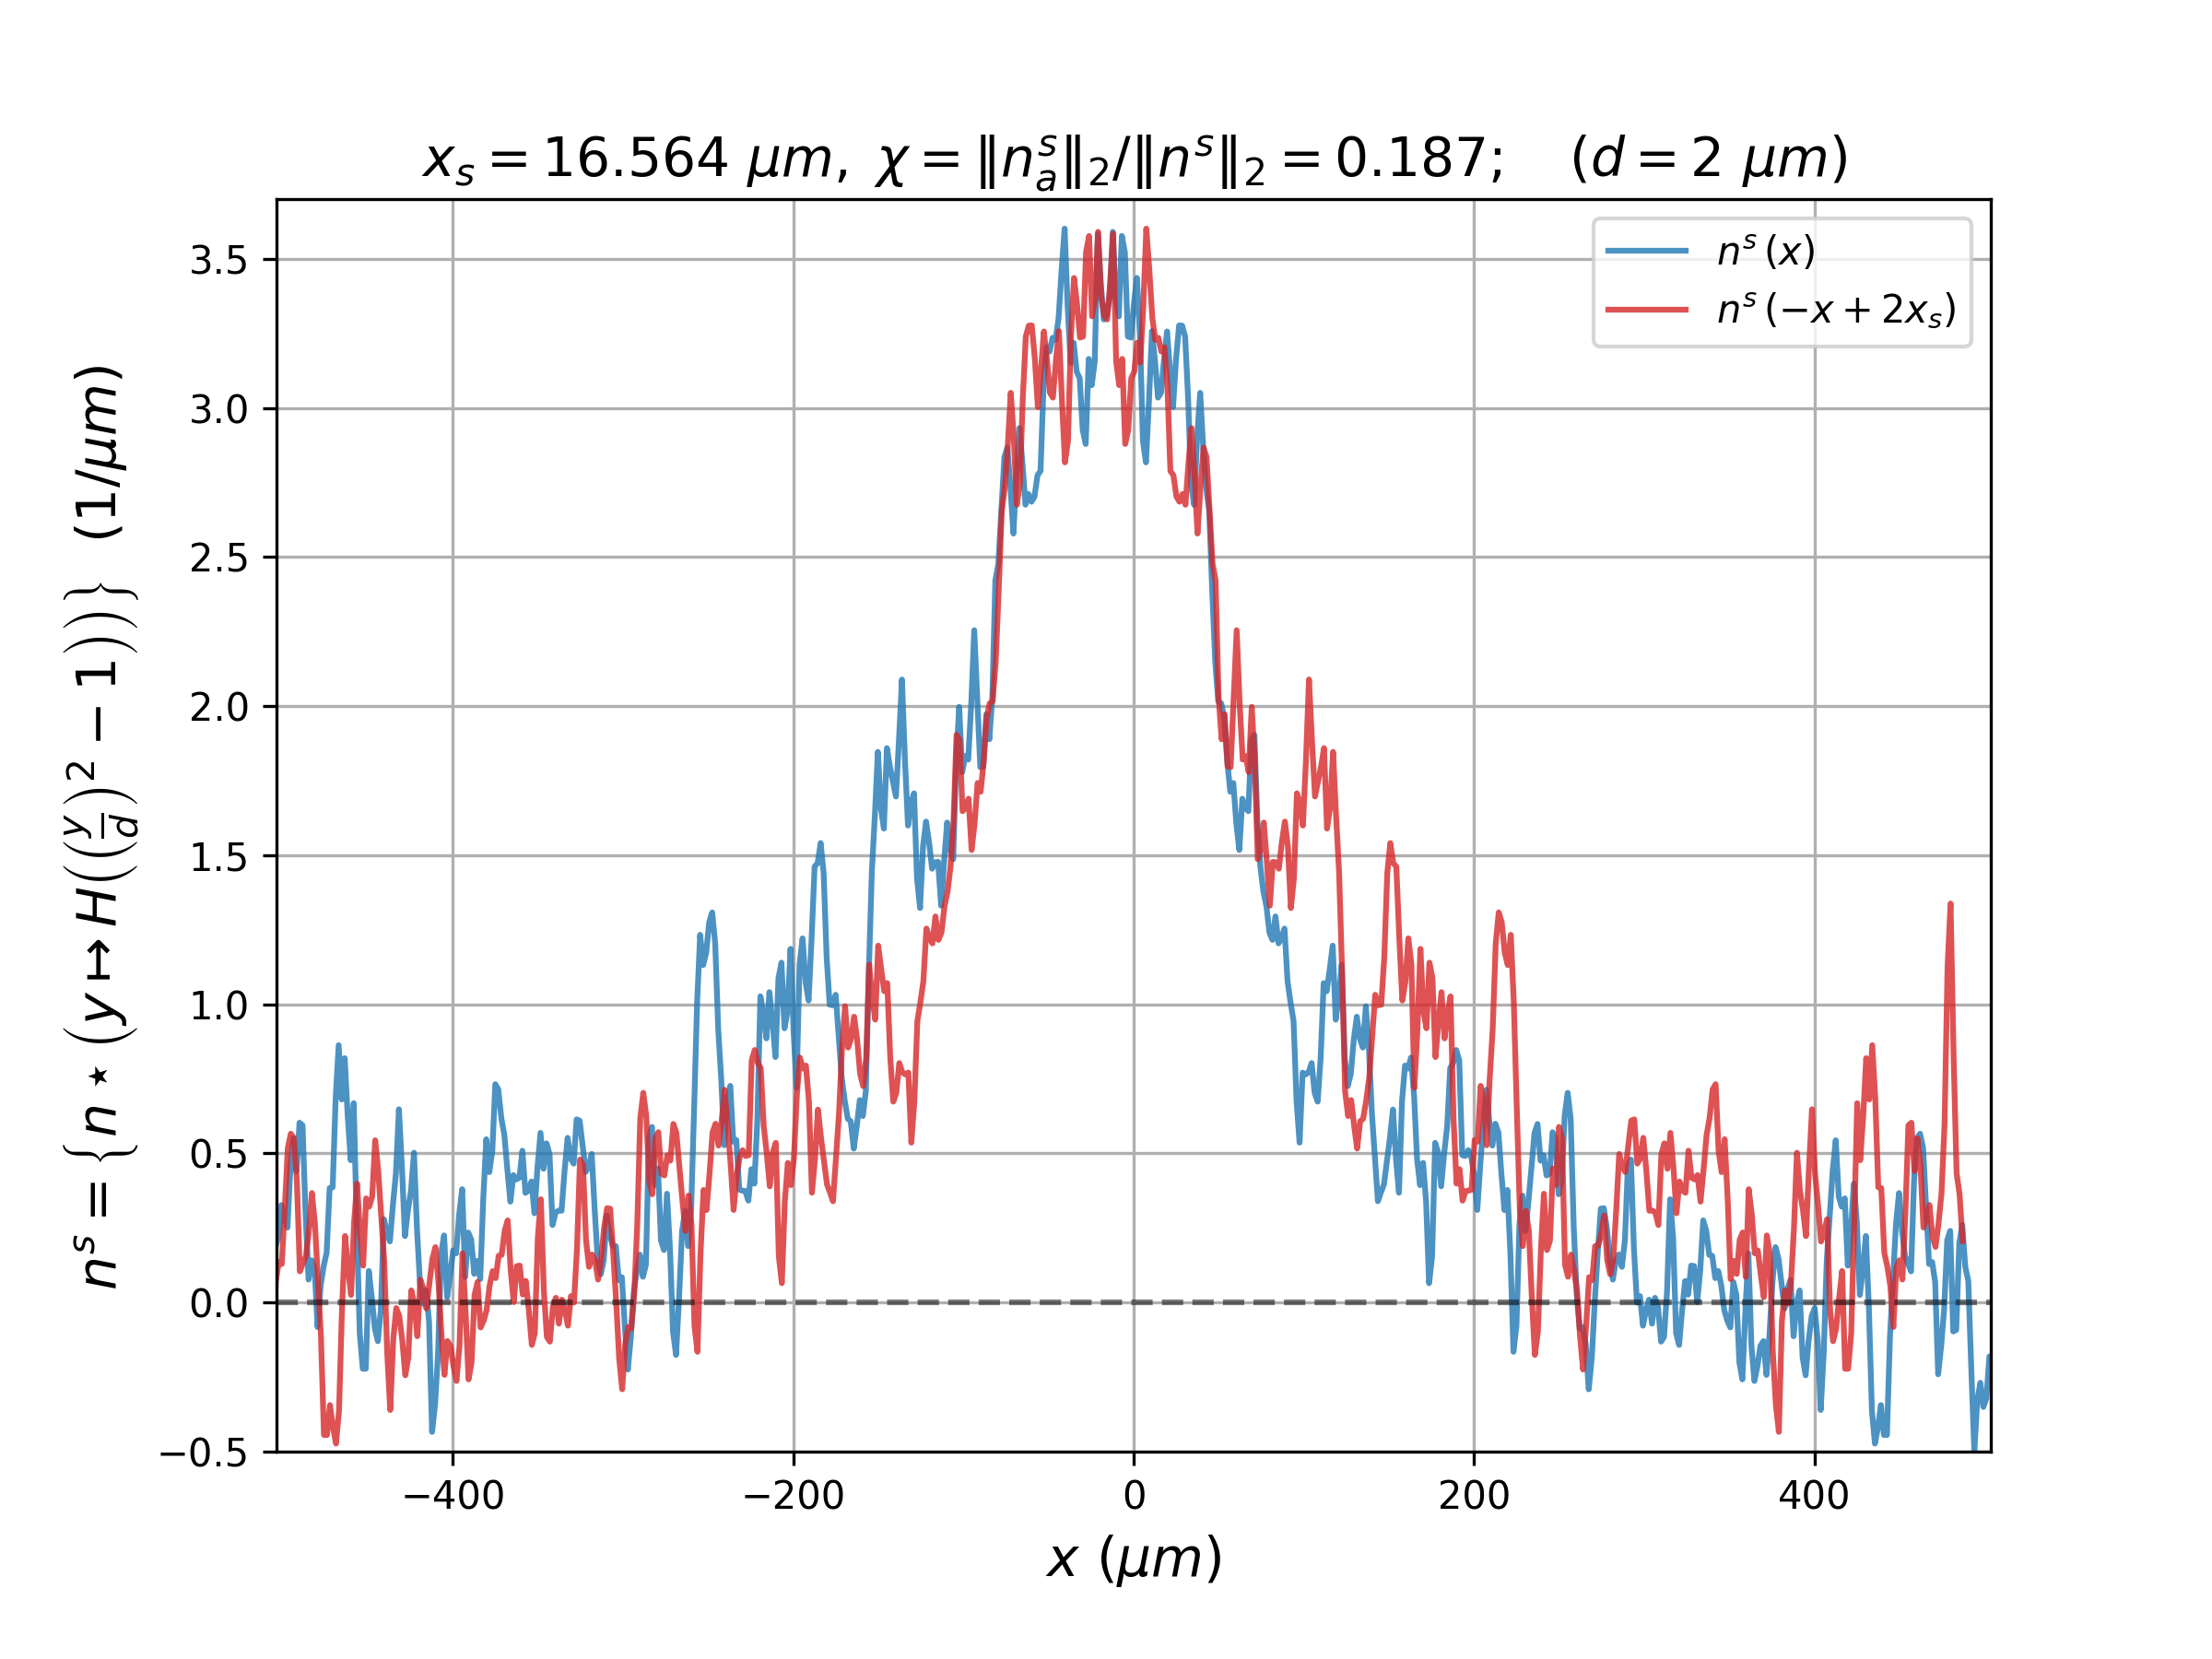
\includegraphics[width=0.5\textwidth]{Figures/article_asymetrie_24-04-2024}
            };
            \node[circle, draw=none, above=0cm of assy , shift={( -2.5cm , -0.5cm )}] {(b)};
        \end{tikzpicture}
        			\caption{%{\color{blue}(Donnée du 24-04-2024) }
        			(a). {\it Boundary profile and selected slice.} The boundary profile after $18\,ms$ evolution time is shown in solid yellow line. A thermal fit yielding $T=560\,nK$ is shown in orange.  The density profile taken $1\,ms$ after the slice selection is shown in blue. (b).  {\it Asymmetry of the slice expansion profile.} The density profile after an expansion of the slice aver a time $\tau=30$ ms is compared to its miror image. The symmetry center $x_s= -17\,\mu$m is the point that minimises the curves square distance $\delta^2=\int dx (\tilde{n}(x)-\tilde{n}(2x_s -x))^2$.  
        			}
        		\label{fig:simul_deformation}
        		
   			\end{figure} 
   		
		
		To go beyond this qualitative observation, we perform an Euler-scale GHD calculation
		of the expansion profile, assuming that the initial state is thermal. We extract the temperature by fitting the boundary profile before the selection of the slice, as shown in Fig. 6(a),  
        yielding $T=560$ nK.
        The chemical potential is adjusted so that the initial linear density is the linear density
        in the region $x>0$ measured before the boundary broadening.
		  Starting from the initial sharp profile, we simulate both the boundary broadening and the slice expansion with GHD, assuming a perfect slicing, i.e. $\nu(x,\theta)=0$ if $|x-x_0|>\ell/2$ and $\nu(x,\theta)$ is unchanged if $|x-x_0|<\ell/2$. The slice width $\ell$ is adjusted so that the calculated number of selected atoms equals  
		 the number of atoms in the experimental expansion profile, and we find $\ell= 24 \,\mu$m. %{\color{blue} JE ne comprends pas, il y a quelques jours c'était 18 $\mu$m ??? Et aussi, on était embêté car c'était assez différent du $\ell$ déduit de la courbe bleue de la figure 6(a) (de mémoire un facteur 1.4). C'est pourquoi on utilise cette méthode tordue.  Or là tout d'un coup, ce $\ell$ est très proche du $\ell$ déduit de la courbe bleue de la figure 6(a). Du coup, c'est con de faire comme ça ! BOn tant pis. }{\color{olivegreen} Sans cette methode on a $\mu$ , $T$ abérant et les nombre d'atome est différent de 20$\%$ (je donne plus de details dans le document \texttt{Figures/Donnees\_bord\_reponse\_28\_02\_2025.pdf}
%} 
		 %{\color{blue}Which is 1.4 times smaller than the half-width at half-maximum of the profile after $1~$ms of expansion.} {\color{blue} Et alors ? Comparé à la largeur à mi-hauteur du profil bleu de la figure 6(a) ?}
		 % {\color{blue}{ for we find a slice width $\ell=18\,\mu$m}}. 
		 %{\color{blue} MAis alors $\ell$ dépend de $T$ non ? Donc on ne peut pas dire $\ell=18~\mu$m.}
		%The  temperature of the initial state, $T=560$ nK, is 
		%obtained by fitting  the boundary profile, as shown in Fig.~\ref{fig:simul_deformation}(a).    
		The simulated expansion profile is shown in Fig.~\ref{fig:simul_expansion}(a). It displays a strong asymmetry, as expected, with a sharp right edge and a vanishing density beyond a certain point on the right. The sharpness of this edge is, however, less pronounced than the one expected for the local rapidity distribution $\rho(x_0,\theta)$ at $x=x_0$, see Fig.~\ref{fig:simul_expansion}(a). Two effects contribute to the broadening of  the  edge. First the rapidity distribution is not homogeneous inside the slice and $\Pi(\theta)$ differs from $\ell \rho(x_0,\theta)$, as seen comparing the 
		solid brown line and dashed line in Fig.\ref{fig:simul_expansion}~(a). Second, the expansion time is finite and the expansion profile is not exactly $\Pi((x-x_0)/\tau)/\tau$, as seen comparing the 
		red  and brown  solid lines in Fig.\ref{fig:simul_expansion}~(a).
		
		\begin{figure}[!htb]
		
		\begin{tikzpicture}
            % Première image avec une légende à l'intérieur
            \node[rectangle, draw = none] (exp) at (0,0) {
                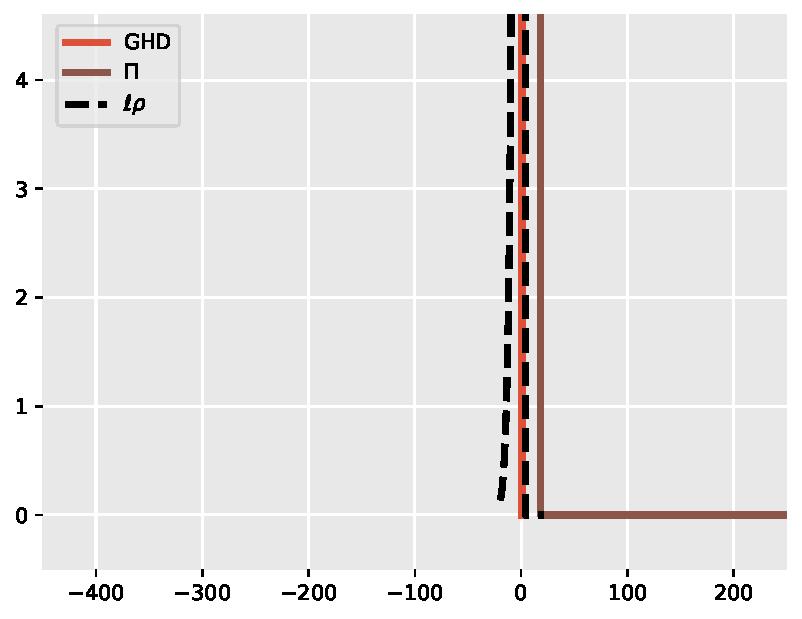
\includegraphics[width=0.5\textwidth]{Figures/article_distribution_24-04-2024}
            };
            \node[circle, draw=none, above=0cm of exp , shift={( -2.5cm , -0.5cm )} ] {(a)};
    
            % Deuxième image à droite de la première avec un décalage de 1cm
            \node[right=1mm of exp , shift={( -0.5cm , 0cm )}] (pi) {
                \includegraphics[width=0.5\textwidth]{Figures/article_simul_expansion_1_24-04-2024-T-x0.pdf}
            };
            \node[circle, draw=none, above=0cm of pi , shift={( -2.5cm , -0.5cm )}] {(b)};
            
        \end{tikzpicture}
    	
    		\caption{(a) {\it Density profile after slice expansion: effects of finite slice width and finite expansion time.} Orange line:  GHD calculation of the density profile after an expansion of the  slice for $\tau=30$~ms, using as the initial temperature the value $T=560$~nK obtained fitting the boundary profile.  The brown  line
    		is the expected distribution if one 
    		assumes that the asymptotic large expansion time is reached, {\it i.e.} it shows
    		 $\Pi((x-x_0)/\tau)/\tau$, where  $\Pi(\theta)=\int_{x_0-\ell/2}^{x_0+\ell/2} \rho(x,\theta) d x$ is the rapidity distribution of the selected slice. %, computed here just before the slicing. 
    		The  black dashed line is $\ell \rho(x_0, (x-x_0)/\tau)/\tau$, which is the expected result in the limit of large $\tau$ and for a slice width $\ell$ negligible compared to the boundary extension. %so that $\Pi(\theta)\simeq\ell \rho(x_0,\theta)$.
    		(b) {\it Comparison to experimental data.} Experimental data obtained after slice expansion during $\tau=30$ ms (blue line) is  compared to GHD calculations assuming an initial thermal state. 
    		 The  orange line, which is the same as in Fig.(a), is done for the temperature  $T=560 $nK, obtained by a fit of the boundary profile. The magenta line is a fit of the experimental expansion profile yielding $T=1550$ nK.
    		}
   			\label{fig:simul_expansion}					
		\end{figure}
		

		
		Next, we compare the expansion profile simulated with GHD to the experimental data.
		As shown in Fig~\ref{fig:simul_expansion}(b), the  predicted profile reproduces the main features of the  experimental expansion profile. Discrepancy are however as large as 25\% in the central part of the profile. In an attempt to get a better agreement between data and calculations, we fitted the experimental expansion profile with the GHD calculation using the temperature of the initial state as a fitting parameter. The result, shown as magenta line in Fig.\ref{fig:simul_expansion} (b),
		%, reproduces better the right edge and the central zone of the profile. %, while its left tail is wider than that of the data. 
    gives a temperature  $T=1550$ nK,  more than twice
		larger than that  obtained fitting the boundary profile. The boundary profile computed for 
		this temperature is not compatible with  the experimental one, as seen in Fig.\ref{fig:simul_expansion}(b). %, showing  that
		%the initial state cannot be at such a high temperature.  
	 %We conclude that there is no initial temperature for which Euler-scale calculations account well for both the boundary profile and the
		%expansion data.  
		
		
		One reason for the failure of our attempts to 
		reproduce the density profile after the 
		slice expansion is the presence of tails that 
		are present in the right edge of the experimental profile -- see the 
		density profile in Fig.\ref{fig:simul_expansion}(b).
		Such tails are absent from the Euler-Scale GHD calculations because the occupation factor distribution inside the slice strictly vanishes above a certain rapidity. The reason for the presence of such tails is unclear. It might be due to edge effects associated to the slicing procedure, atoms at the edges of the slice being heated by the pushing beam. There is also maybe an effect of diffusion that go beyond Euler-scale GHD: the diffusive term, neglected within Euler-scale GHD, could have an impact  at the beginning of the edge deformation when gradients are large. 
		
		
   		
	
\section{Conclusion}
We have investigated experimentally the bipartite quench protocol for a gas of bosons strongly confined transversely. We have checked that the time evolution
obeys the Euler hydrodynamic scaling since the density profile is found to be a function of $x/t$ (Fig.~\ref{fig:euler}). The density profile is not very far from that predicted by the generalized hydrodynamic theory for the Lieb-Liniger gas at vanishing temperature,
the latter coinciding with the 
Gross-Pitaevski prediction for the parameters of our data.
Noticeable differences
are however present, due the fact the system is not in 
the ground state.
We showed that the measurement of the boundary profile $n(v)$ could in principle permit the reconstruction of the occupation factor $\nu(\theta)$ of the initial gas, realizing a generalized thermometry method. 
However, in practice, we prefer to fit the observed boundary profile with the one obtained from generalized hydrodynamics using an ansatz for the occupation factor.
We have found that the measured boundary profiles are not very well accounted for by a thermal 
occupation factor, and we have considered more general occupation factors corresponding to stationary trapped clouds, which give a better fit with our data. Finally, we present measurement of the local rapidity distribution inside the 
boundary. The data show the expected asymmetry of the distribution. The distribution however shows noticeable  differences compared to  the GHD predictions, whose 
origin is not elucidated.

This work calls for further  experimental investigations. In the near future we plan to compare the rapidity distributions
obtained with the  bipartite quench protocol by fitting the boundary profile
to the  rapidity distribution obtained using the 
slice expansion protocol~\cite{dubois_probing_2024}.
Moreover, the temperatures obtained in this paper by the thermal fits are large so that the
effects of populated transverse states might have an impact~\cite{moller2021extension,cataldini2022emergent}. Thus it would be interesting to investigate clouds at smaller energies. 
The investigation of the local rapidity distribution within the border 
deserve further studies in order to elucidate the origin of the tails 
on the side that is expected to be effectively at vanishing entropy.  
\def\relativepath{BiPart/} % ← chemin relatif depuis le main

\graphicspath{{\relativepath Figures/}} % pour les images
\makeatletter
\def\inputfile#1{\input{\relativepath#1}} % pour les sous-fichiers
\makeatother

\makeatletter
\let\oldinput\input
\def\input#1{\oldinput{\relativepath#1}}
\makeatother

% Utilisation :
%\inputfile{texte.tex}
%\includegraphics[width=\textwidth]{image1.png}



%\chapter{Quench bipartite dans un gaz de Bose unidimensionnel}

\section*{Introduction}

%Dans ce chapitre, nous étudions l’évolution d’un gaz quantique unidimensionnel après une rupture de symétrie initiale. Nous utilisons un gaz de bosons ultra-froids, confiné dans une géométrie unidimensionnelle. Ce gaz est décrit par le modèle intégrable de Lieb-Liniger. Les interactions entre atomes sont faibles et répulsives.

%Nous préparons d’abord un gaz homogène (Fig \ref{fig:BiPart.insitut}). Ensuite, nous supprimons brutalement une moitié du nuage. Cela crée une frontière nette entre deux zones : une avec des atomes , l’autre vide (Dans notre protocole la partie sans des atomes se trouve en $x<0$ et avec atomes en $x>0$) (Fig \ref{fig:BiPart.coupure1} (a),(b),(c),(d)). Cette configuration correspond à ce qu’on appelle un « quench bipartite ».


%\begin{figure}[H]
%	\centering
%	\begin{subfigure}[b]{0.3\textwidth}
%		\begin{tikzpicture}
%			\begin{scope}[shift={(2,0)}]
%				\begin{scope}[transform canvas={scale=0.6}]
					%% Définition des couleurs avec les codes HTML
\definecolor{colorOne}{HTML}{443E46}
\definecolor{colorTwo}{HTML}{F6DEB8}
\definecolor{colorThree}{HTML}{908CA4}
\definecolor{colorFour}{HTML}{57659E}
\definecolor{colorFive}{HTML}{C57284}
\definecolor{colorSix}{HTML}{FF5B69}

% Raccourcis pour les couleurs
\def\colorOne{colorOne}
\def\colorTwo{colorTwo}
\def\colorThree{colorThree}
\def\colorFour{colorFour}
\def\colorFive{colorFive}
\def\colorSix{colorSix}

\def\colorslide{blue!50!black}



\begin{scope}
	% Tracer une courbe lisse entre des points
	\draw[shift={(0,0)} ,\colorOne]
		(-1 , 0 ) edge [thick,line width=0.8ex , ->,>=triangle 45  , \colorOne] node [pos = 1 , below ]{\huge$\rho$}( 5  , 0 )
	;
	\draw[shift={(0,0)}, color=\colorOne]
		(0, -1.0 ) edge [thick,line width=0.8ex , ->,>=triangle 45  ]node [pos=0.9,left=0.2cm ]{\huge$\mathcal{A}(\rho)$}( 0  , 5 )
	;
	\draw[]
		(2.5, 0.12 ) edge [thick,line width=0.8ex ,\colorThree ]node [pos=1,below  ]{\huge$\rho^c$} (2.5, -0.12 )	
	;
	
	\draw[]
		(2.5, -0.12 ) edge [thick,line width=0.4ex , dashed, \colorThree ] (2.5, 5.5 )
		(1.5, 1 ) edge [thick,line width=0.4ex , <->,>=triangle 45  , \colorThree ] (3.5, 1 )
		(-0.3,1) edge [thick,line width=0.4ex  , \colorThree ] node [pos=0,left ]{\huge$\mathcal{A}(\rho^c)$} (0.3, 1 )	
	;
    \draw[thick, line width=0.8ex , \colorFour] plot[smooth, tension=0.7] coordinates {
        (1, 5) (1.6 , 3 ) (2.5, 1) (3.5 , 3 )  (4, 5)
    };		
	
\end{scope}

	
			
%				\end{scope}
			
%				\draw[color = red , scale = 0.5 , draw = none  ] (-2 , -1) rectangle (5, 6) ; 	
%			\end{scope}
					
%		\end{tikzpicture}
%		\caption{}
%		\label{fig:grap.A}
%	\end{subfigure}
%	\hfill
%	\begin{subfigure}[b]{0.65\textwidth}
%		\begin{tikzpicture}

%			\begin{scope}[shift={(-11,2.7)}]
%				\begin{scope}[transform canvas={scale=0.6}]
					%% Définition des couleurs avec les codes HTML
\definecolor{colorOne}{HTML}{443E46}
\definecolor{colorTwo}{HTML}{F6DEB8}
\definecolor{colorThree}{HTML}{908CA4}
\definecolor{colorFour}{HTML}{57659E}
\definecolor{colorFive}{HTML}{C57284}
\definecolor{colorSix}{HTML}{FF5B69}

% Raccourcis pour les couleurs
\def\colorOne{colorOne}
\def\colorTwo{colorTwo}
\def\colorThree{colorThree}
\def\colorFour{colorFour}
\def\colorFive{colorFive}
\def\colorSix{colorSix}

\def\colorslide{blue!50!black}

\def\Occupation{
	\def\traitx{0.3}
	\def\traity{0.5}
	\draw[shift={(0,0)}]
		(-13.5 , 0 ) edge [thick,line width=0.8ex ]( -3.2  , 0 )
		( -3.2 - \traitx  , 0 - \traity ) edge [thick,line width=0.8ex ]( -3.2 + \traitx  , 0 + \traity  )
		( -2.8 - \traitx  , 0 - \traity ) edge [thick,line width=0.8ex ]( -2.8 + \traitx  , 0 + \traity  )
		(-2.8 , 0 ) edge [thick,line width=0.8ex ](2.8  , 0 )
		( 2.8 - \traitx  , 0 - \traity ) edge [thick,line width=0.8ex ]( 2.8 + \traitx  , 0 + \traity  )
		( 3.2 - \traitx  , 0 - \traity ) edge [thick,line width=0.8ex ]( 3.2 + \traitx  , 0 + \traity  )
		(3.2, 0 ) edge [thick,line width=0.8ex,->,>=triangle 45 , color = black ]node [pos=1.01,below  ]{\huge$\theta$}	( 13  , 0 )
	;
	\draw[shift={(0,0)}, color=\colorOne]
		(-10.5 , -1.5 ) edge [thick,line width=0.8ex , ->,>=triangle 45  ]( -10.5  , 4.5 )
	;
		
	\foreach \r in {1 , ... , 3 } {
%		\draw[
%		decoration={
%		markings,
%    	mark connection node=my node,
%    	mark=at position 0 with{\node [blue,transform shape] (my node) {\large \r};}},
%		color=gray, thick, 
%		line width=0.5ex] decorate { 
%            (-11.0, \r) -- (-10.1, \r )}
%        ;
        \draw[
			color=\colorOne,
			] 
            (-11.0, \r) edge[color=\colorThree , thick,line width=0.5ex] node [pos=-0.5 ]{\large\color{\colorFour} $\frac{\r}{\delta \theta}$ } (-10.3, \r )
        	;
	
	}
	

	
	% Graduation abcsisse 
	% Définitions des listes
% Definitions of the lists
\def\listetuple{-9/\theta_{1}, -8/\theta_{2} , -5/\theta_{3} , -2/\theta_{a-1} , 0/\theta_{a} , 1/\theta_{a+1} , 2/\theta_{a+2} ,  5/\theta_{N-4} , 7/\theta_{N-3},8/\theta_{N-1},9/\theta_{N} }
\def\listetrais{-12 , -11, -10, -9 , -8 , -7 ,  -6 , -5, -4.5,-4, -2 , -1, 0 , 0.5, 1, 2, 4 , 5 ,  6 , 7 , 8 ,8.5, 9 ,  10 , 11, 12 }

% Loop over listetrais
\foreach \r in \listetrais {
    % Initialize found variable to zero
    % Initialize found variable to zero
    %\pgfmathsetmacro\found{0}
    \global\def\found{0}
    \xdef\nomtheta{}
    
    % Check if \r is in listetuple
    \foreach \x/\y in \listetuple { 
        \ifdim \r pt=\x pt % If \r matches any \x in listetuple
            \global\def\found{1} ;
            \xdef\nomtheta{\y} % Set \nomtheta to the corresponding \y
            %\pgfmathsetmacro\found{1} % Set found to 1            
            %\global\pgfmathsetmacro\found{1}
        \fi
    }
    
    %\node [circle, draw, red] (A) at (\r, 2) {\found , $\nomtheta$};
    
    % Draw the line and display \nomtheta if found
    \ifnum\found=1
        \draw[color=\colorOne, thick, line width=0.5ex] 
            (\r, -0.3) -- (\r, 0.3) node[red , pos=-0.5] {\large $\nomtheta$};
         \filldraw[line width=0.5ex, color=\colorSix, outer color=\colorSix, inner color=\colorSix] 
            (\r, 0) circle (4pt);
    \else 
        % Draw without \nomtheta and add a blue circle if not found
        \draw[color=\colorOne, thick, line width=0.5ex] 
            (\r, -0.3) -- (\r, 0.3);
        \filldraw[line width=0.5ex, color=\colorSix, outer color=\colorTwo, inner color=\colorTwo] 
            (\r, 0) circle (4pt); 
    \fi
}

\def\listetrais{-9.5/\theta_{i-1}/2/3, -6.5/\theta_{i}/1/4  ,   -1.5/\theta_{j}/2/4 , 1.5/\theta_{j+1}/-1/3 , 3.5/\theta_{\ell-1}/1/3 , 6.5/\theta_{\ell}/3/4 , 9.5/\theta(\theta_{\ell+1})/-1/3 };



\foreach \r/\nomx/\y/\ys in \listetrais {
	\draw[
		decoration={
		markings,
    	mark connection node=my node,
    	mark=at position .5 with{\node [blue,transform shape] (my node) {\large \color{\colorFour} $\nomx$};}},
		color=\colorThree , thick, 
		line width=0.5ex] decorate { 
            (\r, 0.12) -- (\r, -1.2)}
        ;
     
     \ifdim \y pt > -1 pt 
     	\draw[
			decoration={
			markings,
    		mark connection node=my node,
    		mark=at position .5 with{\node [blue,transform shape] (my node) {\large \color{\colorFour} $\Pi(\nomx) $};}},
			color=\colorThree, thick, 
			line width=0.5ex] decorate { 
            (\r, \y) -- (\r +3, \y)}
        ;
        \draw[
			decoration={
			markings,
    		mark connection node=my node,
    		mark=at position .5 with{\node [blue,transform shape] (my node) {\large \color{\colorFive} $\Pi_s(\nomx) $};}},
			color=\colorFive, thick, 
			line width=0.5ex] decorate { 
            (\r, \ys) -- (\r +3, \ys)}
        ;
     \fi 
     \ifdim \r pt= -1.5 pt
     	\draw[
     		decoration={
			markings,
    		mark connection node=my node,
    		mark=at position .5 with{\node [blue,transform shape] (my node) {\large \color{\colorFour}  $\delta \theta $};},
    		%mark=at position 0.1  with {\arrow[blue, line width=0.5ex]{<}},
    		%mark=at position 1  with {\arrow[blue, line width=0.5ex]{>}}
    		},
        	color=\colorThree,
        	thick,
        	line width=0.5ex,
        	%arrows={Computer Modern Rightarrow[line cap=round]-Computer Modern Rightarrow[line cap=round]}
   			](\r, -1.2) edge[arrows={Computer Modern Rightarrow[line cap=round]-}] (\r + 0.4, -1.2)decorate {
    		(\r, -1.2) -- (\r + 3, -1.2)}(\r + 2, -1.2) edge[arrows={-Computer Modern Rightarrow[line cap=round]}] (\r + 3, -1.2)
    		;
    \fi
			
	
}


			
}


\begin{scope}
	%\draw[help lines , width=1.5ex] (-8,-3) grid (8,3);\draw[help lines ,width=0.5ex , opacity = 0.5] (-3,-3) grid[step=0.1] (3,3));
	
	%\draw[help lines] 
	%	(-3,-3) edge[width=1.5ex] grid (3,3)	
	%	(-3,-3) edge[width=0.5ex , opacity = 0.5] grid (3,3)	
	%;
	\begin{scope}[shift={(0,1)},rotate=0,opacity=1,color=black]
		\Occupation	
		
		%\node[anchor=east, font=\bfseries] at (-11, 0) {\color{red}\large (T = 0 )} ;	
	\end{scope}
	
	
	
	
	\begin{scope}[shift={(-10.5,7)},rotate=0,opacity=1,color=black]
	
	\begin{scope}[shift={(-0,0)},rotate=0,opacity=1,color=black]
	
		\draw[shift={(0,0)} ,line width=1ex,rounded corners = 1ex,color=\colorOne , opacity =1 ,fill=\colorOne!00 , pattern={north east lines} , pattern color=\colorOne!00 ]
			(0 , -1 ) rectangle (5,1)
		;
		

		\begin{scope}[shift={(0.5,0.5)}]
			\draw[color=\colorOne, thick, line width=0.5ex] 
            (0, -0.3) -- (0, 0.3) ;
            \filldraw[line width=0.5ex, color=\colorSix, outer color=\colorSix, inner color=\colorSix] 
            (0, 0) circle (4pt);
            
            \node[anchor=west, font=\bfseries] at (0.2, 0) {\color{\colorSix}\large : quasi-particule};
		\end{scope}
		
		\begin{scope}[shift={(0.5,-0.5)}]
			\draw[color=\colorOne, thick, line width=0.5ex] 
            (0, -0.3) -- (0, 0.3) ;
            \filldraw[line width=0.5ex, color=\colorSix, outer color=\colorTwo, inner color=\colorTwo] 
            (0, 0) circle (4pt);
            
            \node[anchor=west, font=\bfseries] at (0.2, 0) {\color{\colorSix}\large : hole};
		\end{scope}

	\end{scope}
	
	\begin{scope}[shift={(6,0)},rotate=0,opacity=1,color=black]	
		
		\draw[shift={(0,0)} ,line width=1ex,rounded corners = 1ex,color=\colorOne , opacity =1 ,fill=\colorOne!00 , pattern={north east lines} , pattern color=\colorOne!00 ]
			(0 , -1 ) rectangle (7.5,1)
		;
		
		\node[anchor=west] at (0.5, 0.5) {\color{\colorFour}\large $\Pi$ };\node[anchor=west, font=\bfseries] at (1, 0.5) {\color{\colorFour}\large : quasi-particule distribution};
		
		\node[anchor=west] at (0.5, -0.5) {\color{\colorFour}\large $\Pi_h$ };\node[anchor=west, font=\bfseries] at (1, -0.5) {\color{\colorFour}\large  : hole distribution};
		
	\end{scope}
	
	\begin{scope}[shift={(14.5,0)},rotate=0,opacity=1,color=black]	
		
		\draw[shift={(0,0)} ,line width=1ex,rounded corners = 1ex,color=\colorOne , opacity =1 ,fill=\colorOne!00 , pattern={north east lines} , pattern color=\colorOne!00 ]
			(0 , -0.5 ) rectangle (7.0,0.5)
		;
		
		\node[anchor=west] at (0.2, 0) {\color{\colorFour}\large ${\color{\colorFive}\Pi_s} = \Pi + \Pi_h $ } node[anchor=west , font=\bfseries] at (3.1 , 0 )  {\color{\colorFour}\large {\color{\colorFive} : density of states}};
		
	\end{scope}
	
	
	\end{scope}


		
	
\end{scope}

	
			
%				\end{scope}
%				\begin{scope}[scale=1]
%					\draw[color = red , scale = 1 , draw = none  ] (-1 , -1) rectangle (5, 5) ; 
%				\end{scope}	
%			\end{scope}
			
%		\end{tikzpicture}
%		\caption{}
%		\label{fig.fluctu.A}
%	\end{subfigure}
%	\caption{}
%	\label{fig:diag_fig}
%\end{figure}


%Le gaz évolue ensuite selon la dynamique de son Hamiltonien. Nous observons le déplacement de la frontière au cours du temps. Pour cela, nous mesurons le profil de densité atomique à différents temps d’évolution.

%Nous voyons que la frontière se propage de manière balistique. La largeur du profil de densité augmente de façon linéaire avec le temps. Ce comportement est prédit par la théorie de l’hydrodynamique généralisée (GHD). Cette théorie décrit comment les propriétés locales d’un système intégrable évoluent dans le temps (Fig \ref{fig:BiPart.coupure1} (e),(f),(g)). %Elle repose sur une distribution appelée « distribution de rapidité ». Cette fonction décrit la répartition des quasi-particules dans le système.

%Dans notre cas, GHD prévoit un profil de densité particulier si le gaz initial est à température nulle. Les données expérimentales sont proches de cette prédiction, mais avec de légers écarts. Ces écarts peuvent venir de la température non nulle du gaz ou d’autres imperfections expérimentales.

%Nous montrons que le profil de densité contient beaucoup d’informations. En théorie, on peut retrouver la distribution de rapidité initiale à partir du profil de frontière. Cela permettrait d’avoir une méthode d’analyse très puissante, comme une sorte de « thermomètre généralisé ». %Cependant, cette méthode est sensible au bruit dans les données, surtout dans les parties du profil où la densité est très faible. Pour contourner cela, nous utilisons un modèle simple avec trois paramètres pour approximer la distribution de rapidité. Ce modèle donne de bons résultats et reste plus robuste.

%Enfin, nous utilisons une nouvelle méthode expérimentale pour mesurer la distribution de rapidité localement (Part {??}) , à l’intérieur du profil. Nous observons une asymétrie, comme prévu par la théorie. D’un côté, la distribution est lisse et large ; de l’autre, elle est plus abrupte, comme pour un état fondamental. Cette observation confirme le comportement prédictif de la GHD, bien que la résolution spatiale limite la finesse des détails que nous pouvons observer.


%Parmi les systèmes à N corps, les modèles intégrables occupent une place particulière, notamment dans le contexte des dynamiques hors d’équilibre et de la thermalisation généralisée. Contrairement aux systèmes génériques, ces modèles présentent une infinité de constantes du mouvement, empêchant la thermalisation au sens habituel. Cela conduit à l’émergence d’une thermalisation généralisée, décrite non par l’ensemble canonique, mais par une ensemble à entropie maximale sous contraintes — souvent formalisé par l’Ensemble de Gibbs Général (GGE) \index{Ensemble Thermodynamique Général (GGE)}\index[pers]{Ensemble Thermodynamique Général (GGE), Ensemble de Gibbs Général (GGE)}.

%Un exemple pédagogique pour appréhender cette dynamique non triviale est fourni par l’expérience du pendule de Newton : des chocs élastiques entre sphères de masses égales illustrent parfaitement l’absence de thermalisation, l'énergie cinétique se propageant de manière cohérente entre les particules. Cette dynamique régulière, bien que classique, annonce les comportements typiques des systèmes intégrables quantiques où les excitations se déplacent sans diffusion.

%Dans ce cadre, le problème de Riemann en hydrodynamique — c’est-à-dire l'évolution d’un système à partir de deux états homogènes initiaux juxtaposés — fournit un test fondamental de compréhension des équations d’évolution des systèmes intégrables. Longtemps restée partiellement ouverte, la résolution complète de ce problème dans les modèles intégrables quantiques a été obtenue grâce à la formulation de la Théorie Hydrodynamique Généralisée (GHD).

%La GHD a été introduite dans [60] pour des théories des champs intégrables (comme le modèle de Sinh-Gordon ou le modèle de Lieb-Liniger décrivant un gaz de bosons 1D en interaction), et dans [59] pour les chaînes quantiques, notamment la chaîne XXZ anisotrope de Heisenberg. Ces travaux ont permis de résoudre analytiquement le problème de Riemann dans des systèmes quantiques fortement corrélés.

%Depuis, des solutions analytiques ont été obtenues pour des cas spécifiques. En particulier, une solution exacte du problème de Riemann pour la chaîne XXZ a été trouvée pour un état initial particulier [179]. Par ailleurs, une solution plus générale a été obtenue pour un gaz 1D de sphères dures, mettant en lumière l’efficacité de la GHD à capturer les phénomènes de propagation balistique et de relaxation généralisée dans un cadre quantique.

%%%%%


%Dans ce chapitre, nous étudions la dynamique hors équilibre d’un gaz quantique unidimensionnel de bosons faiblement interactifs, préparé dans un état initial présentant une rupture abrupte de symétrie. Le système est décrit par le modèle intégrable de Lieb-Liniger, et sa dynamique unitaire est analysée dans le cadre de l’hydrodynamique généralisée (GHD), un formalisme théorique développé récemment pour capturer l’évolution spatio-temporelle des observables locales dans les systèmes quantiques intégrables.

%Le protocole expérimental consiste en un "quench bipartite" : le gaz initial, homogène et à densité constante, est brutalement tronqué, de sorte que la moitié gauche du système ($x<0$) est vidée, tandis que la moitié droite ($x>0$) reste occupée (Fig.~\ref{fig:BiPart.coupure1}). Cette configuration induit une discontinuité initiale dans le facteur d’occupation $\nu(x,\theta)$, menant à une situation analogue au problème de Riemann dans les systèmes à un nombre infini de lois de conservation. Ce type de dynamique, souvent qualifié de domain wall dynamics, a été étudié en détail dans la thèse de Léa Dubois \cite{DuboisThese}, où une première analyse expérimentale de ce protocole a été réalisée.

%Dans ce travail, nous approfondissons cette étude en mettant l’accent sur la modélisation théorique fine à l’aide des outils de la GHD. Plus précisément, nous montrons que la propagation balistique observée de la discontinuité est bien décrite par la solution GHD du problème de Riemann, à température nulle comme finie. Nous analysons quantitativement les profils de densité mesurés expérimentalement et discutons en détail les écarts observés avec les prédictions théoriques idéales, en lien avec les effets thermiques et les imperfections instrumentales.

%Un point central de notre étude consiste à exploiter les solutions GHD pour reconstruire la distribution de rapidités initiale à partir du profil de densité mesuré dans la région de transition. Cette approche, que l’on peut interpréter comme une forme de thermométrie généralisée, constitue une méthode puissante pour sonder les états locaux du gaz. Nous mettons également en œuvre une nouvelle méthode expérimentale permettant de mesurer localement le facteur d’occupation $\nu(x,\theta)$ dans la région de déformation, mettant en évidence une forte asymétrie entre les deux côtés de la discontinuité, signature de la nature hors équilibre du système.


%%%%
%Dans ce chapitre, nous étudions la dynamique hors équilibre d’un gaz quantique unidimensionnel suite à une rupture initiale de symétrie. Le système étudié est un gaz de bosons ultra-froids confiné dans une géométrie unidimensionnelle, dont la dynamique est décrite par le modèle intégrable de Lieb-Liniger. Les interactions interatomiques sont faibles et de nature répulsive, ce qui permet d’explorer un régime faiblement corrélé tout en conservant des effets quantiques collectifs non triviaux.\\

%La préparation initiale consiste en un gaz homogène à profil de densité uniforme (Fig.~\ref{fig:BiPart.insitut}). Une opération de coupe abrupte est ensuite réalisée, supprimant spatialement la moitié gauche du nuage atomique. Il en résulte une condition initiale présentant une discontinuité marquée : la région $x<0$ est vide, tandis que des atomes occupent la région $x>0$ (Fig.~\ref{fig:BiPart.coupure1} (a)-(d)). Cette configuration correspond à un quench bipartite, c’est-à-dire une mise hors équilibre induite par une discontinuité initiale dans la densité.


%Après la préparation initiale, le gaz évolue selon la dynamique unitaire régie par son Hamiltonien. Pour suivre cette évolution, nous mesurons le profil de densité atomique à différents temps, ce qui permet de visualiser la propagation de la discontinuité initiale.

%Nous observons que la frontière entre les régions occupée et vide se propage de manière balistique : la largeur du profil de densité croît linéairement avec le temps. Ce comportement est en accord avec les prédictions de la théorie de l’hydrodynamique généralisée (GHD), qui fournit une description efficace de l’évolution spatio-temporelle des observables locales dans les systèmes intégrables (Fig.~\ref{fig:BiPart.coupure1} (e)-(g)).\\



%Dans notre configuration, la théorie de l’hydrodynamique généralisée (GHD) prédit un profil de densité caractéristique dans le cas d’un gaz initial à température nulle. Les mesures expérimentales obtenues sont globalement en accord avec cette prédiction, bien qu’on observe de légers écarts. Ces déviations peuvent être attribuées à une température initiale non nulle, ainsi qu’à d’éventuelles imperfections expérimentales.

%Nous montrons que le profil de densité contient une richesse d’information sur l’état initial du système. En particulier, la théorie suggère qu’il est, en principe, possible de reconstruire la distribution de rapidité initiale à partir du profil mesuré au niveau de la frontière. Cela ouvre la voie à une méthode d’analyse puissante, que l’on peut interpréter comme une forme de thermomètre généralisé dans le cadre de la GHD.\\

%Enfin, nous mettons en œuvre une nouvelle méthode expérimentale permettant de mesurer localement la distribution de rapidité au sein du profil de densité (voir Partie {??}). Nous observons une asymétrie marquée dans la forme de cette distribution : d’un côté, elle est large et lisse, tandis que de l’autre, elle présente une coupure abrupte, caractéristique d’un état proche du fondamental. Cette observation est en accord avec les prédictions théoriques de la GHD, bien que la résolution spatiale de notre dispositif limite la précision des détails accessibles.
\begin{figure}[!htb]
	\centering
	\includegraphics[width=0.5\textwidth , page = 4 ]{Shema.pdf}	
	%\caption{a) Facteur d'occupation initial $\nu(x, \theta) = \nu_0(\theta)$ correspondant à l'équilibre thermique à la température $T = 560~\mathrm{nK}$, pour une densité spatiale linéique $n_0 = 56~\mu\mathrm{m}^{-1}$, soit une potentielle chimique $\mu = 65~\mathrm{nK}$.  
%(b) Densité spatiale linéique $n(x) = \int \rho_{[\nu]}(x, \theta)\, d\theta \equiv n_0 = 56~\mu\mathrm{m}^{-1}$.  
%(c) Facteur d'occupation initial $\nu_0(\theta)$ correspondant au cas présenté en a).}
	\caption{a) Facteur d’occupation initial $\nu(x, \theta) = \nu_0(\theta)$ correspondant à un état d’équilibre thermique à la température $T = 560~\mathrm{nK}$, pour une densité linéique homogène $n_0 = 56~\mu\mathrm{m}^{-1}$. Ces paramètres correspondent à une potentielle chimique $\mu = 65~\mathrm{nK}$.
b) Densité spatiale linéique $n(x) = \int \rho_{[\nu]}(x, \theta), d\theta$, constante et égale à $n_0 = 56~\mu\mathrm{m}^{-1}$.
c) Facteur d’occupation $\nu_0(\theta)$ correspondant à la distribution thermique illustrée en a).}
	\label{fig:BiPart.insitut}
\end{figure}


Parmi les systèmes à N corps, les modèles intégrables occupent une place particulière, notamment dans le contexte des dynamiques hors d’équilibre et de la thermalisation généralisée. Contrairement aux systèmes génériques, ces modèles présentent une infinité de constantes du mouvement, empêchant la thermalisation au sens usuel. Cette contrainte conduit à l’émergence d’une thermalisation généralisée, décrite non par l’ensemble canonique, mais par un ensemble à entropie maximale sous contraintes, souvent formalisé par l’Ensemble de Gibbs Général (GGE) \index{Ensemble Thermodynamique Général (GGE)}\index[pers]{Ensemble Thermodynamique Général (GGE), Ensemble de Gibbs Général (GGE)}.

Un exemple classique pour illustrer la dynamique non diffusante typique des systèmes intégrables est celui du pendule de Newton, où des chocs élastiques entre sphères de masses égales propagent l’énergie cinétique sans dissipation. Bien que ce système soit classique, il incarne le comportement régulier que l’on retrouve dans les systèmes intégrables quantiques, où les excitations se déplacent sans diffusion.

Dans ce cadre, le problème de Riemann en hydrodynamique — c’est-à-dire l’évolution d’un système à partir de deux états homogènes juxtaposés — constitue un test fondamental de compréhension des équations d’évolution dans les systèmes intégrables. Sa résolution complète, longtemps restée partiellement ouverte, a été rendue possible par l’avènement de la Théorie Hydrodynamique Généralisée (GHD). Introduite dans le contexte des théories des champs intégrables (modèle de Sinh-Gordon, modèle de Lieb-Liniger) [??] et des chaînes quantiques (chaîne XXZ de Heisenberg) [??], la GHD a permis une avancée analytique majeure pour la description des dynamiques hors équilibre dans ces systèmes.

Depuis, plusieurs solutions analytiques du problème de Riemann ont été obtenues. En particulier, une solution exacte pour un état initial particulier dans la chaîne XXZ [??], ainsi qu’une solution plus générale pour un gaz 1D de sphères dures, ont confirmé l’efficacité de la GHD pour décrire les processus de propagation balistique et de relaxation généralisée.

Dans ce contexte, nous étudions la dynamique hors équilibre d’un gaz quantique unidimensionnel de bosons faiblement interactifs, confinés dans une géométrie 1D. Le système est décrit par le modèle intégrable de Lieb-Liniger, avec des interactions faibles et répulsives permettant l’émergence d’effets quantiques collectifs tout en restant dans un régime faiblement corrélé.

La préparation initiale consiste à créer un gaz homogène à profil de densité constant (Fig.\ref{fig:BiPart.insitut}), à température contrôlée. Une opération de coupe abrupte est ensuite réalisée : la moitié gauche du système ($x<0$) est vidée, tandis que la moitié droite ($x>0$) reste occupée (Fig.\ref{fig:BiPart.coupure1}). Ce protocole, dit quench bipartite, engendre une discontinuité initiale dans la densité atomique, analogue au problème de Riemann pour un système doté d’un nombre infini de lois de conservation. Ce type de dynamique, qualifiée de domain wall dynamics, a été étudié dans la thèse de Léa Dubois \cite{DuboisThese}, qui a permis une première analyse expérimentale de ce protocole.

Nous poursuivons et approfondissons cette étude, en analysant la dynamique unitaire du gaz à l’aide des outils de la GHD. Nous montrons que la propagation balistique de la discontinuité observée expérimentalement est bien capturée par la solution GHD du problème de Riemann, à température nulle comme finie. Le profil de densité mesuré à différents temps révèle une frontière qui se propage de manière linéaire, en bon accord avec les prédictions de la GHD (Fig.~\ref{fig:BiPart.coupure1} (e)-(g)). Des écarts résiduels sont néanmoins observés, que nous attribuons à des effets thermiques et à des imperfections instrumentales.

Un aspect central de notre approche repose sur l’exploitation des solutions GHD pour reconstruire la distribution initiale de rapidités à partir des profils de densité mesurés dans la région de transition. Cette démarche constitue une forme de thermométrie généralisée et fournit un outil puissant pour sonder les états locaux du gaz.

Enfin, nous développons une méthode expérimentale inédite permettant de mesurer localement le facteur d’occupation $\nu(x, \theta)$ dans la région de déformation. Nous observons une forte asymétrie de cette distribution : large et lisse du côté initialement occupé, coupée et abrupte du côté initialement vide, révélant ainsi la nature fondamentalement hors équilibre du système. Cette observation est en bon accord avec les prédictions théoriques de la GHD, même si la résolution spatiale limite la finesse des détails observables.




%Dans ce chapitre, nous étudions l’évolution d’un gaz quantique unidimensionnel après une rupture de symétrie initiale. Nous utilisons un gaz de bosons ultra-froids, confiné dans une géométrie unidimensionnelle. Ce gaz est décrit par le modèle intégrable de Lieb-Liniger. Les interactions entre atomes sont faibles et répulsives.

%Nous préparons d’abord un gaz homogène (Fig \ref{fig:BiPart.insitut}). Ensuite, nous supprimons brutalement une moitié du nuage. Cela crée une frontière nette entre deux zones : une avec des atomes , l’autre vide (Dans notre protocole la partie sans des atomes se trouve en $x<0$ et avec atomes en $x>0$) (Fig \ref{fig:BiPart.coupure1} (a),(b),(c),(d)). Cette configuration correspond à ce qu’on appelle un « quench bipartite ».


%\begin{figure}[H]
%	\centering
%	\begin{subfigure}[b]{0.3\textwidth}
%		\begin{tikzpicture}
%			\begin{scope}[shift={(2,0)}]
%				\begin{scope}[transform canvas={scale=0.6}]
					%% Définition des couleurs avec les codes HTML
\definecolor{colorOne}{HTML}{443E46}
\definecolor{colorTwo}{HTML}{F6DEB8}
\definecolor{colorThree}{HTML}{908CA4}
\definecolor{colorFour}{HTML}{57659E}
\definecolor{colorFive}{HTML}{C57284}
\definecolor{colorSix}{HTML}{FF5B69}

% Raccourcis pour les couleurs
\def\colorOne{colorOne}
\def\colorTwo{colorTwo}
\def\colorThree{colorThree}
\def\colorFour{colorFour}
\def\colorFive{colorFive}
\def\colorSix{colorSix}

\def\colorslide{blue!50!black}



\begin{scope}
	% Tracer une courbe lisse entre des points
	\draw[shift={(0,0)} ,\colorOne]
		(-1 , 0 ) edge [thick,line width=0.8ex , ->,>=triangle 45  , \colorOne] node [pos = 1 , below ]{\huge$\rho$}( 5  , 0 )
	;
	\draw[shift={(0,0)}, color=\colorOne]
		(0, -1.0 ) edge [thick,line width=0.8ex , ->,>=triangle 45  ]node [pos=0.9,left=0.2cm ]{\huge$\mathcal{A}(\rho)$}( 0  , 5 )
	;
	\draw[]
		(2.5, 0.12 ) edge [thick,line width=0.8ex ,\colorThree ]node [pos=1,below  ]{\huge$\rho^c$} (2.5, -0.12 )	
	;
	
	\draw[]
		(2.5, -0.12 ) edge [thick,line width=0.4ex , dashed, \colorThree ] (2.5, 5.5 )
		(1.5, 1 ) edge [thick,line width=0.4ex , <->,>=triangle 45  , \colorThree ] (3.5, 1 )
		(-0.3,1) edge [thick,line width=0.4ex  , \colorThree ] node [pos=0,left ]{\huge$\mathcal{A}(\rho^c)$} (0.3, 1 )	
	;
    \draw[thick, line width=0.8ex , \colorFour] plot[smooth, tension=0.7] coordinates {
        (1, 5) (1.6 , 3 ) (2.5, 1) (3.5 , 3 )  (4, 5)
    };		
	
\end{scope}

	
			
%				\end{scope}
			
%				\draw[color = red , scale = 0.5 , draw = none  ] (-2 , -1) rectangle (5, 6) ; 	
%			\end{scope}
					
%		\end{tikzpicture}
%		\caption{}
%		\label{fig:grap.A}
%	\end{subfigure}
%	\hfill
%	\begin{subfigure}[b]{0.65\textwidth}
%		\begin{tikzpicture}

%			\begin{scope}[shift={(-11,2.7)}]
%				\begin{scope}[transform canvas={scale=0.6}]
					%% Définition des couleurs avec les codes HTML
\definecolor{colorOne}{HTML}{443E46}
\definecolor{colorTwo}{HTML}{F6DEB8}
\definecolor{colorThree}{HTML}{908CA4}
\definecolor{colorFour}{HTML}{57659E}
\definecolor{colorFive}{HTML}{C57284}
\definecolor{colorSix}{HTML}{FF5B69}

% Raccourcis pour les couleurs
\def\colorOne{colorOne}
\def\colorTwo{colorTwo}
\def\colorThree{colorThree}
\def\colorFour{colorFour}
\def\colorFive{colorFive}
\def\colorSix{colorSix}

\def\colorslide{blue!50!black}

\def\Occupation{
	\def\traitx{0.3}
	\def\traity{0.5}
	\draw[shift={(0,0)}]
		(-13.5 , 0 ) edge [thick,line width=0.8ex ]( -3.2  , 0 )
		( -3.2 - \traitx  , 0 - \traity ) edge [thick,line width=0.8ex ]( -3.2 + \traitx  , 0 + \traity  )
		( -2.8 - \traitx  , 0 - \traity ) edge [thick,line width=0.8ex ]( -2.8 + \traitx  , 0 + \traity  )
		(-2.8 , 0 ) edge [thick,line width=0.8ex ](2.8  , 0 )
		( 2.8 - \traitx  , 0 - \traity ) edge [thick,line width=0.8ex ]( 2.8 + \traitx  , 0 + \traity  )
		( 3.2 - \traitx  , 0 - \traity ) edge [thick,line width=0.8ex ]( 3.2 + \traitx  , 0 + \traity  )
		(3.2, 0 ) edge [thick,line width=0.8ex,->,>=triangle 45 , color = black ]node [pos=1.01,below  ]{\huge$\theta$}	( 13  , 0 )
	;
	\draw[shift={(0,0)}, color=\colorOne]
		(-10.5 , -1.5 ) edge [thick,line width=0.8ex , ->,>=triangle 45  ]( -10.5  , 4.5 )
	;
		
	\foreach \r in {1 , ... , 3 } {
%		\draw[
%		decoration={
%		markings,
%    	mark connection node=my node,
%    	mark=at position 0 with{\node [blue,transform shape] (my node) {\large \r};}},
%		color=gray, thick, 
%		line width=0.5ex] decorate { 
%            (-11.0, \r) -- (-10.1, \r )}
%        ;
        \draw[
			color=\colorOne,
			] 
            (-11.0, \r) edge[color=\colorThree , thick,line width=0.5ex] node [pos=-0.5 ]{\large\color{\colorFour} $\frac{\r}{\delta \theta}$ } (-10.3, \r )
        	;
	
	}
	

	
	% Graduation abcsisse 
	% Définitions des listes
% Definitions of the lists
\def\listetuple{-9/\theta_{1}, -8/\theta_{2} , -5/\theta_{3} , -2/\theta_{a-1} , 0/\theta_{a} , 1/\theta_{a+1} , 2/\theta_{a+2} ,  5/\theta_{N-4} , 7/\theta_{N-3},8/\theta_{N-1},9/\theta_{N} }
\def\listetrais{-12 , -11, -10, -9 , -8 , -7 ,  -6 , -5, -4.5,-4, -2 , -1, 0 , 0.5, 1, 2, 4 , 5 ,  6 , 7 , 8 ,8.5, 9 ,  10 , 11, 12 }

% Loop over listetrais
\foreach \r in \listetrais {
    % Initialize found variable to zero
    % Initialize found variable to zero
    %\pgfmathsetmacro\found{0}
    \global\def\found{0}
    \xdef\nomtheta{}
    
    % Check if \r is in listetuple
    \foreach \x/\y in \listetuple { 
        \ifdim \r pt=\x pt % If \r matches any \x in listetuple
            \global\def\found{1} ;
            \xdef\nomtheta{\y} % Set \nomtheta to the corresponding \y
            %\pgfmathsetmacro\found{1} % Set found to 1            
            %\global\pgfmathsetmacro\found{1}
        \fi
    }
    
    %\node [circle, draw, red] (A) at (\r, 2) {\found , $\nomtheta$};
    
    % Draw the line and display \nomtheta if found
    \ifnum\found=1
        \draw[color=\colorOne, thick, line width=0.5ex] 
            (\r, -0.3) -- (\r, 0.3) node[red , pos=-0.5] {\large $\nomtheta$};
         \filldraw[line width=0.5ex, color=\colorSix, outer color=\colorSix, inner color=\colorSix] 
            (\r, 0) circle (4pt);
    \else 
        % Draw without \nomtheta and add a blue circle if not found
        \draw[color=\colorOne, thick, line width=0.5ex] 
            (\r, -0.3) -- (\r, 0.3);
        \filldraw[line width=0.5ex, color=\colorSix, outer color=\colorTwo, inner color=\colorTwo] 
            (\r, 0) circle (4pt); 
    \fi
}

\def\listetrais{-9.5/\theta_{i-1}/2/3, -6.5/\theta_{i}/1/4  ,   -1.5/\theta_{j}/2/4 , 1.5/\theta_{j+1}/-1/3 , 3.5/\theta_{\ell-1}/1/3 , 6.5/\theta_{\ell}/3/4 , 9.5/\theta(\theta_{\ell+1})/-1/3 };



\foreach \r/\nomx/\y/\ys in \listetrais {
	\draw[
		decoration={
		markings,
    	mark connection node=my node,
    	mark=at position .5 with{\node [blue,transform shape] (my node) {\large \color{\colorFour} $\nomx$};}},
		color=\colorThree , thick, 
		line width=0.5ex] decorate { 
            (\r, 0.12) -- (\r, -1.2)}
        ;
     
     \ifdim \y pt > -1 pt 
     	\draw[
			decoration={
			markings,
    		mark connection node=my node,
    		mark=at position .5 with{\node [blue,transform shape] (my node) {\large \color{\colorFour} $\Pi(\nomx) $};}},
			color=\colorThree, thick, 
			line width=0.5ex] decorate { 
            (\r, \y) -- (\r +3, \y)}
        ;
        \draw[
			decoration={
			markings,
    		mark connection node=my node,
    		mark=at position .5 with{\node [blue,transform shape] (my node) {\large \color{\colorFive} $\Pi_s(\nomx) $};}},
			color=\colorFive, thick, 
			line width=0.5ex] decorate { 
            (\r, \ys) -- (\r +3, \ys)}
        ;
     \fi 
     \ifdim \r pt= -1.5 pt
     	\draw[
     		decoration={
			markings,
    		mark connection node=my node,
    		mark=at position .5 with{\node [blue,transform shape] (my node) {\large \color{\colorFour}  $\delta \theta $};},
    		%mark=at position 0.1  with {\arrow[blue, line width=0.5ex]{<}},
    		%mark=at position 1  with {\arrow[blue, line width=0.5ex]{>}}
    		},
        	color=\colorThree,
        	thick,
        	line width=0.5ex,
        	%arrows={Computer Modern Rightarrow[line cap=round]-Computer Modern Rightarrow[line cap=round]}
   			](\r, -1.2) edge[arrows={Computer Modern Rightarrow[line cap=round]-}] (\r + 0.4, -1.2)decorate {
    		(\r, -1.2) -- (\r + 3, -1.2)}(\r + 2, -1.2) edge[arrows={-Computer Modern Rightarrow[line cap=round]}] (\r + 3, -1.2)
    		;
    \fi
			
	
}


			
}


\begin{scope}
	%\draw[help lines , width=1.5ex] (-8,-3) grid (8,3);\draw[help lines ,width=0.5ex , opacity = 0.5] (-3,-3) grid[step=0.1] (3,3));
	
	%\draw[help lines] 
	%	(-3,-3) edge[width=1.5ex] grid (3,3)	
	%	(-3,-3) edge[width=0.5ex , opacity = 0.5] grid (3,3)	
	%;
	\begin{scope}[shift={(0,1)},rotate=0,opacity=1,color=black]
		\Occupation	
		
		%\node[anchor=east, font=\bfseries] at (-11, 0) {\color{red}\large (T = 0 )} ;	
	\end{scope}
	
	
	
	
	\begin{scope}[shift={(-10.5,7)},rotate=0,opacity=1,color=black]
	
	\begin{scope}[shift={(-0,0)},rotate=0,opacity=1,color=black]
	
		\draw[shift={(0,0)} ,line width=1ex,rounded corners = 1ex,color=\colorOne , opacity =1 ,fill=\colorOne!00 , pattern={north east lines} , pattern color=\colorOne!00 ]
			(0 , -1 ) rectangle (5,1)
		;
		

		\begin{scope}[shift={(0.5,0.5)}]
			\draw[color=\colorOne, thick, line width=0.5ex] 
            (0, -0.3) -- (0, 0.3) ;
            \filldraw[line width=0.5ex, color=\colorSix, outer color=\colorSix, inner color=\colorSix] 
            (0, 0) circle (4pt);
            
            \node[anchor=west, font=\bfseries] at (0.2, 0) {\color{\colorSix}\large : quasi-particule};
		\end{scope}
		
		\begin{scope}[shift={(0.5,-0.5)}]
			\draw[color=\colorOne, thick, line width=0.5ex] 
            (0, -0.3) -- (0, 0.3) ;
            \filldraw[line width=0.5ex, color=\colorSix, outer color=\colorTwo, inner color=\colorTwo] 
            (0, 0) circle (4pt);
            
            \node[anchor=west, font=\bfseries] at (0.2, 0) {\color{\colorSix}\large : hole};
		\end{scope}

	\end{scope}
	
	\begin{scope}[shift={(6,0)},rotate=0,opacity=1,color=black]	
		
		\draw[shift={(0,0)} ,line width=1ex,rounded corners = 1ex,color=\colorOne , opacity =1 ,fill=\colorOne!00 , pattern={north east lines} , pattern color=\colorOne!00 ]
			(0 , -1 ) rectangle (7.5,1)
		;
		
		\node[anchor=west] at (0.5, 0.5) {\color{\colorFour}\large $\Pi$ };\node[anchor=west, font=\bfseries] at (1, 0.5) {\color{\colorFour}\large : quasi-particule distribution};
		
		\node[anchor=west] at (0.5, -0.5) {\color{\colorFour}\large $\Pi_h$ };\node[anchor=west, font=\bfseries] at (1, -0.5) {\color{\colorFour}\large  : hole distribution};
		
	\end{scope}
	
	\begin{scope}[shift={(14.5,0)},rotate=0,opacity=1,color=black]	
		
		\draw[shift={(0,0)} ,line width=1ex,rounded corners = 1ex,color=\colorOne , opacity =1 ,fill=\colorOne!00 , pattern={north east lines} , pattern color=\colorOne!00 ]
			(0 , -0.5 ) rectangle (7.0,0.5)
		;
		
		\node[anchor=west] at (0.2, 0) {\color{\colorFour}\large ${\color{\colorFive}\Pi_s} = \Pi + \Pi_h $ } node[anchor=west , font=\bfseries] at (3.1 , 0 )  {\color{\colorFour}\large {\color{\colorFive} : density of states}};
		
	\end{scope}
	
	
	\end{scope}


		
	
\end{scope}

	
			
%				\end{scope}
%				\begin{scope}[scale=1]
%					\draw[color = red , scale = 1 , draw = none  ] (-1 , -1) rectangle (5, 5) ; 
%				\end{scope}	
%			\end{scope}
			
%		\end{tikzpicture}
%		\caption{}
%		\label{fig.fluctu.A}
%	\end{subfigure}
%	\caption{}
%	\label{fig:diag_fig}
%\end{figure}


%Le gaz évolue ensuite selon la dynamique de son Hamiltonien. Nous observons le déplacement de la frontière au cours du temps. Pour cela, nous mesurons le profil de densité atomique à différents temps d’évolution.

%Nous voyons que la frontière se propage de manière balistique. La largeur du profil de densité augmente de façon linéaire avec le temps. Ce comportement est prédit par la théorie de l’hydrodynamique généralisée (GHD). Cette théorie décrit comment les propriétés locales d’un système intégrable évoluent dans le temps (Fig \ref{fig:BiPart.coupure1} (e),(f),(g)). %Elle repose sur une distribution appelée « distribution de rapidité ». Cette fonction décrit la répartition des quasi-particules dans le système.

%Dans notre cas, GHD prévoit un profil de densité particulier si le gaz initial est à température nulle. Les données expérimentales sont proches de cette prédiction, mais avec de légers écarts. Ces écarts peuvent venir de la température non nulle du gaz ou d’autres imperfections expérimentales.

%Nous montrons que le profil de densité contient beaucoup d’informations. En théorie, on peut retrouver la distribution de rapidité initiale à partir du profil de frontière. Cela permettrait d’avoir une méthode d’analyse très puissante, comme une sorte de « thermomètre généralisé ». %Cependant, cette méthode est sensible au bruit dans les données, surtout dans les parties du profil où la densité est très faible. Pour contourner cela, nous utilisons un modèle simple avec trois paramètres pour approximer la distribution de rapidité. Ce modèle donne de bons résultats et reste plus robuste.

%Enfin, nous utilisons une nouvelle méthode expérimentale pour mesurer la distribution de rapidité localement (Part {??}) , à l’intérieur du profil. Nous observons une asymétrie, comme prévu par la théorie. D’un côté, la distribution est lisse et large ; de l’autre, elle est plus abrupte, comme pour un état fondamental. Cette observation confirme le comportement prédictif de la GHD, bien que la résolution spatiale limite la finesse des détails que nous pouvons observer.


%Parmi les systèmes à N corps, les modèles intégrables occupent une place particulière, notamment dans le contexte des dynamiques hors d’équilibre et de la thermalisation généralisée. Contrairement aux systèmes génériques, ces modèles présentent une infinité de constantes du mouvement, empêchant la thermalisation au sens habituel. Cela conduit à l’émergence d’une thermalisation généralisée, décrite non par l’ensemble canonique, mais par une ensemble à entropie maximale sous contraintes — souvent formalisé par l’Ensemble de Gibbs Général (GGE) \index{Ensemble Thermodynamique Général (GGE)}\index[pers]{Ensemble Thermodynamique Général (GGE), Ensemble de Gibbs Général (GGE)}.

%Un exemple pédagogique pour appréhender cette dynamique non triviale est fourni par l’expérience du pendule de Newton : des chocs élastiques entre sphères de masses égales illustrent parfaitement l’absence de thermalisation, l'énergie cinétique se propageant de manière cohérente entre les particules. Cette dynamique régulière, bien que classique, annonce les comportements typiques des systèmes intégrables quantiques où les excitations se déplacent sans diffusion.

%Dans ce cadre, le problème de Riemann en hydrodynamique — c’est-à-dire l'évolution d’un système à partir de deux états homogènes initiaux juxtaposés — fournit un test fondamental de compréhension des équations d’évolution des systèmes intégrables. Longtemps restée partiellement ouverte, la résolution complète de ce problème dans les modèles intégrables quantiques a été obtenue grâce à la formulation de la Théorie Hydrodynamique Généralisée (GHD).

%La GHD a été introduite dans [60] pour des théories des champs intégrables (comme le modèle de Sinh-Gordon ou le modèle de Lieb-Liniger décrivant un gaz de bosons 1D en interaction), et dans [59] pour les chaînes quantiques, notamment la chaîne XXZ anisotrope de Heisenberg. Ces travaux ont permis de résoudre analytiquement le problème de Riemann dans des systèmes quantiques fortement corrélés.

%Depuis, des solutions analytiques ont été obtenues pour des cas spécifiques. En particulier, une solution exacte du problème de Riemann pour la chaîne XXZ a été trouvée pour un état initial particulier [179]. Par ailleurs, une solution plus générale a été obtenue pour un gaz 1D de sphères dures, mettant en lumière l’efficacité de la GHD à capturer les phénomènes de propagation balistique et de relaxation généralisée dans un cadre quantique.

%%%%%


%Dans ce chapitre, nous étudions la dynamique hors équilibre d’un gaz quantique unidimensionnel de bosons faiblement interactifs, préparé dans un état initial présentant une rupture abrupte de symétrie. Le système est décrit par le modèle intégrable de Lieb-Liniger, et sa dynamique unitaire est analysée dans le cadre de l’hydrodynamique généralisée (GHD), un formalisme théorique développé récemment pour capturer l’évolution spatio-temporelle des observables locales dans les systèmes quantiques intégrables.

%Le protocole expérimental consiste en un "quench bipartite" : le gaz initial, homogène et à densité constante, est brutalement tronqué, de sorte que la moitié gauche du système ($x<0$) est vidée, tandis que la moitié droite ($x>0$) reste occupée (Fig.~\ref{fig:BiPart.coupure1}). Cette configuration induit une discontinuité initiale dans le facteur d’occupation $\nu(x,\theta)$, menant à une situation analogue au problème de Riemann dans les systèmes à un nombre infini de lois de conservation. Ce type de dynamique, souvent qualifié de domain wall dynamics, a été étudié en détail dans la thèse de Léa Dubois \cite{DuboisThese}, où une première analyse expérimentale de ce protocole a été réalisée.

%Dans ce travail, nous approfondissons cette étude en mettant l’accent sur la modélisation théorique fine à l’aide des outils de la GHD. Plus précisément, nous montrons que la propagation balistique observée de la discontinuité est bien décrite par la solution GHD du problème de Riemann, à température nulle comme finie. Nous analysons quantitativement les profils de densité mesurés expérimentalement et discutons en détail les écarts observés avec les prédictions théoriques idéales, en lien avec les effets thermiques et les imperfections instrumentales.

%Un point central de notre étude consiste à exploiter les solutions GHD pour reconstruire la distribution de rapidités initiale à partir du profil de densité mesuré dans la région de transition. Cette approche, que l’on peut interpréter comme une forme de thermométrie généralisée, constitue une méthode puissante pour sonder les états locaux du gaz. Nous mettons également en œuvre une nouvelle méthode expérimentale permettant de mesurer localement le facteur d’occupation $\nu(x,\theta)$ dans la région de déformation, mettant en évidence une forte asymétrie entre les deux côtés de la discontinuité, signature de la nature hors équilibre du système.


%%%%
%Dans ce chapitre, nous étudions la dynamique hors équilibre d’un gaz quantique unidimensionnel suite à une rupture initiale de symétrie. Le système étudié est un gaz de bosons ultra-froids confiné dans une géométrie unidimensionnelle, dont la dynamique est décrite par le modèle intégrable de Lieb-Liniger. Les interactions interatomiques sont faibles et de nature répulsive, ce qui permet d’explorer un régime faiblement corrélé tout en conservant des effets quantiques collectifs non triviaux.\\

%La préparation initiale consiste en un gaz homogène à profil de densité uniforme (Fig.~\ref{fig:BiPart.insitut}). Une opération de coupe abrupte est ensuite réalisée, supprimant spatialement la moitié gauche du nuage atomique. Il en résulte une condition initiale présentant une discontinuité marquée : la région $x<0$ est vide, tandis que des atomes occupent la région $x>0$ (Fig.~\ref{fig:BiPart.coupure1} (a)-(d)). Cette configuration correspond à un quench bipartite, c’est-à-dire une mise hors équilibre induite par une discontinuité initiale dans la densité.


%Après la préparation initiale, le gaz évolue selon la dynamique unitaire régie par son Hamiltonien. Pour suivre cette évolution, nous mesurons le profil de densité atomique à différents temps, ce qui permet de visualiser la propagation de la discontinuité initiale.

%Nous observons que la frontière entre les régions occupée et vide se propage de manière balistique : la largeur du profil de densité croît linéairement avec le temps. Ce comportement est en accord avec les prédictions de la théorie de l’hydrodynamique généralisée (GHD), qui fournit une description efficace de l’évolution spatio-temporelle des observables locales dans les systèmes intégrables (Fig.~\ref{fig:BiPart.coupure1} (e)-(g)).\\



%Dans notre configuration, la théorie de l’hydrodynamique généralisée (GHD) prédit un profil de densité caractéristique dans le cas d’un gaz initial à température nulle. Les mesures expérimentales obtenues sont globalement en accord avec cette prédiction, bien qu’on observe de légers écarts. Ces déviations peuvent être attribuées à une température initiale non nulle, ainsi qu’à d’éventuelles imperfections expérimentales.

%Nous montrons que le profil de densité contient une richesse d’information sur l’état initial du système. En particulier, la théorie suggère qu’il est, en principe, possible de reconstruire la distribution de rapidité initiale à partir du profil mesuré au niveau de la frontière. Cela ouvre la voie à une méthode d’analyse puissante, que l’on peut interpréter comme une forme de thermomètre généralisé dans le cadre de la GHD.\\

%Enfin, nous mettons en œuvre une nouvelle méthode expérimentale permettant de mesurer localement la distribution de rapidité au sein du profil de densité (voir Partie {??}). Nous observons une asymétrie marquée dans la forme de cette distribution : d’un côté, elle est large et lisse, tandis que de l’autre, elle présente une coupure abrupte, caractéristique d’un état proche du fondamental. Cette observation est en accord avec les prédictions théoriques de la GHD, bien que la résolution spatiale de notre dispositif limite la précision des détails accessibles.

Parmi les systèmes à N corps, les modèles intégrables occupent une place particulière, notamment dans le contexte des dynamiques hors d’équilibre et de la thermalisation généralisée. Contrairement aux systèmes génériques, ces modèles présentent une infinité de constantes du mouvement, empêchant la thermalisation au sens usuel. Cette contrainte conduit à l’émergence d’une thermalisation généralisée, décrite non par l’ensemble canonique, mais par un ensemble à entropie maximale sous contraintes, souvent formalisé par l’Ensemble de Gibbs Général (GGE) \index{Ensemble Thermodynamique Général (GGE)}\index[pers]{Ensemble Thermodynamique Général (GGE), Ensemble de Gibbs Général (GGE)}.

Un exemple classique pour illustrer la dynamique non diffusante typique des systèmes intégrables est celui du pendule de Newton, où des chocs élastiques entre sphères de masses égales propagent l’énergie cinétique sans dissipation. Bien que ce système soit classique, il incarne le comportement régulier que l’on retrouve dans les systèmes intégrables quantiques, où les excitations se déplacent sans diffusion.

Dans ce cadre, le problème de Riemann en hydrodynamique — c’est-à-dire l’évolution d’un système à partir de deux états homogènes juxtaposés — constitue un test fondamental de compréhension des équations d’évolution dans les systèmes intégrables. Sa résolution complète, longtemps restée partiellement ouverte, a été rendue possible par l’avènement de la Théorie Hydrodynamique Généralisée (GHD). Introduite dans le contexte des théories des champs intégrables (modèle de Sinh-Gordon, modèle de Lieb-Liniger) [60] et des chaînes quantiques (chaîne XXZ de Heisenberg) [59], la GHD a permis une avancée analytique majeure pour la description des dynamiques hors équilibre dans ces systèmes.

Depuis, plusieurs solutions analytiques du problème de Riemann ont été obtenues. En particulier, une solution exacte pour un état initial particulier dans la chaîne XXZ [179], ainsi qu’une solution plus générale pour un gaz 1D de sphères dures, ont confirmé l’efficacité de la GHD pour décrire les processus de propagation balistique et de relaxation généralisée.

Dans ce contexte, nous étudions la dynamique hors équilibre d’un gaz quantique unidimensionnel de bosons faiblement interactifs, confinés dans une géométrie 1D. Le système est décrit par le modèle intégrable de Lieb-Liniger, avec des interactions faibles et répulsives permettant l’émergence d’effets quantiques collectifs tout en restant dans un régime faiblement corrélé.

La préparation initiale consiste à créer un gaz homogène à profil de densité constant (Fig.\ref{fig:BiPart.insitut}), à température contrôlée. Une opération de coupe abrupte est ensuite réalisée : la moitié gauche du système ($x<0$) est vidée, tandis que la moitié droite ($x>0$) reste occupée (Fig.\ref{fig:BiPart.coupure1}). Ce protocole, dit quench bipartite, engendre une discontinuité initiale dans la densité atomique, analogue au problème de Riemann pour un système doté d’un nombre infini de lois de conservation. Ce type de dynamique, qualifiée de domain wall dynamics, a été étudié dans la thèse de Léa Dubois \cite{DuboisThese}, qui a permis une première analyse expérimentale de ce protocole.

Nous poursuivons et approfondissons cette étude, en analysant la dynamique unitaire du gaz à l’aide des outils de la GHD. Nous montrons que la propagation balistique de la discontinuité observée expérimentalement est bien capturée par la solution GHD du problème de Riemann, à température nulle comme finie. Le profil de densité mesuré à différents temps révèle une frontière qui se propage de manière linéaire, en bon accord avec les prédictions de la GHD (Fig.~\ref{fig:BiPart.coupure1} (e)-(g)). Des écarts résiduels sont néanmoins observés, que nous attribuons à des effets thermiques et à des imperfections instrumentales.

Un aspect central de notre approche repose sur l’exploitation des solutions GHD pour reconstruire la distribution initiale de rapidités à partir des profils de densité mesurés dans la région de transition. Cette démarche constitue une forme de thermométrie généralisée et fournit un outil puissant pour sonder les états locaux du gaz.

Enfin, nous développons une méthode expérimentale inédite permettant de mesurer localement le facteur d’occupation $\nu(x, \theta)$ dans la région de déformation. Nous observons une forte asymétrie de cette distribution : large et lisse du côté initialement occupé, coupée et abrupte du côté initialement vide, révélant ainsi la nature fondamentalement hors équilibre du système. Cette observation est en bon accord avec les prédictions théoriques de la GHD, même si la résolution spatiale limite la finesse des détails observables.

\begin{figure}[!htb]
	\centering
	\includegraphics[width=0.5\textwidth , page = 4 ]{Shema.pdf}	
	%\caption{a) Facteur d'occupation initial $\nu(x, \theta) = \nu_0(\theta)$ correspondant à l'équilibre thermique à la température $T = 560~\mathrm{nK}$, pour une densité spatiale linéique $n_0 = 56~\mu\mathrm{m}^{-1}$, soit une potentielle chimique $\mu = 65~\mathrm{nK}$.  
%(b) Densité spatiale linéique $n(x) = \int \rho_{[\nu]}(x, \theta)\, d\theta \equiv n_0 = 56~\mu\mathrm{m}^{-1}$.  
%(c) Facteur d'occupation initial $\nu_0(\theta)$ correspondant au cas présenté en a).}
	\caption{a) Facteur d’occupation initial $\nu(x, \theta) = \nu_0(\theta)$ correspondant à un état d’équilibre thermique à la température $T = 560~\mathrm{nK}$, pour une densité linéique homogène $n_0 = 56~\mu\mathrm{m}^{-1}$. Ces paramètres correspondent à une potentielle chimique $\mu = 65~\mathrm{nK}$.
b) Densité spatiale linéique $n(x) = \int \rho_{[\nu]}(x, \theta), d\theta$, constante et égale à $n_0 = 56~\mu\mathrm{m}^{-1}$.
c) Facteur d’occupation $\nu_0(\theta)$ correspondant à la distribution thermique illustrée en a).}
	\label{fig:BiPart.insitut}
\end{figure}


\section{Dispositif expérimental}

%Nous utilisons une puce atomique pour produire un gaz ultra-froid d’atomes de rubidium 87. (cf {??}) Les atomes sont dans l’état étiré $|F=2, m_F=2\rangle$. Un champ magnétique longitudinal uniforme de $B_0 = 3,36 ~\mathrm{G}$ est appliqué.

%Le piégeage transverse est assuré par trois microfils parallèles déposés sur la puce. Ces fils portent des courants alternatifs modulés à $400$ MHz. Cette configuration supprime les défauts dus à la rugosité des fils. Elle permet aussi de contrôler indépendamment les confinements longitudinal et transverse~\cite{PhysRevLett.98.263201}.

%Les atomes sont piégés à $7\,\mu$m de la surface de la puce et à $15\,\mu$m des fils. Cela donne un confinement transverse fort. Ce potentiel transverse est bien décrit par un piège harmonique. Sa fréquence est $\omega_\perp/2\pi = 2{,}56$ kHz pour les données présentées ici.

Nous produisons un gaz ultra-froid d’atomes bosoniques de $^{87}$Rb dans l’état $|F=2,m_F=2\rangle$ à l’aide d’une puce atomique. En plus d’un champ magnétique longitudinal homogène $B_0 = 3{,}36$G, le confinement transverse est assuré par trois microfils parallèles déposés sur la puce (représentés en bleu sur la Fig.\ref{fig:setup}(a)) parcourus par des courants alternatifs modulés à $400$MHz. Cette configuration permet d’éliminer les effets de rugosité des fils et d’ajuster indépendamment les confinements longitudinal et transverse \cite{PhysRevLett.98.263201}. Les atomes sont piégés à $7\mu$m de la surface de la puce et à $15~\mu$m des fils, ce qui permet un confinement transverse intense. Le potentiel transverse est bien décrit par un potentiel harmonique de fréquence $\omega_{\perp}/2\pi = 2{,}56$~kHz dans les données présentées ici.

%Par évaporation radiofréquence, nous refroidissons le gaz jusqu'à une température de $T = 100~\mathrm{nK}$. Le potentiel chimique est $\mu/k_B = 45~\mathrm{nK}$. Ainsi, on a $\mu/(\hbar\omega_\perp) = 0,4$ et $k_B T/(\hbar\omega_\perp) = 0,8$. Le gaz entre alors dans le régime unidimensionnel.

Un refroidissement évaporatif par radiofréquence nous permet d’obtenir un nuage atomique à une température d’environ $T = 100$~nK, pour un potentiel chimique $\mu / k_B = 45$~nK. Avec ces paramètres, on obtient les rapports $\mu / (\hbar \omega_{\perp}) = 0{,}4$ et $k_B T / (\hbar \omega_{\perp}) = 0{,}8$, ce qui place le gaz dans le régime unidimensionnel. Le couplage effectif en 1D pour des atomes dans l’état fondamental transverse est donné par $g = 2 a_{3D} \hbar \omega_{\perp}$ \cite{PhysRevLett.81.938}, où $a_{3D} = 5{,}3$nm est la longueur de diffusion tridimensionnelle du $^{87}$Rb\cite{PhysRevLett.89.283202}. Des détails supplémentaires sur l’expérience sont disponibles dans \cite{duboistel-04749900}.

%Le couplage effectif en 1D est donné par $g = 2 a_{3D} \hbar \omega_\perp$~(??), avec $a_{3D} = 5.3~\mathrm{nm}$, la longueur de diffusion en 3D pour le rubidium 87~(cf {??}).Le paramètre sans dimension de Lieb est $\gamma = mg / (\hbar^2 n_0)$, avec $n_0$ la densité linéaire. Il varie entre $0,004$ et $0,007$. La température vérifie $T \ll n_0^{3/2} \sqrt{\hbar^2 g / m}/k_B$, ce qui place le gaz dans le régime de quasi-condensat~(cf {??}).

%Le piégeage longitudinal est assuré par quatre fils supplémentaires. Ces fils sont placés de part et d’autre des trois microfils transverses (voir Fig.~??(a)). Ils sont éloignés du centre de la puce. Le potentiel longitudinal est alors bien approché par une série de polynômes : $V(x) = \sum_i a_i x^i$.Nous ajustons les courants dans ces fils pour annuler les termes linéaire, quadratique et cubique ($a_1$, $a_2$, $a_3$). Le terme dominant est alors le terme quartique : $V(x) = a_4 x^4$.Ce type de piège crée une densité atomique quasi homogène sur une grande longueur. C’est important pour notre étude, car le protocole de coupure bipartite suppose un système semi-infini.Un exemple de profil de densité dans un tel potentiel est donné en gris sur la Fig.~\ref{fig:setup}(b). La densité linéaire $n_0$ reste constante à $10\%$ près sur une longueur d’environ $250\,\mu$m.

%Pour créer la coupure initiale, nous utilisons une méthode de sélection spatiale~(Part {??}). %Nous éclaireons le bord gauche du nuage avec un faisceau quasi résonant. Ce faisceau est proche de la transition $F=2 \rightarrow F'=3$ de la raie D2. Il est perpendiculaire à l’axe longitudinal $x$.Les atomes exposés à ce faisceau subissent une pression de radiation. Une exposition de $30\,\mu$s (environ 15 cycles d’absorption/réémission) suffit pour qu’ils quittent le piège. Le faisceau est façonné à l’aide d’un dispositif à micro-miroirs (DMD) pour ne viser qu’un bord du gaz.

%Cette méthode crée une frontière nette entre une région vide et un gaz homogène. Cette netteté est surtout limitée par la résolution de l’image, de l’ordre du micromètre. L’effet de réabsorption des photons diffusés peut aussi réduire la netteté. Pour l’atténuer, on détune le faisceau de $15 ~\mathrm{MHz}$ par rapport à la transition D2.

%Le profil de densité après cette sélection est montré en jaune dans la Fig.~\ref{fig:setup}. Le gaz est alors homogène à $10\%$ près sur environ $250\,\mu$m.

%Après cette préparation, nous relâchons le confinement longitudinal tout en maintenant le piège transverse. La frontière initiale s’élargit avec le temps. Nous suivons cette dynamique en enregistrant les profils de densité $n(x;t)$ à différents temps d’évolution.





Le paramètre sans dimension de Lieb $\gamma = m g / (\hbar^2 n_0)$, avec $n_0$ la densité linéique, se situe dans l’intervalle $[0{,}4,0{,}7] \times 10^{-2}$, tandis que la température satisfait l’inégalité $T \ll n_0^{3/2} \sqrt{\hbar^2 g / m} / k_B$. Ainsi, les gaz obtenus se trouvent profondément dans le régime de quasicondensat \cite{PhysRevLett.91.040403}.

Le piégeage longitudinal est assuré par des courants continus circulant dans quatre fils placés de part et d’autre des trois microfils de confinement transverse, comme illustré sur la Fig.\ref{fig:setup}(a). Étant donné que ces fils sont situés loin du centre du nuage atomique, le potentiel longitudinal peut être développé en série polynomiale : $V(x) = \sum_i a_i x^i$. Les quatre premiers coefficients $a_i$ peuvent être ajustés en modulant les courants dans ces fils. Il est ainsi possible d’annuler les termes linéaire, quadratique et cubique ($a_1 = a_2 = a_3 = 0$), de sorte que le terme dominant du potentiel soit quartique : $V(x) = a_4 x^4$. Une telle forme de potentiel permet d’obtenir une densité atomique quasi homogène sur une région relativement étendue, condition essentielle à l’étude de dynamiques hors équilibre telles que le protocole de coupure bipartite, qui suppose un système semi-infini. Un exemple de profil de densité linéique obtenu dans ce potentiel quartique est représenté en gris sur la Fig.\ref{fig:setup}(b). La densité linéique $n_0$ y reste constante à $10\%$ près sur une distance d’environ $250~\mu$m.

Pour réaliser expérimentalement une bipartition initiale nette, nous utilisons la méthode de sélection spatiale introduite dans \cite{PhysRevLett.133.113402}. Une partie du nuage, initialement dans un état stationnaire global dans le piège quartique, est illuminée à son extrémité gauche par un faisceau lumineux quasi résonant avec la transition $F=2 \rightarrow F'=3$ de la raie D2, se propageant perpendiculairement à l’axe $x$. Les atomes exposés subissent une pression de radiation : après $30~\mu$s d’illumination, correspondant à environ 15 cycles absorption/réémission, ces atomes acquièrent une énergie suffisante pour quitter le piège. Le faisceau est façonné spatialement à l’aide d’un dispositif à micromiroirs numériques (DMD) afin de ne cibler qu’un bord du gaz. Ce protocole produit une frontière nette entre une région vide et un gaz quasi homogène, rendue possible par l’utilisation du piège quartique. La résolution de cette coupure est limitée principalement par la résolution du système d’imagerie (quelques microns). L’éventuelle réabsorption des photons diffusés par les atomes non illuminés est réduite en désaccordant le faisceau pousseur de $15$MHz par rapport à la transition D2. Un exemple de profil de densité après application de ce protocole est illustré en jaune sur la Fig.\ref{fig:setup}(b).

Une fois la coupure réalisée, le confinement longitudinal est supprimé tout en maintenant le confinement transverse. La frontière initialement abrupte s’élargit au cours du temps. Cette dynamique est étudiée par imagerie, en enregistrant les profils de densité longitudinale $n(x,t)$ pour différentes durées d’évolution $t$.

\begin{figure}[!htb]
\centering
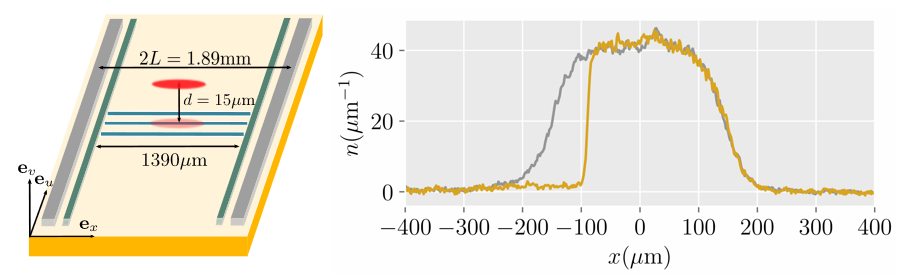
\includegraphics[width=0.90\linewidth]{Atom_chip.png}
\caption{(a) Schéma de la puce atomique. Les $3$ fils bleus assurent le confinement transverse, les $4$ autres fils (gris) génèrent le potentiel longitudinal. Le nuage atomique, représenté par une ellipse rouge, est piégé à $12~\mu$m au-dessus des fils. (b) Profils de densité linéique extraits par imagerie par absorption. En gris : gaz piégé dans un potentiel quartique. En jaune : après application du faisceau pousseur pendant $30~\mu$s, suivi d’un temps de vol de $1$~ms.}
\label{fig:setup}
\end{figure}

\section{Prédictions de la GHD}\label{sec.GHDpredictions}
\label{sec:ghd}

Le dispositif expérimental décrit ci-dessus peut être analysé théoriquement comme suit. Au cours de l'évolution temporelle, la frontière nette initiale du nuage devient plus lisse et les dérivées temporelles des quantités locales diminuent. Après un certain temps, après un lissage, on s'attend à ce que le gaz puisse être décrit localement par des états stationnaires.

Les états stationnaires du modèle de Lieb-Liniger sont complètement caractérisés par leur distribution de rapidité $\rho(\theta)$. Alternativement, ces états peuvent être caractérisés par le facteur d'occupation $\nu(\theta)$.% qui prend des valeurs entre 0 et 1, et qui est liée à la distribution de rapidité $\rho(\theta)$ par
%\begin{equation}
%\nu(\theta) = \frac{\rho(\theta)}{\rho_s(\theta)} \mbox{, \qquad où \qquad } \rho_s(\theta) =
%\frac{m}{2\pi \hbar} + \int \frac{d\theta'}{2\pi} \Delta(\theta-\theta') \rho(\theta') ,
%\end{equation}
%et $\Delta(\Theta) = \frac{2g}{\left(\frac{g^2}{\hbar} + \hbar \Theta^2\right)}$ est le "décalage de diffusion" dans le modèle de Lieb-Liniger. Les fonctions $\nu$ et $\rho$ sont en correspondance biunivoque, et dans ce qui suit, nous utilisons alternativement $\rho$ ou $\nu$. [Pour une introduction à ce formalisme, nous nous référons aux notes de cours \cite{doyon2020lecture} ou à la Section 1 de l'article de revue \cite{bouchoule_generalized_2022}.]

Puisque nous supposons une stationnarité locale, le système dans son ensemble est décrit par une distribution de rapidité dépendante du temps et de la position $\rho(x,\theta ; t )$, ou équivalemment par le facteur d'occupation dépendant du temps et de la position $\nu(x,\theta ; t)$. Ce dernier conduit à des calculs plus simples, tandis que le premier est particulièrement utile pour extraire la densité linéaire, qui est donnée par
\begin{equation}
    \label{eq:lineardensity}
	n(x;t) = \int d\theta \, \rho(x,\theta ; t ) .
\end{equation}

Les équations de GHD \cite{bertini_transport_2016,castro-alvaredo_emergent_2016} prédisent l'évolution temporelle de $\rho(x,\theta ; t)$, ou équivalemment de $\nu(x,\theta ; t)$. Lorsqu'elles sont écrites en termes du facteur d'occupation $\nu(x,\theta ; t )$, les équations de GHD prennent la forme d'une équation convective :
%\begin{subequations}
%\label{eq:GHD}
\begin{equation}
\label{eq:nu.cont}
\frac{\partial \nu}{\partial t} + v^{\rm{eff}}_{[\nu]} \frac{\partial \nu}{\partial x} = 0 ,
\end{equation}
et une deuxième relation qui fixe la vitesse effective $v^{\rm{eff}}_{[\nu]}$ comme une fonctionnelle de la distribution locale de rapidité (cf {??}).
%\begin{equation}
%v_{[\nu]}^{\rm{eff}}(\theta) = \theta - \int \Delta(\theta-\theta') \left( v^{\rm{eff}}_{[\nu]}(\theta) - v^{\rm{eff}}_{[\nu]}(\theta') \right) \rho(\theta') d\theta' .
%\end{equation}
%\end{subequations}
%Plus précisément, l'équation~(\ref{eq:GHD}a) est la forme à l'échelle d'Euler de la GHD, une équation sans diffusion valable aux grandes échelles. Des corrections diffuses, qui apparaissent sous forme d'un terme de type Navier-Stokes~\cite{de2018hydrodynamic,de2019diffusion,bastianello2020thermalization,de2022correlation}, ou même des corrections dispersives~\cite{de2023hydrodynamic}, ont également été étudiées théoriquement. Cependant, ces effets sont secondaires et n'ont pas été observés expérimentalement jusqu'à présent. Nous verrons plus bas que nos données expérimentales respectent le collage d'échelle attendu à l'échelle d'Euler (Fig.~\ref{fig:euler}), de sorte que ces effets semblent négligeables dans notre situation, du moins pour l'analyse des profils de frontière. Cela est également compatible avec une étude théorique récente dans le régime de faible interaction, qui a conclu que les effets diffusiques devraient être très faibles~\cite{moller2024identifying}. Par conséquent, dans cet article, nous ignorons la possibilité d'effets diffusiques secondaires (ainsi que tous les effets d'ordre supérieur) dans notre modélisation et nous nous en tenons à l'équation de GHD à l'échelle d'Euler ci-dessus.
\begin{figure}[!htb]
	\centering
	\includegraphics[width=\textwidth , page = 5 ]{Shema.pdf}
	\caption{
(a) À l'instant $t = 0^+$, immédiatement après le « quench bipartite » en $x = 0$, le facteur d'occupation est donné par $\nu(x, \theta ; t = 0^+) = \nu_0(\theta)$ pour $x > 0$ et est nul pour $x < 0$. Le bord initial représenté en tirets par l'ensemble des points $(x(s; t = 0^+) = 0,\ \theta(s; t = 0^+))$.
(b) Densité spatiale linéique $n(x)$ : en pointillés, $n(x; t = 0^-) = \int \rho(x, \theta; t = 0^-) \, \mathrm{d}\theta = n_0 = 56~\mu\mathrm{m}^{-1}$ juste avant le quench ; en ligne pleine, $n(x; t = 0^+) = n_0$ pour $x > 0$ et $0$ pour $x < 0$.
(c) À gauche de la coupure ($x < 0$) : en pointillés, $\nu(x, \theta ; t = 0^-) = \nu_0(\theta)$ ; en ligne pleine, $\nu(x, \theta ; t = 0^+) = 0$.
(d) À droite de la coupure ($x > 0$), le facteur d'occupation reste inchangé : $\nu(x, \theta ; t = 0^+) = \nu_0(\theta)$.
(e) À l'instant $t = 18~\mathrm{ms}$, après l'évolution balistique post-quench, le facteur d'occupation est donné par $\nu^\ast(x(s;t)/t, \theta) = \nu_0(\theta)$ pour $\theta < \theta(s;t)$, et nul pour $\theta > \theta(s;t)$, résolvant l'équation~(\ref{eq:nuetoile}), pour $t>0$. $\nu(x(s;t), \theta(s;t))(=\nu^\ast(x(s;t)/t, \theta(s;t)))$ est invarient de la déformation ie de $t>0$.  Le bord représenté en tirets par l'ensemble des points $(x(s; t)/t,\, \theta(s; t))$. Étant donné que la coupure initiale est en $x = 0$ et que l’évolution du bord est balistique, cette courbe résoud $v^{\mbox{\tiny eff}}_{[\nu^\ast(x(s; t)/t, \cdot) ]}(\theta(s; t)) = x(s; t)/t = v(s)$ (\ref{eq:nu.cont}).
(f) Densité spatiale réduite $n^\ast(x/t; t)$.
(g) Pour les atomes à droite de la coupure : en pointillés, $\nu^\ast(x(s;t)/t, \theta) = \nu_0(\theta)$ ; en ligne pleine, $\nu^\ast(x(s;t)/t, \theta) = \nu_0(\theta)$ pour $\theta < \theta(s;t)$ et nul pour $\theta > \theta(s;t)$. Le raisonnement est similaire pour les atomes à gauche de la coupure.
}
	\label{fig:BiPart.coupure1}
	
\end{figure}

%\begin{figure}[hbt]
%    \centering
    %\includegraphics[width=0.7\textwidth]{Figures/figure_nustar.pdf}
%    \caption{Facteur d'occupation $\nu^* (v,\theta)$ résolvant l'équation (\ref{eq:nuetoile}) pour un ratio d'occupation initial $\nu_0 (\theta)$ dans la moitié droite du système correspondant à un équilibre thermique à température $T$. La ligne verte pointillée est la courbe $\theta^*(v)$, c'est-à-dire l'ensemble des points $(v,\theta)$ tels que $v^{\rm eff}_{[\nu^* (v,\cdot)]} (\theta) = v$. [Paramètres : 
%    $\gamma_0=mg/(n_0\hbar^2)=0.005$, $k_B T \hbar^2/(mg^2) = 365$, proches des paramètres expérimentaux des jeux de données ci-dessous.]}
%    \label{fig:nu_star}
%\end{figure}

Pour une bipartition initiale dont la discontinuité est située à $x=0$, la solution de \eqref{eq:GHD} est invariante le long des rayons de vitesse constante $x/t$~\cite{bertini_transport_2016,castro-alvaredo_emergent_2016}. En d'autres termes, l'équation \eqref{eq:GHD} implique que, pour cette classe d'états initiaux, la distribution du facteur d'occupation local et donc toutes les propriétés locales du gaz, dépendent de $x$ et $t$ uniquement à travers la quantité $v=x/t$. La solution de l'équation \eqref{eq:GHD} peut donc être écrite en utilisant le facteur d'occupation le long des rayons $\nu^*(v,\theta)$ tel que
\begin{equation}
	\label{eq:nuvsnuetoile}
    \nu(x,t,\theta) = \nu^*( x/t,\theta).
\end{equation}

Pour la situation considérée dans cet article, où initialement un état de vide est situé pour $x < 0$ et un état de distribution du facteur d'occupation $\nu_0$ pour $x > 0$, la solution $\nu^*(v,\theta)$ est paramétrée par une rapidité de bord $\theta^*$ selon~\cite{bertini_transport_2016,castro-alvaredo_emergent_2016}
\begin{equation}
	\label{eq:nuetoile}
    \nu^*(v,\theta) = \left\{
    	\begin{array}{ccc}
    		\nu_0(\theta) & \text{si} & \theta < \theta^* \\
    		0 & \text{si} & \theta > \theta^* \\
   		\end{array}
    	\right. \quad \text{où} \quad  v^{\rm{eff}}_{[\nu^*(v,.)]}(\theta^*) = v.
\end{equation}
Cette équation peut être résolue numériquement pour toute distribution initiale donnée $\nu_0(\theta)$, voir la Fig.~\ref{fig:BiPart.coupure1} pour un exemple. Avec l'équation~\eqref{eq:nuvsnuetoile}, elle décrit entièrement le système à l'échelle d'Euler. Notez que, pour calculer la densité linéaire $n(x,t)$ afin de comparer avec les profils de densité expérimentaux, on utilise l'équation (\ref{eq:lineardensity}).

%\paragraph{Solution pour un système initialement dans l'état fondamental.}
%Pour illustrer le formalisme ci-dessus, explorons ses implications pour le cas spécial où la moitié droite du système est initialement dans l'état fondamental. Dans ce cas, le facteur d'occupation initial $\nu_0 (\theta)$ est une mer de Fermi : $\nu_0(\theta) = 1$ pour $|\theta| < \Delta\theta_0$, et $\nu_0(\theta) = 0$ sinon. Le rayon de Fermi $\Delta\theta_0$ dépend de la densité linéaire du gaz dans cette région, qui est constante. La distribution du facteur d'occupation se découpe ainsi en deux régions : pour $|\theta| > \Delta\theta_0$, $\nu_0(\theta) = 0$, et pour $|\theta| < \Delta\theta_0$, $\nu_0(\theta) = 1$. Au temps $t=0$, nous avons donc une discontinuité dans la distribution du facteur d'occupation à $\theta=\pm \Delta\theta_0$.

\section{Données expérimentales}\label{sec.ed}

L’état initial est préparé selon le protocole décrit en section~\ref{sub_pisih}. Le confinement longitudinal est ensuite supprimé, tandis que le confinement transverse est maintenu, afin d'étudier la dynamique le long de l’axe longitudinal.

Les profils de densité en bord obtenus pour des temps d’évolution compris entre $\tau = 10$~ms et $\tau = 18$ms sont présentés en Fig.\ref{fig:euler}(a), en fonction de la variable réduite $v = x/\tau$. L’excellent recouvrement des différents profils indique que l’échelle d’Euler est atteinte dans cet intervalle temporel. Au-delà de $\tau = 18$~ms, la dynamique longitudinale ne peut plus être explorée expérimentalement, en raison de la taille finie du gaz initial, préparé dans une configuration semi-homogène.

Pour des temps d’évolution plus courts, les profils de bord mesurés présentent une forme plus lissée que celle prédite par les équations de GHD à l’échelle d’Euler. Cette différence peut s’expliquer soit par une invalidité de l’approximation d’Euler dans ce régime transitoire, en lien avec de fortes variations de densité, soit par le fait que la coupure initiale à $t = 0$ n’est pas parfaitement abrupte, ce qui confère au bord initial une largeur finie.

\begin{figure}[!htb]
\centering
\includegraphics[width=1.0\linewidth]{DWD_GPE_vs_exp_V2.pdf}
\caption{(a) Profils de densité aux bords obtenus pour différents temps d’évolution $\tau$, représentés en fonction de $x/\tau$ ; (b) Comparaison du profil de bord mesuré avec la prédiction à température nulle issue de la GHD dans le régime quasi-condensat, donnée par l’équation~\eqref{eq:GPE}. Cette dernière constitue une excellente approximation pour la valeur du paramètre d’interaction correspondant aux données, soit $\gamma = 4{,}6 \times 10^{-3}$ (voir Fig.\ref{fig:boundary_profiles_theory}). Le profil de bord présenté en (b) est obtenu après un temps d’expansion de 10ms et provient d’un jeu de données différent de celui de la figure (a).}
\label{fig:euler}
\end{figure}

La figure~\ref{fig:euler}(b) présente une comparaison entre le profil de bord mesuré $n(v)$ et la prédiction théorique fondée sur un état initial à température nulle, supposé être l’état fondamental. Pour la valeur du paramètre de Lieb $\gamma = 4{,}6 \times 10^{-3}$, le profil est pratiquement indiscernable de celui obtenu dans le régime de quasi-condensat, justifiant l’utilisation de l’équation~\eqref{eq:GPE} pour la comparaison.

L’accord entre la prédiction théorique et les données expérimentales est satisfaisant, en particulier dans la région de forte densité. Les écarts observés par rapport à la forme parabolique prédite peuvent être attribués à des effets liés à une entropie non nulle, qui seront analysés dans la section suivante.

\section{Sonder la distribution locale des rapidités}
\label{sec:local}

Pour un état initial du gaz correspondant à un facteur d'occupation lisse $\nu(\theta)$ (par exemple un état thermique), le facteur d'occupation $\nu^*(x/t,\theta)$ à rapport $x/t$ fixé est attendu comme étant fortement asymétrique en fonction de $\theta$, selon l'équation~\eqref{eq:nuetoile}. En effet, du côté droite, il présente une discontinuité du type saut, similaire à celle du facteur d'occupation de l’état fondamental, tandis que du côté gauche, il reste lisse. Afin de révéler ces caractéristiques particulières de l’état local du gaz, nous utilisons le protocole introduit dans la Réf.~\cite{dubois_probing_2024} pour sonder la distribution locale des rapidités, comme expliqué ci-après.

Nous laissons d’abord le gaz se dilater pendant un temps $t=18~\mathrm{ms}$, de sorte que le bord s’étale sur une large zone d’environ $350~\mathrm{\mu m}$, comme illustré en Fig.~\ref{fig:BiPart.coupure1} (e)-(f) et  Fig ~\ref{fig:simul_deformation} (a).  
Nous sélectionnons ensuite une tranche du gaz comprise dans l’intervalle $[x_0-\ell/2, x_0+\ell/2]$, en éliminant tous les atomes situés hors de cette tranche à l’aide d’un faisceau de poussée~\cite{dubois_probing_2024}(Fig \ref{fig:BiPart.coupure2} (a)--(c)). 

\begin{figure}[!htb]
	\centering
	\includegraphics[width=\textwidth , page = 6 ]{Shema.pdf}
	\caption{
(a) À l'instant $\tau = 0^+$, immédiatement après la sélection de la tranche centrée en $x = x_0$ et de largeur $\ell$, la distribution de rapidité localement résolue est donnée par $\rho(x,\theta ; \tau = 0^+) = \nu(x, \theta ; t = 18~\mathrm{ms}) \, \rho_s(x,\theta ; t = 18~\mathrm{ms})$ pour $\vert x - x_0 \vert < \ell/2$, et est nulle pour $\vert x - x_0 \vert > \ell/2$. Le bord gauche immédiatement après la sélection est représenté en pointillés par l’ensemble des points $(x_g(s; \tau = 0^+),\ \theta_g(s; \tau = 0^+))$, et le bord droit en tiret-point par l’ensemble des points $(x_d(s; \tau = 0^+),\ \theta_d(s; \tau = 0^+))$. Le bord complet est donc la concaténation de ces deux ensembles. 
(b) Densité linéique spatiale $n(x)$ : en pointillés, $n(x; t = 18~\mathrm{ms})$ juste avant la sélection ; en ligne pleine, $n(x; \tau = 0^+)$, égal à $n(x; t = 18~\mathrm{ms})$ pour $\vert x - x_0 \vert < \ell/2$ et nul ailleurs. 
(c) Distribution de rapidité après sélection, $\Pi(\theta) = \int \rho(x,\theta ; \tau)\,\mathrm{d}x$, invariante sous l’évolution unidimensionnelle, représentée en rouge. La distribution localement résolue en $x(s; \tau = 0^+)$, $\rho(x(s; \tau = 0^+), \theta ; \tau = 0^+)$, est représentée en pointillés. Cette distribution est localement conservée, i.e., $\rho(x(s; \tau), \theta(s; \tau))$ reste inchangée au cours de l’évolution unidimensionnelle, indépendamment de $\tau$. 
(e) Distribution localement résolue $\rho(x, \theta ; \tau = 30~\mathrm{ms})$ après une évolution unidimensionnelle de $30~\mathrm{ms}$. Le bord gauche est représenté en pointillés par les points $(x_g(s; \tau = 30~\mathrm{ms}),\ \theta(s; \tau = 30~\mathrm{ms}))$, et le bord droit en tiret-point par $(x_d(s; \tau = 30~\mathrm{ms}),\ \theta(s; \tau = 30~\mathrm{ms}))$. 
(f) Densité spatiale réduite $n(x; \tau = 30~\mathrm{ms})$. 
(g) Distribution de rapidité $\Pi(\theta)$ après la sélection (identique à celle de (c)).
}
	\label{fig:BiPart.coupure2}
	
\end{figure}
 
En Fig.~\ref{fig:simul_deformation}(a), nous présentons le profil de densité mesuré $1$ ms après la sélection de la tranche.  
L’ajustement à une fonction rectangulaire lissée donne $x_0 = 18\,\mu$m.  
Pour les calculs, la largeur $\ell$ sera déterminée à partir du nombre d’atomes sélectionnés (voir ci-dessous).  
Enfin, nous laissons cette tranche se dilater en 1D pendant un temps d’expansion $\tau$, puis nous mesurons la densité longitudinale $\tilde{n}(x,\tau)$.  
Celle-ci reflète la distribution totale des rapidités dans la tranche $\Pi(\theta) = \int \rho(x, \theta ; \tau > 0)\, dx = \int_{x_0 - \ell/2}^{x_0 + \ell/2} \rho(x, \theta ; \tau = 0^+)\, dx$, car pour $\tau \rightarrow \infty$, on s’attend à ce que $\tau \tilde{n}( \tau * \theta - x_0  ;\tau) \simeq \Pi(\theta)$.  
L’asymétrie attendue de $\Pi$ devrait ainsi induire une asymétrie de la densité $\tilde{n}(x,\tau)$ en fonction de $x$.  
Nous observons effectivement cette asymétrie dans nos profils d’expansion, comme illustré en Fig.~\ref{fig:simul_deformation}(b) pour un temps d’expansion $\tau=30$ ms.

\begin{figure}[!htb]
\centering
\begin{tikzpicture}
    \node[rectangle, draw = none] (bord) at (0,0) {
        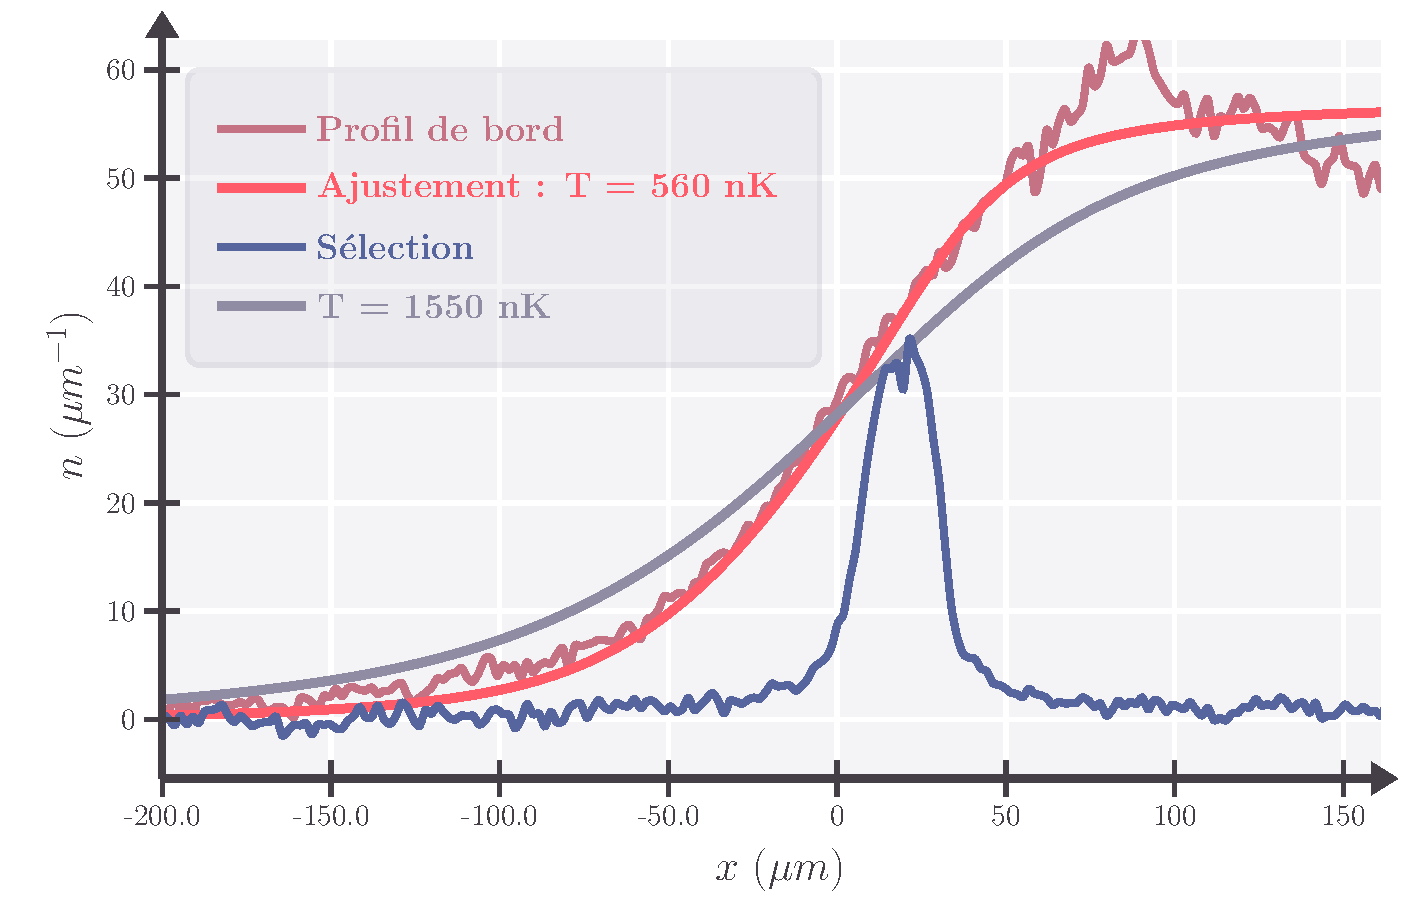
\includegraphics[width=0.5\textwidth , page = 1]{Figures}
    };
    \node[circle, draw=none, above=0cm of bord , shift={( -2.5cm , -0.5cm )} ] {(a)};
    
    \node[right=1mm of bord , shift={( -0.5cm , 0cm )}] (assy) {
        \includegraphics[width=0.5\textwidth , page = 2 ]{Figures}
    };
    \node[circle, draw=none, above=0cm of assy , shift={( -2.5cm , -0.5cm )}] {(b)};
\end{tikzpicture}
\caption{(a) {\it Profil de bord et tranche sélectionnée.} Le profil de bord après $18\,\mathrm{ms}$ est montré en rouge. L'ajustement thermique donne une température $T = 560\,\mathrm{nK}$ (orange). Le profil de densité mesuré $1\,\mathrm{ms}$ après la sélection de la tranche est en bleu. (b) {\it Asymétrie du profil d’expansion de la tranche.} Le profil de densité après une expansion pendant $\tau = 30\,\mathrm{ms}$ est comparé à son image miroir. Le centre de symétrie $x_s = -17\,\mu$m minimise la distance quadratique $\delta^2 = \int dx\, (\tilde{n}(x) - \tilde{n}(2x_s - x))^2$.}
\label{fig:simul_deformation}
\end{figure}

Pour aller au-delà de cette observation qualitative, nous effectuons un calcul GHD à l’échelle d’Euler du profil d’expansion, en supposant que l’état initial est thermique.  
La température est obtenue par ajustement du profil de bord avant la sélection de la tranche, comme indiqué en Fig.~\ref{fig:simul_deformation}(a), ce qui donne $T = 560$ nK.  
Le potentiel chimique est ajusté afin que la densité linéaire initiale corresponde à celle mesurée dans la région $x > 0$, avant l’élargissement du bord.  
À partir du profil initial, nous simulons à la fois l’élargissement du bord et l’expansion de la tranche en GHD, en supposant une découpe parfaite, c’est-à-dire $\nu(x,\theta) = 0$ pour $|x - x_0| > \ell/2$ et $\nu(x,\theta)$ inchangé sinon.  
La largeur $\ell$ est ajustée de sorte que le nombre d’atomes sélectionnés dans la simulation corresponde à celui mesuré expérimentalement après expansion, et on obtient $\ell = 24\,\mu$m.  

Le profil d’expansion simulé est montré en Fig.~\ref{fig:simul_expansion}(a).  
Il présente une forte asymétrie, comme attendu, avec un bord droit abrupt et une densité nulle au-delà d’un certain point.  
Cependant, cette chute est moins marquée que celle prédite pour la distribution locale des rapidités $\rho(x_0,\theta)$ à $x = x_0$. Deux effets contribuent à cet élargissement :  
(i) la distribution en rapidité n’est pas homogène à l’intérieur de la tranche, si bien que $\Pi(\theta)$ diffère de $\ell \rho(x_0,\theta)$, comme le montre la comparaison entre la ligne marron pleine et la ligne pointillée en Fig.~\ref{fig:simul_expansion}(a) ;  
(ii) le temps d’expansion est fini, de sorte que le profil observé $\tilde{n}(x, {\tau} )$ ne correspond pas exactement à $\Pi((x-x_0)/\tau)/\tau$, comme le montre la comparaison entre les courbes marron et rouge.



%l'ensemble $\{(x_g(1; \tau = 0^+) ,\ \theta(1; \tau = 0^+)) , \cdots , (x_g(q; \tau = 0^+) ,\ \theta(q; \tau = 0^+)) , (x_d(1; \tau = 0^+) ,\ \theta(1; \tau = 0^+)) , \cdots , (x_d(q; \tau = 0^+) ,\ \theta(q; \tau = 0^+)) \}$ ou $q$ est la taille des deux ensemble.



\begin{figure}[!htb]
\centering
\begin{tikzpicture}
    \node[rectangle, draw = none] (exp) at (0,0) {
       \includegraphics[width=0.5\textwidth , page = 3]{Figures}
    };
    \node[circle, draw=none, above=0cm of exp , shift={( -2.5cm , -0.5cm )} ] {(a)};
    
    \node[right=1mm of exp , shift={( -0.5cm , 0cm )}] (pi) {
       \includegraphics[width=0.5\textwidth , page = 4]{Figures}
    };
    \node[circle, draw=none, above=0cm of pi , shift={( -2.5cm , -0.5cm )}] {(b)};
\end{tikzpicture}
\caption{(a) {\it Profil de densité après expansion de la tranche : effets de la largeur finie et du temps d’expansion fini.} Courbe orange : profil obtenu par simulation GHD après expansion pendant $\tau = 30$ ms, avec $T = 560$ nK. Courbe marron : distribution asymptotique $\Pi((x - x_0)/\tau)/\tau$. Courbe pointillée noire : approximation $\ell \rho(x_0, (x - x_0)/\tau)/\tau$ dans le cas d’une tranche étroite. (b) {\it Comparaison aux données expérimentales.} En bleu : profil expérimental après expansion pendant $\tau = 30$ ms. En orange : simulation GHD avec $T = 560$ nK. En magenta : ajustement du profil expérimental donnant $T = 1550$ nK.}
\label{fig:simul_expansion}
\end{figure}

Nous comparons ensuite le profil d'expansion simulé par la GHD avec les données expérimentales. Comme montré en Fig.~\ref{fig:simul_expansion}(b), le profil prédit reproduit les principales caractéristiques du profil d'expansion observé expérimentalement. Des écarts atteignant 25\,\% sont cependant visibles dans la partie centrale du profil. Afin d'obtenir un meilleur accord entre données et calculs, nous avons ajusté le profil d'expansion expérimental avec le calcul GHD en utilisant la température de l'état initial comme paramètre d'ajustement. Le résultat, représenté par la ligne magenta dans la Fig.~\ref{fig:simul_expansion}(b), donne une température $T=1550$~nK, plus de deux fois supérieure à celle obtenue en ajustant le profil au bord. Le profil au bord calculé pour cette température n'est pas compatible avec le profil expérimental, comme le montre la Fig.~\ref{fig:simul_expansion}(b).

Une des raisons de l'échec de nos tentatives de reproduction du profil de densité après l'expansion de la tranche réside dans la présence de queues à droite du profil expérimental — voir le profil de densité dans la Fig.~\ref{fig:simul_expansion}(b). Ces queues sont absentes des calculs GHD à l’échelle d’Euler car la fonction d’occupation dans la tranche s’annule strictement au-delà d’une certaine rapidité. L’origine de ces queues reste incertaine. Elles pourraient être dues à des effets de bord associés à la procédure de sélection de tranche, les atomes en bordure étant chauffés par le faisceau de poussée. Il est également possible qu’un effet diffusif, non pris en compte dans la GHD à l’échelle d’Euler, intervienne au début de la déformation du bord, lorsque les gradients sont importants.

\section{Détails sur les calculs}
\label{sec:calcule}

On fait l'hypothèse que le système est dans un état thermique. Cela implique que la fonction $w$ qui paramétrise l'opérateur charge (cf. ??) vérifie :

\begin{eqnarray*}
	w(\theta) & = &  \beta(\varepsilon(\theta) - \mu),
\end{eqnarray*}

avec $\beta = (k_B T)^{-1}$ et $\varepsilon(\theta) = \frac{m \theta^2}{2}$. On peut réécrire cette relation en minimisant l'entropie de Yang-Yang (cf. ??) et en injectant la forme du facteur d'occupation $\nu = \rho/\rho_s = (1+e^{\beta \epsilon})^{-1}$ . On obtient alors une équation de type point fixe :

\begin{eqnarray*}
	\beta \epsilon & = & \beta \epsilon_0 -  \frac{\Delta}{2\pi} \star \ln \left( 1 + e^{-\beta \epsilon} \right) ,
\end{eqnarray*}

avec $\epsilon_0 = \varepsilon - \mu$. Cette équation est bien définie et converge (cf. ??). Pour s'en convaincre, on peut calculer la norme du déterminant du jacobien de l'application. Si elle est inférieure à 1, on est assuré de la convergence. 

L'équation étant non linéaire, pour garantir la convergence vers la bonne solution (évitant les cycles), on itère la suite suivante :

\begin{eqnarray*}
	\beta \epsilon_{n+1} & = & \beta \epsilon_0 -   \frac{\Delta}{2\pi} \star \ln \left( 1 + e^{-\beta \epsilon_n} \right) ,
\end{eqnarray*}

jusqu'à ce que la distance entre deux itérations successives soit suffisamment petite : ici $\beta \Vert \epsilon_{n+1} - \epsilon_n \Vert < 10^{-12}$.

Ainsi, en fixant le couple $(\mu, T)$, on obtient $\epsilon$, puis $\nu$, puis enfin $\rho_s$ via :

\begin{eqnarray*}
	2\pi \rho_s & = & \frac{m}{\hbar} \ast 1^{\mathrm{dr}},
\end{eqnarray*}

où la fonction "habillée" $f^{\mathrm{dr}}$ est définie par :

\begin{eqnarray*}
	f^{\mathrm{dr}} & = & f + \frac{\Delta}{2\pi} \star ( \nu \ast f^{\mathrm{dr}} ),
\end{eqnarray*}

ce qui est une équation linéaire. Numériquement, on la résout sous la forme :

\begin{eqnarray*}
	\left\{ \mathrm{id} - \frac{\Delta}{2\pi} \star ( \nu \ast \cdot ) \right\} f^{\mathrm{dr}} & = & f.
\end{eqnarray*}

La densité physique est alors obtenue par $\rho = \nu \ast \rho_s$. Expérimentalement, on mesure la densité homogène $n_0 = 56~\mathrm{\mu m^{-1}}$ (voir Fig. \ref{fig:BiPart.insitut}). À température fixée, on ajuste donc le potentiel chimique $\mu$ pour satisfaire la contrainte :

\begin{eqnarray*}
	n_0 & = & \int \rho(\theta) \, d\theta.
\end{eqnarray*}

L'équation (\ref{eq:nuetoile}) implique :

\begin{eqnarray*}
	\nu(x(s;t), \theta(s;t)) & = & \nu(x(s;0), \theta(s;0)),
\end{eqnarray*}

ce qui signifie que $\nu$ est constant au cours du temps si on suit le couple $(x(s;t), \theta(s;t))$ — c’est la vision lagrangienne en hydrodynamique. La graduation fixe des axes donne la vision eulérienne. Cela implique également :

\begin{eqnarray*}
	\partial_t \left( \begin{array}{c} x(s;t) \\ \theta(s;t) \end{array} \right) & = & \left( \begin{array}{c} v^{\mathrm{eff}}_{[\nu]}(\theta(s;t)) \\ 0 \end{array} \right),
\end{eqnarray*}

d’où $\theta(s;t) = \theta(s;0) \equiv \theta(s)$. On note $\Gamma_t \doteq \{(x(s;t), \theta(s;t))\}$. À l’intérieur de ce contour, le facteur d’occupation est indépendant de $x$ (voir Fig. ??), donc il est conservé au cours du temps :

\begin{eqnarray*}
	\nu(x(s,t), \theta(s)) & = & \nu_0(\theta),
\end{eqnarray*}

ce qui est le cas dans tout le protocole. On peut ainsi calculer l’évolution du contour au cours du temps.


\subsection{Simulation de la déformation du bord} 

Dans la partie "déformation du bord" (Fig. \ref{fig:BiPart.coupure1}), initialement, l'intérieur du contour correspond à $x > 0$. Il est donc suffisant d'étudier l'évolution du bord initialement situé en $(x(s, t = 0 ) = 0 , \theta(s))$. La bijectivité du contour implique que la vitesse effective soit constante : $v_{[\nu]}^{\mbox{\tiny eff}} ( \theta  ) = v$, d'où

\begin{eqnarray*}
	\frac{x(s;t)}{t} & = &	v_{[\nu^\ast (  v(s) , \cdot )]}^{\mbox{\tiny eff}} ( \theta(s)  ) = v(s),
\end{eqnarray*}

avec la mise à l’échelle suivante :

\begin{eqnarray*}
	\nu(x(s,t),\theta(s)) & = &  \nu^\ast(v(s),\theta(s)),
\end{eqnarray*}

ce qui montre que la déformation est indépendante du temps. Ainsi, pour simuler la déformation du bord, il suffit de calculer la vitesse effective :

\begin{eqnarray*}
	v_{[\nu]}^{\mbox{\tiny eff}} ( \theta  ) & = & \frac{\mathrm{id}^{\mathrm{dr}}(\theta)}{\mathrm{1}^{\mathrm{dr}}(\theta)}.
\end{eqnarray*}

Une fois cette vitesse obtenue, on peut en déduire la position du bord après un temps $t$ de déformation :

\begin{eqnarray*}
	x(s;t) & = & v_{[\nu]}^{\mbox{\tiny eff}} ( \theta  ) \cdot t.	
\end{eqnarray*}

Connaissant le bord au temps $t$, on en déduit le facteur d’occupation (Fig. \ref{fig:BiPart.coupure1}(e)(g)), et donc la densité linéique $n(x,t)$ (Fig. \ref{fig:BiPart.coupure1}(e)(f)).

Sachant que $n_0 = 56~\mathrm{\mu m}^{-1}$ et que $\mu$ dépend de $T$ et de $n_0$, on ajuste la température des simulations GHD sur les données expérimentales de la déformation du bord (Fig. \ref{fig:simul_deformation}). Cet ajustement donne $T = 560~\mathrm{nK}$.

\subsection{Simulation de l’expansion}

Nous effectuons une sélection du système après la déformation du bord (Fig. \ref{fig:BiPart.coupure2}(a)) et nous procédons à une expansion unidimensionnelle de cette tranche (Fig. \ref{fig:BiPart.coupure2}(e)). Contrairement au cas de la déformation du bord, le contour n’est ici pas bijectif. La vitesse effective $v^{\mathrm{eff}}_{[\nu(x(s;\tau),\cdot)]}(\theta(s))$ dépend donc du temps d’expansion $\tau$.

Pour contourner cela, nous découpons le contour en deux parties : le bord gauche $(x_g(s, t), \theta_g(s))$ et le bord droit $(x_d(s, t), \theta_d(s))$, de sorte que ces deux bords soient bijectifs (Fig. \ref{fig:BiPart.coupure2}(a) et (e)). Avec cette découpe, après une expansion unidimensionnelle d’une durée $\tau$, le facteur d’occupation devient :

\begin{eqnarray*}
	\nu ( x(s;\tau), \theta ) & = & 
	\left\{ 
	\begin{array}{rcl}
	\nu_0(\theta) & \mbox{si} & \theta \in [\theta_g(s), \theta_d(s)] \\
	0 & \mbox{sinon} & 
	\end{array} 
	\right.
\end{eqnarray*}

Ayant la connaissance de $v^{\mathrm{eff}}_{[\nu(x(s;\tau),\cdot)]}(\theta(s))$, on peut suivre l’évolution du contour, et donc de la densité spatiale $n(x,t)$ (Fig. \ref{fig:BiPart.coupure2}(f)). 

Après avoir réalisé une simulation GHD avec $T = 560~\mathrm{nK}$, valeur obtenue via l’ajustement sur la déformation du bord, on compare cette simulation aux données expérimentales après $\tau = 30~\mathrm{ms}$ d’expansion. On compare alors la courbe orange aux données en bleu dans la Fig. \ref{fig:simul_expansion}(b). 

La simulation ne reproduit pas bien les données, comme attendu : certains phénomènes physiques ne sont pas pris en compte dans les simulations GHD. Cela se manifeste notamment autour de $\pm 350~\mu\mathrm{m}$. 

Nous avons donc effectué un ajustement direct de $T$ sur les données après expansion (courbe grise de la Fig. \ref{fig:simul_expansion}(b)).

 







\chapter{Mise en place d'un confinement longitudinale dipolaire}
\minitoc
\section{calculs}
\section{laser , MOPA, etc .. Données}

\appendix

\chapter{Calcules Hamiltonien à N fixés}
\section{deux particules}\label{annex:2.part}
%\subsubsection{Polarisation linéaire  et $d_0 \equiv \langle nP , m_L = 0 \vert \operatorvec{D} \cdot \operatorvec{u} \vert nS , m_L = 0 \rangle $}
\subsubsection{Polarisation linéaire}

On se limide à une polarisation laser linéaire. Par consequence dans la base $\vert  n , L , m_L \rangle$, il y a uniquement la transition $\vert n S , m_L = 0 \rangle \equiv \vert n , L = 0 , m_L = 0 \rangle \to \vert n P , m_L = 0 \rangle \equiv \vert n , L = 1 , m_L = 0 \rangle $.
Pour la suite on note %$d_0 \equiv \langle nP , m_L = 0 \vert \operatorvec{D} \cdot \operatorvec{u} \vert nS , m_L = 0 \rangle$ 
\begin{eqnarray*}
	d_0 & \equiv & \langle nP , m_L = 0 \vert \operatorvec{D} \cdot \operatorvec{u} \vert nS , m_L = 0 \rangle.	
\end{eqnarray*}


%\subsubsection{Dans la base fine et $ \langle n{~}^2P_{1/2} , m_J = 1/2 \vert \operatorvec{D} \cdot \operatorvec{u} \vert n{~}^2S_{1/2} , m_J = 1/2 \rangle = d_0 / \sqrt{3}$}
\subsubsection{Dans la base fine}

Le moment angulaire électronique total , $J = S + L$ , est la somme du nombre quantique de moment angulaire totale $L$ et du spin totale des électrons. Ici on ne considère juste la couche de valence et on se limete au alcalin donc $S = 1/2 $.\\

Décomposons $\vert n{~}^2P_{3/2} , m_J = 1/2 \rangle \equiv \vert n , J = 3/2 , m_J = 1/2 \rangle $ dans la base  $  \vert n , m_S  , m_L \rangle  \equiv \vert  n{~}^2P , m_S  ,  m_L \rangle \equiv \vert n  , S=1/2 , m_S , L=1 , m_L \rangle $.\\
On sait que 
\begin{eqnarray}
	\vert n , J = {3}/{2} , m_J = {3}/{2} \rangle & = &  \vert n , m_S = 1/2   , m_L = 1 \rangle
\end{eqnarray}
or
\begin{eqnarray}
	\operator{A}_\pm \vert n , A , m	_A \rangle & = & \hbar \sqrt{A(A+1) - m_A(m_A\pm 1 ) } \vert n , A , m	_A \pm 1  \rangle
\end{eqnarray}

avec l'opérateur $\operator{A} \in \{ \operator{S} , \operator{L} , \operator{J} , \cdots \}$. Donc  

\begin{eqnarray}
	\operator{J}_- \vert n , J = 3/2  , m_J = 3/2 \rangle & = & \hbar \sqrt{\frac{3}{2}\left(\frac{5}{2} \right ) - \frac{3}{2}\left(\frac{1}{2} \right )  } \vert n , J = 3/2  , m_J = 1/2  \rangle, \notag \\
	& = & \hbar \sqrt{3} \vert n , J = 3/2  , m_J = 1/2  \rangle.
\end{eqnarray}

or 

\begin{eqnarray}
	\operator{J}_- & = & 	\operator{S}_- + \operator{L}_-	
\end{eqnarray}

\begin{eqnarray}
	\operator{J}_- \vert n , J = 3/2  , m_J = 3/2 \rangle & = & (\operator{S}_- + \operator{L}_-) \vert n , m_S = 1/2   , m_L = 1 \rangle,\\
	& = & \hbar \sqrt{\frac{1}{2}\left(\frac{3}{2} \right ) - \frac{1}{2}\left(-\frac{1}{2} \right ) }	\vert n , m_S = -1/2   , m_L = 1 \rangle \notag \\
	& + & \hbar \sqrt{1\left(2 \right ) - 1\left(0\right ) }	\vert n , m_S = 1/2   , m_L = 0 \rangle \notag \\
	& = & \hbar \vert n , m_S = -1/2   , m_L = 1 \rangle \\ & + & \hbar \sqrt{2}	\vert n , m_S = 1/2   , m_L = 0 \rangle  
\end{eqnarray}

Donc d'après les équations ???

\begin{eqnarray}
	\vert nP_{3/2}  , m_J = 1/2  \rangle & = & \frac{1}{\sqrt{3} } \vert n , m_S=-1/2  , m_L=1 \rangle + \sqrt{\frac{2}{3}} \vert n , m_S=1/2  , m_L=0 \rangle			
\end{eqnarray}

avec $\vert nP_J  , m_J   \rangle \equiv \vert n , J  , m_J  \rangle$ et $\vert n , m_S  , m_L \rangle	 \equiv \vert n   , S=1/2 , m_S , L=1 , m_L \rangle = \vert n {~}^2P  , m_S , m_L \rangle $.\\

Pour aussi 
\begin{eqnarray}
	\vert nP_{1/2}  , m_J = 1/2   \rangle  & \in & 	\bm{Vect} \{ \vert n , m_S = -1/2  , m_L = 1  \rangle , \vert n , m_S = 1/2  , m_L = 0  \rangle  \} ,\\
	\langle  nP_{3/2}  , m_J = 1/2 \vert nP_{1/2}  , m_J = 1/2   \rangle & = & 0 		
\end{eqnarray}
Donc 

\begin{eqnarray}
	\vert nP_{1/2}  , m_J = 1/2  \rangle & = & \mp \sqrt{\frac{2}{3}} \vert n , m_S=-1/2  , m_L=1 \rangle \pm \frac{1}{\sqrt{3} }   \vert n , m_S=1/2  , m_L=0 \rangle		
\end{eqnarray}

et 
\begin{eqnarray}
	\vert nP_{1/2}  , m_J = -1/2   \rangle  & \in & 	\mathrm{Vect} \{ \vert n , m_S = 1/2  , m_L = -1  \rangle , \vert n , m_S = -1/2  , m_L = -0  \rangle  \} ,\\
	\vert nP_{3/2}  , m_J = -3/2   \rangle & = & \vert n , m_S = -1/2  , m_L = -1  \rangle		
\end{eqnarray}


et 

\begin{eqnarray}
	\hbar \sqrt{3} \vert n , J = 3/2  , m_J = -1/2 \rangle & \leftrightharpoons & \notag \\
	\hbar {\textstyle \sqrt{\frac{3}{2} \left ( \frac{5}2 \right ) -  \left ( -\frac{3}{2} \right ) \left ( -\frac{1}{2} \right )}} \vert n , J = 3/2  , m_J = -1/2 \rangle & \leftrightharpoons & \notag \\
	\operator{J}_+ \vert n , J = 3/2  , m_J = -3/2 \rangle & \leftrightharpoons & \notag \\
	\operator{J}_+ \vert n {~}^2P_{3/2}  , m_J = -3/2 \rangle & = & (\operator{S}_+ + \operator{L}_+)	\vert n {~}^2 P , m_S = -1/2  , m_L = -1  \rangle, \notag\\
	& \rightleftharpoons &	(\operator{S}_+ + \operator{L}_+)	\vert n , m_S = -1/2  , m_L = -1  \rangle, \notag\\
	& \rightleftharpoons &	\hbar 	{\textstyle \sqrt{\frac{1}{2} \left ( \frac{3}2 \right ) -  \left ( -\frac{1}{2} \right ) \left ( \frac{1}{2} \right )}}\vert n , m_S = 1/2  , m_L = -1  \rangle, \notag\\
	& + & \hbar 	{\textstyle \sqrt{1 \left ( 2 \right ) -  \left ( -1 \right ) \left ( 0 \right )}}\vert n , m_S = -1/2  , m_L = 0  \rangle, \notag\\
	& \rightleftharpoons & \hbar \vert n , m_S = 1/2  , m_L = -1  \rangle \notag \\
	& + & \hbar \sqrt{2}\vert n , m_S = -1/2  , m_L = 0  \rangle \notag 
\end{eqnarray}

soit 

\begin{eqnarray}
	\vert n {~}^2P_{3/2}  , m_J = -1/2 \rangle	 & = & 	 \sqrt{\frac{1}{3} }\vert n {~}^2P  , m_S = 1/2  , m_L = -1 \rangle + \sqrt{\frac{2}{3} }\vert n {~}^2P  , m_S =-1/2  , m_L = 0 \rangle \notag
\end{eqnarray}

Or 

\begin{eqnarray}
	\vert n {~}^2P_{1/2}  , m_J = -1/2 \rangle & \in & \mathrm{Vect}	 \{ \vert n {~}^2P  , m_S = 1/2  , m_L = -1 \rangle , \vert n {~}^2P  , m_S = -1/2  , m_L = 0 \rangle \} \notag,\\
	\langle n {~}^2 P_{3/2} , m_J = -1/2 \vert n {~}^2P_{1/2}  , m_J = -1/2 \rangle & = & 0 \notag 			
\end{eqnarray}

Soit 

\begin{eqnarray}
	\vert n {~}^2P_{1/2}  , m_J = -1/2 \rangle & = & \mp \sqrt{ \frac{2}{3}} \vert n {~}^2P  , m_S = 1/2  , m_L = -1 \rangle \pm  \sqrt{ \frac{1}{3}} \vert n {~}^2P  , m_S = -1/2  , m_L = 0 \rangle  \notag,		
\end{eqnarray}

\begin{eqnarray}
	\vert n {~}^2S_{1/2} , m_J = \pm 1/2 \rangle & = & 	\vert n {~}^2S , m_S = \pm 1/2 , m_L = 0 \rangle  \equiv  \vert n {~}^2S , m_S = \pm 1/2  \rangle , \notag \\
	\vert n {~}^2P_{1/2}  , m_J = \pm 1/2 \rangle & = & \epsilon \sqrt{ \frac{2}{3}} \vert n {~}^2P  , m_S = \mp 1/2  , m_L = \pm 1 \rangle -\epsilon  \sqrt{ \frac{1}{3}} \vert n {~}^2P  , m_S = \pm 1/2  , m_L = 0 \rangle  \notag,	\\
	\vert n {~}^2P_{3/2}  , m_J = \pm 1/2 \rangle & = & + \sqrt{ \frac{1}{3}} \vert n {~}^2P  , m_S = \mp 1/2  , m_L = \pm 1 \rangle +  \sqrt{ \frac{2}{3}} \vert n {~}^2P  , m_S = \pm 1/2  , m_L = 0 \rangle  \notag,	\\
	\vert n {~}^2P_{3/2} , m_J = \pm 3/2 \rangle & = & 	\vert n {~}^2P , m_S = \pm 1/2 , m_L = \pm 1  \rangle , \notag 
\end{eqnarray}

avec $\epsilon \in \{ +1 , -1 \} $.\\

\begin{aligned} \ket{n\,^2P_{1/2},+\tfrac12} &= -\sqrt{\tfrac{1}{3}}\,\ket{m_L=0,\,m_S=+\tfrac12} \;+\;\sqrt{\tfrac{2}{3}}\,\ket{m_L=+1,\,m_S=-\tfrac12},\\ \ket{n\,^2P_{1/2},-\tfrac12} &= +\sqrt{\tfrac{1}{3}}\,\ket{m_L=0,\,m_S=-\tfrac12} \;-\;\sqrt{\tfrac{2}{3}}\,\ket{m_L=-1,\,m_S=+\tfrac12}. \end{aligned}

\begin{aligned} \ket{n\,^2P_{3/2},+\tfrac12} &= +\sqrt{\tfrac{2}{3}}\,\ket{m_L=0,\,m_S=+\tfrac12} \;+\;\sqrt{\tfrac{1}{3}}\,\ket{m_L=+1,\,m_S=-\tfrac12},\\ \ket{n\,^2P_{3/2},-\tfrac12} &= +\sqrt{\tfrac{2}{3}}\,\ket{m_L=0,\,m_S=-\tfrac12} \;+\;\sqrt{\tfrac{1}{3}}\,\ket{m_L=-1,\,m_S=+\tfrac12}. \end{aligned}


Si la polarisation de la lumière est linéaire, cela signifie que les oscillations des champs électriques et magnétiques se produisent dans un seul plan. Dans ce cas, l'opérateur dipôle électronique $\operatorvec{D} \cdot \operatorvec{u}$ n'affectera pas directement les nombres quantiques magnétiques $m_L$ ou $m_J$, car la polarisation linéaire ne change pas l'orientation du moment angulaire ou du spin $m_S$ de la particule. 



\begin{eqnarray*}
	\langle n {~}^2P_{1/2} , m_J = \pm  1/2 \vert \operatorvec{D} \cdot \operatorvec{u}\vert n {~}^2S_{1/2} , m_J = \pm  1/2 \rangle	& & =  \\  \epsilon \sqrt{\frac{2}{3}} \underbrace{\langle n {~}^2P , m_S = \mp  1/2  , m_L = \pm 1 \vert \operatorvec{D} \cdot \operatorvec{u}\vert n {~}^2S , m_S = \pm  1/2 , m_L = 0  \rangle}_{0}  & + & \\
	- \epsilon  \sqrt{\frac{1}{3}}\underbrace{\langle n {~}^2P , m_S = \pm  1/2  , m_L = 0 \vert \operatorvec{D} \cdot \operatorvec{u}\vert n {~}^2S , m_S = \pm  1/2 , m_L = 0  \rangle	}_{d_0},\\
	\langle n {~}^2P_{1/2} , m_J = \pm  1/2 \vert \operatorvec{D} \cdot \operatorvec{u}\vert n {~}^2S_{1/2} , m_J = \pm  1/2 \rangle	 &=& - \epsilon \sqrt{\frac{1}{3}} d_0
\end{eqnarray*}

\begin{eqnarray*}
	\langle n {~}^2P_{3/2} , m_J = \pm  1/2 \vert \operatorvec{D} \cdot \operatorvec{u}\vert n {~}^2S_{1/2} , m_J = \pm  1/2 \rangle	& & =  \\  \sqrt{\frac{1}{3}} \underbrace{\langle n {~}^2P , m_S = \pm  1/2  , m_L = \mp 1 \vert \operatorvec{D} \cdot \operatorvec{u}\vert n {~}^2S , m_S = \pm  1/2 , m_L = 0  \rangle}_{0}  & + & \\
	 \sqrt{\frac{2}{3}}\underbrace{\langle n {~}^2P , m_S = \pm  1/2  , m_L = 0 \vert \operatorvec{D} \cdot \operatorvec{u}\vert n {~}^2S , m_S = \pm  1/2 , m_L = 0  \rangle	}_{d_0},\\
	\langle n {~}^2P_{3/2} , m_J = \pm  1/2 \vert \operatorvec{D} \cdot \operatorvec{u}\vert n {~}^2S_{1/2} , m_J = \pm  1/2 \rangle	 &=& \sqrt{\frac{2}{3}} d_0
\end{eqnarray*}

\subsubsection{Potentiel dipolaire}

En négligeant le temps non-resonant et avec l'hipothèse $\vert \omega_b - \omega_a -\omega  \vert \gg \gamma_{ab} $ ( $V_{AR} = \delta E$) l'équation ???? devient :

\begin{eqnarray*}
	V_{AR} & = & - \frac{ \vert \mathcal{E} \vert^2}{4 \hbar} \left( \frac{ \vert \langle n {~}^2P_{1/2}  \vert \operatorvec{D} \cdot \operatorvec{u}\vert n {~}^2S_{1/2}  \rangle \vert^2}{ \Delta_1} + \frac{ \vert\langle n {~}^2P_{3/2}  \vert \operatorvec{D} \cdot \operatorvec{u}\vert n {~}^2S_{1/2}  \rangle \vert^2}{ \Delta_2}  \right ) , \\
	&  = &  - \frac{  d_0^2 \vert \mathcal{E} \vert^2 }{4 \hbar} \left( \frac{ 1}{ 3 \Delta_1} + \frac{2 }{ 3 \Delta_2}  \right ) ,		
\end{eqnarray*}
avec $\Delta_i = \omega_i - \omega $ avec $ i \in \{ 1 , 2 \}$ avec $\omega_1 = \omega_{n {~}^2P_{1/2}, m_J = \pm  1/2}- \omega_{n {~}^2S_{1/2}, m_J = \pm  1/2}$ et $\omega_2 = \omega_{n {~}^2P_{3/2}, m_J = \pm  1/2} - \omega_{n {~}^2S_{1/2}, m_J = \pm  1/2}$

\subsubsection{Relier Intensité laser et $\mathcal{E}$}

La densité d'énergie électromagnétique:

\begin{eqnarray}
	u_{em} & = &  \frac{1}2 \left ( \varepsilon_0  \Re ( \vec{E} ) ^2 + \frac{1}{\mu_0} \Re(\vec{B})^2 \right ) \\
	\langle u_{em} \rangle & =& \frac{\varepsilon_0 \langle \Re(\vec{E})^2 \rangle}{2} + \frac{\langle \Re(\vec{B})^2 \rangle }{2 \mu_0} 
\end{eqnarray}



Soit $ T$ une application bilinaire ...

\begin{eqnarray}
	\left \langle T \left (  f(t),  g(t) \right ) \right \rangle & = & \left \langle T \left ( \Re \left  ( \underline{f} e^{i \omega t } \right ),  \Re \left ( \underline{g} e^{i \omega t } \right ) \right ) \right \rangle , \\
		& = &  \left \langle T \left ( \frac{1}{2} ( \underline{f} e^{i \omega t } + \underline{f}^\ast e^{-i \omega t } ) ,  \frac{1}{2} ( \underline{g} e^{i \omega t } + \underline{g}^\ast  e^{-i \omega t }  ) \right ) \right \rangle,\\
	&  = & \frac{1}{4} \left (\underline{f} \cdot \underline{g} \left \langle T \left ( e^{i \omega t } , e^{i \omega t }\right ) \right \rangle  + \underline{f}^\ast  \cdot \underline{g}^\ast  \left \langle T \left ( e^{-i \omega t } , e^{-i \omega t }\right ) \right \rangle + ( \underline{f}^\ast  \cdot \underline{g} + \underline{f}  \cdot \underline{g}^\ast)\left \langle T \left ( e^{i \omega t } , e^{-i \omega t }\right ) \right \rangle   \right ),\\
	& = & \frac{1}{2} \Re (\underline{f}  \cdot \underline{g}^\ast  )   
\end{eqnarray}


L'équipartition de l'énergie nous donne 
\begin{eqnarray}
	\varepsilon_0 	\vert \vec{E}\vert^2 & = & \frac{1}{\mu_0} \vert\vec{B}\vert^2 
\end{eqnarray}

\begin{eqnarray}
	\langle u_{em} \rangle & = & \frac{\varepsilon_0 \vert \mathcal{E} \vert ^2 }{2} 
\end{eqnarray}

De même pour le vecteur de poyting :

\begin{eqnarray}
	\vec{\Pi} & = &  \frac{ \vec{E} \times \vec{B}} { \mu_0} = \frac{1}{\mu_0 } \vec{E} \times ( \vec{n}/c \times \vec{E} ) \\
	\langle \vec{\Pi} \rangle & = & \left \langle \frac{ \vec{E} \times \vec{B}} { \mu_0} \right \rangle =  c \langle u_{em} \rangle \vec{n} 	
\end{eqnarray}

Donc 

\begin{eqnarray*}
	V_{AR} &  = &  - d_0^2 \frac{   I }{2 \varepsilon_0 c  \hbar} \left( \frac{ 1}{ 3 \Delta_1} + \frac{2 }{ 3 \Delta_2}  \right ) ,		
\end{eqnarray*}

avec $I = \frac{c \varepsilon_0 \vert \mathcal{E} \vert^2}{2}$
\section{N particules}\label{annex:N.part}
%\subsubsection{Polarisation linéaire  et $d_0 \equiv \langle nP , m_L = 0 \vert \operatorvec{D} \cdot \operatorvec{u} \vert nS , m_L = 0 \rangle $}
\subsubsection{Polarisation linéaire}

On se limide à une polarisation laser linéaire. Par consequence dans la base $\vert  n , L , m_L \rangle$, il y a uniquement la transition $\vert n S , m_L = 0 \rangle \equiv \vert n , L = 0 , m_L = 0 \rangle \to \vert n P , m_L = 0 \rangle \equiv \vert n , L = 1 , m_L = 0 \rangle $.
Pour la suite on note %$d_0 \equiv \langle nP , m_L = 0 \vert \operatorvec{D} \cdot \operatorvec{u} \vert nS , m_L = 0 \rangle$ 
\begin{eqnarray*}
	d_0 & \equiv & \langle nP , m_L = 0 \vert \operatorvec{D} \cdot \operatorvec{u} \vert nS , m_L = 0 \rangle.	
\end{eqnarray*}


%\subsubsection{Dans la base fine et $ \langle n{~}^2P_{1/2} , m_J = 1/2 \vert \operatorvec{D} \cdot \operatorvec{u} \vert n{~}^2S_{1/2} , m_J = 1/2 \rangle = d_0 / \sqrt{3}$}
\subsubsection{Dans la base fine}

Le moment angulaire électronique total , $J = S + L$ , est la somme du nombre quantique de moment angulaire totale $L$ et du spin totale des électrons. Ici on ne considère juste la couche de valence et on se limete au alcalin donc $S = 1/2 $.\\

Décomposons $\vert n{~}^2P_{3/2} , m_J = 1/2 \rangle \equiv \vert n , J = 3/2 , m_J = 1/2 \rangle $ dans la base  $  \vert n , m_S  , m_L \rangle  \equiv \vert  n{~}^2P , m_S  ,  m_L \rangle \equiv \vert n  , S=1/2 , m_S , L=1 , m_L \rangle $.\\
On sait que 
\begin{eqnarray}
	\vert n , J = {3}/{2} , m_J = {3}/{2} \rangle & = &  \vert n , m_S = 1/2   , m_L = 1 \rangle
\end{eqnarray}
or
\begin{eqnarray}
	\operator{A}_\pm \vert n , A , m	_A \rangle & = & \hbar \sqrt{A(A+1) - m_A(m_A\pm 1 ) } \vert n , A , m	_A \pm 1  \rangle
\end{eqnarray}

avec l'opérateur $\operator{A} \in \{ \operator{S} , \operator{L} , \operator{J} , \cdots \}$. Donc  

\begin{eqnarray}
	\operator{J}_- \vert n , J = 3/2  , m_J = 3/2 \rangle & = & \hbar \sqrt{\frac{3}{2}\left(\frac{5}{2} \right ) - \frac{3}{2}\left(\frac{1}{2} \right )  } \vert n , J = 3/2  , m_J = 1/2  \rangle, \notag \\
	& = & \hbar \sqrt{3} \vert n , J = 3/2  , m_J = 1/2  \rangle.
\end{eqnarray}

or 

\begin{eqnarray}
	\operator{J}_- & = & 	\operator{S}_- + \operator{L}_-	
\end{eqnarray}

\begin{eqnarray}
	\operator{J}_- \vert n , J = 3/2  , m_J = 3/2 \rangle & = & (\operator{S}_- + \operator{L}_-) \vert n , m_S = 1/2   , m_L = 1 \rangle,\\
	& = & \hbar \sqrt{\frac{1}{2}\left(\frac{3}{2} \right ) - \frac{1}{2}\left(-\frac{1}{2} \right ) }	\vert n , m_S = -1/2   , m_L = 1 \rangle \notag \\
	& + & \hbar \sqrt{1\left(2 \right ) - 1\left(0\right ) }	\vert n , m_S = 1/2   , m_L = 0 \rangle \notag \\
	& = & \hbar \vert n , m_S = -1/2   , m_L = 1 \rangle \\ & + & \hbar \sqrt{2}	\vert n , m_S = 1/2   , m_L = 0 \rangle  
\end{eqnarray}

Donc d'après les équations ???

\begin{eqnarray}
	\vert nP_{3/2}  , m_J = 1/2  \rangle & = & \frac{1}{\sqrt{3} } \vert n , m_S=-1/2  , m_L=1 \rangle + \sqrt{\frac{2}{3}} \vert n , m_S=1/2  , m_L=0 \rangle			
\end{eqnarray}

avec $\vert nP_J  , m_J   \rangle \equiv \vert n , J  , m_J  \rangle$ et $\vert n , m_S  , m_L \rangle	 \equiv \vert n   , S=1/2 , m_S , L=1 , m_L \rangle = \vert n {~}^2P  , m_S , m_L \rangle $.\\

Pour aussi 
\begin{eqnarray}
	\vert nP_{1/2}  , m_J = 1/2   \rangle  & \in & 	\bm{Vect} \{ \vert n , m_S = -1/2  , m_L = 1  \rangle , \vert n , m_S = 1/2  , m_L = 0  \rangle  \} ,\\
	\langle  nP_{3/2}  , m_J = 1/2 \vert nP_{1/2}  , m_J = 1/2   \rangle & = & 0 		
\end{eqnarray}
Donc 

\begin{eqnarray}
	\vert nP_{1/2}  , m_J = 1/2  \rangle & = & \mp \sqrt{\frac{2}{3}} \vert n , m_S=-1/2  , m_L=1 \rangle \pm \frac{1}{\sqrt{3} }   \vert n , m_S=1/2  , m_L=0 \rangle		
\end{eqnarray}

et 
\begin{eqnarray}
	\vert nP_{1/2}  , m_J = -1/2   \rangle  & \in & 	\mathrm{Vect} \{ \vert n , m_S = 1/2  , m_L = -1  \rangle , \vert n , m_S = -1/2  , m_L = -0  \rangle  \} ,\\
	\vert nP_{3/2}  , m_J = -3/2   \rangle & = & \vert n , m_S = -1/2  , m_L = -1  \rangle		
\end{eqnarray}


et 

\begin{eqnarray}
	\hbar \sqrt{3} \vert n , J = 3/2  , m_J = -1/2 \rangle & \leftrightharpoons & \notag \\
	\hbar {\textstyle \sqrt{\frac{3}{2} \left ( \frac{5}2 \right ) -  \left ( -\frac{3}{2} \right ) \left ( -\frac{1}{2} \right )}} \vert n , J = 3/2  , m_J = -1/2 \rangle & \leftrightharpoons & \notag \\
	\operator{J}_+ \vert n , J = 3/2  , m_J = -3/2 \rangle & \leftrightharpoons & \notag \\
	\operator{J}_+ \vert n {~}^2P_{3/2}  , m_J = -3/2 \rangle & = & (\operator{S}_+ + \operator{L}_+)	\vert n {~}^2 P , m_S = -1/2  , m_L = -1  \rangle, \notag\\
	& \rightleftharpoons &	(\operator{S}_+ + \operator{L}_+)	\vert n , m_S = -1/2  , m_L = -1  \rangle, \notag\\
	& \rightleftharpoons &	\hbar 	{\textstyle \sqrt{\frac{1}{2} \left ( \frac{3}2 \right ) -  \left ( -\frac{1}{2} \right ) \left ( \frac{1}{2} \right )}}\vert n , m_S = 1/2  , m_L = -1  \rangle, \notag\\
	& + & \hbar 	{\textstyle \sqrt{1 \left ( 2 \right ) -  \left ( -1 \right ) \left ( 0 \right )}}\vert n , m_S = -1/2  , m_L = 0  \rangle, \notag\\
	& \rightleftharpoons & \hbar \vert n , m_S = 1/2  , m_L = -1  \rangle \notag \\
	& + & \hbar \sqrt{2}\vert n , m_S = -1/2  , m_L = 0  \rangle \notag 
\end{eqnarray}

soit 

\begin{eqnarray}
	\vert n {~}^2P_{3/2}  , m_J = -1/2 \rangle	 & = & 	 \sqrt{\frac{1}{3} }\vert n {~}^2P  , m_S = 1/2  , m_L = -1 \rangle + \sqrt{\frac{2}{3} }\vert n {~}^2P  , m_S =-1/2  , m_L = 0 \rangle \notag
\end{eqnarray}

Or 

\begin{eqnarray}
	\vert n {~}^2P_{1/2}  , m_J = -1/2 \rangle & \in & \mathrm{Vect}	 \{ \vert n {~}^2P  , m_S = 1/2  , m_L = -1 \rangle , \vert n {~}^2P  , m_S = -1/2  , m_L = 0 \rangle \} \notag,\\
	\langle n {~}^2 P_{3/2} , m_J = -1/2 \vert n {~}^2P_{1/2}  , m_J = -1/2 \rangle & = & 0 \notag 			
\end{eqnarray}

Soit 

\begin{eqnarray}
	\vert n {~}^2P_{1/2}  , m_J = -1/2 \rangle & = & \mp \sqrt{ \frac{2}{3}} \vert n {~}^2P  , m_S = 1/2  , m_L = -1 \rangle \pm  \sqrt{ \frac{1}{3}} \vert n {~}^2P  , m_S = -1/2  , m_L = 0 \rangle  \notag,		
\end{eqnarray}

\begin{eqnarray}
	\vert n {~}^2S_{1/2} , m_J = \pm 1/2 \rangle & = & 	\vert n {~}^2S , m_S = \pm 1/2 , m_L = 0 \rangle  \equiv  \vert n {~}^2S , m_S = \pm 1/2  \rangle , \notag \\
	\vert n {~}^2P_{1/2}  , m_J = \pm 1/2 \rangle & = & \epsilon \sqrt{ \frac{2}{3}} \vert n {~}^2P  , m_S = \mp 1/2  , m_L = \pm 1 \rangle -\epsilon  \sqrt{ \frac{1}{3}} \vert n {~}^2P  , m_S = \pm 1/2  , m_L = 0 \rangle  \notag,	\\
	\vert n {~}^2P_{3/2}  , m_J = \pm 1/2 \rangle & = & + \sqrt{ \frac{1}{3}} \vert n {~}^2P  , m_S = \mp 1/2  , m_L = \pm 1 \rangle +  \sqrt{ \frac{2}{3}} \vert n {~}^2P  , m_S = \pm 1/2  , m_L = 0 \rangle  \notag,	\\
	\vert n {~}^2P_{3/2} , m_J = \pm 3/2 \rangle & = & 	\vert n {~}^2P , m_S = \pm 1/2 , m_L = \pm 1  \rangle , \notag 
\end{eqnarray}

avec $\epsilon \in \{ +1 , -1 \} $.\\

\begin{aligned} \ket{n\,^2P_{1/2},+\tfrac12} &= -\sqrt{\tfrac{1}{3}}\,\ket{m_L=0,\,m_S=+\tfrac12} \;+\;\sqrt{\tfrac{2}{3}}\,\ket{m_L=+1,\,m_S=-\tfrac12},\\ \ket{n\,^2P_{1/2},-\tfrac12} &= +\sqrt{\tfrac{1}{3}}\,\ket{m_L=0,\,m_S=-\tfrac12} \;-\;\sqrt{\tfrac{2}{3}}\,\ket{m_L=-1,\,m_S=+\tfrac12}. \end{aligned}

\begin{aligned} \ket{n\,^2P_{3/2},+\tfrac12} &= +\sqrt{\tfrac{2}{3}}\,\ket{m_L=0,\,m_S=+\tfrac12} \;+\;\sqrt{\tfrac{1}{3}}\,\ket{m_L=+1,\,m_S=-\tfrac12},\\ \ket{n\,^2P_{3/2},-\tfrac12} &= +\sqrt{\tfrac{2}{3}}\,\ket{m_L=0,\,m_S=-\tfrac12} \;+\;\sqrt{\tfrac{1}{3}}\,\ket{m_L=-1,\,m_S=+\tfrac12}. \end{aligned}


Si la polarisation de la lumière est linéaire, cela signifie que les oscillations des champs électriques et magnétiques se produisent dans un seul plan. Dans ce cas, l'opérateur dipôle électronique $\operatorvec{D} \cdot \operatorvec{u}$ n'affectera pas directement les nombres quantiques magnétiques $m_L$ ou $m_J$, car la polarisation linéaire ne change pas l'orientation du moment angulaire ou du spin $m_S$ de la particule. 



\begin{eqnarray*}
	\langle n {~}^2P_{1/2} , m_J = \pm  1/2 \vert \operatorvec{D} \cdot \operatorvec{u}\vert n {~}^2S_{1/2} , m_J = \pm  1/2 \rangle	& & =  \\  \epsilon \sqrt{\frac{2}{3}} \underbrace{\langle n {~}^2P , m_S = \mp  1/2  , m_L = \pm 1 \vert \operatorvec{D} \cdot \operatorvec{u}\vert n {~}^2S , m_S = \pm  1/2 , m_L = 0  \rangle}_{0}  & + & \\
	- \epsilon  \sqrt{\frac{1}{3}}\underbrace{\langle n {~}^2P , m_S = \pm  1/2  , m_L = 0 \vert \operatorvec{D} \cdot \operatorvec{u}\vert n {~}^2S , m_S = \pm  1/2 , m_L = 0  \rangle	}_{d_0},\\
	\langle n {~}^2P_{1/2} , m_J = \pm  1/2 \vert \operatorvec{D} \cdot \operatorvec{u}\vert n {~}^2S_{1/2} , m_J = \pm  1/2 \rangle	 &=& - \epsilon \sqrt{\frac{1}{3}} d_0
\end{eqnarray*}

\begin{eqnarray*}
	\langle n {~}^2P_{3/2} , m_J = \pm  1/2 \vert \operatorvec{D} \cdot \operatorvec{u}\vert n {~}^2S_{1/2} , m_J = \pm  1/2 \rangle	& & =  \\  \sqrt{\frac{1}{3}} \underbrace{\langle n {~}^2P , m_S = \pm  1/2  , m_L = \mp 1 \vert \operatorvec{D} \cdot \operatorvec{u}\vert n {~}^2S , m_S = \pm  1/2 , m_L = 0  \rangle}_{0}  & + & \\
	 \sqrt{\frac{2}{3}}\underbrace{\langle n {~}^2P , m_S = \pm  1/2  , m_L = 0 \vert \operatorvec{D} \cdot \operatorvec{u}\vert n {~}^2S , m_S = \pm  1/2 , m_L = 0  \rangle	}_{d_0},\\
	\langle n {~}^2P_{3/2} , m_J = \pm  1/2 \vert \operatorvec{D} \cdot \operatorvec{u}\vert n {~}^2S_{1/2} , m_J = \pm  1/2 \rangle	 &=& \sqrt{\frac{2}{3}} d_0
\end{eqnarray*}

\subsubsection{Potentiel dipolaire}

En négligeant le temps non-resonant et avec l'hipothèse $\vert \omega_b - \omega_a -\omega  \vert \gg \gamma_{ab} $ ( $V_{AR} = \delta E$) l'équation ???? devient :

\begin{eqnarray*}
	V_{AR} & = & - \frac{ \vert \mathcal{E} \vert^2}{4 \hbar} \left( \frac{ \vert \langle n {~}^2P_{1/2}  \vert \operatorvec{D} \cdot \operatorvec{u}\vert n {~}^2S_{1/2}  \rangle \vert^2}{ \Delta_1} + \frac{ \vert\langle n {~}^2P_{3/2}  \vert \operatorvec{D} \cdot \operatorvec{u}\vert n {~}^2S_{1/2}  \rangle \vert^2}{ \Delta_2}  \right ) , \\
	&  = &  - \frac{  d_0^2 \vert \mathcal{E} \vert^2 }{4 \hbar} \left( \frac{ 1}{ 3 \Delta_1} + \frac{2 }{ 3 \Delta_2}  \right ) ,		
\end{eqnarray*}
avec $\Delta_i = \omega_i - \omega $ avec $ i \in \{ 1 , 2 \}$ avec $\omega_1 = \omega_{n {~}^2P_{1/2}, m_J = \pm  1/2}- \omega_{n {~}^2S_{1/2}, m_J = \pm  1/2}$ et $\omega_2 = \omega_{n {~}^2P_{3/2}, m_J = \pm  1/2} - \omega_{n {~}^2S_{1/2}, m_J = \pm  1/2}$

\subsubsection{Relier Intensité laser et $\mathcal{E}$}

La densité d'énergie électromagnétique:

\begin{eqnarray}
	u_{em} & = &  \frac{1}2 \left ( \varepsilon_0  \Re ( \vec{E} ) ^2 + \frac{1}{\mu_0} \Re(\vec{B})^2 \right ) \\
	\langle u_{em} \rangle & =& \frac{\varepsilon_0 \langle \Re(\vec{E})^2 \rangle}{2} + \frac{\langle \Re(\vec{B})^2 \rangle }{2 \mu_0} 
\end{eqnarray}



Soit $ T$ une application bilinaire ...

\begin{eqnarray}
	\left \langle T \left (  f(t),  g(t) \right ) \right \rangle & = & \left \langle T \left ( \Re \left  ( \underline{f} e^{i \omega t } \right ),  \Re \left ( \underline{g} e^{i \omega t } \right ) \right ) \right \rangle , \\
		& = &  \left \langle T \left ( \frac{1}{2} ( \underline{f} e^{i \omega t } + \underline{f}^\ast e^{-i \omega t } ) ,  \frac{1}{2} ( \underline{g} e^{i \omega t } + \underline{g}^\ast  e^{-i \omega t }  ) \right ) \right \rangle,\\
	&  = & \frac{1}{4} \left (\underline{f} \cdot \underline{g} \left \langle T \left ( e^{i \omega t } , e^{i \omega t }\right ) \right \rangle  + \underline{f}^\ast  \cdot \underline{g}^\ast  \left \langle T \left ( e^{-i \omega t } , e^{-i \omega t }\right ) \right \rangle + ( \underline{f}^\ast  \cdot \underline{g} + \underline{f}  \cdot \underline{g}^\ast)\left \langle T \left ( e^{i \omega t } , e^{-i \omega t }\right ) \right \rangle   \right ),\\
	& = & \frac{1}{2} \Re (\underline{f}  \cdot \underline{g}^\ast  )   
\end{eqnarray}


L'équipartition de l'énergie nous donne 
\begin{eqnarray}
	\varepsilon_0 	\vert \vec{E}\vert^2 & = & \frac{1}{\mu_0} \vert\vec{B}\vert^2 
\end{eqnarray}

\begin{eqnarray}
	\langle u_{em} \rangle & = & \frac{\varepsilon_0 \vert \mathcal{E} \vert ^2 }{2} 
\end{eqnarray}

De même pour le vecteur de poyting :

\begin{eqnarray}
	\vec{\Pi} & = &  \frac{ \vec{E} \times \vec{B}} { \mu_0} = \frac{1}{\mu_0 } \vec{E} \times ( \vec{n}/c \times \vec{E} ) \\
	\langle \vec{\Pi} \rangle & = & \left \langle \frac{ \vec{E} \times \vec{B}} { \mu_0} \right \rangle =  c \langle u_{em} \rangle \vec{n} 	
\end{eqnarray}

Donc 

\begin{eqnarray*}
	V_{AR} &  = &  - d_0^2 \frac{   I }{2 \varepsilon_0 c  \hbar} \left( \frac{ 1}{ 3 \Delta_1} + \frac{2 }{ 3 \Delta_2}  \right ) ,		
\end{eqnarray*}

avec $I = \frac{c \varepsilon_0 \vert \mathcal{E} \vert^2}{2}$

\chapter{Exemple : action de $\operator{P}$ sur l’état $\vert \psi_N\rangle$}
%Dans ce chapitre, nous nous intéressons aux fluctuations de la distribution de rapidité \( \delta \rho \) autour d'une distribution de référence \( \rho^c \), qui maximise la contribution à la fonction de partition des états, exprimée comme une fonctionnelle de la distribution \( \rho \) : 

La fonction de partition des états, s'exprime comme une fonctionnelle de la distribution \( \rho \) : 

\begin{eqnarray*}
	\Xi & = & \sum_\rho \exp \left( -\mathcal{A}(\rho) \right).
\end{eqnarray*}  

Dans la section {\em \bf Entropie de Yang-Yang} (\ref{??}), l'action \( \mathcal{A}(\rho) \) s'écrit sous la forme :  

\begin{eqnarray*}
	\mathcal{A}(\rho) & \doteq & - L\mathcal{S}_{YY}(\rho) + L\int f(\theta) \rho (\theta) \, d\theta,		
\end{eqnarray*}  

où \( \mathcal{S}_{YY} \) est la fonctionnelle d'entropie de Yang-Yang, définie dans (\ref{??}), et \( f \) est la fonction paramétrant les charges, introduite dans (\ref{??}).  

Dans cette même section {\em \bf Entropie de Yang-Yang} (\ref{??}), nous avons établi un lien entre \( f \) et distribution de référence \( \rho^c \), qui maximise la contribution à la fonction de partition des états .\\

On veux tester si nos experience est décrit pas un GGE. Pour cela nous nous intéressons aux fluctuations de la distribution de rapidité \( \delta \rho \) autour \( \rho^c \).

%Nous poursuivons à présent avec cette définition de l'action de classe $\mathcal{C}^2$ et admetant une distribution critique $\rho^c$ tel que sa différentielle en ce point critique soit nulle $d\mathcal{A}_{\rho^c} = 0 $ (\ref{??}) de sorte que d'aprés la formule de Taylor-Youg %afin de déterminer les fluctuations autour de \( \Pi^c \). Pour cela, nous réécrivons l'action sous la forme :  

Nous poursuivons à présent avec cette définition de l'action de classe $\mathcal{C}^2$ et admetant une distribution critique $\rho^c$ tel que sa différentielle en ce point critique soit nulle $d\mathcal{A}_{\rho^c} = 0 $ (\ref{??}) de sorte que d'aprés la formule de Taylor-Youg %afin de déterminer les fluctuations autour de \( \Pi^c \). Pour cela, nous réécrivons l'action sous la forme :  

\begin{eqnarray*}  
	\mathcal{A}(\rho^c + \delta \rho) & \underset{ \delta \rho \to 0 }{=} & \mathcal{A}(\rho^c)  + \frac{1}{2} \left. \frac{\delta^2 \mathcal{A}}{\delta \rho^2} \right|_{\rho^c} (\delta \rho) + \mathcal{O}((\delta \rho)^3),  
\end{eqnarray*}  

une expression quadratique pour l'action à l'ordre dominant en \( \delta \Pi \) avec $\left. \frac{\delta^2 \mathcal{A}}{\delta \rho^2} \right|_{\rho^c}$ la forme quadratique définie positive (Fig (\ref{fig.fluctu.A})).

\begin{figure}[H]
	\centering 
	\begin{tikzpicture}
		\begin{scope}[shift={(0,0)}]
			\begin{scope}[transform canvas={scale=0.6}]
				% Définition des couleurs avec les codes HTML
\definecolor{colorOne}{HTML}{443E46}
\definecolor{colorTwo}{HTML}{F6DEB8}
\definecolor{colorThree}{HTML}{908CA4}
\definecolor{colorFour}{HTML}{57659E}
\definecolor{colorFive}{HTML}{C57284}
\definecolor{colorSix}{HTML}{FF5B69}

% Raccourcis pour les couleurs
\def\colorOne{colorOne}
\def\colorTwo{colorTwo}
\def\colorThree{colorThree}
\def\colorFour{colorFour}
\def\colorFive{colorFive}
\def\colorSix{colorSix}

\def\colorslide{blue!50!black}



\begin{scope}
	% Tracer une courbe lisse entre des points
	\draw[shift={(0,0)} ,\colorOne]
		(-1 , 0 ) edge [thick,line width=0.8ex , ->,>=triangle 45  , \colorOne] node [pos = 1 , below ]{\huge$\rho$}( 5  , 0 )
	;
	\draw[shift={(0,0)}, color=\colorOne]
		(0, -1.0 ) edge [thick,line width=0.8ex , ->,>=triangle 45  ]node [pos=0.9,left=0.2cm ]{\huge$\mathcal{A}(\rho)$}( 0  , 5 )
	;
	\draw[]
		(2.5, 0.12 ) edge [thick,line width=0.8ex ,\colorThree ]node [pos=1,below  ]{\huge$\rho^c$} (2.5, -0.12 )	
	;
	
	\draw[]
		(2.5, -0.12 ) edge [thick,line width=0.4ex , dashed, \colorThree ] (2.5, 5.5 )
		(1.5, 1 ) edge [thick,line width=0.4ex , <->,>=triangle 45  , \colorThree ] (3.5, 1 )
		(-0.3,1) edge [thick,line width=0.4ex  , \colorThree ] node [pos=0,left ]{\huge$\mathcal{A}(\rho^c)$} (0.3, 1 )	
	;
    \draw[thick, line width=0.8ex , \colorFour] plot[smooth, tension=0.7] coordinates {
        (1, 5) (1.6 , 3 ) (2.5, 1) (3.5 , 3 )  (4, 5)
    };		
	
\end{scope}

	
			
			\end{scope}
			
			\draw[color = red , scale = 0.5 , draw = none  ] (-2 , -1) rectangle (5, 6) ; 	
		\end{scope}
		
		\begin{scope}[shift={(19,-1)}]
			\begin{scope}[transform canvas={scale=0.6}]
				% Définition des couleurs avec les codes HTML
\definecolor{colorOne}{HTML}{443E46}
\definecolor{colorTwo}{HTML}{F6DEB8}
\definecolor{colorThree}{HTML}{908CA4}
\definecolor{colorFour}{HTML}{57659E}
\definecolor{colorFive}{HTML}{C57284}
\definecolor{colorSix}{HTML}{FF5B69}

% Raccourcis pour les couleurs
\def\colorOne{colorOne}
\def\colorTwo{colorTwo}
\def\colorThree{colorThree}
\def\colorFour{colorFour}
\def\colorFive{colorFive}
\def\colorSix{colorSix}

\def\colorslide{blue!50!black}

\def\Occupation{
	\def\traitx{0.3}
	\def\traity{0.5}
	\draw[shift={(0,0)}]
		(-13.5 , 0 ) edge [thick,line width=0.8ex ]( -3.2  , 0 )
		( -3.2 - \traitx  , 0 - \traity ) edge [thick,line width=0.8ex ]( -3.2 + \traitx  , 0 + \traity  )
		( -2.8 - \traitx  , 0 - \traity ) edge [thick,line width=0.8ex ]( -2.8 + \traitx  , 0 + \traity  )
		(-2.8 , 0 ) edge [thick,line width=0.8ex ](2.8  , 0 )
		( 2.8 - \traitx  , 0 - \traity ) edge [thick,line width=0.8ex ]( 2.8 + \traitx  , 0 + \traity  )
		( 3.2 - \traitx  , 0 - \traity ) edge [thick,line width=0.8ex ]( 3.2 + \traitx  , 0 + \traity  )
		(3.2, 0 ) edge [thick,line width=0.8ex,->,>=triangle 45 , color = black ]node [pos=1.01,below  ]{\huge$\theta$}	( 13  , 0 )
	;
	\draw[shift={(0,0)}, color=\colorOne]
		(-10.5 , -1.5 ) edge [thick,line width=0.8ex , ->,>=triangle 45  ]( -10.5  , 4.5 )
	;
		
	\foreach \r in {1 , ... , 3 } {
%		\draw[
%		decoration={
%		markings,
%    	mark connection node=my node,
%    	mark=at position 0 with{\node [blue,transform shape] (my node) {\large \r};}},
%		color=gray, thick, 
%		line width=0.5ex] decorate { 
%            (-11.0, \r) -- (-10.1, \r )}
%        ;
        \draw[
			color=\colorOne,
			] 
            (-11.0, \r) edge[color=\colorThree , thick,line width=0.5ex] node [pos=-0.5 ]{\large\color{\colorFour} $\frac{\r}{\delta \theta}$ } (-10.3, \r )
        	;
	
	}
	

	
	% Graduation abcsisse 
	% Définitions des listes
% Definitions of the lists
\def\listetuple{-9/\theta_{1}, -8/\theta_{2} , -5/\theta_{3} , -2/\theta_{a-1} , 0/\theta_{a} , 1/\theta_{a+1} , 2/\theta_{a+2} ,  5/\theta_{N-4} , 7/\theta_{N-3},8/\theta_{N-1},9/\theta_{N} }
\def\listetrais{-12 , -11, -10, -9 , -8 , -7 ,  -6 , -5, -4.5,-4, -2 , -1, 0 , 0.5, 1, 2, 4 , 5 ,  6 , 7 , 8 ,8.5, 9 ,  10 , 11, 12 }

% Loop over listetrais
\foreach \r in \listetrais {
    % Initialize found variable to zero
    % Initialize found variable to zero
    %\pgfmathsetmacro\found{0}
    \global\def\found{0}
    \xdef\nomtheta{}
    
    % Check if \r is in listetuple
    \foreach \x/\y in \listetuple { 
        \ifdim \r pt=\x pt % If \r matches any \x in listetuple
            \global\def\found{1} ;
            \xdef\nomtheta{\y} % Set \nomtheta to the corresponding \y
            %\pgfmathsetmacro\found{1} % Set found to 1            
            %\global\pgfmathsetmacro\found{1}
        \fi
    }
    
    %\node [circle, draw, red] (A) at (\r, 2) {\found , $\nomtheta$};
    
    % Draw the line and display \nomtheta if found
    \ifnum\found=1
        \draw[color=\colorOne, thick, line width=0.5ex] 
            (\r, -0.3) -- (\r, 0.3) node[red , pos=-0.5] {\large $\nomtheta$};
         \filldraw[line width=0.5ex, color=\colorSix, outer color=\colorSix, inner color=\colorSix] 
            (\r, 0) circle (4pt);
    \else 
        % Draw without \nomtheta and add a blue circle if not found
        \draw[color=\colorOne, thick, line width=0.5ex] 
            (\r, -0.3) -- (\r, 0.3);
        \filldraw[line width=0.5ex, color=\colorSix, outer color=\colorTwo, inner color=\colorTwo] 
            (\r, 0) circle (4pt); 
    \fi
}

\def\listetrais{-9.5/\theta_{i-1}/2/3, -6.5/\theta_{i}/1/4  ,   -1.5/\theta_{j}/2/4 , 1.5/\theta_{j+1}/-1/3 , 3.5/\theta_{\ell-1}/1/3 , 6.5/\theta_{\ell}/3/4 , 9.5/\theta(\theta_{\ell+1})/-1/3 };



\foreach \r/\nomx/\y/\ys in \listetrais {
	\draw[
		decoration={
		markings,
    	mark connection node=my node,
    	mark=at position .5 with{\node [blue,transform shape] (my node) {\large \color{\colorFour} $\nomx$};}},
		color=\colorThree , thick, 
		line width=0.5ex] decorate { 
            (\r, 0.12) -- (\r, -1.2)}
        ;
     
     \ifdim \y pt > -1 pt 
     	\draw[
			decoration={
			markings,
    		mark connection node=my node,
    		mark=at position .5 with{\node [blue,transform shape] (my node) {\large \color{\colorFour} $\Pi(\nomx) $};}},
			color=\colorThree, thick, 
			line width=0.5ex] decorate { 
            (\r, \y) -- (\r +3, \y)}
        ;
        \draw[
			decoration={
			markings,
    		mark connection node=my node,
    		mark=at position .5 with{\node [blue,transform shape] (my node) {\large \color{\colorFive} $\Pi_s(\nomx) $};}},
			color=\colorFive, thick, 
			line width=0.5ex] decorate { 
            (\r, \ys) -- (\r +3, \ys)}
        ;
     \fi 
     \ifdim \r pt= -1.5 pt
     	\draw[
     		decoration={
			markings,
    		mark connection node=my node,
    		mark=at position .5 with{\node [blue,transform shape] (my node) {\large \color{\colorFour}  $\delta \theta $};},
    		%mark=at position 0.1  with {\arrow[blue, line width=0.5ex]{<}},
    		%mark=at position 1  with {\arrow[blue, line width=0.5ex]{>}}
    		},
        	color=\colorThree,
        	thick,
        	line width=0.5ex,
        	%arrows={Computer Modern Rightarrow[line cap=round]-Computer Modern Rightarrow[line cap=round]}
   			](\r, -1.2) edge[arrows={Computer Modern Rightarrow[line cap=round]-}] (\r + 0.4, -1.2)decorate {
    		(\r, -1.2) -- (\r + 3, -1.2)}(\r + 2, -1.2) edge[arrows={-Computer Modern Rightarrow[line cap=round]}] (\r + 3, -1.2)
    		;
    \fi
			
	
}


			
}


\begin{scope}
	%\draw[help lines , width=1.5ex] (-8,-3) grid (8,3);\draw[help lines ,width=0.5ex , opacity = 0.5] (-3,-3) grid[step=0.1] (3,3));
	
	%\draw[help lines] 
	%	(-3,-3) edge[width=1.5ex] grid (3,3)	
	%	(-3,-3) edge[width=0.5ex , opacity = 0.5] grid (3,3)	
	%;
	\begin{scope}[shift={(0,1)},rotate=0,opacity=1,color=black]
		\Occupation	
		
		%\node[anchor=east, font=\bfseries] at (-11, 0) {\color{red}\large (T = 0 )} ;	
	\end{scope}
	
	
	
	
	\begin{scope}[shift={(-10.5,7)},rotate=0,opacity=1,color=black]
	
	\begin{scope}[shift={(-0,0)},rotate=0,opacity=1,color=black]
	
		\draw[shift={(0,0)} ,line width=1ex,rounded corners = 1ex,color=\colorOne , opacity =1 ,fill=\colorOne!00 , pattern={north east lines} , pattern color=\colorOne!00 ]
			(0 , -1 ) rectangle (5,1)
		;
		

		\begin{scope}[shift={(0.5,0.5)}]
			\draw[color=\colorOne, thick, line width=0.5ex] 
            (0, -0.3) -- (0, 0.3) ;
            \filldraw[line width=0.5ex, color=\colorSix, outer color=\colorSix, inner color=\colorSix] 
            (0, 0) circle (4pt);
            
            \node[anchor=west, font=\bfseries] at (0.2, 0) {\color{\colorSix}\large : quasi-particule};
		\end{scope}
		
		\begin{scope}[shift={(0.5,-0.5)}]
			\draw[color=\colorOne, thick, line width=0.5ex] 
            (0, -0.3) -- (0, 0.3) ;
            \filldraw[line width=0.5ex, color=\colorSix, outer color=\colorTwo, inner color=\colorTwo] 
            (0, 0) circle (4pt);
            
            \node[anchor=west, font=\bfseries] at (0.2, 0) {\color{\colorSix}\large : hole};
		\end{scope}

	\end{scope}
	
	\begin{scope}[shift={(6,0)},rotate=0,opacity=1,color=black]	
		
		\draw[shift={(0,0)} ,line width=1ex,rounded corners = 1ex,color=\colorOne , opacity =1 ,fill=\colorOne!00 , pattern={north east lines} , pattern color=\colorOne!00 ]
			(0 , -1 ) rectangle (7.5,1)
		;
		
		\node[anchor=west] at (0.5, 0.5) {\color{\colorFour}\large $\Pi$ };\node[anchor=west, font=\bfseries] at (1, 0.5) {\color{\colorFour}\large : quasi-particule distribution};
		
		\node[anchor=west] at (0.5, -0.5) {\color{\colorFour}\large $\Pi_h$ };\node[anchor=west, font=\bfseries] at (1, -0.5) {\color{\colorFour}\large  : hole distribution};
		
	\end{scope}
	
	\begin{scope}[shift={(14.5,0)},rotate=0,opacity=1,color=black]	
		
		\draw[shift={(0,0)} ,line width=1ex,rounded corners = 1ex,color=\colorOne , opacity =1 ,fill=\colorOne!00 , pattern={north east lines} , pattern color=\colorOne!00 ]
			(0 , -0.5 ) rectangle (7.0,0.5)
		;
		
		\node[anchor=west] at (0.2, 0) {\color{\colorFour}\large ${\color{\colorFive}\Pi_s} = \Pi + \Pi_h $ } node[anchor=west , font=\bfseries] at (3.1 , 0 )  {\color{\colorFour}\large {\color{\colorFive} : density of states}};
		
	\end{scope}
	
	
	\end{scope}


		
	
\end{scope}

	
			
			\end{scope}
			\begin{scope}[scale=1]
				\draw[color = red , scale = 1 , draw = none  ] (-1 , -1) rectangle (5, 5) ; 
			\end{scope}	
		\end{scope}

		
				
			
	\end{tikzpicture}	
	\captionsetup{skip=10pt} % Ajoute de l’espace après la légende
	\label{fig.fluctu.A}
\end{figure}


On discrétise l'axe des rapidités en  petite cellule de rapidité $[\theta, \theta+\delta\theta]$, qui contient $L\rho(\theta) \delta \theta$ rapidités. 
	



Avec ces petites tranches, la forme quadratique s’écrit :

\begin{eqnarray*}
    \left. \frac{\delta^2 \mathcal{A}}{{\delta \rho}^2} \right|_{\rho^c}(\delta \rho ) &=&  \sum_{a,b \mid \text{tranche}}  
    \delta \rho(\theta_a)  \frac{\partial^2 \mathcal{A}}{\partial \delta \rho(\theta_a) \partial \delta \rho(\theta_b) } (\rho^c)  \delta \rho(\theta_b).
\end{eqnarray*}
Les fluctuations s’écrivent donc :

\begin{eqnarray*}
    \langle \delta \rho ( \theta) \delta \rho ( \theta') \rangle &=&  
    \frac{ \int d\delta \rho \, \delta \rho(\theta) \delta \rho ( \theta') 
    \exp \left( - \frac{1}{2} \sum_{a,b \mid \text{tranche}}  
    \delta \rho(\theta_a) \frac{\partial^2 \mathcal{A}}{\partial \delta \rho(\theta_a) \partial \delta \rho(\theta_b) } (\rho^c)  \delta \rho(\theta_b) \right) }
    { \int d\delta \Pi  
    \exp \left( - \frac{1}{2} \sum_{a,b \mid \text{tranche}}  
    \delta \rho(\theta_a) \frac{\partial^2 \mathcal{A}}{\partial \delta \rho(\theta_a) \partial \delta \rho(\theta_b) } (\rho^c)  \delta \rho(\theta_b) \right) } \\
    &=& \left( \mathbf{A}^{-1} \right)_{\theta , \theta'}
\end{eqnarray*}


\begin{aff}

\begin{eqnarray*}
	\langle \delta \rho ( \theta) \delta \rho ( \theta') \rangle &=& 	\left( \mathbf{A}^{-1} \right)_{\theta , \theta'}
\end{eqnarray*}

	
avec la  {\em matrice hessienne} $\mathbf{A}_{\theta , \theta'} \equiv \frac{\partial^2 \mathcal{A}}{\partial \delta \rho(\theta) \partial \delta \rho(\theta') }(\rho^c)$, au point critique/ qui maximise la probabilité  $\rho^c=\rho^c_s \nu^c $, s'écrit

\begin{eqnarray*}
	\operator{A} & = & \operator{A}^{(0)} + \delta \theta \operator{V}
\end{eqnarray*}

avec 

\begin{eqnarray*}
	A^{(0)}_{\theta , \theta'}  & = &  L\delta \theta \left ( \frac{ 1}{\rho^c_s ( 1  - \nu^c ) \nu^c } \right )(\theta)    \delta({\theta - \theta '})	,\\
	V_{\theta , \theta'}  &= & L \delta \theta \left \{ - \left [ \left ( \frac{1}{\rho^c_s( 1 - \nu^c) } \right ) ( \theta)  +  \left ( \frac{1}{\rho^c_s( 1 - \nu^c) } \right ) ( \theta' )\right ] \frac{ \Delta( \theta'- \theta )}{ 2 \pi } + \int d\theta''  \left ( \frac{\nu^c}{\rho^c_s( 1 - \nu^c) } \right )(\theta'') \frac{\Delta(\theta''- \theta)}{2 \pi}\frac{\Delta(\theta''- \theta')}{2 \pi}   \right \} 	
\end{eqnarray*}

\end{aff}

\subsection{Testes}

\begin{eqnarray*}
	\Delta_{\operator{\mathcal{N}}}^2  & = &  \frac{1}{\beta} \left . \frac{\partial \langle \operator{\mathcal{N}} \rangle}{\partial \mu} \right )_T \\
	\Delta_{\operator{\mathcal{E}}-\mu \operator{\mathcal{N}}}^2  & = &  - \left . \frac{\partial \langle \operator{\mathcal{E}}-\mu \operator{\mathcal{N}} \rangle}{\partial \beta} \right )_\mu 
\end{eqnarray*}

et 

\begin{eqnarray*}
	\Delta_{\operator{\mathcal{N}}}^2  &= & L^2 \int d\theta_a \int d \theta_b \, \langle \delta \rho(\theta_a) \delta \rho(\theta_b) \rangle \\
	\Delta_{\operator{\mathcal{E}}-\mu \operator{\mathcal{N}}}^2  & = & L^2 \int d\theta_a \int d \theta_b \, \left ( - \mu + \frac{1}2 m \theta_a^2  \right  )\left ( - \mu + \frac{1}2 m \theta_b^2  \right  )  \langle \delta \rho(\theta_a) \delta \rho(\theta_b) \rangle
\end{eqnarray*}

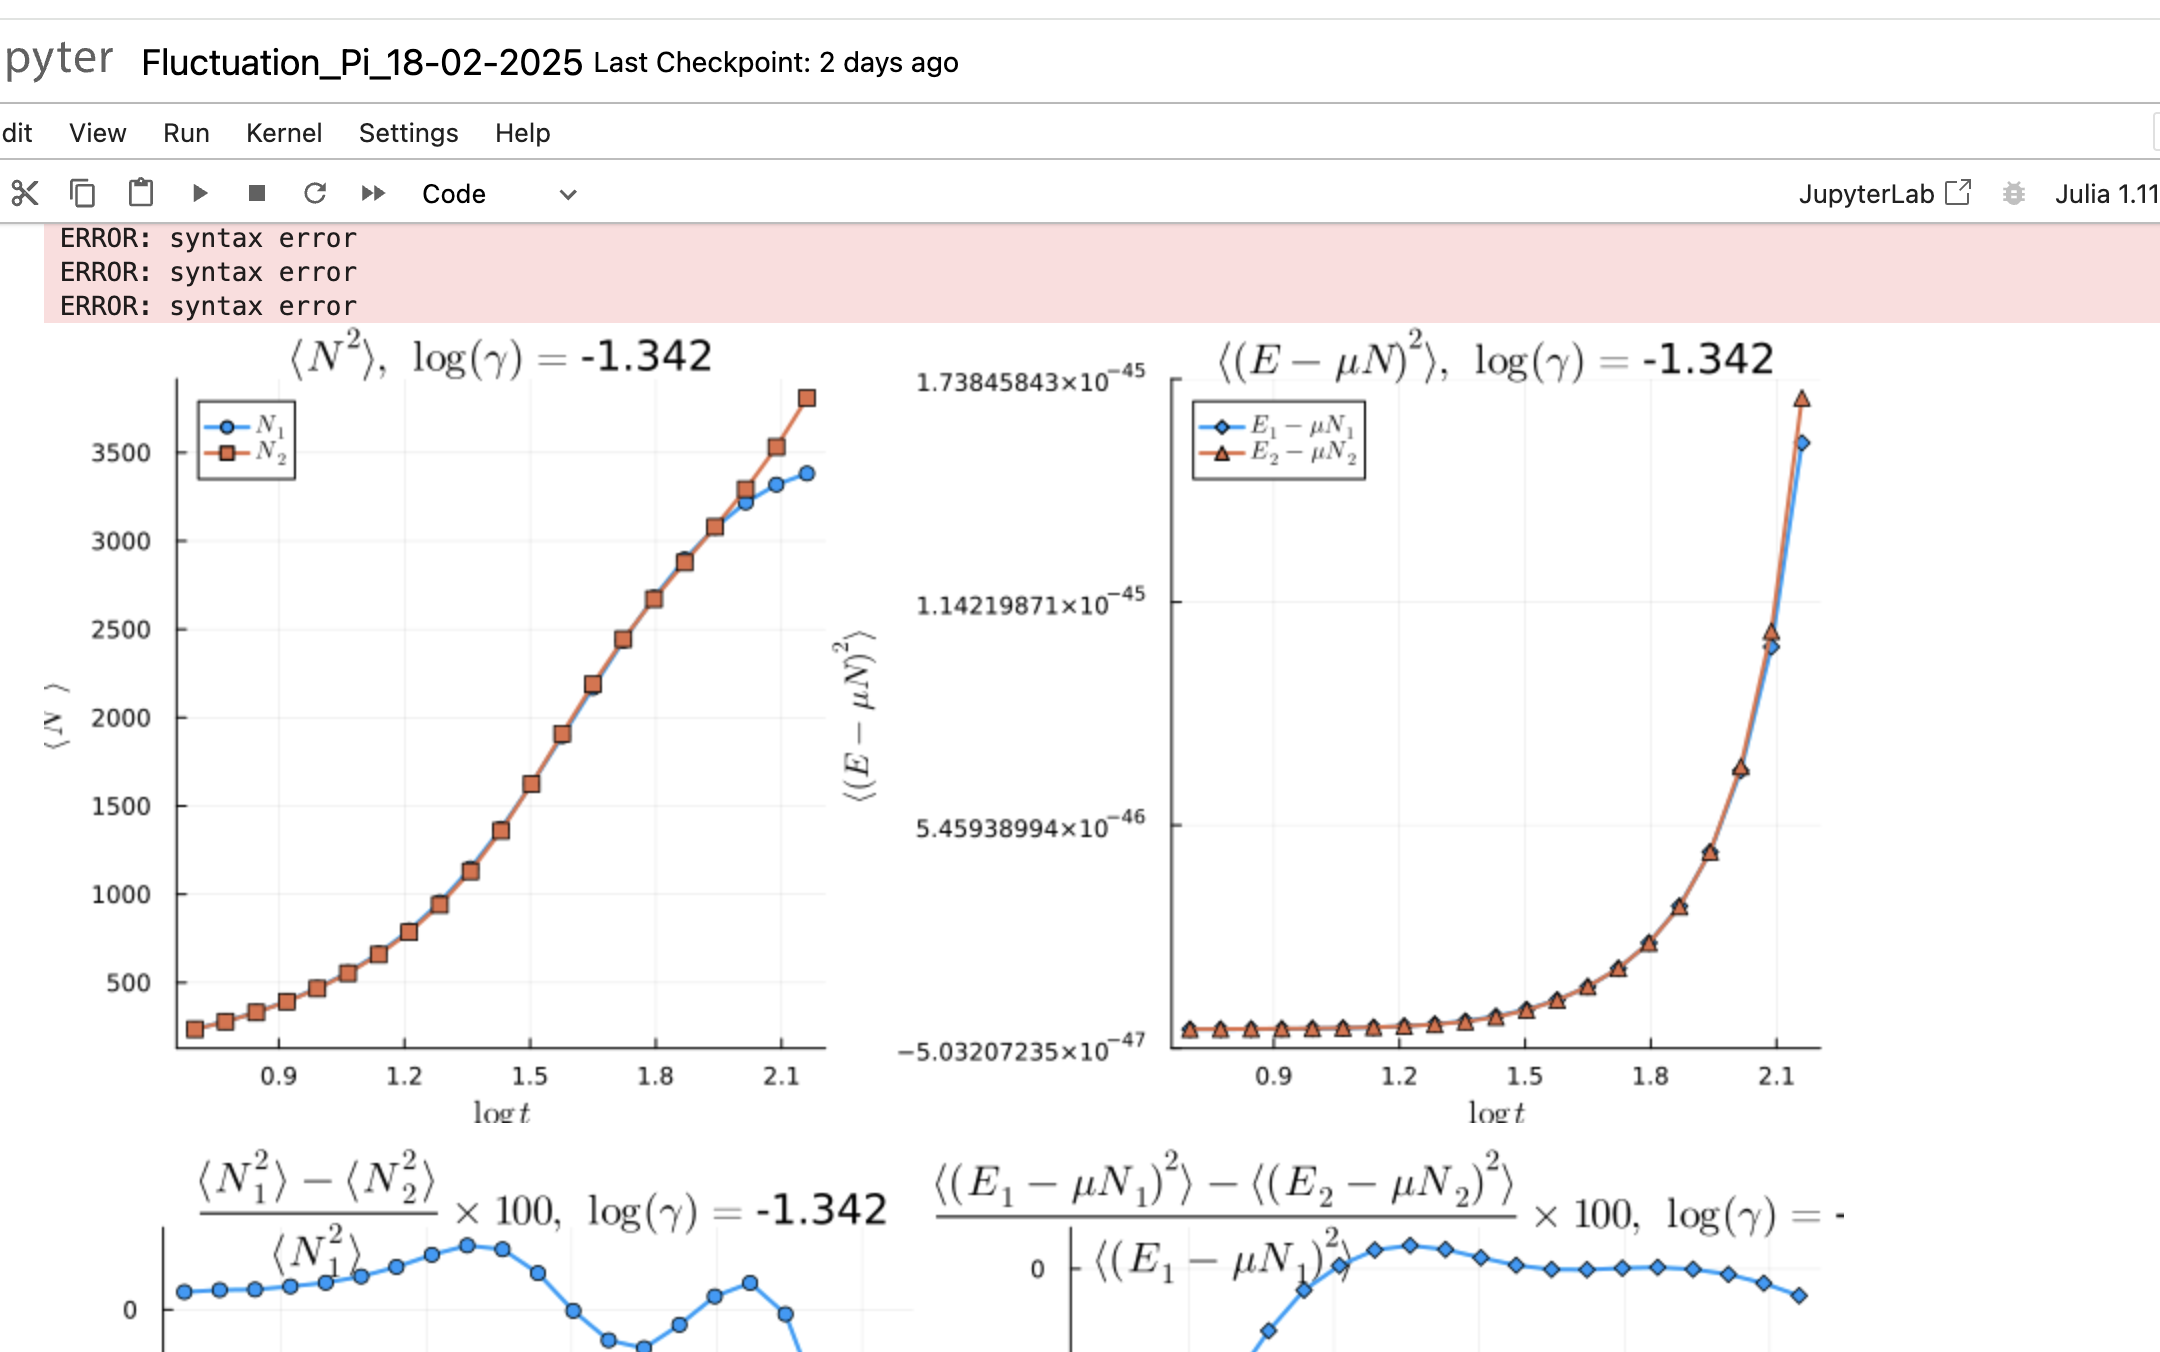
\includegraphics[width=1\textwidth]{Figures/test}

%\begin{aff}
%Donc une a l'ordre un en $\delta \theta (\operator{A}^{(0)})^{-1} %\operator{V}$ 

%\begin{eqnarray*}
%	\langle \delta \Pi ( \theta) \delta \Pi ( \theta') \rangle & = &  ( (\Pi^c_s - \Pi^c)\Pi^c/\Pi^c_s ) ( \theta ) \delta_{\theta, \theta'}/\delta \theta + \mathscr{F}(\theta , \theta' ) ,	
%\end{eqnarray*}

%avec 

%\begin{eqnarray*}
%	\mathscr{F}(\theta , \theta' ) & = & \left [ (\Pi^c_s - \Pi^c )( \theta)  +  (\Pi^c_s - \Pi^c ) ( \theta' )\right ] \frac{\Pi^c}{\Pi^c_s}(\theta)\frac{\Pi^c}{\Pi^c_s}(\theta') \frac{ \Delta( \theta'- \theta )}{ 2 \pi }\\
%	&&  - \left [ (\Pi^c_s - \Pi^c )( \theta)   (\Pi^c_s - \Pi^c ) ( \theta' )\right ] \frac{\Pi^c}{\Pi^c_s}(\theta)\frac{\Pi^c}{\Pi^c_s}(\theta')\int d\theta'' \left (   \frac{ \Pi^c/\Pi^c_s}{\Pi^c_s - \Pi^c} \right )(\theta'') \frac{\Delta(\theta''- \theta)}{2 \pi}\frac{\Delta(\theta''- \theta')}{2 \pi}  	
%\end{eqnarray*}
%\end{aff}



 









\chapter{Aaction de $\operator{H}$ sur l’état $\vert \psi_N\rangle$}
%Dans ce chapitre, nous nous intéressons aux fluctuations de la distribution de rapidité \( \delta \rho \) autour d'une distribution de référence \( \rho^c \), qui maximise la contribution à la fonction de partition des états, exprimée comme une fonctionnelle de la distribution \( \rho \) : 

La fonction de partition des états, s'exprime comme une fonctionnelle de la distribution \( \rho \) : 

\begin{eqnarray*}
	\Xi & = & \sum_\rho \exp \left( -\mathcal{A}(\rho) \right).
\end{eqnarray*}  

Dans la section {\em \bf Entropie de Yang-Yang} (\ref{??}), l'action \( \mathcal{A}(\rho) \) s'écrit sous la forme :  

\begin{eqnarray*}
	\mathcal{A}(\rho) & \doteq & - L\mathcal{S}_{YY}(\rho) + L\int f(\theta) \rho (\theta) \, d\theta,		
\end{eqnarray*}  

où \( \mathcal{S}_{YY} \) est la fonctionnelle d'entropie de Yang-Yang, définie dans (\ref{??}), et \( f \) est la fonction paramétrant les charges, introduite dans (\ref{??}).  

Dans cette même section {\em \bf Entropie de Yang-Yang} (\ref{??}), nous avons établi un lien entre \( f \) et distribution de référence \( \rho^c \), qui maximise la contribution à la fonction de partition des états .\\

On veux tester si nos experience est décrit pas un GGE. Pour cela nous nous intéressons aux fluctuations de la distribution de rapidité \( \delta \rho \) autour \( \rho^c \).

%Nous poursuivons à présent avec cette définition de l'action de classe $\mathcal{C}^2$ et admetant une distribution critique $\rho^c$ tel que sa différentielle en ce point critique soit nulle $d\mathcal{A}_{\rho^c} = 0 $ (\ref{??}) de sorte que d'aprés la formule de Taylor-Youg %afin de déterminer les fluctuations autour de \( \Pi^c \). Pour cela, nous réécrivons l'action sous la forme :  

Nous poursuivons à présent avec cette définition de l'action de classe $\mathcal{C}^2$ et admetant une distribution critique $\rho^c$ tel que sa différentielle en ce point critique soit nulle $d\mathcal{A}_{\rho^c} = 0 $ (\ref{??}) de sorte que d'aprés la formule de Taylor-Youg %afin de déterminer les fluctuations autour de \( \Pi^c \). Pour cela, nous réécrivons l'action sous la forme :  

\begin{eqnarray*}  
	\mathcal{A}(\rho^c + \delta \rho) & \underset{ \delta \rho \to 0 }{=} & \mathcal{A}(\rho^c)  + \frac{1}{2} \left. \frac{\delta^2 \mathcal{A}}{\delta \rho^2} \right|_{\rho^c} (\delta \rho) + \mathcal{O}((\delta \rho)^3),  
\end{eqnarray*}  

une expression quadratique pour l'action à l'ordre dominant en \( \delta \Pi \) avec $\left. \frac{\delta^2 \mathcal{A}}{\delta \rho^2} \right|_{\rho^c}$ la forme quadratique définie positive (Fig (\ref{fig.fluctu.A})).

\begin{figure}[H]
	\centering 
	\begin{tikzpicture}
		\begin{scope}[shift={(0,0)}]
			\begin{scope}[transform canvas={scale=0.6}]
				% Définition des couleurs avec les codes HTML
\definecolor{colorOne}{HTML}{443E46}
\definecolor{colorTwo}{HTML}{F6DEB8}
\definecolor{colorThree}{HTML}{908CA4}
\definecolor{colorFour}{HTML}{57659E}
\definecolor{colorFive}{HTML}{C57284}
\definecolor{colorSix}{HTML}{FF5B69}

% Raccourcis pour les couleurs
\def\colorOne{colorOne}
\def\colorTwo{colorTwo}
\def\colorThree{colorThree}
\def\colorFour{colorFour}
\def\colorFive{colorFive}
\def\colorSix{colorSix}

\def\colorslide{blue!50!black}



\begin{scope}
	% Tracer une courbe lisse entre des points
	\draw[shift={(0,0)} ,\colorOne]
		(-1 , 0 ) edge [thick,line width=0.8ex , ->,>=triangle 45  , \colorOne] node [pos = 1 , below ]{\huge$\rho$}( 5  , 0 )
	;
	\draw[shift={(0,0)}, color=\colorOne]
		(0, -1.0 ) edge [thick,line width=0.8ex , ->,>=triangle 45  ]node [pos=0.9,left=0.2cm ]{\huge$\mathcal{A}(\rho)$}( 0  , 5 )
	;
	\draw[]
		(2.5, 0.12 ) edge [thick,line width=0.8ex ,\colorThree ]node [pos=1,below  ]{\huge$\rho^c$} (2.5, -0.12 )	
	;
	
	\draw[]
		(2.5, -0.12 ) edge [thick,line width=0.4ex , dashed, \colorThree ] (2.5, 5.5 )
		(1.5, 1 ) edge [thick,line width=0.4ex , <->,>=triangle 45  , \colorThree ] (3.5, 1 )
		(-0.3,1) edge [thick,line width=0.4ex  , \colorThree ] node [pos=0,left ]{\huge$\mathcal{A}(\rho^c)$} (0.3, 1 )	
	;
    \draw[thick, line width=0.8ex , \colorFour] plot[smooth, tension=0.7] coordinates {
        (1, 5) (1.6 , 3 ) (2.5, 1) (3.5 , 3 )  (4, 5)
    };		
	
\end{scope}

	
			
			\end{scope}
			
			\draw[color = red , scale = 0.5 , draw = none  ] (-2 , -1) rectangle (5, 6) ; 	
		\end{scope}
		
		\begin{scope}[shift={(19,-1)}]
			\begin{scope}[transform canvas={scale=0.6}]
				% Définition des couleurs avec les codes HTML
\definecolor{colorOne}{HTML}{443E46}
\definecolor{colorTwo}{HTML}{F6DEB8}
\definecolor{colorThree}{HTML}{908CA4}
\definecolor{colorFour}{HTML}{57659E}
\definecolor{colorFive}{HTML}{C57284}
\definecolor{colorSix}{HTML}{FF5B69}

% Raccourcis pour les couleurs
\def\colorOne{colorOne}
\def\colorTwo{colorTwo}
\def\colorThree{colorThree}
\def\colorFour{colorFour}
\def\colorFive{colorFive}
\def\colorSix{colorSix}

\def\colorslide{blue!50!black}

\def\Occupation{
	\def\traitx{0.3}
	\def\traity{0.5}
	\draw[shift={(0,0)}]
		(-13.5 , 0 ) edge [thick,line width=0.8ex ]( -3.2  , 0 )
		( -3.2 - \traitx  , 0 - \traity ) edge [thick,line width=0.8ex ]( -3.2 + \traitx  , 0 + \traity  )
		( -2.8 - \traitx  , 0 - \traity ) edge [thick,line width=0.8ex ]( -2.8 + \traitx  , 0 + \traity  )
		(-2.8 , 0 ) edge [thick,line width=0.8ex ](2.8  , 0 )
		( 2.8 - \traitx  , 0 - \traity ) edge [thick,line width=0.8ex ]( 2.8 + \traitx  , 0 + \traity  )
		( 3.2 - \traitx  , 0 - \traity ) edge [thick,line width=0.8ex ]( 3.2 + \traitx  , 0 + \traity  )
		(3.2, 0 ) edge [thick,line width=0.8ex,->,>=triangle 45 , color = black ]node [pos=1.01,below  ]{\huge$\theta$}	( 13  , 0 )
	;
	\draw[shift={(0,0)}, color=\colorOne]
		(-10.5 , -1.5 ) edge [thick,line width=0.8ex , ->,>=triangle 45  ]( -10.5  , 4.5 )
	;
		
	\foreach \r in {1 , ... , 3 } {
%		\draw[
%		decoration={
%		markings,
%    	mark connection node=my node,
%    	mark=at position 0 with{\node [blue,transform shape] (my node) {\large \r};}},
%		color=gray, thick, 
%		line width=0.5ex] decorate { 
%            (-11.0, \r) -- (-10.1, \r )}
%        ;
        \draw[
			color=\colorOne,
			] 
            (-11.0, \r) edge[color=\colorThree , thick,line width=0.5ex] node [pos=-0.5 ]{\large\color{\colorFour} $\frac{\r}{\delta \theta}$ } (-10.3, \r )
        	;
	
	}
	

	
	% Graduation abcsisse 
	% Définitions des listes
% Definitions of the lists
\def\listetuple{-9/\theta_{1}, -8/\theta_{2} , -5/\theta_{3} , -2/\theta_{a-1} , 0/\theta_{a} , 1/\theta_{a+1} , 2/\theta_{a+2} ,  5/\theta_{N-4} , 7/\theta_{N-3},8/\theta_{N-1},9/\theta_{N} }
\def\listetrais{-12 , -11, -10, -9 , -8 , -7 ,  -6 , -5, -4.5,-4, -2 , -1, 0 , 0.5, 1, 2, 4 , 5 ,  6 , 7 , 8 ,8.5, 9 ,  10 , 11, 12 }

% Loop over listetrais
\foreach \r in \listetrais {
    % Initialize found variable to zero
    % Initialize found variable to zero
    %\pgfmathsetmacro\found{0}
    \global\def\found{0}
    \xdef\nomtheta{}
    
    % Check if \r is in listetuple
    \foreach \x/\y in \listetuple { 
        \ifdim \r pt=\x pt % If \r matches any \x in listetuple
            \global\def\found{1} ;
            \xdef\nomtheta{\y} % Set \nomtheta to the corresponding \y
            %\pgfmathsetmacro\found{1} % Set found to 1            
            %\global\pgfmathsetmacro\found{1}
        \fi
    }
    
    %\node [circle, draw, red] (A) at (\r, 2) {\found , $\nomtheta$};
    
    % Draw the line and display \nomtheta if found
    \ifnum\found=1
        \draw[color=\colorOne, thick, line width=0.5ex] 
            (\r, -0.3) -- (\r, 0.3) node[red , pos=-0.5] {\large $\nomtheta$};
         \filldraw[line width=0.5ex, color=\colorSix, outer color=\colorSix, inner color=\colorSix] 
            (\r, 0) circle (4pt);
    \else 
        % Draw without \nomtheta and add a blue circle if not found
        \draw[color=\colorOne, thick, line width=0.5ex] 
            (\r, -0.3) -- (\r, 0.3);
        \filldraw[line width=0.5ex, color=\colorSix, outer color=\colorTwo, inner color=\colorTwo] 
            (\r, 0) circle (4pt); 
    \fi
}

\def\listetrais{-9.5/\theta_{i-1}/2/3, -6.5/\theta_{i}/1/4  ,   -1.5/\theta_{j}/2/4 , 1.5/\theta_{j+1}/-1/3 , 3.5/\theta_{\ell-1}/1/3 , 6.5/\theta_{\ell}/3/4 , 9.5/\theta(\theta_{\ell+1})/-1/3 };



\foreach \r/\nomx/\y/\ys in \listetrais {
	\draw[
		decoration={
		markings,
    	mark connection node=my node,
    	mark=at position .5 with{\node [blue,transform shape] (my node) {\large \color{\colorFour} $\nomx$};}},
		color=\colorThree , thick, 
		line width=0.5ex] decorate { 
            (\r, 0.12) -- (\r, -1.2)}
        ;
     
     \ifdim \y pt > -1 pt 
     	\draw[
			decoration={
			markings,
    		mark connection node=my node,
    		mark=at position .5 with{\node [blue,transform shape] (my node) {\large \color{\colorFour} $\Pi(\nomx) $};}},
			color=\colorThree, thick, 
			line width=0.5ex] decorate { 
            (\r, \y) -- (\r +3, \y)}
        ;
        \draw[
			decoration={
			markings,
    		mark connection node=my node,
    		mark=at position .5 with{\node [blue,transform shape] (my node) {\large \color{\colorFive} $\Pi_s(\nomx) $};}},
			color=\colorFive, thick, 
			line width=0.5ex] decorate { 
            (\r, \ys) -- (\r +3, \ys)}
        ;
     \fi 
     \ifdim \r pt= -1.5 pt
     	\draw[
     		decoration={
			markings,
    		mark connection node=my node,
    		mark=at position .5 with{\node [blue,transform shape] (my node) {\large \color{\colorFour}  $\delta \theta $};},
    		%mark=at position 0.1  with {\arrow[blue, line width=0.5ex]{<}},
    		%mark=at position 1  with {\arrow[blue, line width=0.5ex]{>}}
    		},
        	color=\colorThree,
        	thick,
        	line width=0.5ex,
        	%arrows={Computer Modern Rightarrow[line cap=round]-Computer Modern Rightarrow[line cap=round]}
   			](\r, -1.2) edge[arrows={Computer Modern Rightarrow[line cap=round]-}] (\r + 0.4, -1.2)decorate {
    		(\r, -1.2) -- (\r + 3, -1.2)}(\r + 2, -1.2) edge[arrows={-Computer Modern Rightarrow[line cap=round]}] (\r + 3, -1.2)
    		;
    \fi
			
	
}


			
}


\begin{scope}
	%\draw[help lines , width=1.5ex] (-8,-3) grid (8,3);\draw[help lines ,width=0.5ex , opacity = 0.5] (-3,-3) grid[step=0.1] (3,3));
	
	%\draw[help lines] 
	%	(-3,-3) edge[width=1.5ex] grid (3,3)	
	%	(-3,-3) edge[width=0.5ex , opacity = 0.5] grid (3,3)	
	%;
	\begin{scope}[shift={(0,1)},rotate=0,opacity=1,color=black]
		\Occupation	
		
		%\node[anchor=east, font=\bfseries] at (-11, 0) {\color{red}\large (T = 0 )} ;	
	\end{scope}
	
	
	
	
	\begin{scope}[shift={(-10.5,7)},rotate=0,opacity=1,color=black]
	
	\begin{scope}[shift={(-0,0)},rotate=0,opacity=1,color=black]
	
		\draw[shift={(0,0)} ,line width=1ex,rounded corners = 1ex,color=\colorOne , opacity =1 ,fill=\colorOne!00 , pattern={north east lines} , pattern color=\colorOne!00 ]
			(0 , -1 ) rectangle (5,1)
		;
		

		\begin{scope}[shift={(0.5,0.5)}]
			\draw[color=\colorOne, thick, line width=0.5ex] 
            (0, -0.3) -- (0, 0.3) ;
            \filldraw[line width=0.5ex, color=\colorSix, outer color=\colorSix, inner color=\colorSix] 
            (0, 0) circle (4pt);
            
            \node[anchor=west, font=\bfseries] at (0.2, 0) {\color{\colorSix}\large : quasi-particule};
		\end{scope}
		
		\begin{scope}[shift={(0.5,-0.5)}]
			\draw[color=\colorOne, thick, line width=0.5ex] 
            (0, -0.3) -- (0, 0.3) ;
            \filldraw[line width=0.5ex, color=\colorSix, outer color=\colorTwo, inner color=\colorTwo] 
            (0, 0) circle (4pt);
            
            \node[anchor=west, font=\bfseries] at (0.2, 0) {\color{\colorSix}\large : hole};
		\end{scope}

	\end{scope}
	
	\begin{scope}[shift={(6,0)},rotate=0,opacity=1,color=black]	
		
		\draw[shift={(0,0)} ,line width=1ex,rounded corners = 1ex,color=\colorOne , opacity =1 ,fill=\colorOne!00 , pattern={north east lines} , pattern color=\colorOne!00 ]
			(0 , -1 ) rectangle (7.5,1)
		;
		
		\node[anchor=west] at (0.5, 0.5) {\color{\colorFour}\large $\Pi$ };\node[anchor=west, font=\bfseries] at (1, 0.5) {\color{\colorFour}\large : quasi-particule distribution};
		
		\node[anchor=west] at (0.5, -0.5) {\color{\colorFour}\large $\Pi_h$ };\node[anchor=west, font=\bfseries] at (1, -0.5) {\color{\colorFour}\large  : hole distribution};
		
	\end{scope}
	
	\begin{scope}[shift={(14.5,0)},rotate=0,opacity=1,color=black]	
		
		\draw[shift={(0,0)} ,line width=1ex,rounded corners = 1ex,color=\colorOne , opacity =1 ,fill=\colorOne!00 , pattern={north east lines} , pattern color=\colorOne!00 ]
			(0 , -0.5 ) rectangle (7.0,0.5)
		;
		
		\node[anchor=west] at (0.2, 0) {\color{\colorFour}\large ${\color{\colorFive}\Pi_s} = \Pi + \Pi_h $ } node[anchor=west , font=\bfseries] at (3.1 , 0 )  {\color{\colorFour}\large {\color{\colorFive} : density of states}};
		
	\end{scope}
	
	
	\end{scope}


		
	
\end{scope}

	
			
			\end{scope}
			\begin{scope}[scale=1]
				\draw[color = red , scale = 1 , draw = none  ] (-1 , -1) rectangle (5, 5) ; 
			\end{scope}	
		\end{scope}

		
				
			
	\end{tikzpicture}	
	\captionsetup{skip=10pt} % Ajoute de l’espace après la légende
	\label{fig.fluctu.A}
\end{figure}


On discrétise l'axe des rapidités en  petite cellule de rapidité $[\theta, \theta+\delta\theta]$, qui contient $L\rho(\theta) \delta \theta$ rapidités. 
	



Avec ces petites tranches, la forme quadratique s’écrit :

\begin{eqnarray*}
    \left. \frac{\delta^2 \mathcal{A}}{{\delta \rho}^2} \right|_{\rho^c}(\delta \rho ) &=&  \sum_{a,b \mid \text{tranche}}  
    \delta \rho(\theta_a)  \frac{\partial^2 \mathcal{A}}{\partial \delta \rho(\theta_a) \partial \delta \rho(\theta_b) } (\rho^c)  \delta \rho(\theta_b).
\end{eqnarray*}
Les fluctuations s’écrivent donc :

\begin{eqnarray*}
    \langle \delta \rho ( \theta) \delta \rho ( \theta') \rangle &=&  
    \frac{ \int d\delta \rho \, \delta \rho(\theta) \delta \rho ( \theta') 
    \exp \left( - \frac{1}{2} \sum_{a,b \mid \text{tranche}}  
    \delta \rho(\theta_a) \frac{\partial^2 \mathcal{A}}{\partial \delta \rho(\theta_a) \partial \delta \rho(\theta_b) } (\rho^c)  \delta \rho(\theta_b) \right) }
    { \int d\delta \Pi  
    \exp \left( - \frac{1}{2} \sum_{a,b \mid \text{tranche}}  
    \delta \rho(\theta_a) \frac{\partial^2 \mathcal{A}}{\partial \delta \rho(\theta_a) \partial \delta \rho(\theta_b) } (\rho^c)  \delta \rho(\theta_b) \right) } \\
    &=& \left( \mathbf{A}^{-1} \right)_{\theta , \theta'}
\end{eqnarray*}


\begin{aff}

\begin{eqnarray*}
	\langle \delta \rho ( \theta) \delta \rho ( \theta') \rangle &=& 	\left( \mathbf{A}^{-1} \right)_{\theta , \theta'}
\end{eqnarray*}

	
avec la  {\em matrice hessienne} $\mathbf{A}_{\theta , \theta'} \equiv \frac{\partial^2 \mathcal{A}}{\partial \delta \rho(\theta) \partial \delta \rho(\theta') }(\rho^c)$, au point critique/ qui maximise la probabilité  $\rho^c=\rho^c_s \nu^c $, s'écrit

\begin{eqnarray*}
	\operator{A} & = & \operator{A}^{(0)} + \delta \theta \operator{V}
\end{eqnarray*}

avec 

\begin{eqnarray*}
	A^{(0)}_{\theta , \theta'}  & = &  L\delta \theta \left ( \frac{ 1}{\rho^c_s ( 1  - \nu^c ) \nu^c } \right )(\theta)    \delta({\theta - \theta '})	,\\
	V_{\theta , \theta'}  &= & L \delta \theta \left \{ - \left [ \left ( \frac{1}{\rho^c_s( 1 - \nu^c) } \right ) ( \theta)  +  \left ( \frac{1}{\rho^c_s( 1 - \nu^c) } \right ) ( \theta' )\right ] \frac{ \Delta( \theta'- \theta )}{ 2 \pi } + \int d\theta''  \left ( \frac{\nu^c}{\rho^c_s( 1 - \nu^c) } \right )(\theta'') \frac{\Delta(\theta''- \theta)}{2 \pi}\frac{\Delta(\theta''- \theta')}{2 \pi}   \right \} 	
\end{eqnarray*}

\end{aff}

\subsection{Testes}

\begin{eqnarray*}
	\Delta_{\operator{\mathcal{N}}}^2  & = &  \frac{1}{\beta} \left . \frac{\partial \langle \operator{\mathcal{N}} \rangle}{\partial \mu} \right )_T \\
	\Delta_{\operator{\mathcal{E}}-\mu \operator{\mathcal{N}}}^2  & = &  - \left . \frac{\partial \langle \operator{\mathcal{E}}-\mu \operator{\mathcal{N}} \rangle}{\partial \beta} \right )_\mu 
\end{eqnarray*}

et 

\begin{eqnarray*}
	\Delta_{\operator{\mathcal{N}}}^2  &= & L^2 \int d\theta_a \int d \theta_b \, \langle \delta \rho(\theta_a) \delta \rho(\theta_b) \rangle \\
	\Delta_{\operator{\mathcal{E}}-\mu \operator{\mathcal{N}}}^2  & = & L^2 \int d\theta_a \int d \theta_b \, \left ( - \mu + \frac{1}2 m \theta_a^2  \right  )\left ( - \mu + \frac{1}2 m \theta_b^2  \right  )  \langle \delta \rho(\theta_a) \delta \rho(\theta_b) \rangle
\end{eqnarray*}

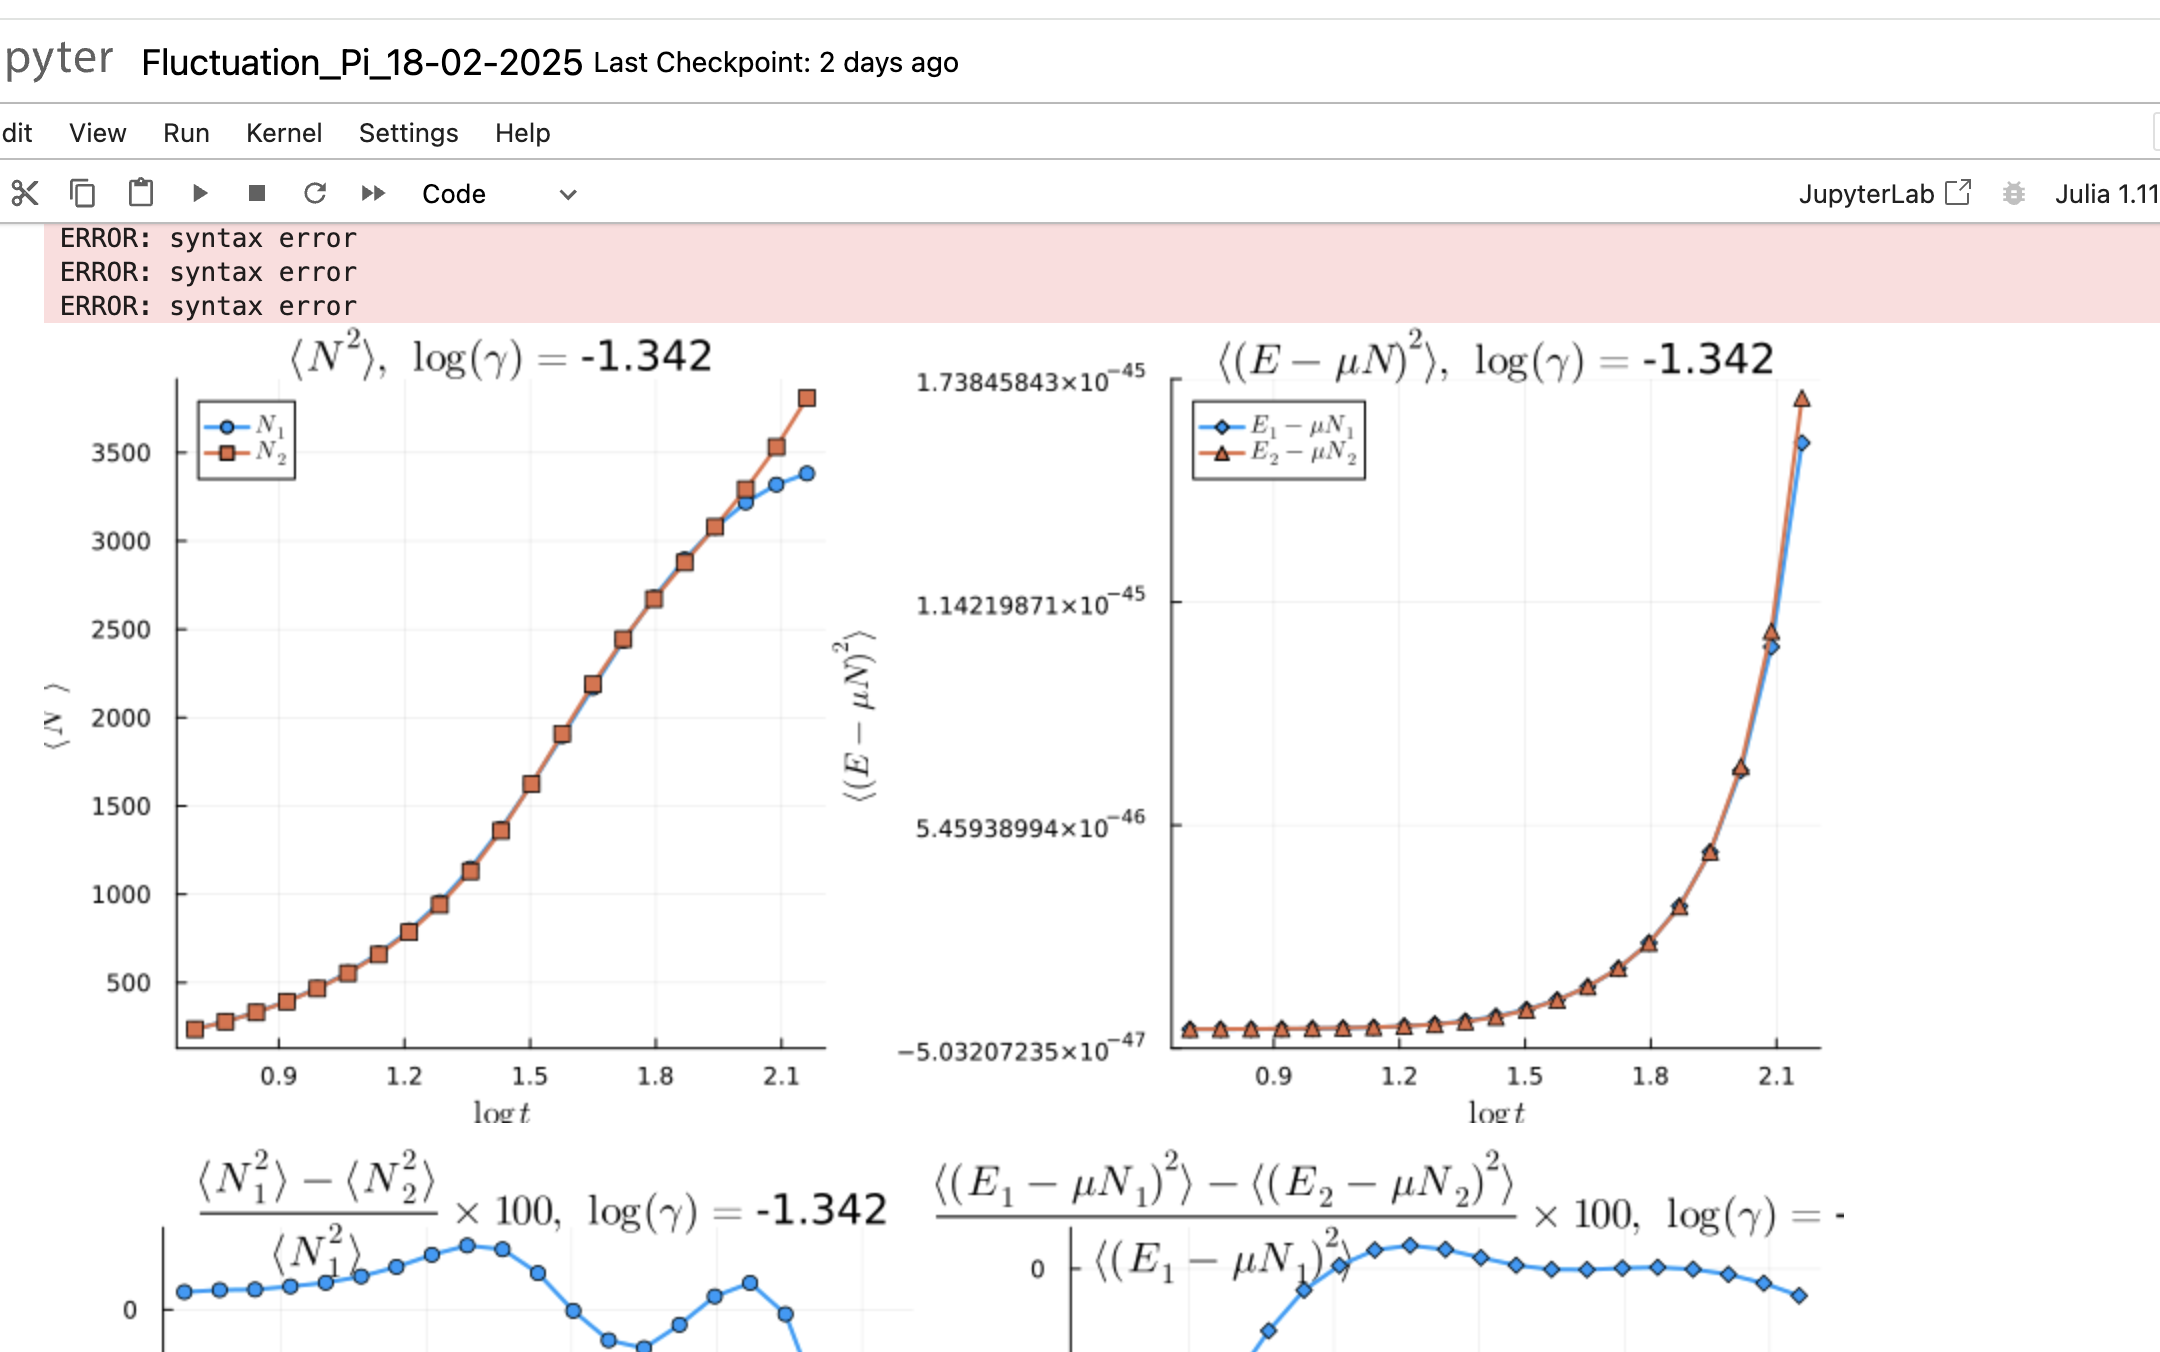
\includegraphics[width=1\textwidth]{Figures/test}

%\begin{aff}
%Donc une a l'ordre un en $\delta \theta (\operator{A}^{(0)})^{-1} %\operator{V}$ 

%\begin{eqnarray*}
%	\langle \delta \Pi ( \theta) \delta \Pi ( \theta') \rangle & = &  ( (\Pi^c_s - \Pi^c)\Pi^c/\Pi^c_s ) ( \theta ) \delta_{\theta, \theta'}/\delta \theta + \mathscr{F}(\theta , \theta' ) ,	
%\end{eqnarray*}

%avec 

%\begin{eqnarray*}
%	\mathscr{F}(\theta , \theta' ) & = & \left [ (\Pi^c_s - \Pi^c )( \theta)  +  (\Pi^c_s - \Pi^c ) ( \theta' )\right ] \frac{\Pi^c}{\Pi^c_s}(\theta)\frac{\Pi^c}{\Pi^c_s}(\theta') \frac{ \Delta( \theta'- \theta )}{ 2 \pi }\\
%	&&  - \left [ (\Pi^c_s - \Pi^c )( \theta)   (\Pi^c_s - \Pi^c ) ( \theta' )\right ] \frac{\Pi^c}{\Pi^c_s}(\theta)\frac{\Pi^c}{\Pi^c_s}(\theta')\int d\theta'' \left (   \frac{ \Pi^c/\Pi^c_s}{\Pi^c_s - \Pi^c} \right )(\theta'') \frac{\Delta(\theta''- \theta)}{2 \pi}\frac{\Delta(\theta''- \theta')}{2 \pi}  	
%\end{eqnarray*}
%\end{aff}



 









\chapter{Vérification explicite de la condition aux limites}
%Dans ce chapitre, nous nous intéressons aux fluctuations de la distribution de rapidité \( \delta \rho \) autour d'une distribution de référence \( \rho^c \), qui maximise la contribution à la fonction de partition des états, exprimée comme une fonctionnelle de la distribution \( \rho \) : 

La fonction de partition des états, s'exprime comme une fonctionnelle de la distribution \( \rho \) : 

\begin{eqnarray*}
	\Xi & = & \sum_\rho \exp \left( -\mathcal{A}(\rho) \right).
\end{eqnarray*}  

Dans la section {\em \bf Entropie de Yang-Yang} (\ref{??}), l'action \( \mathcal{A}(\rho) \) s'écrit sous la forme :  

\begin{eqnarray*}
	\mathcal{A}(\rho) & \doteq & - L\mathcal{S}_{YY}(\rho) + L\int f(\theta) \rho (\theta) \, d\theta,		
\end{eqnarray*}  

où \( \mathcal{S}_{YY} \) est la fonctionnelle d'entropie de Yang-Yang, définie dans (\ref{??}), et \( f \) est la fonction paramétrant les charges, introduite dans (\ref{??}).  

Dans cette même section {\em \bf Entropie de Yang-Yang} (\ref{??}), nous avons établi un lien entre \( f \) et distribution de référence \( \rho^c \), qui maximise la contribution à la fonction de partition des états .\\

On veux tester si nos experience est décrit pas un GGE. Pour cela nous nous intéressons aux fluctuations de la distribution de rapidité \( \delta \rho \) autour \( \rho^c \).

%Nous poursuivons à présent avec cette définition de l'action de classe $\mathcal{C}^2$ et admetant une distribution critique $\rho^c$ tel que sa différentielle en ce point critique soit nulle $d\mathcal{A}_{\rho^c} = 0 $ (\ref{??}) de sorte que d'aprés la formule de Taylor-Youg %afin de déterminer les fluctuations autour de \( \Pi^c \). Pour cela, nous réécrivons l'action sous la forme :  

Nous poursuivons à présent avec cette définition de l'action de classe $\mathcal{C}^2$ et admetant une distribution critique $\rho^c$ tel que sa différentielle en ce point critique soit nulle $d\mathcal{A}_{\rho^c} = 0 $ (\ref{??}) de sorte que d'aprés la formule de Taylor-Youg %afin de déterminer les fluctuations autour de \( \Pi^c \). Pour cela, nous réécrivons l'action sous la forme :  

\begin{eqnarray*}  
	\mathcal{A}(\rho^c + \delta \rho) & \underset{ \delta \rho \to 0 }{=} & \mathcal{A}(\rho^c)  + \frac{1}{2} \left. \frac{\delta^2 \mathcal{A}}{\delta \rho^2} \right|_{\rho^c} (\delta \rho) + \mathcal{O}((\delta \rho)^3),  
\end{eqnarray*}  

une expression quadratique pour l'action à l'ordre dominant en \( \delta \Pi \) avec $\left. \frac{\delta^2 \mathcal{A}}{\delta \rho^2} \right|_{\rho^c}$ la forme quadratique définie positive (Fig (\ref{fig.fluctu.A})).

\begin{figure}[H]
	\centering 
	\begin{tikzpicture}
		\begin{scope}[shift={(0,0)}]
			\begin{scope}[transform canvas={scale=0.6}]
				% Définition des couleurs avec les codes HTML
\definecolor{colorOne}{HTML}{443E46}
\definecolor{colorTwo}{HTML}{F6DEB8}
\definecolor{colorThree}{HTML}{908CA4}
\definecolor{colorFour}{HTML}{57659E}
\definecolor{colorFive}{HTML}{C57284}
\definecolor{colorSix}{HTML}{FF5B69}

% Raccourcis pour les couleurs
\def\colorOne{colorOne}
\def\colorTwo{colorTwo}
\def\colorThree{colorThree}
\def\colorFour{colorFour}
\def\colorFive{colorFive}
\def\colorSix{colorSix}

\def\colorslide{blue!50!black}



\begin{scope}
	% Tracer une courbe lisse entre des points
	\draw[shift={(0,0)} ,\colorOne]
		(-1 , 0 ) edge [thick,line width=0.8ex , ->,>=triangle 45  , \colorOne] node [pos = 1 , below ]{\huge$\rho$}( 5  , 0 )
	;
	\draw[shift={(0,0)}, color=\colorOne]
		(0, -1.0 ) edge [thick,line width=0.8ex , ->,>=triangle 45  ]node [pos=0.9,left=0.2cm ]{\huge$\mathcal{A}(\rho)$}( 0  , 5 )
	;
	\draw[]
		(2.5, 0.12 ) edge [thick,line width=0.8ex ,\colorThree ]node [pos=1,below  ]{\huge$\rho^c$} (2.5, -0.12 )	
	;
	
	\draw[]
		(2.5, -0.12 ) edge [thick,line width=0.4ex , dashed, \colorThree ] (2.5, 5.5 )
		(1.5, 1 ) edge [thick,line width=0.4ex , <->,>=triangle 45  , \colorThree ] (3.5, 1 )
		(-0.3,1) edge [thick,line width=0.4ex  , \colorThree ] node [pos=0,left ]{\huge$\mathcal{A}(\rho^c)$} (0.3, 1 )	
	;
    \draw[thick, line width=0.8ex , \colorFour] plot[smooth, tension=0.7] coordinates {
        (1, 5) (1.6 , 3 ) (2.5, 1) (3.5 , 3 )  (4, 5)
    };		
	
\end{scope}

	
			
			\end{scope}
			
			\draw[color = red , scale = 0.5 , draw = none  ] (-2 , -1) rectangle (5, 6) ; 	
		\end{scope}
		
		\begin{scope}[shift={(19,-1)}]
			\begin{scope}[transform canvas={scale=0.6}]
				% Définition des couleurs avec les codes HTML
\definecolor{colorOne}{HTML}{443E46}
\definecolor{colorTwo}{HTML}{F6DEB8}
\definecolor{colorThree}{HTML}{908CA4}
\definecolor{colorFour}{HTML}{57659E}
\definecolor{colorFive}{HTML}{C57284}
\definecolor{colorSix}{HTML}{FF5B69}

% Raccourcis pour les couleurs
\def\colorOne{colorOne}
\def\colorTwo{colorTwo}
\def\colorThree{colorThree}
\def\colorFour{colorFour}
\def\colorFive{colorFive}
\def\colorSix{colorSix}

\def\colorslide{blue!50!black}

\def\Occupation{
	\def\traitx{0.3}
	\def\traity{0.5}
	\draw[shift={(0,0)}]
		(-13.5 , 0 ) edge [thick,line width=0.8ex ]( -3.2  , 0 )
		( -3.2 - \traitx  , 0 - \traity ) edge [thick,line width=0.8ex ]( -3.2 + \traitx  , 0 + \traity  )
		( -2.8 - \traitx  , 0 - \traity ) edge [thick,line width=0.8ex ]( -2.8 + \traitx  , 0 + \traity  )
		(-2.8 , 0 ) edge [thick,line width=0.8ex ](2.8  , 0 )
		( 2.8 - \traitx  , 0 - \traity ) edge [thick,line width=0.8ex ]( 2.8 + \traitx  , 0 + \traity  )
		( 3.2 - \traitx  , 0 - \traity ) edge [thick,line width=0.8ex ]( 3.2 + \traitx  , 0 + \traity  )
		(3.2, 0 ) edge [thick,line width=0.8ex,->,>=triangle 45 , color = black ]node [pos=1.01,below  ]{\huge$\theta$}	( 13  , 0 )
	;
	\draw[shift={(0,0)}, color=\colorOne]
		(-10.5 , -1.5 ) edge [thick,line width=0.8ex , ->,>=triangle 45  ]( -10.5  , 4.5 )
	;
		
	\foreach \r in {1 , ... , 3 } {
%		\draw[
%		decoration={
%		markings,
%    	mark connection node=my node,
%    	mark=at position 0 with{\node [blue,transform shape] (my node) {\large \r};}},
%		color=gray, thick, 
%		line width=0.5ex] decorate { 
%            (-11.0, \r) -- (-10.1, \r )}
%        ;
        \draw[
			color=\colorOne,
			] 
            (-11.0, \r) edge[color=\colorThree , thick,line width=0.5ex] node [pos=-0.5 ]{\large\color{\colorFour} $\frac{\r}{\delta \theta}$ } (-10.3, \r )
        	;
	
	}
	

	
	% Graduation abcsisse 
	% Définitions des listes
% Definitions of the lists
\def\listetuple{-9/\theta_{1}, -8/\theta_{2} , -5/\theta_{3} , -2/\theta_{a-1} , 0/\theta_{a} , 1/\theta_{a+1} , 2/\theta_{a+2} ,  5/\theta_{N-4} , 7/\theta_{N-3},8/\theta_{N-1},9/\theta_{N} }
\def\listetrais{-12 , -11, -10, -9 , -8 , -7 ,  -6 , -5, -4.5,-4, -2 , -1, 0 , 0.5, 1, 2, 4 , 5 ,  6 , 7 , 8 ,8.5, 9 ,  10 , 11, 12 }

% Loop over listetrais
\foreach \r in \listetrais {
    % Initialize found variable to zero
    % Initialize found variable to zero
    %\pgfmathsetmacro\found{0}
    \global\def\found{0}
    \xdef\nomtheta{}
    
    % Check if \r is in listetuple
    \foreach \x/\y in \listetuple { 
        \ifdim \r pt=\x pt % If \r matches any \x in listetuple
            \global\def\found{1} ;
            \xdef\nomtheta{\y} % Set \nomtheta to the corresponding \y
            %\pgfmathsetmacro\found{1} % Set found to 1            
            %\global\pgfmathsetmacro\found{1}
        \fi
    }
    
    %\node [circle, draw, red] (A) at (\r, 2) {\found , $\nomtheta$};
    
    % Draw the line and display \nomtheta if found
    \ifnum\found=1
        \draw[color=\colorOne, thick, line width=0.5ex] 
            (\r, -0.3) -- (\r, 0.3) node[red , pos=-0.5] {\large $\nomtheta$};
         \filldraw[line width=0.5ex, color=\colorSix, outer color=\colorSix, inner color=\colorSix] 
            (\r, 0) circle (4pt);
    \else 
        % Draw without \nomtheta and add a blue circle if not found
        \draw[color=\colorOne, thick, line width=0.5ex] 
            (\r, -0.3) -- (\r, 0.3);
        \filldraw[line width=0.5ex, color=\colorSix, outer color=\colorTwo, inner color=\colorTwo] 
            (\r, 0) circle (4pt); 
    \fi
}

\def\listetrais{-9.5/\theta_{i-1}/2/3, -6.5/\theta_{i}/1/4  ,   -1.5/\theta_{j}/2/4 , 1.5/\theta_{j+1}/-1/3 , 3.5/\theta_{\ell-1}/1/3 , 6.5/\theta_{\ell}/3/4 , 9.5/\theta(\theta_{\ell+1})/-1/3 };



\foreach \r/\nomx/\y/\ys in \listetrais {
	\draw[
		decoration={
		markings,
    	mark connection node=my node,
    	mark=at position .5 with{\node [blue,transform shape] (my node) {\large \color{\colorFour} $\nomx$};}},
		color=\colorThree , thick, 
		line width=0.5ex] decorate { 
            (\r, 0.12) -- (\r, -1.2)}
        ;
     
     \ifdim \y pt > -1 pt 
     	\draw[
			decoration={
			markings,
    		mark connection node=my node,
    		mark=at position .5 with{\node [blue,transform shape] (my node) {\large \color{\colorFour} $\Pi(\nomx) $};}},
			color=\colorThree, thick, 
			line width=0.5ex] decorate { 
            (\r, \y) -- (\r +3, \y)}
        ;
        \draw[
			decoration={
			markings,
    		mark connection node=my node,
    		mark=at position .5 with{\node [blue,transform shape] (my node) {\large \color{\colorFive} $\Pi_s(\nomx) $};}},
			color=\colorFive, thick, 
			line width=0.5ex] decorate { 
            (\r, \ys) -- (\r +3, \ys)}
        ;
     \fi 
     \ifdim \r pt= -1.5 pt
     	\draw[
     		decoration={
			markings,
    		mark connection node=my node,
    		mark=at position .5 with{\node [blue,transform shape] (my node) {\large \color{\colorFour}  $\delta \theta $};},
    		%mark=at position 0.1  with {\arrow[blue, line width=0.5ex]{<}},
    		%mark=at position 1  with {\arrow[blue, line width=0.5ex]{>}}
    		},
        	color=\colorThree,
        	thick,
        	line width=0.5ex,
        	%arrows={Computer Modern Rightarrow[line cap=round]-Computer Modern Rightarrow[line cap=round]}
   			](\r, -1.2) edge[arrows={Computer Modern Rightarrow[line cap=round]-}] (\r + 0.4, -1.2)decorate {
    		(\r, -1.2) -- (\r + 3, -1.2)}(\r + 2, -1.2) edge[arrows={-Computer Modern Rightarrow[line cap=round]}] (\r + 3, -1.2)
    		;
    \fi
			
	
}


			
}


\begin{scope}
	%\draw[help lines , width=1.5ex] (-8,-3) grid (8,3);\draw[help lines ,width=0.5ex , opacity = 0.5] (-3,-3) grid[step=0.1] (3,3));
	
	%\draw[help lines] 
	%	(-3,-3) edge[width=1.5ex] grid (3,3)	
	%	(-3,-3) edge[width=0.5ex , opacity = 0.5] grid (3,3)	
	%;
	\begin{scope}[shift={(0,1)},rotate=0,opacity=1,color=black]
		\Occupation	
		
		%\node[anchor=east, font=\bfseries] at (-11, 0) {\color{red}\large (T = 0 )} ;	
	\end{scope}
	
	
	
	
	\begin{scope}[shift={(-10.5,7)},rotate=0,opacity=1,color=black]
	
	\begin{scope}[shift={(-0,0)},rotate=0,opacity=1,color=black]
	
		\draw[shift={(0,0)} ,line width=1ex,rounded corners = 1ex,color=\colorOne , opacity =1 ,fill=\colorOne!00 , pattern={north east lines} , pattern color=\colorOne!00 ]
			(0 , -1 ) rectangle (5,1)
		;
		

		\begin{scope}[shift={(0.5,0.5)}]
			\draw[color=\colorOne, thick, line width=0.5ex] 
            (0, -0.3) -- (0, 0.3) ;
            \filldraw[line width=0.5ex, color=\colorSix, outer color=\colorSix, inner color=\colorSix] 
            (0, 0) circle (4pt);
            
            \node[anchor=west, font=\bfseries] at (0.2, 0) {\color{\colorSix}\large : quasi-particule};
		\end{scope}
		
		\begin{scope}[shift={(0.5,-0.5)}]
			\draw[color=\colorOne, thick, line width=0.5ex] 
            (0, -0.3) -- (0, 0.3) ;
            \filldraw[line width=0.5ex, color=\colorSix, outer color=\colorTwo, inner color=\colorTwo] 
            (0, 0) circle (4pt);
            
            \node[anchor=west, font=\bfseries] at (0.2, 0) {\color{\colorSix}\large : hole};
		\end{scope}

	\end{scope}
	
	\begin{scope}[shift={(6,0)},rotate=0,opacity=1,color=black]	
		
		\draw[shift={(0,0)} ,line width=1ex,rounded corners = 1ex,color=\colorOne , opacity =1 ,fill=\colorOne!00 , pattern={north east lines} , pattern color=\colorOne!00 ]
			(0 , -1 ) rectangle (7.5,1)
		;
		
		\node[anchor=west] at (0.5, 0.5) {\color{\colorFour}\large $\Pi$ };\node[anchor=west, font=\bfseries] at (1, 0.5) {\color{\colorFour}\large : quasi-particule distribution};
		
		\node[anchor=west] at (0.5, -0.5) {\color{\colorFour}\large $\Pi_h$ };\node[anchor=west, font=\bfseries] at (1, -0.5) {\color{\colorFour}\large  : hole distribution};
		
	\end{scope}
	
	\begin{scope}[shift={(14.5,0)},rotate=0,opacity=1,color=black]	
		
		\draw[shift={(0,0)} ,line width=1ex,rounded corners = 1ex,color=\colorOne , opacity =1 ,fill=\colorOne!00 , pattern={north east lines} , pattern color=\colorOne!00 ]
			(0 , -0.5 ) rectangle (7.0,0.5)
		;
		
		\node[anchor=west] at (0.2, 0) {\color{\colorFour}\large ${\color{\colorFive}\Pi_s} = \Pi + \Pi_h $ } node[anchor=west , font=\bfseries] at (3.1 , 0 )  {\color{\colorFour}\large {\color{\colorFive} : density of states}};
		
	\end{scope}
	
	
	\end{scope}


		
	
\end{scope}

	
			
			\end{scope}
			\begin{scope}[scale=1]
				\draw[color = red , scale = 1 , draw = none  ] (-1 , -1) rectangle (5, 5) ; 
			\end{scope}	
		\end{scope}

		
				
			
	\end{tikzpicture}	
	\captionsetup{skip=10pt} % Ajoute de l’espace après la légende
	\label{fig.fluctu.A}
\end{figure}


On discrétise l'axe des rapidités en  petite cellule de rapidité $[\theta, \theta+\delta\theta]$, qui contient $L\rho(\theta) \delta \theta$ rapidités. 
	



Avec ces petites tranches, la forme quadratique s’écrit :

\begin{eqnarray*}
    \left. \frac{\delta^2 \mathcal{A}}{{\delta \rho}^2} \right|_{\rho^c}(\delta \rho ) &=&  \sum_{a,b \mid \text{tranche}}  
    \delta \rho(\theta_a)  \frac{\partial^2 \mathcal{A}}{\partial \delta \rho(\theta_a) \partial \delta \rho(\theta_b) } (\rho^c)  \delta \rho(\theta_b).
\end{eqnarray*}
Les fluctuations s’écrivent donc :

\begin{eqnarray*}
    \langle \delta \rho ( \theta) \delta \rho ( \theta') \rangle &=&  
    \frac{ \int d\delta \rho \, \delta \rho(\theta) \delta \rho ( \theta') 
    \exp \left( - \frac{1}{2} \sum_{a,b \mid \text{tranche}}  
    \delta \rho(\theta_a) \frac{\partial^2 \mathcal{A}}{\partial \delta \rho(\theta_a) \partial \delta \rho(\theta_b) } (\rho^c)  \delta \rho(\theta_b) \right) }
    { \int d\delta \Pi  
    \exp \left( - \frac{1}{2} \sum_{a,b \mid \text{tranche}}  
    \delta \rho(\theta_a) \frac{\partial^2 \mathcal{A}}{\partial \delta \rho(\theta_a) \partial \delta \rho(\theta_b) } (\rho^c)  \delta \rho(\theta_b) \right) } \\
    &=& \left( \mathbf{A}^{-1} \right)_{\theta , \theta'}
\end{eqnarray*}


\begin{aff}

\begin{eqnarray*}
	\langle \delta \rho ( \theta) \delta \rho ( \theta') \rangle &=& 	\left( \mathbf{A}^{-1} \right)_{\theta , \theta'}
\end{eqnarray*}

	
avec la  {\em matrice hessienne} $\mathbf{A}_{\theta , \theta'} \equiv \frac{\partial^2 \mathcal{A}}{\partial \delta \rho(\theta) \partial \delta \rho(\theta') }(\rho^c)$, au point critique/ qui maximise la probabilité  $\rho^c=\rho^c_s \nu^c $, s'écrit

\begin{eqnarray*}
	\operator{A} & = & \operator{A}^{(0)} + \delta \theta \operator{V}
\end{eqnarray*}

avec 

\begin{eqnarray*}
	A^{(0)}_{\theta , \theta'}  & = &  L\delta \theta \left ( \frac{ 1}{\rho^c_s ( 1  - \nu^c ) \nu^c } \right )(\theta)    \delta({\theta - \theta '})	,\\
	V_{\theta , \theta'}  &= & L \delta \theta \left \{ - \left [ \left ( \frac{1}{\rho^c_s( 1 - \nu^c) } \right ) ( \theta)  +  \left ( \frac{1}{\rho^c_s( 1 - \nu^c) } \right ) ( \theta' )\right ] \frac{ \Delta( \theta'- \theta )}{ 2 \pi } + \int d\theta''  \left ( \frac{\nu^c}{\rho^c_s( 1 - \nu^c) } \right )(\theta'') \frac{\Delta(\theta''- \theta)}{2 \pi}\frac{\Delta(\theta''- \theta')}{2 \pi}   \right \} 	
\end{eqnarray*}

\end{aff}

\subsection{Testes}

\begin{eqnarray*}
	\Delta_{\operator{\mathcal{N}}}^2  & = &  \frac{1}{\beta} \left . \frac{\partial \langle \operator{\mathcal{N}} \rangle}{\partial \mu} \right )_T \\
	\Delta_{\operator{\mathcal{E}}-\mu \operator{\mathcal{N}}}^2  & = &  - \left . \frac{\partial \langle \operator{\mathcal{E}}-\mu \operator{\mathcal{N}} \rangle}{\partial \beta} \right )_\mu 
\end{eqnarray*}

et 

\begin{eqnarray*}
	\Delta_{\operator{\mathcal{N}}}^2  &= & L^2 \int d\theta_a \int d \theta_b \, \langle \delta \rho(\theta_a) \delta \rho(\theta_b) \rangle \\
	\Delta_{\operator{\mathcal{E}}-\mu \operator{\mathcal{N}}}^2  & = & L^2 \int d\theta_a \int d \theta_b \, \left ( - \mu + \frac{1}2 m \theta_a^2  \right  )\left ( - \mu + \frac{1}2 m \theta_b^2  \right  )  \langle \delta \rho(\theta_a) \delta \rho(\theta_b) \rangle
\end{eqnarray*}

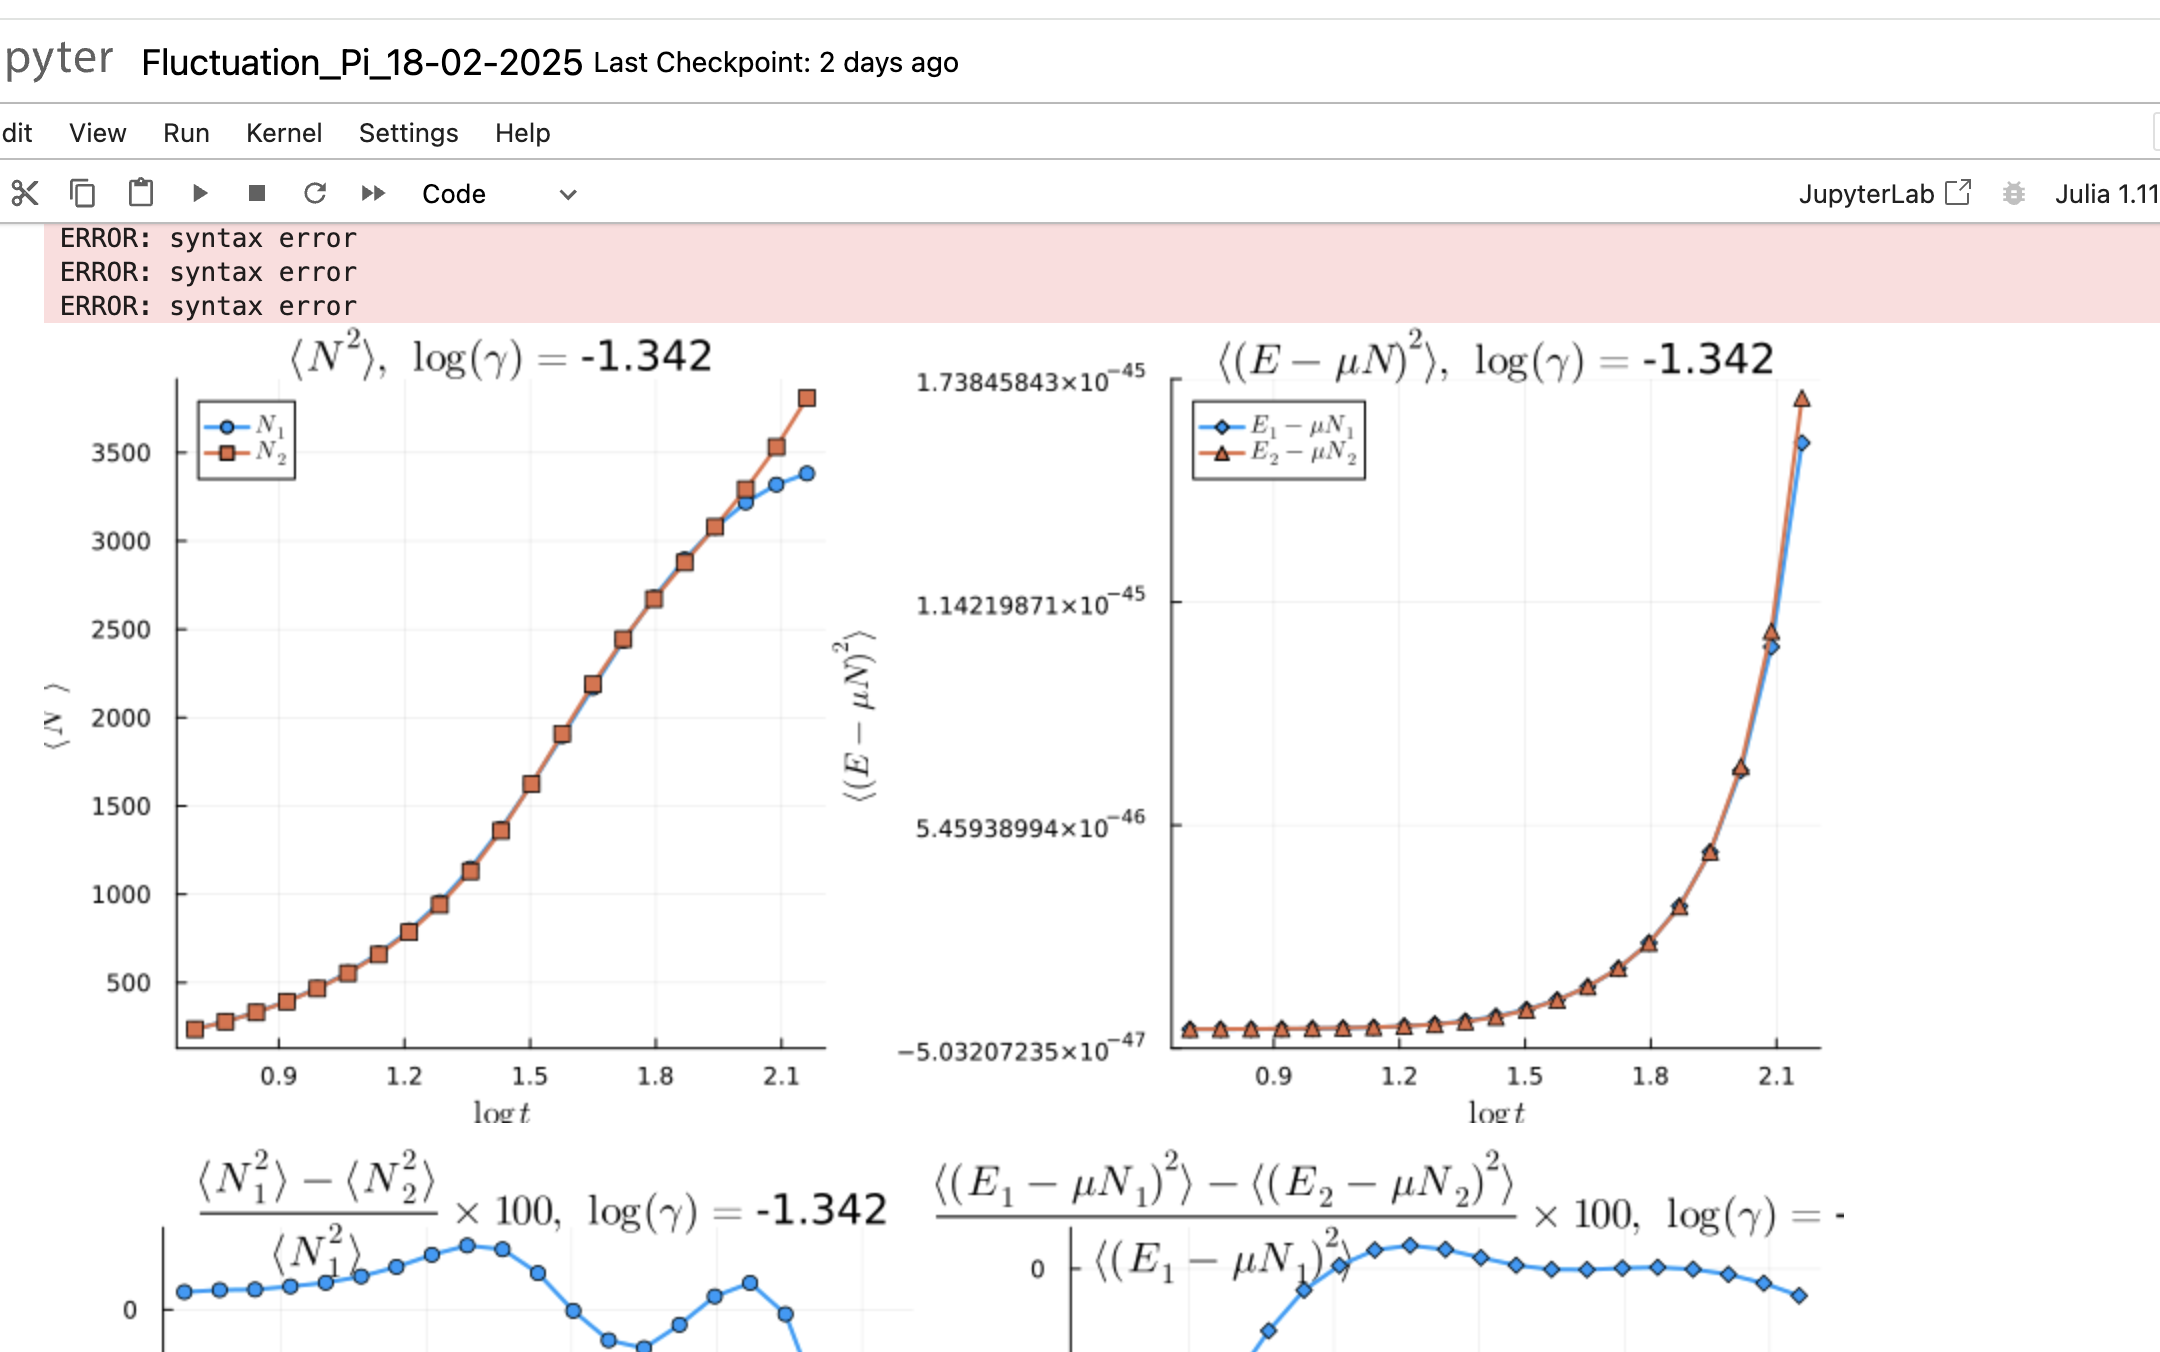
\includegraphics[width=1\textwidth]{Figures/test}

%\begin{aff}
%Donc une a l'ordre un en $\delta \theta (\operator{A}^{(0)})^{-1} %\operator{V}$ 

%\begin{eqnarray*}
%	\langle \delta \Pi ( \theta) \delta \Pi ( \theta') \rangle & = &  ( (\Pi^c_s - \Pi^c)\Pi^c/\Pi^c_s ) ( \theta ) \delta_{\theta, \theta'}/\delta \theta + \mathscr{F}(\theta , \theta' ) ,	
%\end{eqnarray*}

%avec 

%\begin{eqnarray*}
%	\mathscr{F}(\theta , \theta' ) & = & \left [ (\Pi^c_s - \Pi^c )( \theta)  +  (\Pi^c_s - \Pi^c ) ( \theta' )\right ] \frac{\Pi^c}{\Pi^c_s}(\theta)\frac{\Pi^c}{\Pi^c_s}(\theta') \frac{ \Delta( \theta'- \theta )}{ 2 \pi }\\
%	&&  - \left [ (\Pi^c_s - \Pi^c )( \theta)   (\Pi^c_s - \Pi^c ) ( \theta' )\right ] \frac{\Pi^c}{\Pi^c_s}(\theta)\frac{\Pi^c}{\Pi^c_s}(\theta')\int d\theta'' \left (   \frac{ \Pi^c/\Pi^c_s}{\Pi^c_s - \Pi^c} \right )(\theta'') \frac{\Delta(\theta''- \theta)}{2 \pi}\frac{\Delta(\theta''- \theta')}{2 \pi}  	
%\end{eqnarray*}
%\end{aff}



 








\chapter{Lien avec les équations de Bethe}
%Dans ce chapitre, nous nous intéressons aux fluctuations de la distribution de rapidité \( \delta \rho \) autour d'une distribution de référence \( \rho^c \), qui maximise la contribution à la fonction de partition des états, exprimée comme une fonctionnelle de la distribution \( \rho \) : 

La fonction de partition des états, s'exprime comme une fonctionnelle de la distribution \( \rho \) : 

\begin{eqnarray*}
	\Xi & = & \sum_\rho \exp \left( -\mathcal{A}(\rho) \right).
\end{eqnarray*}  

Dans la section {\em \bf Entropie de Yang-Yang} (\ref{??}), l'action \( \mathcal{A}(\rho) \) s'écrit sous la forme :  

\begin{eqnarray*}
	\mathcal{A}(\rho) & \doteq & - L\mathcal{S}_{YY}(\rho) + L\int f(\theta) \rho (\theta) \, d\theta,		
\end{eqnarray*}  

où \( \mathcal{S}_{YY} \) est la fonctionnelle d'entropie de Yang-Yang, définie dans (\ref{??}), et \( f \) est la fonction paramétrant les charges, introduite dans (\ref{??}).  

Dans cette même section {\em \bf Entropie de Yang-Yang} (\ref{??}), nous avons établi un lien entre \( f \) et distribution de référence \( \rho^c \), qui maximise la contribution à la fonction de partition des états .\\

On veux tester si nos experience est décrit pas un GGE. Pour cela nous nous intéressons aux fluctuations de la distribution de rapidité \( \delta \rho \) autour \( \rho^c \).

%Nous poursuivons à présent avec cette définition de l'action de classe $\mathcal{C}^2$ et admetant une distribution critique $\rho^c$ tel que sa différentielle en ce point critique soit nulle $d\mathcal{A}_{\rho^c} = 0 $ (\ref{??}) de sorte que d'aprés la formule de Taylor-Youg %afin de déterminer les fluctuations autour de \( \Pi^c \). Pour cela, nous réécrivons l'action sous la forme :  

Nous poursuivons à présent avec cette définition de l'action de classe $\mathcal{C}^2$ et admetant une distribution critique $\rho^c$ tel que sa différentielle en ce point critique soit nulle $d\mathcal{A}_{\rho^c} = 0 $ (\ref{??}) de sorte que d'aprés la formule de Taylor-Youg %afin de déterminer les fluctuations autour de \( \Pi^c \). Pour cela, nous réécrivons l'action sous la forme :  

\begin{eqnarray*}  
	\mathcal{A}(\rho^c + \delta \rho) & \underset{ \delta \rho \to 0 }{=} & \mathcal{A}(\rho^c)  + \frac{1}{2} \left. \frac{\delta^2 \mathcal{A}}{\delta \rho^2} \right|_{\rho^c} (\delta \rho) + \mathcal{O}((\delta \rho)^3),  
\end{eqnarray*}  

une expression quadratique pour l'action à l'ordre dominant en \( \delta \Pi \) avec $\left. \frac{\delta^2 \mathcal{A}}{\delta \rho^2} \right|_{\rho^c}$ la forme quadratique définie positive (Fig (\ref{fig.fluctu.A})).

\begin{figure}[H]
	\centering 
	\begin{tikzpicture}
		\begin{scope}[shift={(0,0)}]
			\begin{scope}[transform canvas={scale=0.6}]
				% Définition des couleurs avec les codes HTML
\definecolor{colorOne}{HTML}{443E46}
\definecolor{colorTwo}{HTML}{F6DEB8}
\definecolor{colorThree}{HTML}{908CA4}
\definecolor{colorFour}{HTML}{57659E}
\definecolor{colorFive}{HTML}{C57284}
\definecolor{colorSix}{HTML}{FF5B69}

% Raccourcis pour les couleurs
\def\colorOne{colorOne}
\def\colorTwo{colorTwo}
\def\colorThree{colorThree}
\def\colorFour{colorFour}
\def\colorFive{colorFive}
\def\colorSix{colorSix}

\def\colorslide{blue!50!black}



\begin{scope}
	% Tracer une courbe lisse entre des points
	\draw[shift={(0,0)} ,\colorOne]
		(-1 , 0 ) edge [thick,line width=0.8ex , ->,>=triangle 45  , \colorOne] node [pos = 1 , below ]{\huge$\rho$}( 5  , 0 )
	;
	\draw[shift={(0,0)}, color=\colorOne]
		(0, -1.0 ) edge [thick,line width=0.8ex , ->,>=triangle 45  ]node [pos=0.9,left=0.2cm ]{\huge$\mathcal{A}(\rho)$}( 0  , 5 )
	;
	\draw[]
		(2.5, 0.12 ) edge [thick,line width=0.8ex ,\colorThree ]node [pos=1,below  ]{\huge$\rho^c$} (2.5, -0.12 )	
	;
	
	\draw[]
		(2.5, -0.12 ) edge [thick,line width=0.4ex , dashed, \colorThree ] (2.5, 5.5 )
		(1.5, 1 ) edge [thick,line width=0.4ex , <->,>=triangle 45  , \colorThree ] (3.5, 1 )
		(-0.3,1) edge [thick,line width=0.4ex  , \colorThree ] node [pos=0,left ]{\huge$\mathcal{A}(\rho^c)$} (0.3, 1 )	
	;
    \draw[thick, line width=0.8ex , \colorFour] plot[smooth, tension=0.7] coordinates {
        (1, 5) (1.6 , 3 ) (2.5, 1) (3.5 , 3 )  (4, 5)
    };		
	
\end{scope}

	
			
			\end{scope}
			
			\draw[color = red , scale = 0.5 , draw = none  ] (-2 , -1) rectangle (5, 6) ; 	
		\end{scope}
		
		\begin{scope}[shift={(19,-1)}]
			\begin{scope}[transform canvas={scale=0.6}]
				% Définition des couleurs avec les codes HTML
\definecolor{colorOne}{HTML}{443E46}
\definecolor{colorTwo}{HTML}{F6DEB8}
\definecolor{colorThree}{HTML}{908CA4}
\definecolor{colorFour}{HTML}{57659E}
\definecolor{colorFive}{HTML}{C57284}
\definecolor{colorSix}{HTML}{FF5B69}

% Raccourcis pour les couleurs
\def\colorOne{colorOne}
\def\colorTwo{colorTwo}
\def\colorThree{colorThree}
\def\colorFour{colorFour}
\def\colorFive{colorFive}
\def\colorSix{colorSix}

\def\colorslide{blue!50!black}

\def\Occupation{
	\def\traitx{0.3}
	\def\traity{0.5}
	\draw[shift={(0,0)}]
		(-13.5 , 0 ) edge [thick,line width=0.8ex ]( -3.2  , 0 )
		( -3.2 - \traitx  , 0 - \traity ) edge [thick,line width=0.8ex ]( -3.2 + \traitx  , 0 + \traity  )
		( -2.8 - \traitx  , 0 - \traity ) edge [thick,line width=0.8ex ]( -2.8 + \traitx  , 0 + \traity  )
		(-2.8 , 0 ) edge [thick,line width=0.8ex ](2.8  , 0 )
		( 2.8 - \traitx  , 0 - \traity ) edge [thick,line width=0.8ex ]( 2.8 + \traitx  , 0 + \traity  )
		( 3.2 - \traitx  , 0 - \traity ) edge [thick,line width=0.8ex ]( 3.2 + \traitx  , 0 + \traity  )
		(3.2, 0 ) edge [thick,line width=0.8ex,->,>=triangle 45 , color = black ]node [pos=1.01,below  ]{\huge$\theta$}	( 13  , 0 )
	;
	\draw[shift={(0,0)}, color=\colorOne]
		(-10.5 , -1.5 ) edge [thick,line width=0.8ex , ->,>=triangle 45  ]( -10.5  , 4.5 )
	;
		
	\foreach \r in {1 , ... , 3 } {
%		\draw[
%		decoration={
%		markings,
%    	mark connection node=my node,
%    	mark=at position 0 with{\node [blue,transform shape] (my node) {\large \r};}},
%		color=gray, thick, 
%		line width=0.5ex] decorate { 
%            (-11.0, \r) -- (-10.1, \r )}
%        ;
        \draw[
			color=\colorOne,
			] 
            (-11.0, \r) edge[color=\colorThree , thick,line width=0.5ex] node [pos=-0.5 ]{\large\color{\colorFour} $\frac{\r}{\delta \theta}$ } (-10.3, \r )
        	;
	
	}
	

	
	% Graduation abcsisse 
	% Définitions des listes
% Definitions of the lists
\def\listetuple{-9/\theta_{1}, -8/\theta_{2} , -5/\theta_{3} , -2/\theta_{a-1} , 0/\theta_{a} , 1/\theta_{a+1} , 2/\theta_{a+2} ,  5/\theta_{N-4} , 7/\theta_{N-3},8/\theta_{N-1},9/\theta_{N} }
\def\listetrais{-12 , -11, -10, -9 , -8 , -7 ,  -6 , -5, -4.5,-4, -2 , -1, 0 , 0.5, 1, 2, 4 , 5 ,  6 , 7 , 8 ,8.5, 9 ,  10 , 11, 12 }

% Loop over listetrais
\foreach \r in \listetrais {
    % Initialize found variable to zero
    % Initialize found variable to zero
    %\pgfmathsetmacro\found{0}
    \global\def\found{0}
    \xdef\nomtheta{}
    
    % Check if \r is in listetuple
    \foreach \x/\y in \listetuple { 
        \ifdim \r pt=\x pt % If \r matches any \x in listetuple
            \global\def\found{1} ;
            \xdef\nomtheta{\y} % Set \nomtheta to the corresponding \y
            %\pgfmathsetmacro\found{1} % Set found to 1            
            %\global\pgfmathsetmacro\found{1}
        \fi
    }
    
    %\node [circle, draw, red] (A) at (\r, 2) {\found , $\nomtheta$};
    
    % Draw the line and display \nomtheta if found
    \ifnum\found=1
        \draw[color=\colorOne, thick, line width=0.5ex] 
            (\r, -0.3) -- (\r, 0.3) node[red , pos=-0.5] {\large $\nomtheta$};
         \filldraw[line width=0.5ex, color=\colorSix, outer color=\colorSix, inner color=\colorSix] 
            (\r, 0) circle (4pt);
    \else 
        % Draw without \nomtheta and add a blue circle if not found
        \draw[color=\colorOne, thick, line width=0.5ex] 
            (\r, -0.3) -- (\r, 0.3);
        \filldraw[line width=0.5ex, color=\colorSix, outer color=\colorTwo, inner color=\colorTwo] 
            (\r, 0) circle (4pt); 
    \fi
}

\def\listetrais{-9.5/\theta_{i-1}/2/3, -6.5/\theta_{i}/1/4  ,   -1.5/\theta_{j}/2/4 , 1.5/\theta_{j+1}/-1/3 , 3.5/\theta_{\ell-1}/1/3 , 6.5/\theta_{\ell}/3/4 , 9.5/\theta(\theta_{\ell+1})/-1/3 };



\foreach \r/\nomx/\y/\ys in \listetrais {
	\draw[
		decoration={
		markings,
    	mark connection node=my node,
    	mark=at position .5 with{\node [blue,transform shape] (my node) {\large \color{\colorFour} $\nomx$};}},
		color=\colorThree , thick, 
		line width=0.5ex] decorate { 
            (\r, 0.12) -- (\r, -1.2)}
        ;
     
     \ifdim \y pt > -1 pt 
     	\draw[
			decoration={
			markings,
    		mark connection node=my node,
    		mark=at position .5 with{\node [blue,transform shape] (my node) {\large \color{\colorFour} $\Pi(\nomx) $};}},
			color=\colorThree, thick, 
			line width=0.5ex] decorate { 
            (\r, \y) -- (\r +3, \y)}
        ;
        \draw[
			decoration={
			markings,
    		mark connection node=my node,
    		mark=at position .5 with{\node [blue,transform shape] (my node) {\large \color{\colorFive} $\Pi_s(\nomx) $};}},
			color=\colorFive, thick, 
			line width=0.5ex] decorate { 
            (\r, \ys) -- (\r +3, \ys)}
        ;
     \fi 
     \ifdim \r pt= -1.5 pt
     	\draw[
     		decoration={
			markings,
    		mark connection node=my node,
    		mark=at position .5 with{\node [blue,transform shape] (my node) {\large \color{\colorFour}  $\delta \theta $};},
    		%mark=at position 0.1  with {\arrow[blue, line width=0.5ex]{<}},
    		%mark=at position 1  with {\arrow[blue, line width=0.5ex]{>}}
    		},
        	color=\colorThree,
        	thick,
        	line width=0.5ex,
        	%arrows={Computer Modern Rightarrow[line cap=round]-Computer Modern Rightarrow[line cap=round]}
   			](\r, -1.2) edge[arrows={Computer Modern Rightarrow[line cap=round]-}] (\r + 0.4, -1.2)decorate {
    		(\r, -1.2) -- (\r + 3, -1.2)}(\r + 2, -1.2) edge[arrows={-Computer Modern Rightarrow[line cap=round]}] (\r + 3, -1.2)
    		;
    \fi
			
	
}


			
}


\begin{scope}
	%\draw[help lines , width=1.5ex] (-8,-3) grid (8,3);\draw[help lines ,width=0.5ex , opacity = 0.5] (-3,-3) grid[step=0.1] (3,3));
	
	%\draw[help lines] 
	%	(-3,-3) edge[width=1.5ex] grid (3,3)	
	%	(-3,-3) edge[width=0.5ex , opacity = 0.5] grid (3,3)	
	%;
	\begin{scope}[shift={(0,1)},rotate=0,opacity=1,color=black]
		\Occupation	
		
		%\node[anchor=east, font=\bfseries] at (-11, 0) {\color{red}\large (T = 0 )} ;	
	\end{scope}
	
	
	
	
	\begin{scope}[shift={(-10.5,7)},rotate=0,opacity=1,color=black]
	
	\begin{scope}[shift={(-0,0)},rotate=0,opacity=1,color=black]
	
		\draw[shift={(0,0)} ,line width=1ex,rounded corners = 1ex,color=\colorOne , opacity =1 ,fill=\colorOne!00 , pattern={north east lines} , pattern color=\colorOne!00 ]
			(0 , -1 ) rectangle (5,1)
		;
		

		\begin{scope}[shift={(0.5,0.5)}]
			\draw[color=\colorOne, thick, line width=0.5ex] 
            (0, -0.3) -- (0, 0.3) ;
            \filldraw[line width=0.5ex, color=\colorSix, outer color=\colorSix, inner color=\colorSix] 
            (0, 0) circle (4pt);
            
            \node[anchor=west, font=\bfseries] at (0.2, 0) {\color{\colorSix}\large : quasi-particule};
		\end{scope}
		
		\begin{scope}[shift={(0.5,-0.5)}]
			\draw[color=\colorOne, thick, line width=0.5ex] 
            (0, -0.3) -- (0, 0.3) ;
            \filldraw[line width=0.5ex, color=\colorSix, outer color=\colorTwo, inner color=\colorTwo] 
            (0, 0) circle (4pt);
            
            \node[anchor=west, font=\bfseries] at (0.2, 0) {\color{\colorSix}\large : hole};
		\end{scope}

	\end{scope}
	
	\begin{scope}[shift={(6,0)},rotate=0,opacity=1,color=black]	
		
		\draw[shift={(0,0)} ,line width=1ex,rounded corners = 1ex,color=\colorOne , opacity =1 ,fill=\colorOne!00 , pattern={north east lines} , pattern color=\colorOne!00 ]
			(0 , -1 ) rectangle (7.5,1)
		;
		
		\node[anchor=west] at (0.5, 0.5) {\color{\colorFour}\large $\Pi$ };\node[anchor=west, font=\bfseries] at (1, 0.5) {\color{\colorFour}\large : quasi-particule distribution};
		
		\node[anchor=west] at (0.5, -0.5) {\color{\colorFour}\large $\Pi_h$ };\node[anchor=west, font=\bfseries] at (1, -0.5) {\color{\colorFour}\large  : hole distribution};
		
	\end{scope}
	
	\begin{scope}[shift={(14.5,0)},rotate=0,opacity=1,color=black]	
		
		\draw[shift={(0,0)} ,line width=1ex,rounded corners = 1ex,color=\colorOne , opacity =1 ,fill=\colorOne!00 , pattern={north east lines} , pattern color=\colorOne!00 ]
			(0 , -0.5 ) rectangle (7.0,0.5)
		;
		
		\node[anchor=west] at (0.2, 0) {\color{\colorFour}\large ${\color{\colorFive}\Pi_s} = \Pi + \Pi_h $ } node[anchor=west , font=\bfseries] at (3.1 , 0 )  {\color{\colorFour}\large {\color{\colorFive} : density of states}};
		
	\end{scope}
	
	
	\end{scope}


		
	
\end{scope}

	
			
			\end{scope}
			\begin{scope}[scale=1]
				\draw[color = red , scale = 1 , draw = none  ] (-1 , -1) rectangle (5, 5) ; 
			\end{scope}	
		\end{scope}

		
				
			
	\end{tikzpicture}	
	\captionsetup{skip=10pt} % Ajoute de l’espace après la légende
	\label{fig.fluctu.A}
\end{figure}


On discrétise l'axe des rapidités en  petite cellule de rapidité $[\theta, \theta+\delta\theta]$, qui contient $L\rho(\theta) \delta \theta$ rapidités. 
	



Avec ces petites tranches, la forme quadratique s’écrit :

\begin{eqnarray*}
    \left. \frac{\delta^2 \mathcal{A}}{{\delta \rho}^2} \right|_{\rho^c}(\delta \rho ) &=&  \sum_{a,b \mid \text{tranche}}  
    \delta \rho(\theta_a)  \frac{\partial^2 \mathcal{A}}{\partial \delta \rho(\theta_a) \partial \delta \rho(\theta_b) } (\rho^c)  \delta \rho(\theta_b).
\end{eqnarray*}
Les fluctuations s’écrivent donc :

\begin{eqnarray*}
    \langle \delta \rho ( \theta) \delta \rho ( \theta') \rangle &=&  
    \frac{ \int d\delta \rho \, \delta \rho(\theta) \delta \rho ( \theta') 
    \exp \left( - \frac{1}{2} \sum_{a,b \mid \text{tranche}}  
    \delta \rho(\theta_a) \frac{\partial^2 \mathcal{A}}{\partial \delta \rho(\theta_a) \partial \delta \rho(\theta_b) } (\rho^c)  \delta \rho(\theta_b) \right) }
    { \int d\delta \Pi  
    \exp \left( - \frac{1}{2} \sum_{a,b \mid \text{tranche}}  
    \delta \rho(\theta_a) \frac{\partial^2 \mathcal{A}}{\partial \delta \rho(\theta_a) \partial \delta \rho(\theta_b) } (\rho^c)  \delta \rho(\theta_b) \right) } \\
    &=& \left( \mathbf{A}^{-1} \right)_{\theta , \theta'}
\end{eqnarray*}


\begin{aff}

\begin{eqnarray*}
	\langle \delta \rho ( \theta) \delta \rho ( \theta') \rangle &=& 	\left( \mathbf{A}^{-1} \right)_{\theta , \theta'}
\end{eqnarray*}

	
avec la  {\em matrice hessienne} $\mathbf{A}_{\theta , \theta'} \equiv \frac{\partial^2 \mathcal{A}}{\partial \delta \rho(\theta) \partial \delta \rho(\theta') }(\rho^c)$, au point critique/ qui maximise la probabilité  $\rho^c=\rho^c_s \nu^c $, s'écrit

\begin{eqnarray*}
	\operator{A} & = & \operator{A}^{(0)} + \delta \theta \operator{V}
\end{eqnarray*}

avec 

\begin{eqnarray*}
	A^{(0)}_{\theta , \theta'}  & = &  L\delta \theta \left ( \frac{ 1}{\rho^c_s ( 1  - \nu^c ) \nu^c } \right )(\theta)    \delta({\theta - \theta '})	,\\
	V_{\theta , \theta'}  &= & L \delta \theta \left \{ - \left [ \left ( \frac{1}{\rho^c_s( 1 - \nu^c) } \right ) ( \theta)  +  \left ( \frac{1}{\rho^c_s( 1 - \nu^c) } \right ) ( \theta' )\right ] \frac{ \Delta( \theta'- \theta )}{ 2 \pi } + \int d\theta''  \left ( \frac{\nu^c}{\rho^c_s( 1 - \nu^c) } \right )(\theta'') \frac{\Delta(\theta''- \theta)}{2 \pi}\frac{\Delta(\theta''- \theta')}{2 \pi}   \right \} 	
\end{eqnarray*}

\end{aff}

\subsection{Testes}

\begin{eqnarray*}
	\Delta_{\operator{\mathcal{N}}}^2  & = &  \frac{1}{\beta} \left . \frac{\partial \langle \operator{\mathcal{N}} \rangle}{\partial \mu} \right )_T \\
	\Delta_{\operator{\mathcal{E}}-\mu \operator{\mathcal{N}}}^2  & = &  - \left . \frac{\partial \langle \operator{\mathcal{E}}-\mu \operator{\mathcal{N}} \rangle}{\partial \beta} \right )_\mu 
\end{eqnarray*}

et 

\begin{eqnarray*}
	\Delta_{\operator{\mathcal{N}}}^2  &= & L^2 \int d\theta_a \int d \theta_b \, \langle \delta \rho(\theta_a) \delta \rho(\theta_b) \rangle \\
	\Delta_{\operator{\mathcal{E}}-\mu \operator{\mathcal{N}}}^2  & = & L^2 \int d\theta_a \int d \theta_b \, \left ( - \mu + \frac{1}2 m \theta_a^2  \right  )\left ( - \mu + \frac{1}2 m \theta_b^2  \right  )  \langle \delta \rho(\theta_a) \delta \rho(\theta_b) \rangle
\end{eqnarray*}

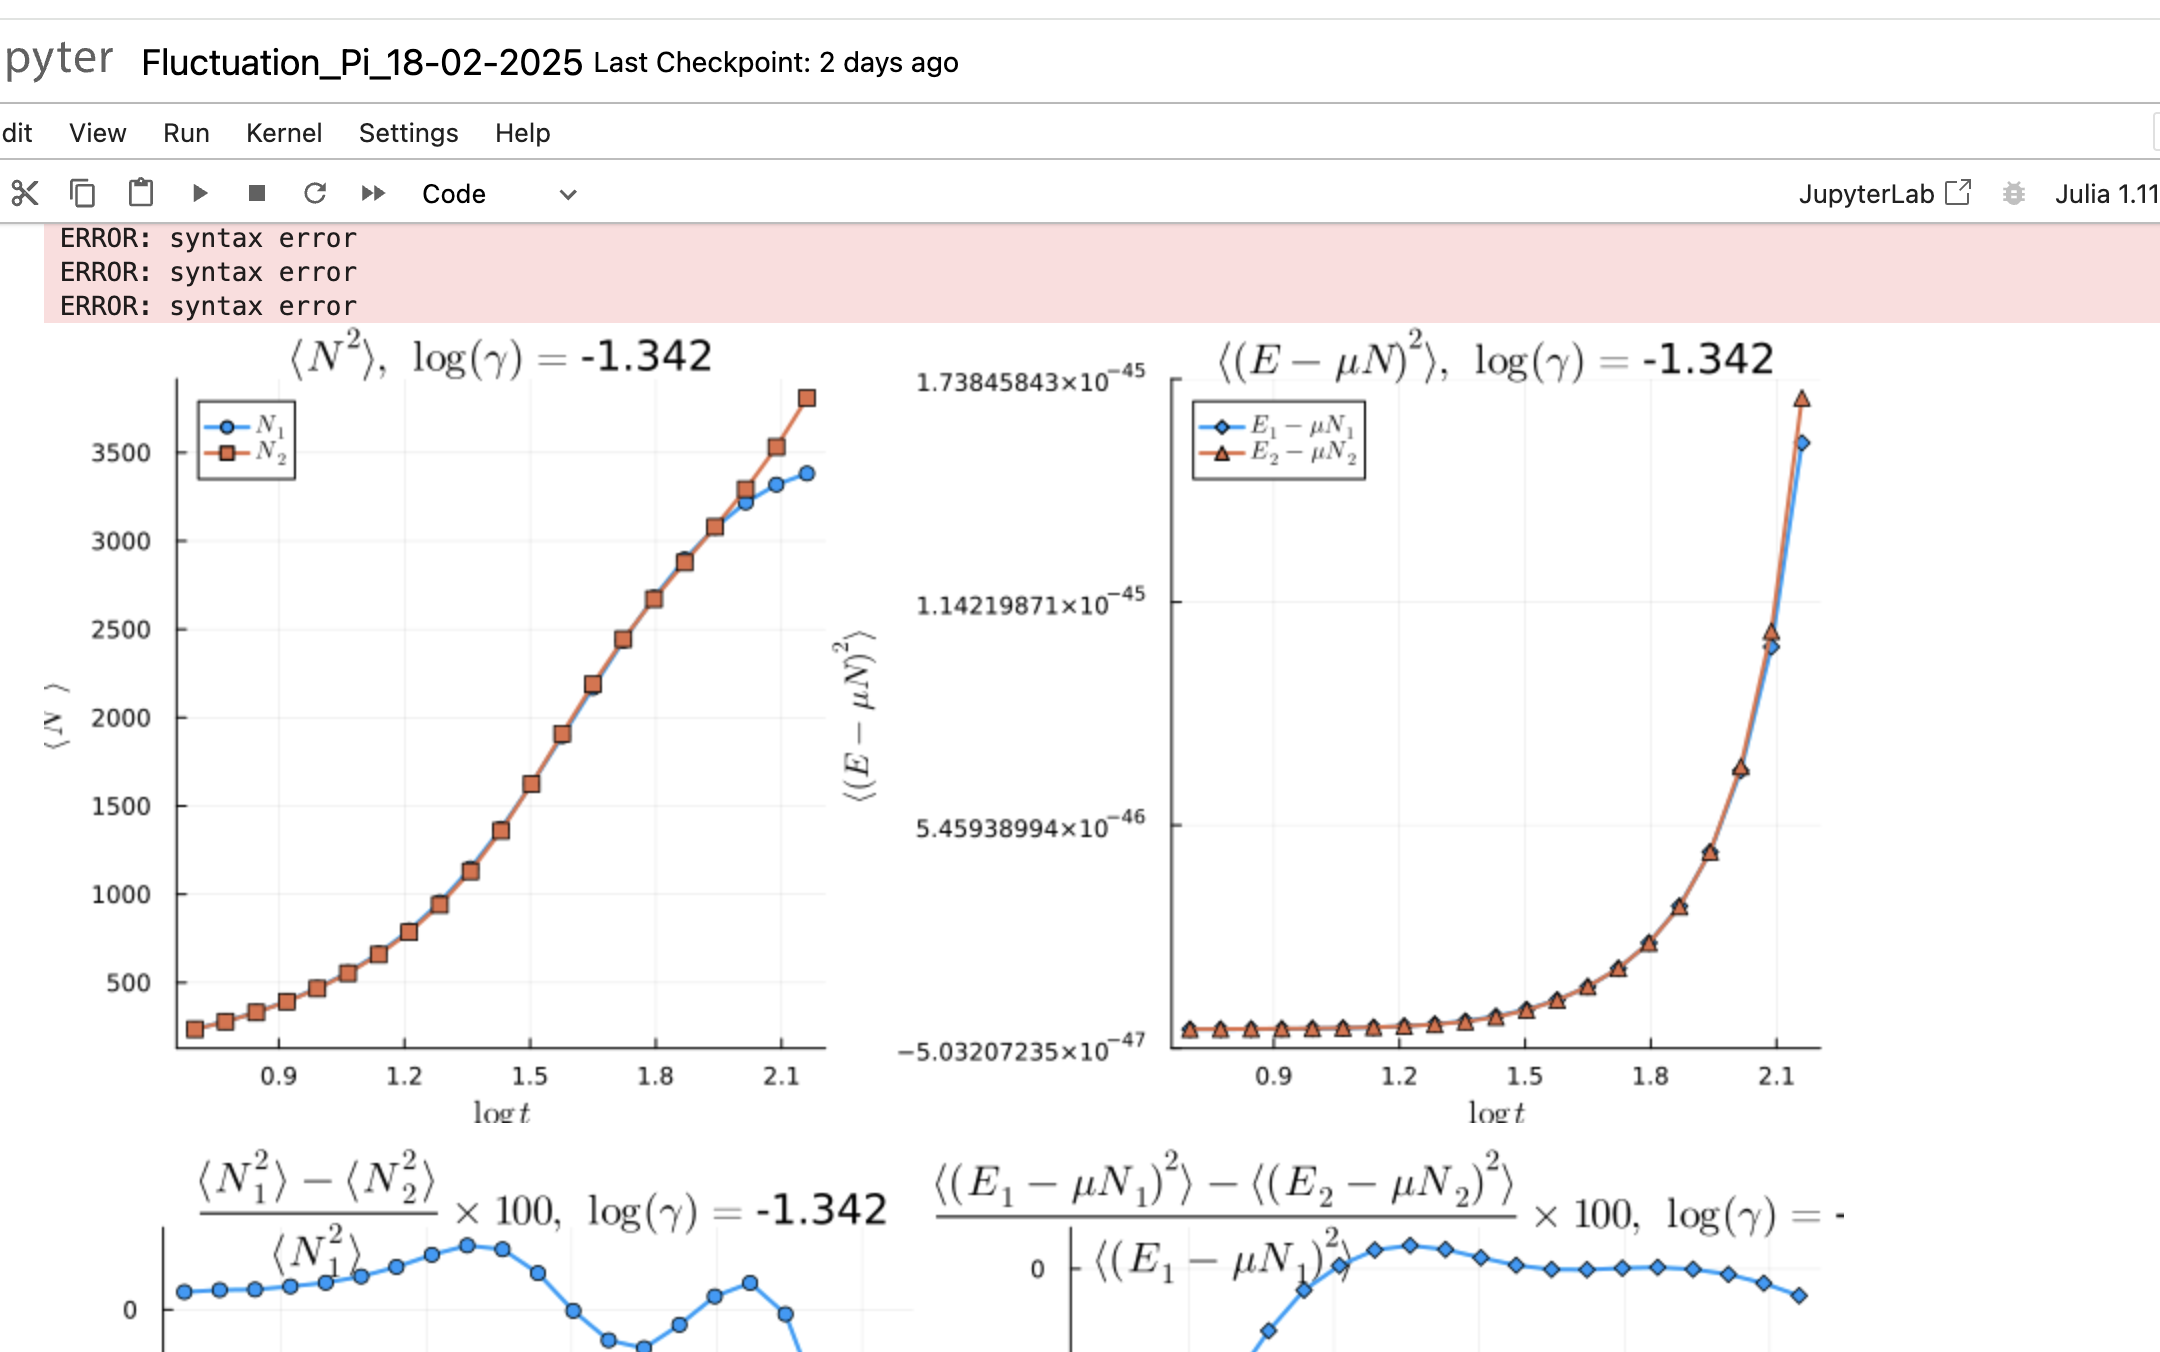
\includegraphics[width=1\textwidth]{Figures/test}

%\begin{aff}
%Donc une a l'ordre un en $\delta \theta (\operator{A}^{(0)})^{-1} %\operator{V}$ 

%\begin{eqnarray*}
%	\langle \delta \Pi ( \theta) \delta \Pi ( \theta') \rangle & = &  ( (\Pi^c_s - \Pi^c)\Pi^c/\Pi^c_s ) ( \theta ) \delta_{\theta, \theta'}/\delta \theta + \mathscr{F}(\theta , \theta' ) ,	
%\end{eqnarray*}

%avec 

%\begin{eqnarray*}
%	\mathscr{F}(\theta , \theta' ) & = & \left [ (\Pi^c_s - \Pi^c )( \theta)  +  (\Pi^c_s - \Pi^c ) ( \theta' )\right ] \frac{\Pi^c}{\Pi^c_s}(\theta)\frac{\Pi^c}{\Pi^c_s}(\theta') \frac{ \Delta( \theta'- \theta )}{ 2 \pi }\\
%	&&  - \left [ (\Pi^c_s - \Pi^c )( \theta)   (\Pi^c_s - \Pi^c ) ( \theta' )\right ] \frac{\Pi^c}{\Pi^c_s}(\theta)\frac{\Pi^c}{\Pi^c_s}(\theta')\int d\theta'' \left (   \frac{ \Pi^c/\Pi^c_s}{\Pi^c_s - \Pi^c} \right )(\theta'') \frac{\Delta(\theta''- \theta)}{2 \pi}\frac{\Delta(\theta''- \theta')}{2 \pi}  	
%\end{eqnarray*}
%\end{aff}



 










\newpage
\printindex
\printindex[pers]
			            
\end{document}